\documentclass{book}

\usepackage[utf8]{inputenc}
\usepackage[english]{babel}

\usepackage{graphicx}
\usepackage{epsfig}
\usepackage{algorithm}
\usepackage{amsmath}
\usepackage{amsfonts}
\usepackage{psfrag}
\usepackage[dvips]{color}
\usepackage{pstricks,pst-node,pst-plot,pst-tree}
\usepackage{hyperref}

\title{CSCI 104: Data Structures and Object-Oriented Design}
\author{David Kempe}

\newtheorem{theorem}{Theorem}[section]
\newtheorem{corollary}{Corollary}[theorem]
\newtheorem{lemma}[theorem]{Lemma}
\newtheorem{example}{Example}[section]


\begin{document}


\begin{titlepage}
\maketitle
\end{titlepage}


\chapter*{Preface}
\label{chapter:preface}
These lecture notes grew out of class notes provided for the students
in CSCI 104 (``Data Structures and Object-Oriented Design'') 
at the University of Southern California in Fall of 2013.
The class is typically taken in the second semester of freshman year
or the first semester of sophomore year. Students are expected to be
familiar with structural programming in the C++ programming language,
the basics of dynamic memory management, and recursion.
Brief refreshers on these two specific topics are included at the
beginning of the notes, and typically covered for about one lecture
each, but a student not already familiar with these concepts is likely
to struggle in the class.

These notes represent the specific way in which we like to present the
material, by motivating object-oriented design primarily from the
point of view of implementing data structures. There is perhaps
somewhat more focus on analysis and allusions to advanced topics than
in a typical programming-heavy data structures course for undergraduates.
The notes are, at least at present, not intended to replace an actual
detailed textbook on data structures. 
We currently use the book ``Data Abstraction and Problem Solving'' by
Carrano and Henry.

The notes are based on lecture notes taken by the CSCI 104 course
producers in Fall 2013:
Chandler Baker, Douglass Chen, Nakul Joshi, April Luo, Peter Zhang,
Jennie Zhou.
Douglass was the main notetaker, in charge of about half of the notes
himself, and coordinating the others' notes as well.
The notes were subsequently expanded significantly by David Kempe,
and then expanded further and reorganized again for subsequent semesters,
when they took essentially their current form.


\tableofcontents


\chapter{Overview}
\label{chapter:overview}
If you've gotten this far, you are expected to be familiar with the basics of programming C++.
Consider features such as:

\begin{itemize}
	\item Primitive data types: \texttt{int}, \texttt{string}, \texttt{float}, \texttt{double}, etc.
	\item Composite data types: arrays, \texttt{struct}.
	\item Control statements: \texttt{for}, \texttt{while}, \texttt{do while}, \texttt{if}, \texttt{else}, and \texttt{switch}.
	\item Functions: declaration, iteration vs. recursion.
\end{itemize}

In principle, these features are enough to solve any programming problem.
In fact, in principle, it is enough to have nothing except for \texttt{if}, \texttt{while}, integers, and arithmetic.
Everything beyond those basics is "just" there to help us write code that is better, faster, more easily maintained, or more easily understood.

Of course, these are all fairly critical aspects of programming in the real world.
Consequently, there is great value in continuing past basic proficiency, and in order to do so, we will focus on two categories of things we can learn that will help us on our way:

\begin{enumerate}
\item Ideas, techniques, and patterns that enable us to solve problems that we didn't know how to solve (even though we had the tools to).
\item Language features and programming concepts that help us write code that is easy to read, debug, and extend.
\end{enumerate}

At this stage, you might think about programming in terms of the data your program interacts with: data is input, the program executes commands, and some corresponding output data is produced.
In this context, the sequence of instructions, i.e. the \emph{algorithm}, is the emphasis of our thought process.

The goal of this class, and by extension, this textbook, is teach you how to emphasize how data is transformed throughout the execution of a program.
We will cultivate this skill by examining new ideas, techniques, and patterns in the form of data structures, and you will learn to express them through the lens of object-oriented programming by learning new C++ language features and programming concepts.
Along the way, you will see how thinking about the organization of your data can provide insight into the efficiency of your programs.
Ultimately, this will enable you to write code that is more maintainable, easier to understand, and potentially faster.

\section{An Example}

\begin{displayquote}
Two TAs each get a list of the names and emails of the students in the class.
One gets the list sorted alphabetically, while the other gets it randomly shuffled.
Both TAs are asked to look up the email of one particular student by name.
Who would you expect to be faster at the task?
Except in rare cases, the TA with the sorted list will be much faster, and indeed, this is what happens when we run this experiment in the classroom. 
\end{displayquote}

The way we organize our data can have a profound impact on how fast (or slowly) we can solve a computational task. 
\emph{How we organize data to support the operations we need is the centerpiece of what you will learn in this class.}

What do we mean by "support the operations we need"?
Let's go back to the example of looking up emails of students by name.
Here, the key operation is clearly the "lookup" operation, at least from the standpoint of the student doing the looking up.
But when we look at the bigger picture, those data items (pairs of a student name and an email) had to be added into that form somehow.
And sometimes, we may want to delete them.
So really, the three operations we are interested in are:

\begin{itemize}
\item Insert a pair of a name and email into the list.
\item Remove a name from the list.
\item Look up the email for a given name.
\end{itemize}

Purely from the perspective of speeding up the lookup operation, the sorted list was much better than the unsorted one.
But in terms of inserting items, it is clearly better to keep the list unsorted, as we can just append items at the end of the list, and not have to worry about putting the item in the right place.
For removal---well, you will learn about that a little more later.

It is easy to imagine scenarios where keeping the list sorted is not worth it.
If we need to add data items all the time but very rarely look them up (say, some kind of backup mechanism for disasters), then sorting the list is not worth it.
Or perhaps the list is so short that even scanning through all the items is fast enough.

The answer to "what is the best way to organize my data?" is almost always "it depends."
You will need to consider how you will be interacting with your data and design an appropriate data structure \emph{in the context of its purpose}. 
Will you be searching through it often?
Will data be added in frequent, short chunks, or in occasional huge blocks?
Will you ever have to consolidate multiple versions of your data structure?
What kinds of queries will you need to ask of your data?

\medskip

There is another interesting observation we can take away from the previous
example. We said that we wanted our data structure to support
the operations \texttt{add}, \texttt{remove}, and \texttt{lookup}.
Let us be a little more general than just thinking about a list of students.
\begin{itemize}
\item The \texttt{add (key, value)} operation gets a \emph{key} and a
  \emph{value}. (In our case, they were both strings, but in general,
  they don't have to be.)
  It creates an association between the key and value.
\item The \texttt{remove (key)} operation gets a key, and removes the
  pair that has the given key.
\item The \texttt{lookup (key)} operation gets a key, and returns the
  corresponding value, assuming the key is in the structure.
\end{itemize}
This type of data structure is typically called a \emph{map},
or a \emph{dictionary}.

So is a sorted list a map? Not exactly.
After all, an unsorted list would also be a map.
There seems to be a difference.
The main difference is that the word ``map'' describes the
\emph{functionality} that we want:
\emph{what} the data structure is supposed to do.
On the other hand, a sorted list (or an unsorted list) is a
\emph{specific way} of getting this functionality:
it says \emph{how} we do it. 

This distinction is very important. When you start to program,
usually, you just go straight ahead and plan out all of your code.
As you take on bigger projects, work in larger teams, and generally
learn to think more like a computer scientist, you get used to the 
notion of \emph{abstraction}: separating the ``what'' from the ``how.''
You can work on a project with a friend, and tell your friend
which functions you need from him/her, without having to think through
how they will be implemented. That is your friend's job.
So long as your friend's implementation works (fast enough) and meets
the specification that you prescribed (say, in terms of which order
the parameters are in), you can just use it as is.

So the way we would think about a map or dictionary is mostly in terms
of the functions it provides:
\texttt{add}, \texttt{remove}, and \texttt{lookup}.
Of course, it must store data internally in order to be
able to provide these functions correctly, but how it does that is
secondary --- that is part of the implementation.
This combination of data and code, with a well-specified interface of
functions to call, is called an \emph{abstract data type}.

Once you start realizing the important role that data organization
(such as using abstract data types) plays in good code design,
you may change the way you think about code interacting with data.
When starting to program, you probably thought about code that gets
passed some data (arrays, structs, etc.) and processes them.
Instead, you may now think of the data structure itself as having functions
that help with processing the data in it. 
In this way of thinking, an array in which you can only add things at
the end is different from one in which you are allowed to overwrite
everywhere, even though the actual way of storing data is the same.

This leads us naturally to \emph{object-oriented design} of programs. 
An \emph{object} consists of data and code; it is basically a
\texttt{struct} with functions inside in addition to the data fields. 
This opens up a lot of ideas for developing more legible,
maintainable, and ``intuitive'' code.
Once you think about objects, they often become almost like little
people in your mind.
Different objects serve different purposes,
and they interact with each other in particular ways.

One of the main things that thinking in terms of object-oriented
design (and abstract data types) does for you is to help achieve 
\emph{encapsulation}: shielding as much of the inside of an object as
possible from the outside, so that it can be changed without
negatively affecting the code around it.
The textbook refers to this as ``walls'' around data.
Encapsulation helps you achieve modularity, i.e., it ensures that
different pieces of code can be analyzed and tested in isolation more 
easily.

\medskip

To summarize, the learning goals of this class are:
\begin{enumerate}
\item Learn the basic and advanced techniques for actually
  implementing data structures to provide efficient functionality.
  Some of these techniques will require strong fundamentals,
  and their analysis will enter into more mathematical territory,
  which is why we will be drawing on material you will be learning
  simultaneously in CSCI 170.
\item Learn how to think about code more abstractly, separating the
  ``what'' from the ``how'' in your code design and utilizing abstract
  data types to specify functionality.
\item Learn about good programming practice with object-oriented
  design, in particular as it relates to implementing datatypes.
\end{enumerate}

%\section{Exercises}

\subsection{\ReviewQuestions}

\begin{exercise}
  Given that you can program all algorithms using just numbers,
  \code{while}, \code{if}, and arithmetic, what's the point of having
  other constructs for a programming language?
\end{exercise}

\begin{exercise}
  What do you call a combination of data and functions, abstractly
  specified?
\end{exercise}

\begin{exercise}
  What is a natural programming mechanism to \emph{implement} a
  combination of data and functions?
\end{exercise}

\begin{exercise}
  What are the three key operations supported by the \code{map} data
  type?
\end{exercise}

\begin{exercise}
  What is the difference between a sorted list and a map?
\end{exercise}

\begin{exercise}
  What kind of factors can contribute to determining which of several
  data structures to use to implement a particular abstract data type?
  Can you think of some that are not listed in the preceding chapter?
  (Hint: there are many.)
\end{exercise}

\begin{exercise}
  What does ``encapsulation'' mean for coding? Why is it a good thing?
\end{exercise}

\begin{exercise}
  At a high level, what are the important things you are supposed to
  learn in this class?
\end{exercise}



\chapter{Memory and Its Allocation}
\label{chap:dynamic-memory}
[Note: this chapter covers material of about 1 lecture.]

%At the physical level, computer memory consists of a large number of
flip flops.
Each flip flop consists of a few transistors,
and is capable of storing one bit.
Individual flip flops are addressable by a unique identifier,
so we can read and overwrite them. 
Thus, conceptually, we can think of all of our computer's memory as
just one giant array of bits that we can read and write.

Since as humans, we are not that good at doing all of our thinking and
arithmetic in bits, we group them into larger groups,
which together can be used to represent numbers.
8 bits are called 1 byte; beyond bytes, there are words
(which are sometimes 16, sometimes 32 bits).
Thus, more often, we conceptually regard our computer's memory as one
large (size $2^{32}$ or so) array of bytes.
A lot of things are stored in this memory.

\begin{enumerate}
\item All variables and other data used by all programs.
\item But also the code of all programs, including the code for the
  operating system.
\end{enumerate}

The compiler and the operating system work together to take care of
most memory management for you, but it is instructive to see what is
going on under the hood.

When you compile your code, the compiler can examine primitive data
types and calculate how much memory they will need ahead of time.
The required amount is then allocated to the program in the
\todef{stack}\footnote{This space is called the stack space because as
  functions get called, their memory gets added on top of existing
  memory. As they terminate, they are removed in a LIFO (last in,
  first out) order. We will encounter this concept in more detail in
  Chapter~\ref{chap:stacksqueues}, when we learn about the Stack data type.}
space. For example, consider the following declarations: 
\begin{verbatim}
int n;
int x[10];
double m;
\end{verbatim}
The compiler can immediately see that the code requires
$4+4\times10+8=52$ bytes\footnote{That's with the current sizes for
  integers and doubles. About 20 years ago, \code{int} were typically
  2 bytes, and \code{double} 4 bytes. Your code should never have to
  depend on what is at this moment the size of the basic data types.}.

It will insert code that will interact with the operating system to
request the necessary number of bytes on the stack for your variables
to be stored. In the example above, the compiler knows that the memory
will look as follows:

\begin{figure}[htb]
\setlength{\unitlength}{0.1in}
\begin{picture}(60,8)
\linethickness{0.02mm}
\multiput(0,1)(1,0){55}{\line(0,1){4}}
\put(0,1){\line(1,0){60}}
\put(0,5){\line(1,0){60}}
\linethickness{0.5mm}
\put(0,1){\line(0,1){4}}
\put(4,1){\line(0,1){4}}
\put(44,1){\line(0,1){4}}
\put(52,1){\line(0,1){4}}

\put(0.5,6){\line(1,0){3}}
\put(0.5,6){\line(0,-1){0.5}}
\put(3.5,6){\line(0,-1){0.5}}
\put(2,7){$n$}
\put(4.5,6){\line(1,0){3}}
\put(4.5,6){\line(0,-1){0.5}}
\put(7.5,6){\line(0,-1){0.5}}
\put(5,7){$x[0]$}
\put(24.5,6){\line(1,0){3}}
\put(24.5,6){\line(0,-1){0.5}}
\put(27.5,6){\line(0,-1){0.5}}
\put(25,7){$x[5]$}
\put(44.5,6){\line(1,0){7}}
\put(44.5,6){\line(0,-1){0.5}}
\put(51.5,6){\line(0,-1){0.5}}
\put(48,7){$m$}
\end{picture}
\caption{The layout of memory on the stack for the declaration above.}
\end{figure}

It knows the exact memory address of each variable;
in fact, whenever we write \code{n}, this gets translated into
something like ``memory address 4127963'' internally.

Notice that if we attempted to access $x[10]$ here, we would access
the data associated with $m$, and may end up reading (or overwriting)
some of its bits.
This would almost certainly have very undesirable consequences for the
rest of the program.
In fact, accessing out-of-bounds memory locations is the root cause of
a huge fraction of software bugs,
ranging from CSCI 104 homework nightmares
to professional software glitches that cause billions of dollars in
damages and massive security breaches.

\begin{figure}[htb]
\centering
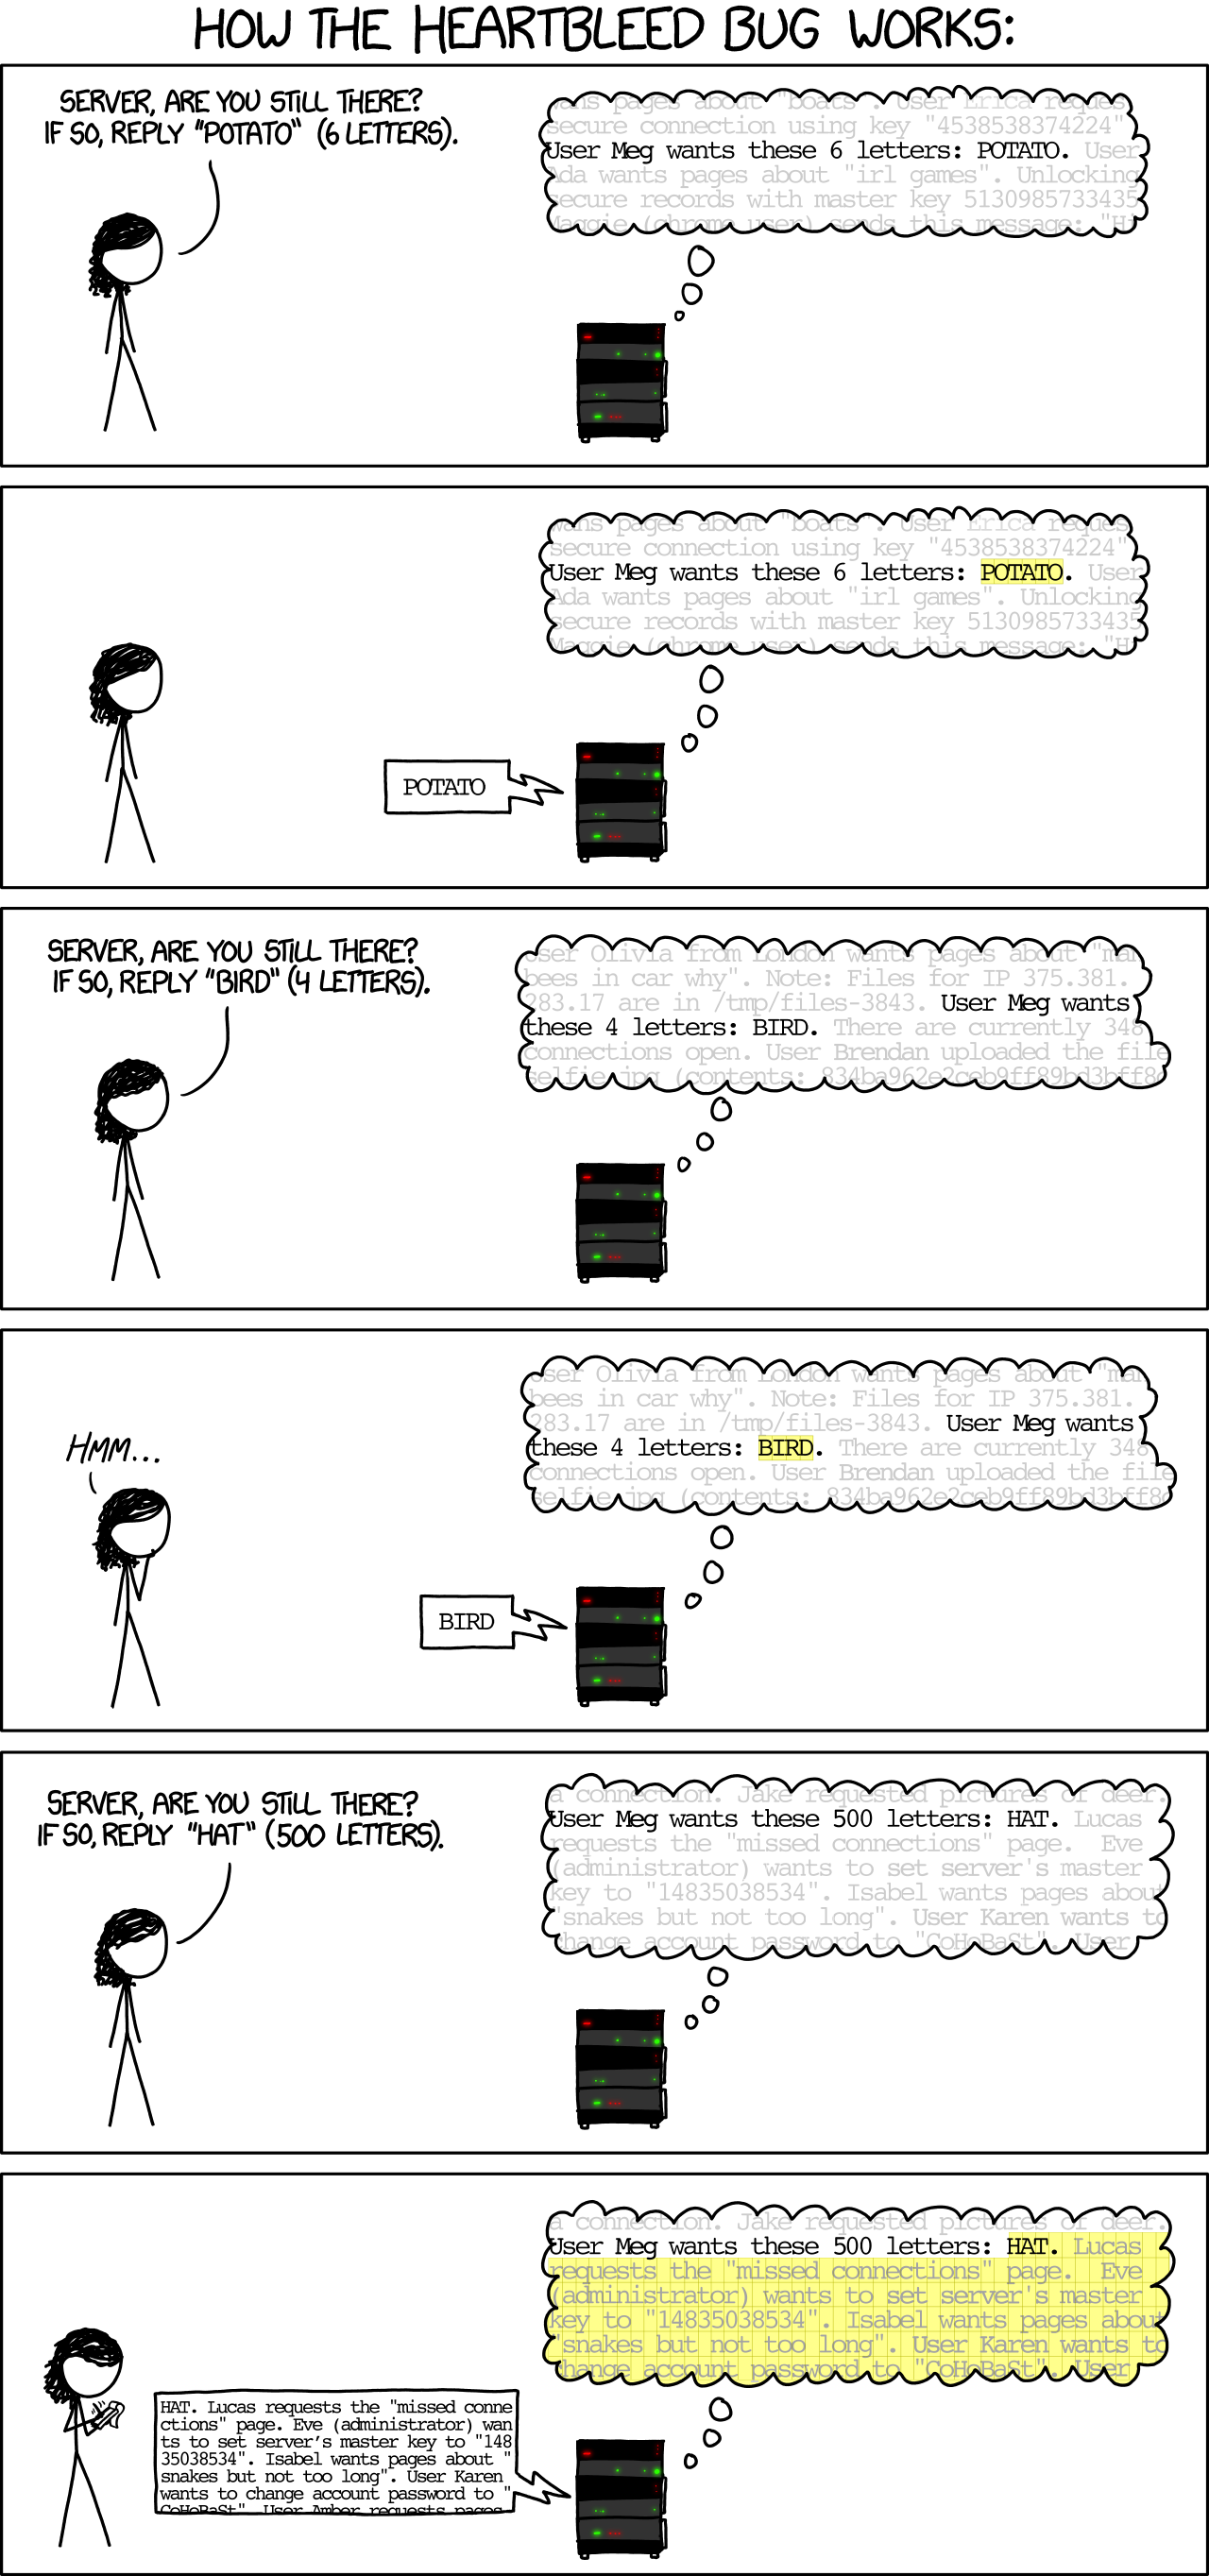
\includegraphics[scale=0.4]{comics/xkcd_heartbleed_explanation.eps}
\caption{XKCD \# 1353: Explanation of the Heartbleed Bug}
\end{figure}

When functions call other functions, each function gets its own chunk
of stack memory at the moment it is called;
it keeps all its local variables there, but also a program counter
that remembers where in its execution it was.
When the function finishes, its stack memory block is made available
for other purposes again.
For statically allocated variables,
the compiler can take care of all of this, and you typically don't
have to think about it.

\section{Scoping of Variables}
While we are talking about local variables and the stack, we should
briefly talk about the scope of a variable.
Global variables are, of course, accessible to any function or any
block of code in your program.
Local variables in functions or code blocks only exist while the
execution is in the function or the code block.
Local variables are typically stored on the stack.
As soon as the function or block terminates,
the variable is deallocated. 

When the execution of a function is temporarily suspended,
for instance because another function got called inside this one,
the variables are stored on the stack, but not active,
so they cannot be accessed.
Consider the following example:

\begin{verbatim}
void foo (int x)
{
  int y; 
  // do some stuff
}

void bar (int n)
{ 
  int m;
  foo (n+m);
  // do more stuff
}
\end{verbatim}

Here, when \code{bar} calls \code{foo}, the function \code{foo} cannot
access the variables \code{n} or \code{m}.
As soon as \code{foo} finishes, the variables \code{x} and \code{y}
are deallocated, and permanently lost.
\code{bar} now resumes and has access to \code{n} and \code{m},
but not to \code{x} or \code{y}.

You will sometimes have multiple variables (in different parts of your
code) sharing the same name.
For instance, you may have both a global variable \code{n} and a local
variable called \code{n} in a function.
Or you could have code like the following:

\begin{verbatim}
void foo (int n)
{
  int m = 10;
  // do something
  for (int i = 0; i < m; i ++)
    {
      int n = 3, m = 5;
      // do something
      cout << n << m;
    }
}
\end{verbatim}

Here, the \code{cout << n << m} statement would output the innermost
versions, so the values 3 and 5.
As a general rule, when there are multiple variables with the same name,
any reference is to the one in the smallest code block enclosing the
statement that contains that variable.
Of course, as another general rule, when you can, you should avoid
writing code that makes you and others think for a while to figure out
which variable is being referenced with a particular name.

\section{Dynamic allocation}
Static allocation works easily when the compiler can tell at compile
time how much memory will be needed.
However, in many cases, it is not known at compile time how much
memory a program (or particular structure within a program) needs.
As an example suppose that you want to do something like the following:

\begin{verbatim}
int n;
cin>>n;
// create an array a of n integers
\end{verbatim}

Here, at compile time, the compiler does not know how much memory the
array will need. It can therefore not allocate room for a variable on
the stack\footnote{Technically, this is not quite true. Some modern
  compilers let you define arrays even of dynamic sizes, but we advise
  against using this functionality, and instead do things as we write
  in these notes.}.
Instead, the program will need to explicitly ask the operating system
for the right amount of space at run-time. 
This memory is assigned from the \todef{heap}\footnote{This is called
  the heap space since it can be selected from any portion of the
  space that has not been allocated already. While the stack remains
  nicely organized, memory in the heap tends to be more messy and all
  over the place. Hence the name.} space. 

The difference between static and dynamic memory allocation is
summarized in the following table.
To fully understand how dynamic memory allocation works,
we need to spend some time on pointers.

\begin{table}[h]
	\centering
    \begin{tabular}{l|l}
       \textbf{Static allocation}         & \textbf{Dynamic allocation}                \\ \hline
        Size must be known at compile time & Size may be unknown at compile time \\
        Performed at compile time & Performed at run time             \\ 
        Assigned to the stack     & Assigned to the heap              \\ 
        First in last out         & No particular order of assignment \\
        Compiler takes care of deallocation & You must take care of
                                              deallocation \\
    \end{tabular}
\caption{Differences between statically and dynamically allocated memory.}
\end{table}

\section{Pointers}
A pointer is an ``integer'' that points to a location in memory ---
specifically, it is an address of a byte\footnote{This means that all
pointers are of the same size, and that the size of a pointer used by
a computer places a limit on the size of memory it can address.
For example, a computer using typical 32-bit pointers can only use up to
$2^{32}$ bytes or $4$ gigabytes of memory.
The modern shift to 64-bit architectures turns this to $2^{64}$ bytes,
which will be enough for a while.}. 

In C/C++, pointer types are declared by placing a star `*' behind a
regular type name.
Thus, \code{int *p; char *q; int **b; void *v;} all declare pointers.
In principle, all of these are just addresses of some memory location,
and C/C++ does not care what is stored at the address.
Declaring them with a type (such as \code{int}) is mostly for the
programmer's benefit:
it often prevents you from messing up the use of the
data stored in the location.
It also affects the way some arithmetic on memory locations is done,
which we will see below.

Two of the ways in which ``regular'' variables and pointers often
interact are the following:
\begin{enumerate}
\item You want to find out where in memory a variable resides, i.e.,
  get the pointer to that variable's location.
\item You want to treat the location a pointer points to as a variable,
  i.e., access the data at that location, by reading it or overwriting
  it.
\end{enumerate}
The following piece of code illustrates some of these, as well as
pitfalls one might run into.

\begin{verbatim}
int* p = nullptr, *q;	//Pointers to two integers
int i, j;
i = 5; j = 10;
p = &i;	  //Obtain the address of i and save it to p
cout << p;  //Prints the value of p (address of i)
cout << *p; //Prints the value of the integer that p points to (which is the value of i)
*p = j;   // Overwrites the value of the location that p points to (so, i) with the value of j
*q = *p;  // Overwrites the value of the location that q points to with the one that p points to
q = p;    // Overwrites the pointer p with q, so they now point to the same location
\end{verbatim}

A few things are worth noting here.
\begin{enumerate}
\item The last two commands both result in \code{*p} being equal to
\code{*q}, but in different ways. In the first case, we copy the
\emph{value} from one location to the other, while in the second, 
we make both point to the same place.
This will manifest itself later: if you make a change to \code{*p}
after writing \code{q = p}, it will also change \code{*q};
this does not happen if you wrote \code{*q = *p}.
\item In our code example, the second-to-last command is very risky,
  and will likely cause a run-time error.
  The piece of code did not initialize \code{q},
  so it points to an arbitrary memory location, quite possibly location 0.
  The code is trying to overwrite this location,
  which most likely the program is not allowed to do.
  The location may belong to the operating system or
  some other program\footnote{Fortunately, nowadays, all that happens
    is that your program throws a run-time error. In the past, the OS
    would often allow you to do such an overwrite, in which case often
    some complete system crashes would happen.}.
\item \code{nullptr}\footnote{\code{nullptr} was introduced in
    C++11. You will need to use the C++11 flag in order to be able to
    use this keyword. In older versions, the keyword used was
    \code{NULL}, which still works in later versions.} is a special
  pointer, typically used to express that a pointer is ``not pointing
  anywhere.'' Of course, it is actually pointing somewhere.
  \code{nullptr} is basically just another name for the number 0.
  But since your code should never access memory location 0,
  having this as a ``not initialized'' value is a useful convention.
\item Our earlier comment about the perils of
  uninitialized pointers suggests that whenever you have a pointer
  variable, you always assign it \code{nullptr} right away as you declare
  it. In our example, we did that for \code{p}, but should also have
  done the same for \code{q}.
  That way, if you later forget to assign it a memory location before
  dereferencing it, at least, it will cause a crash of your program,
  rather than possibly processing some garbage that it reads from the
  location.
  This is good coding practice to reduce your debug time.
\item \code{\&} and \code{*} are \emph{inverses} of each other.
  Thus, \code{\&*p} and \code{*\&p} are the same as \code{p}.
  (The exception is that \code{\&*p} throws a runtime error when applied
  to \code{p==nullptr}, instead of being equal to \code{p}.)
\end{enumerate}

In general, it is quite easy to mess up with pointers.
A few rules of thumb will weed out common mistakes,
but generally speaking, even experienced programmers produce runtime
errors frequently when dealing with pointers.

\begin{figure}[htb]
\centering
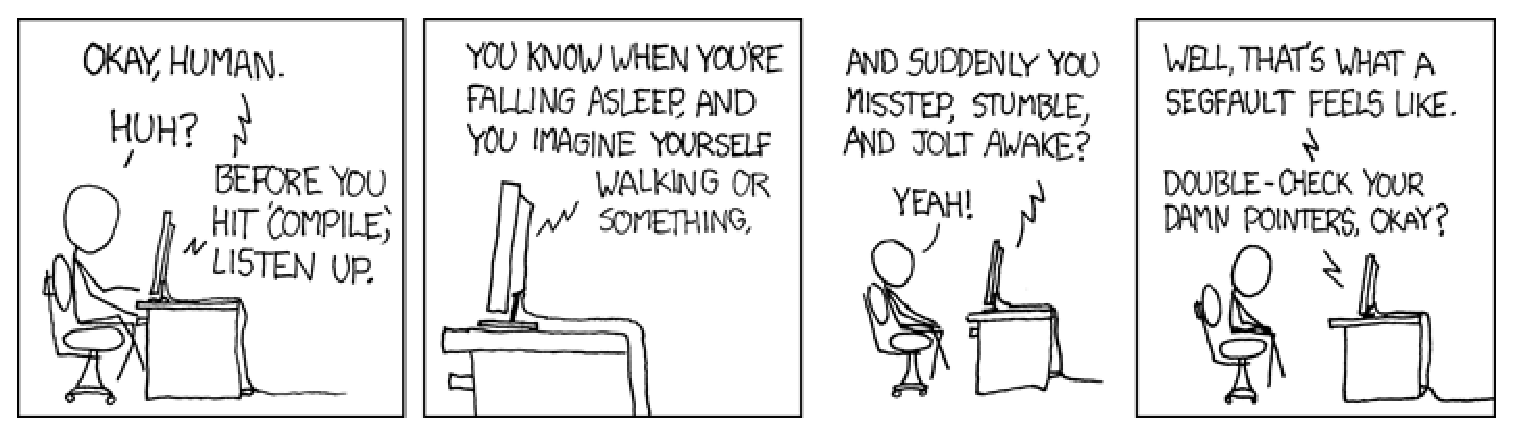
\includegraphics[scale=0.6]{comics/xkcd_compiler_complaint.eps}
\caption{XKCD \# 371: Check your Pointers!}
\end{figure}


We discussed before that pointers are basically just integers.
They differ in that arithmetic is somewhat different.
When you have a pointer \code{p} to an \code{int},
and you write \code{p+1},
the compiler assumes that what you want is the address
where the next \emph{integer} will start, which is 4 bytes later.
Thus, the actual address referenced by writing \code{p+1} is actually
4 bytes after the address of \code{p}.

This is where the type of pointer matters, as we mentioned above. 
When you have a \code{void*}, then addition really does refer to
adding individual bytes. For all other pointer types, when you write
\code{p+k} for a pointer \code{p} and integer \code{k}, 
this references memory location \code{p+k*size(<type>)}, where
\code{<type>} is the type of the pointer \code{p}.

\section{Dynamic Memory Allocation}
In order to dynamically allocate and deallocate memory,
C++ uses the functions \code{new} and \code{delete}.
They are built on the C functions \code{malloc} and \code{free},
which you can read about in Section~\ref{sec:dynamic-memory:malloc-free}.
The C++ versions shield you from some of the internals and will help
you avoid common mistakes in dealing with dynamic memory.

\subsection{C++ Style}
In C++, you allocate dynamic memory with \code{new()}
and deallocate it with \code{delete()}.
Let us look at allocation of memory first.
To solve our small problem from earlier --- ask the user for an array
size and allocated that much memory --- we would write the following:

\begin{verbatim}
int n;
int *b;
cin >> n;
b = new int[n];
for (int i=0; i<n; i++)
    cin >> b[i];
\end{verbatim}
The desired number of \code{int} spaces in the array is given in
square brackets, as with statically allocated arrays.

If we wanted space for just one integer, we could write
\code{int *p = new int;}
While this is not really very useful for a single integer,
it will become very central to allocating objects later,
where we often allocate one at a time dynamically.

When you allocate a single object, you can optionally give it a
default value in parentheses, as follows:
\code{int *p = new int (42); }
This code dynamically allocates a pointer to an integer,
and initializes the memory location's value to 42.
We will see later (in Sections~\ref{sec:classes:constructors} and
\ref{sec:overloading:copy-constructors}) that this is a special case
of copy constructors.

Another thing to observe here is that we can reference \code{b} just
like an array, and we write \code{b[i]}.
The compiler treats this exactly as \code{*(b+i)}, and, as you
probably remember from the part about pointer arithmetic, this points
to the \Kth{i} entry of the array.
In fact, that's exactly how C/C++ internally treats all arrays anyway;
basically, they are just pointers.

If we wanted to write \code{b[i]} in a complicated way by doing all
the pointer arithmetic by hand, we could write instead
\code{*((int*) ((void*) b + i * sizeof(int)))}.
Obviously, this is not what we like to type (or have to understand),
but if you understand everything that happens here, you are probably
set with your knowledge of pointer arithmetic and casting.

\smallskip

To release memory, we use the \code{delete} operator, as follows:
\begin{verbatim}
delete [] b;
delete p;
\end{verbatim}
The first example deallocates an array,
while the second deallocates a single instance of a variable
(a single \code{int} in our earlier example).
``Deallocating'' means that your code tells the operating system that
it won't need the memory at \code{p} any more, and the operating
system should feel free to reuse it for other purposes.

Note that \code{delete} does nothing to the pointers \code{b} or
\code{p} themselves;
it only deallocates the memory that they pointed to.
Thus, it is very good programming practice to immediately set the
pointer to \code{nullptr} after deallocating the memory it points to;
this way, your code will not attempt to tamper with invalid memory.

What could happen otherwise is the following:
you returned the memory to the operating system, which used it for
another variable (in your program or maybe another program).
Now you may accidentally overwrite or read the value that was written
into this new variable. Such a bug will be very hard to diagnose.
If you instead set the pointer to \code{nullptr}, you will instead get
a runtime error when you try to access the memory,
which is typically much easier to pin down and debug.

\subsection{C Style Memory Allocation (*)} \label{sec:dynamic-memory:malloc-free}
While we use C++ in this class, it is useful to understand the C-style
memory allocation as well.
After all, the C++ functions are built on top of the C ones,
and the C style is closer to the machine level, providing you perhaps
with a better understanding of what goes on inside your machine.

To allocate memory in C, one uses the function
\code{void* malloc (unsigned int size)}.
This function requests \code{size} bytes of memory from the operating
system, and returns the pointer to that location as a result. 
If for some reason, the OS failed to allocate the memory
(e.g., there was not enough memory available),
\code{nullptr} is returned instead.

The main difference between \code{malloc} and \code{new},
besides small syntax issues (square brackets for \code{new}
vs.~parentheses for \code{malloc}), is that when using \code{malloc},
you have to specify the number of \emph{bytes} you would like,
whereas with \code{new}, you specify the number of \emph{items} in
your array. 
This means that we need a way to figure out how many bytes will be
required for the number of items we want.
The way to find this out is the \code{sizeof} function.
When you write \code{sizeof (t)}, it returns the number of bytes for
each item of type \code{t};
for instance, \code{sizeof (int)} will give you the number of bytes in
an integer.
Even if you think that you know how many bytes a type will need,
you should never hard-code that constant, as it may change over time.
Even if right now, on your current computer, an integer needs 4 bytes,
that may not be the case forever if you reuse your code later.

Another difference between \code{malloc} and \code{new} is that
\code{malloc} returns a \code{void*},
since it does not know what kind of data we want to store at the
location.
As a result, we have to cast the pointer to the type that we want in
the end, for instance, an \code{int *}.
Taken together, the code we had earlier is therefore written as:

\begin{verbatim}
int n;
int* b;
cin >> n;
b = (int*) malloc(n * sizeof(int));
\end{verbatim}

For good coding practice, we should probably also check whether
\code{b==nullptr} before dereferencing it,
but this example is supposed to remain short.

\smallskip

The analogue to \code{delete} in C++ is the function 
\code{void free (void* pointer)};
it releases the memory located at \code{pointer} for reusing.
So our earlier code for releasing memory would now become

\begin{verbatim}
free (b);
free (p);
\end{verbatim}

Just like \code{delete}, the function \code{free} does not change the
pointer (\code{b} or \code{p}) and only deallocates the memory.
So as with \code{delete}, it is good coding practice to set the
pointers to \code{nullptr} (or, in C, \code{NULL}) after they are
deallocated.


\section{Memory Leaks}
Let us look a little more at the things that can go wrong with dynamic
memory allocation.

\begin{verbatim}
double *x;
...
x = new double [100];
...
x = new double [200]; // We're gonna need a bigger array!
...
delete [] x;
\end{verbatim}

This code will compile just fine, and most likely will not crash,
at least not right away.
We correctly allocate an array of 100 \code{double},
use it for some computation,
and then allocate an array of 200 \code{double} when we
realize that we need more memory.

But notice what happens here.
The moment we do the second allocation, \code{x} gets overwritten with
a pointer to the newly allocated memory block.
At that point, we have no more recollection of the pointer to
the previous memory block.
That means we cannot read it, write it, or deallocate it.
When at the end of the code snippet,
the program calls \code{delete [] x},
it successfully deallocates the second allocated block,
but we are unable to tell the operating system that we do not need the
first block any more. 
Thus, those 800 bytes will never become available again
(until our program terminates --- but for all we know, it may run for
several years as a backend server somewhere).

This kind of situation is called a \todef{memory leak}:
available memory is slowly leaking out of the system.
If it goes on long enough, our program may run out of memory and crash
for that reason. It could be quite hard to diagnose why the crash
happened if it does after a long time of running.

It is good practice to keep close track of the memory blocks you
reserve, and make sure to \code{delete} (or \code{free}) memory
pointed to by a pointer before reusing the pointer\footnote{There are tools
for checking your code for memory leaks, and we recommend
familiarizing yourself with them. The most well-known one, for which
the course web page contains some links, is called \code{valgrind}.}.
A better version of the code above would be the following:

\begin{verbatim}
double *x;
...
x = new double [100];
...
delete [] x;
x = nullptr;
x = new double [200];
...
delete [] x;
x = nullptr;
\end{verbatim}

That way, the memory gets released while we still have a pointer to
it.
You will recall that it is always good practice to immediately set
pointers to \code{nullptr} after deallocating their memory.
In the middle of the code, that may seem very redundant:
after all, the example program immediately overwrites \code{x} with
another value. 
And in fact, here, it \emph{is} completely redundant.
However, we still recommend that you add the line;
for example, you may later insert some code between \code{delete [] x}
and \code{x = new double [200]}, and you might easily insert mistakes there.
And if you are worried about your program wasting time with
unnecessary assignments, don't be --- the compiler will almost certainly
optimize that assignment away anyway, and the final compiled code will look
exactly the same.

One question you may be wondering about is if we could just free the
memory by setting \code{x = nullptr;}
without calling \code{delete [] x} first.
That would only overwrite the pointer, but it would not tell the
operating system that it can have the memory back.
In other words, it would exactly \emph{create} a memory leak.
Whenever you want to return memory to the system, you must do so
explicitly\footnote{There are other programming languages that do much
  more of the garbage collection and memory handling for you,
  but C/C++ is not one of them.}. 

As a side note, if you look up some of this information online or in
other sources, keep in mind that the pool of memory where you allocate
variables with \code{new} (or \code{malloc}) is called the
\todef{memory heap}.
This is different from a data structure known as the \emph{heap} which
you will learn about in Chapter~\ref{chap:priority-queues}.
Unfortunately, people (including us $\ldots$) are not quite consistent
in naming these.

%\section{Exercises}

\subsection{\ReviewQuestions}

\begin{exercise}
  What is the difference between stack and heap memory?
  As a general rule, what is stored on the stack and what is stored on
  the heap?
\end{exercise}

\begin{exercise}
  When you have two variables of the same name \code{x} in a block of code,
  which one is accessed when you refer to \code{x}?
\end{exercise}

\begin{exercise}
  Describe what the operators \code{*} and \code{&} do.
\end{exercise}

\begin{exercise}
  Why can the compiler not always determine all memory requirements at
  compile time?
\end{exercise}

\begin{exercise}
  Besides your program's variables/data, what else is stored in
  memory on your computer? What is stored in the stack memory when
  your program runs (besides local variables)?
\end{exercise}

\begin{exercise}
  What could happen when you try to read/write a memory location that
  does not belong to your program?
\end{exercise}

\begin{exercise}
  Why is it a good idea to initialize all your pointers to
  \code{nullptr} when you declare them
  (unless you already know what value they need to take)?
\end{exercise}

\begin{exercise}
  What is it called when you dynamically allocate memory but do not
  deallocate it? Why can this be a problem?
\end{exercise}

\begin{exercise}
  Why should you not assume a fixed number of bits/bytes for the
  length of an integer or double?
\end{exercise}

\begin{exercise}
  Why should you always set a pointer to \code{nullptr} after
  deallocating its memory?
\end{exercise}

\subsection{\EasyQuestions}

\begin{exercise}
  What is the difference between \code{int *p = new int (5);}
  and \code{int *p = new int [5];}?
\end{exercise}

\begin{exercise}
  Suppose that you have a variable \code{int *p}, which happens to be
  stored in location 100.
  Which memory location is accessed when you write
  \code{p+1}?
  How about when you write \code{(void*) p + 1}?
\end{exercise}

\begin{exercise}
  In the following code, will all the allocated memory be correctly
  deallocated? Why or why not?
\begin{verbatim}
  int *p = new int [50];
  for (int i = 0; i < 50; ++i)
     p[i] = i;
  p = nullptr;
\end{verbatim}
\end{exercise}

\subsection{\MediumQuestions}
\begin{exercise}
  Fill an array with numbers, read between array positions.
\end{exercise}

\subsection{\HarderQuestions}
\begin{exercise}
  Skyskraper
\end{exercise}

%%%%%%%%%%%%%%%%%%%%%%%%%%%%%%%%%%%%%%%%%%%%%%%%%%%%%%%%%%%%%%%%%%%
\chapter{Strings and Streams: A Brief Review}
\label{chap:strings-streams}
[Note: This chapter covers material of about 0.25 lectures.]

%As part of solving various assignments,
you will frequently need to read and process strings,
and input and output in C++ are typically handled using streams.
While you should have learned these in your introductory programing
class, we will give a brief review here, focusing on issues that seem
to often cause students difficulties.
You can look up exact syntax in your introductory C++ textbook or
online.

\section{Strings}
In basic C, string are implemented just as arrays of characters. 
There is no separate string type. 
This means that you need to allocate enough space for your character
array to hold any input string that you might receive.
It also means that you need a special way of marking how much of that
array you are \emph{actually} using: just because you allocated, say,
80 characters in your string does not mean you will always use all 80.
The way C does this is by having a special role for the character
\code{\textbackslash{}0}.
(That's the character number 0, not the actual character `0'.)
It marks the end of the used part of the string.

The \code{string} class in C++ is a little easier to use:
in particular, it hides some of the memory management for you,
so that you don't have to worry about allocating enough space.
It also implements some operators that you will frequently use, such
as \code{=} (assignment), \code{==} (comparison) and \code{+}
(appending strings). 
The \code{string} class also contains a number of other very useful
functions. Since you will be doing a lot of processing of data you are
reading in from files in this class, you can probably save yourself a
lot of work by reviewing the \code{string} class and its features.

One string function which is really useful in C,
but to our knowledge does not have an equivalent in C++ in standard
implementations, is \code{strtok}.
It allows you to tokenize a string, i.e., break it into smaller chunks
using any set of characters as separators.
Check it out!

\section{Streams}
Streams are the C++ ways of interacting with files, keyboard, screen,
and also with strings.
There are streams you read (keyboard, files, strings)
and streams you write (screen, files, strings).
In all cases, they are basically a sequence of characters
that you are extracting from (read) or inserting into (write).
They are a fairly clean abstraction of reading and writing ``items''
one by one.

The standard streams you will be interacting with are given in
Table~\ref{tab:streams}. 
They require you to \code{\#{}include} different header files, also
listed here.

\begin{table}[htb]
\begin{tabular}{l|l|l}
Stream & Target & Header File \\ \hline
\code{cin} & Keyboard & \code{iostream} \\
\code{cout}, \code{cerr} & Screen & \code{iostream} \\
\code{ifstream} & File to read & \code{fstream} \\
\code{ofstream} & File to write & \code{fstream} \\
\code{stringstream} & String & \code{sstream} \\ \hline
\end{tabular}
\caption{The streams you will use most frequently.\label{tab:streams}}
\end{table}

The difference between \code{cout} and \code{cerr} is twofold:
First, \code{cout} buffers its output instead of printing it immediately,
whereas \code{cerr} prints immediately. 
This makes \code{cerr} very useful to output debug information,
whereas you will probably write your ``real'' output to \code{cout}.
They are also two different logical streams. This means that if you
redirect your output to a file (which we will do when grading you),
the default is that only \code{cout} gets redirected.
So if you print debug information to \code{cerr},
it still appears on the screen, and doesn't ``pollute'' your output. 
Finally, \code{cerr} often gets displayed in a different color.
All this is to say: it may be good to get into the habit to print all
your ``real'' output to \code{cout},
and all of your debug output to \code{cerr}.

To extract items from an input stream, you use the \code{>>} operator,
and to insert items into an output stream, you use \code{<<}.

A few things are worth remembering about reading from an input
stream. (These frequently trip students up.)
\begin{itemize}
\item When reading from a stream (say, \code{cin}, or a \code{ifstream
    myinput}), you can use \code{cin.fail()} (or \code{myinput.fail()})
  to check whether the read succeeded.
  When one read fails (and the \code{fail} flag is set), it will
  remain set until you explicitly reset it with \code{cin.clear()} or
  \code{myinput.clear()}. Until then, all further reads will fail,
  since C++ assumes that until you have fixed the source of the problem,
  all incoming data will be unreliable now.

\item Remember that \code{>>} reads until the next white space, which
  includes spaces, tabs, and newlines.

  Be careful here when entering things manually. If at the first
  prompt, you enter multiple items separated by space, they will
  ``supply'' the next few extractions. That is, if you write code like
\begin{verbatim}
cout << "Please enter n:"
cin >> n;
cout << "Please enter m:"
cin >> m;
\end{verbatim}
  and enter ``5 3'' at the first prompt, it will read 5 into \code{n}
  and 3 into \code{m}.
  In particular, this is likely to trip you up if you somehow try to
  read an entire line of text from a file using \code{>>}, and that
  line happens to contain white spaces.

\item If you want to also read spaces, then instead of using
  \code{>>}, you should use \code{getline}, such as
  \code{cin.getline()} or \code{myinput.getline()}. 
  It lets you specify a string to read into, 
  a maximum number of characters to read, and 
  character to stop at (default is newline), and will then read into
  the string. That string can later be further processed.

  Notice that you need to be a bit careful about \code{getline} at the
  end of a file; you may need to check the correct flags to avoid reading the
  last line multiple times.

\item If you want to ``clear'' off the remaining characters in a
  stream so they don't cause issues later, you can use the
  \code{ignore (int n)} function, which will ignore the next \code{n}
  characters (which you can specify --- default is 1).
\end{itemize}

\subsection*{File Streams and String Streams}
File streams are the typical C++ way of reading data from files.
The two types are \code{ifstream} (for files you read) and
\code{ofstream} (for files you write).
A file stream needs to be opened before you can read/write from it. 
Once you have opened it, it can basically be used like \code{cin} and
\code{cout}.

Notice that in file streams, when you read \emph{over} the end of the
file, you will get a \code{fail} condition.
That happens after you \emph{reach} the end of the file,
which is often cause for confusion when using \code{getline}.

The other thing to keep in mind about file streams is that after
you are done, you should call \code{close()} on them.

\medskip

Since strings are sequences of characters, just like files,
it is natural to treat them as streams as well.
This is what the \code{stringstream} type is for.
It is particularly useful when you have read an entire string and want
to break it into smaller pieces, e.g., separated by spaces.
You can treat the string as a \code{stringstream}, and then use extraction
operations on it to get the different items.
This is also a convenient way to convert strings to integers.

As a piece of advice, avoid using the same \code{stringstream} object
multiple times --- or if you do, you must make sure to reset it.
% \section{Exercises}

\subsection{\ReviewQuestions}
\begin{exercise}
  What is meant by string tokenization, and what is it good for?
\end{exercise}

\begin{exercise}
  What is the difference between the C++ \code{string} class and the
  way in which C handles strings?
\end{exercise}

\begin{exercise}
  What are the differences between \code{cout} and \code{cerr}?
  Typically, when would you use which one?
\end{exercise}

\begin{exercise}
  When would you use \code{getline} vs.~\code{cin >> myString}?
\end{exercise}

\subsection{\EasyQuestions}

\begin{exercise}
  Suppose that you have a file \code{myFile.txt} that contains just the line
\begin{verbatim}
Data Structures is my favorite subject.
\end{verbatim}
  and you execute the code
\begin{verbatim}
ifstream myFile ("myFile.txt");
string line;
myFile >> line;
\end{verbatim}
  What will be the content of \code{line} at the end?
\end{exercise}

%%%%%%%%%%%%%%%%%%%%%%%%%%%%%%%%%%%%%%%%%%%%%%%%%%%%%%%%%%%%%%%%%%%
\chapter{Recursion}
\label{chap:recursion}
[Note: this chapter covers material of about 1.5 lectures.]

%The adjective \todef{recursive} means ``defined in terms of itself.''
As computer scientists, we frequently run into recursion in the form
of recursive functions, which are functions that call themselves
(directly, or indirectly through another function).
However, as we see below, another very important
application is recursive definitions of objects.
We will explore recursion through several examples.

\begin{figure}[htb]
\centering
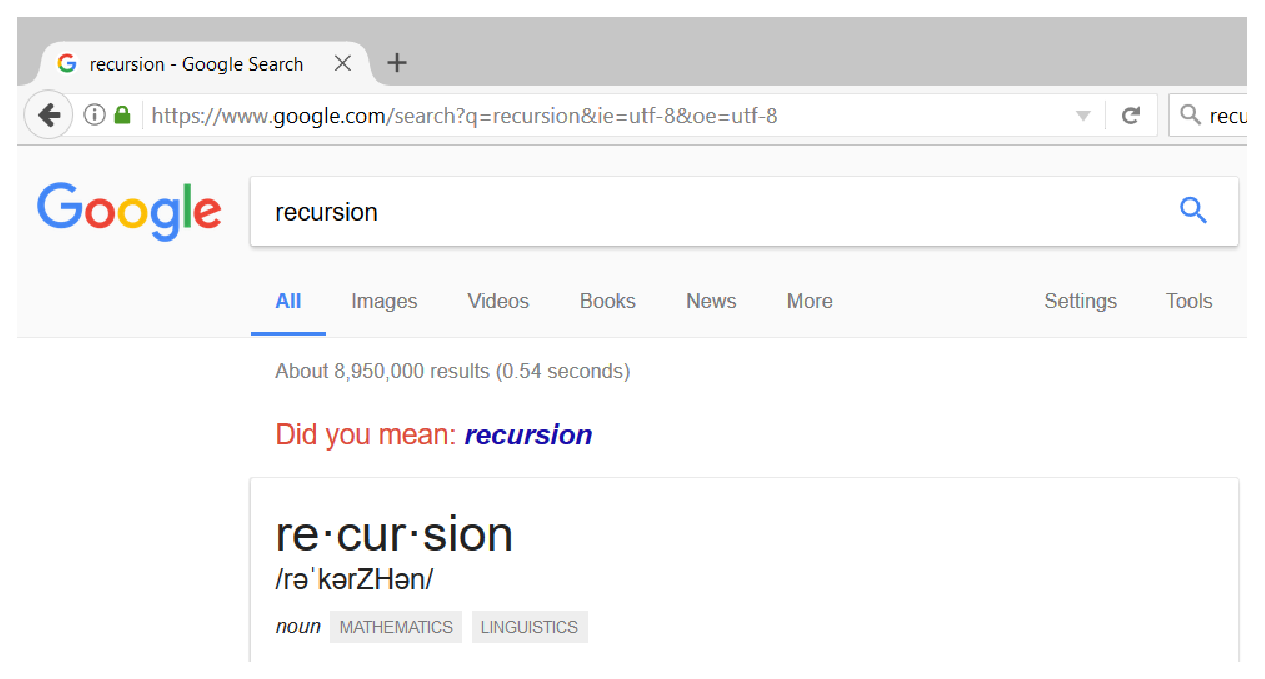
\includegraphics[scale=0.6]{comics/recursion-screenshot.eps}
\caption{What happens when you Google ``recursion''}
\end{figure}


\section{Computing Factorials}
Our first example, which you have likely seen before,
is to compute the factorial of $n$, which is defined 
as $n! = n \cdot (n-1) \cdot (n-2) \cdots 2 \cdot 1 = \prod_{i=1}^n i$.
Of course, we could use iteration (a simple \code{for} loop) to
compute $n!$.
\begin{verbatim}
int factorial(int n) {
    int p=1;
    for (int i=1; i<=n; i++)
        p*= i;
    return p;
}
\end{verbatim}

This is a perfectly valid, and probably even the best,
way to compute the factorial of a number.
However, in this section, we will use this very easy example
to illustrate how recursion works.

Looking at the definition, we observe that $0! = 1$ (by definition),
and $n! = n \cdot (n-1)!$.
This suggests a recursive solution for computing factorials:

\begin{verbatim}
int factorial (int n) {
    if (n==0) return 1;
    else return n*factorial(n-1);
}
\end{verbatim}

Notice that the function \code{factorial} calls itself;
this is what makes our implementation recursive.
Many students have trouble thinking about recursion initially.
Our instinct is often to make a complete plan for the computation:
first multiply $n$ with $n-1$, then with $n-2$, and so on,
all the way to $1$. 
In a recursive solution, we instead treat most of the work as a
``black box:'' we do not really worry \emph{how} the call with
parameter $n-1$ will obtain the correct results, and just trust
\emph{that} it does.
Of course, that only works if the function is actually correct,
but since you yourself are writing the function, you can make sure
that the outcome will be correct \emph{assuming} that what you got
from the recursive call was correct.

To illustrate this concept in even more detail, consider computing
$n!$ with a group of classmates.
Each student is in charge of computing the value $n!$ only for one
particular number $n$.
The student in charge of computing $5!$ relies on another student to
compute $4!$, then uses her result and multiplies it with 5.
So we get a long chain of work delegation,
where every student only carries out one multiplication
and relies on another student for all the preceding work.
The important insight here is that the student who must compute
$5!$ does \emph{not} need to know how the other student computes $4!$;
so long as the $4!$ student got the right result,
it can just be plugged in.
Maybe the $4!$ student used a loop instead of recursion?
Or maybe she is just really good at guessing factorials.
It does not matter to the $5!$ student --- so long as the result is
right, he can use it.

To recap this once more, in a recursive solution,
we do not have to think of every step,
nor do we have to keep track of various intermediate results,
as those are returned as values by the other function calls. 
Students getting started on recursion often try as hard as possible to
have recursion emulate loops, by passing around ``global variables''
(or pointers to variables, which amounts to the same thing)
that are altered and store intermediate results.

This type of thinking can take a while to get used to,
but once you firmly grasp it, a lot of things
--- most importantly induction and, later on, dynamic programming ---
will come to you much more easily.

Two things that pretty much all correct recursive functions share are
the following:

\begin{itemize}
\item A recursive function needs one or more base case: at some point,
  the function must hit a point where it will no longer call itself
  (like the \code{n==0} case for the factorial). 
  Otherwise, the function will keep calling itself forever, and
  eventually run out of stack memory.
\item Recursive calls must have ``smaller'' inputs than the main
  input. In the case of the \code{factorial} function, the recursive
  call within \code{factorial(n)} was for \code{factorial(n-1)}.
  In this case, it is clear that $n-1$ is ``smaller'' than $n$.
  In other cases, ``smaller'' refers to the remaining size of an
  array, or even a number that is closer to an upper bound.
  (For instance, the base case could be \code{i==n}, and the call with
  input $i$ could be to $i+1$.)
\end{itemize}

Let us look quickly at two examples violating these conditions, and
see what happens.

\begin{verbatim}
int UCLAfact (int n) // apologies to our neighboring school
{
   if (n == 0) return 1;
   else return UCLAfact (n); // error: input not getting smaller!
}

int NDfact (int n)
{
   return n*NDfact (n-1); // ...this doesn't stop!
}
\end{verbatim}

Neither of these functions will terminate.
In the first example, we do have a base case, but the recursive call
has the same size.
It is of course correct that $n! = n!$
(which is what the function uses),
but it doesn't help us compute it.
In the second example,
we do have a smaller input in the recursive call,
but no base case, so the function will continue calling itself
with different values forever
(or until it runs out of stack space and crashes).

\begin{figure}[htb]
\centering
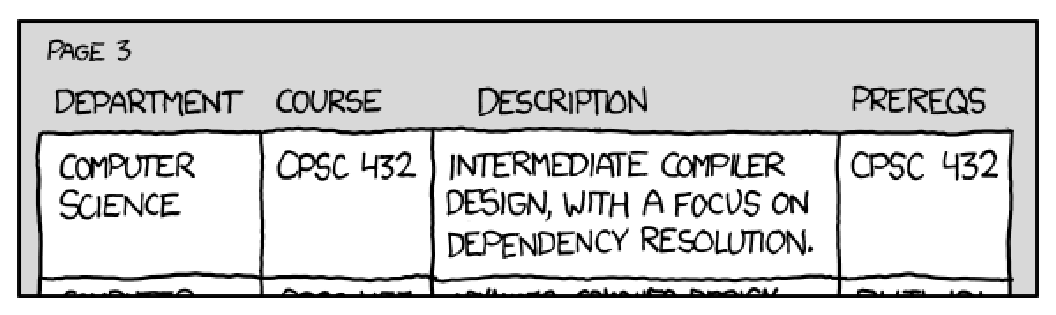
\includegraphics[scale=0.6]{comics/xkcd_dependencies.eps}
\caption{XKCD \# 754: Recursive Course Dependencies}
\end{figure}

\section{Binary Search}
Admittedly, computing factorials is not a very strong example to show
why recursion is useful, since the iterative solution is short and
elegant. However, we were able to illustrate some of the important
properties of recursion with an easy enough general setup.
Next, let us look at a somewhat more challenging task:
Given a (pre-sorted) array of integers in increasing order, find the
location of a target element, or return -1 if it is not in the array.
(If instead of integers, our array contained the names of students in
the class, we would have the setting we looked at in
Example~\ref{exm:overview:binary-search}.)

This task is accomplished using the \todef{Binary Search} algorithm:
Check the middle of the remaining array.
If the element is there, we are done.
If the desired element is smaller,
continue searching to the left of the middle element;
otherwise, continue searching to the right.
A corresponding iterative solution looks as follows:

\begin{verbatim}
int binarySearch (int n, int* b, int len) 
{
   int lo = 0, hi = len, mid;
   while(lo <= hi) {
       mid = (hi+lo)/2;
       if (b[mid]==n) return mid;
       else if(n < b[mid])
                 hi = mid-1;
            else lo = mid+1;
    }
    return -1;
}
\end{verbatim}

A recursive solution looks as follows:

\begin{verbatim}
int recSearch(int n, int* b, int lo, int hi) {
    if (hi < lo) return -1;  // not in the array
    else 
      {
        int mid = (hi+lo)/2;    // the midpoint of the array
        if (n == b[mid]) return mid;    // we found it
        else if (n < b[mid]) 
             return recSearch(n, b, lo, mid-1);  // element to the left of the midpoint
        else return recSearch(n, b, mid+1, hi);  // element to the right of the midpoint
      }
}
\end{verbatim}

To start the search, we call the function as \code{recSearch(n, b, 0, len)}.
Whether you like the iterative or the recursive solution better here
may be a matter of taste, but notice that there is a certain elegance
to the recursive solution.
When we have decided where the element must be (to the left or the right),
rather than updating a variable and repeating,
we simply ask the function to find it for us in that (correct) subarray,
and return its return value unchanged.
This is akin to delegating the task of finding the number in the
smaller array to another student, as we discussed earlier.

Notice that both implementations will work whether the array has an
even or odd number of elements.
If we hadn't written \code{mid-1} and \code{mid+1} for the recursive calls,
we might have needed another base case when \code{lo == hi}. 

Let us check that we satisfy the two conditions above for a recursive
solution to have a chance to work:
\begin{itemize}
\item If the array is empty (which is the case \code{hi < lo}),
  the function returns directly,
  reporting that the element was not found. 
\item If \code{n} is less than the midpoint,
  the function recurses on the left half of the array;
  otherwise, on the right half.
  In either case, because we eliminate at least the midpoint,
  the remaining array size is strictly smaller than before.
\end{itemize}

One of the things that can be confusing about recursion is that there
seem to be many ``active'' versions of the function at once.
What is ``the'' value of variables like \code{n}, \code{lo},
\code{hi}, or \code{mid}?
After all, different invocations of the function will have different
values for them.
To solve this ``conundrum,'' remember from our overview of memory that
local variables are stored on the stack, and translated into memory
locations by the compiler and OS.
Thus, when the function \code{recSearch(12,b,0,10)} calls
\code{recSearch(12,b,0,4)}, their variables \code{lo}, \code{hi}
translate to completely different memory locations.
When the call \code{recSearch(12,b,0,4)} executes,
the values are \code{lo=0, hi=4}, and \code{mid=2} will be computed.
In the call \code{recSearch(12,b,0,4)},
we instead have \code{lo=0, hi=10, mid=5}.
The computer has no problem with the same variable name,
as only one meaning of the variable is in scope at a time.

\section{Enumerating all Binary Strings of a given length}
The first two examples we saw were pretty easily coded with a simple loop.
In general, if you have a recursive function that uses just one
recursive call to itself, it is often easily replaced by a loop.
Recursion becomes much more powerful
(as in: it lets you write short and elegant code for problems that
would be much more messy to solve without recursion)
when the function calls itself multiple times.

We will see several examples of that later in class with some clever
recursive sorting algorithms and other algorithms.
Another very common application is \todef{exhaustive search},
which is frequently based on enumerating all binary strings or strings
over some other set of letters (called ``alphabet'').
In turn, such an enumeration forms the basis of a technique called
``Backtracking.''

To derive a recursive solution for this problem,
let us return to our earlier thought experiment of students delegating
subtasks to each other.
Suppose that you have been asked to print all binary strings of length
3, but you can call on classmates who have expertise in printing
binary strings of length 2.
And you are lazy, so you would like to utilize this expertise to the
maximum.
Take a quick look at Table~\ref{tab:recursion:binary}.
It shows all binary strings of length 3,
arranged in a suggestive pattern.
Looking at the top part,
we see the digit `0' always in the first position, 
and followed by all binary strings of length 2.
Then, in the bottom part, we have the digit `1' in the first position,
followed again by all binary strings of length 2.

\begin{table}[htb]
\begin{tabular}{|c|c c|}
  \hline
  0 & 0 & 0 \\
  0 & 0 & 1 \\
  0 & 1 & 0 \\
  0 & 1 & 1 \\ \hline

  1 & 0 & 0 \\
  1 & 0 & 1 \\
  1 & 1 & 0 \\
  1 & 1 & 1 \\ \hline
\end{tabular}
\caption{The eight binary strings of length three. \label{tab:recursion:binary}}
\end{table}

So if you want to save yourself a lot of work, you could write `0' in
the first position, and then ask your classmate to fill in all the
strings of length 2 in the remaining positions
(and print the whole thing).
Then, when your classmate is done, you can overwrite your `0' with a
`1', and then ask the same classmate to repeat what he did earlier.

Of course, there was nothing specific about the numbers 3 and 2 here;
you could do the same thing for 42 and 41
(except we couldn't fit the example table in these notes).

Using the ideas we just worked out, we can now write down a recursive
algorithm.

\begin{verbatim}
void binaryStrings (int length, string s, int pos)
{
   if (pos == length) cout << s << endl;
   else
      {
        s [pos] = '0';
        binaryStrings (length, s, pos+1);
        s [pos] = '1';
        binaryStrings (length, s, pos+1);
      }
}
\end{verbatim}

In this piece of code, \code{length} is the length of the binary
strings you are trying to print,
\code{s} is the string you are building (with your classmates),
and \code{pos} is the position you personally are in charge of.
As we said above, you do your part by putting `0' in your position,
then delegating the rest of the task to your classmate in charge of
position \code{pos+1}.
Then, you put `1' in your position, and again delegate the rest to
your classmate in charge of position \code{pos+1}.
Notice a few things here:
\begin{itemize}
  \item The first call would be \code{binaryStrings (0, s, length)},
    where \code{s} is some string that we allocated to be of the given
    length.
  \item We chose our base case to be that \code{pos==length}, not
    \code{pos==0}.
    We could have done that, too (or maybe \code{pos==-1}),
    in which case we would need to replace \code{pos+1} with
    \code{pos-1} in the recursive calls.
  \item The ``size'' of the input to solve is measured as
    \code{length-pos} here; whenever a call happens with \code{pos+1},
    this size (how many more digits need to be filled in) gets
    smaller, and the program gets ``closer'' to the base case.
  \item There was nothing particularly special about the strings being
    binary. Enumerating numbers in any base, or printing strings over
    any alphabet, is an easy modification of the above code.
    (Hint: \code{for} loops might come in handy.)
\end{itemize}

Experience tells us that such code is often difficult for students to
understand at first.
We recommend going through it by hand for \code{length==3} and
\code{length==4} and keeping track of all recursive function calls and
their variables and where they are in their execution.

\section{The $n$-Queens problem (*)}
In the $n$-queens problem, you want to place $n$ queens on an 
$n \times n$ chessboard (square grid). 
Each queen occupies one square on a grid and no two queens share the
same square. Two queens are \emph{attacking} each other if one of
them can travel horizontally, vertically, or diagonally and hit the
square the other queen is on.
The problem is to place the queens such that no two queens are
attacking each other.
For instance, what you see in Figure~\ref{fig:queens} is not a legal
solution: the queens in columns 1 and 3 attack each other diagonally,
as do the the queens in columns 2 and 3.
(All other pairs of queens are safe, though.)

\begin{figure}[htb]
\begin{center}
\setlength{\unitlength}{1cm}
\begin{picture}(5,5)
\linethickness{0.02mm}
\multiput(0,0)(0,1){6}{\line(1,0){5}}
\multiput(0,0)(1,0){6}{\line(0,1){5}}
\large
\put(0.4,0.4){Q}
\put(4.4,1.4){Q}
\put(2.4,2.4){Q}
\put(1.4,3.4){Q}
\put(3.4,4.4){Q}
\end{picture}
\caption{Illustration of the 5-queens problem \label{fig:queens}}
\end{center}
\end{figure}

Before we try to solve the problem, we make some observations.
Because queens attack each other when they are in the same row or
column of the chessboard, we can phrase the problem equivalently as
follows: place exactly one queen per row of the board such that no two
queens are in the same column or attack each other diagonally.

Thus, each row has a designated queen, and for each queen,
the program needs to try all possible columns.
If we didn't also need to check the diagonals,
this would look very similar to the binary strings enumeration we just
saw.
Each of the $n$ rows is like a position in the binary string,
and the column of its designated queen is like the character we chose,
ranging also from $0$ to $n-1$.
To avoid having to pass around variables like \code{s} and
\code{length} in \code{binaryStrings}, we will assume that we have
global variables

\begin{verbatim}
int *q; // array for the positions of the queens
int n;  // size of the grid
\end{verbatim}

Adapting our earlier \code{binaryStrings} code, the basic scaffold of
our $n$-queens solution will look as follows:

\begin{verbatim}
void queenSearch (int row)
{
   if (row == n) printSolution (); // that function shows the layout
   else
      {
        for (q[row] = 0; q[row] < n; q[row]++)
           {
               queenSearch (row+1);
           }
      }
}
\end{verbatim}

This short piece of recursive code will try all combinations of
positions for the $n$ queens, for a total of $n^n$ ways of placing
the $n$ queens. 
However, so far, it prints everything, including illegal solutions;
we have to modify the code to not print solutions if two queens can
attack each other.
There are a few ways to do this, but perhaps the most intuitive is to
keep an array of size $n \times n$ of positions that are currently
threatened by one or more queen.
That way, we can avoid placing a queen in a threatened position in the
first place, which should be much faster than only checking at the
very end.
Doing this kind of early checking is often called ``Backtracking.''

To decide on what we need to store in the array, we can think ahead a
bit about how we will update the array.
When we place a new queen, we will need to mark everything it
attacks as ``threatened.''
Then, when we remove the queen later to try a different position,
we want to mark those positions as ``not threatened.''
But we have to be careful: if a position is threatened by two queens,
and we remove the second threat, the position is still threatened, so
we cannot mark it ``not threatened.''
So it turns out to be better to mark \emph{how many} currently placed
queens threaten each position.

This suggests that we want a 2-dimensional array of \code{int}.
We will call that array \code{int **t} (for ``threatened''),
and also make it a global variable.
Because it is a two-dimensional array, it needs to be a pointer to a
pointer, and we have to be careful to initialize it fully and allocate
the memory for it dynamically.
Using our new array \code{t} (which we need to initialize to all-0
outside the \code{queenSearch} function), the new version of
the recursive function looks as follows:

\begin{verbatim}
void queenSearch (int row)
{
   if (row == n) printSolution (); // that function shows the layout
   else
      {
        for (q[row] = 0; q[row] < n; q[row]++)
           if (t[row][q[row]] == 0)
           {
               addToThreats (row, q[row], 1);
               queenSearch (row+1);
               addToThreats (row, q[row], -1);
           }
      }
}
\end{verbatim}

The new code \code{if (t[row][q[row]] == 0)} only places a queen if
the current candidate column is not threatened.
Then, it adds one threat to all positions threatened by the queen we
just placed.
After the recursive call returns, the queen gets removed (and placed
somewhere else), so we subtract one threat from all positions it
reaches; hence the -1.
Notice that this code is very compact, and not too big of a deviation
from what we saw for enumerating all binary strings.
This elegance is frequently a feature of recursive Backtracking
solutions.

Now, basically all that remains is to write the function \code{addToThreats},
which increases the number of threats for the threatened squares.
The function should mark all places on the same column, and on the two
diagonals below the current square.
For the latter, we need to make sure not to leave the actual grid.
Looking at it a little carefully,
you will see that the following function does that:

\begin{verbatim}
void addToThreats (int row, int column, int change)
{
   for (int j = row+1; j < n; j++)
      {
         t[j][column] += change;
         if (column+(j-row) < n) t[j][column+(j-row)] += change;
         if (column-(j-row) >= 0) t[j][column-(j-row)] += change;
      }
}
\end{verbatim}

Finally, we need to write our \code{main} function that reads the
size, creates the dynamic arrays, initializes them, and starts the
search.

\begin{verbatim}
int main (void)
{
   cin >> n;
   q = new int [n];
   t = new int* [n];
   for (int i = 0; i < n; i++)
      {
        t[i] = new int [n];
        for (int j = 0; j < n; j ++)
            t[i][j] = 0;
      }
   search (0);
   delete [] q;
   for (int i = 0; i < n; i ++) delete [] t[i];
   delete [] t;
   return 0;
}
\end{verbatim}

If you do not yet fully understand how the above solution works, 
try tracing its execution by hand on a $5 \times 5$ board, by
simulating all the $q[i]$ variables by hand.
That will probably give you a good idea of Backtracking.

\section{Some General Comments on Recursive Functions}

At a high level, there are two types of recursion:
\todef[recursion]{direct} and \todef[recursion]{indirect}. 
Direct recursion happens when a function $f$ calls itself.
That is what we have seen so far.
Not quite as frequent, but still quite common, is \emph{indirect}
recursion: you have two functions $f,g$, and $f$ calls $g$, and $g$
calls $f$.
There is nothing particularly deep about this distinction:
we are mentioning it here mostly so that you are familiar with the
terms.
If you find yourself using indirect recursion and running into
compiler errors, the problem could be that one of the two function
definitions has to be first, and when you define that function,
the compiler does not know about the other function yet.
The way around that is as follows. (In the examples, we assume that our
functions are from \code{int} to \code{int}, but there is nothing
special about that.)

\begin{verbatim}
int f (int n); // just a declaration of the signature (this will often go in the .h file)

int g (int n)
{ 
  // insert code for g here, including calls to f
}

int f (int n)
{ 
  // insert code for f here, including calls to g
}
\end{verbatim}

This way, when the compiler gets to the definition of \code{g},
it already knows that there is a function \code{f};
when it gets to \code{f}, you have already defined \code{g}.

\medskip

For direct recursion, there are are two more common terms you
should know about: \todef[recursion]{head} recursion, and
\todef[recursion]{tail} recursion. 
These two terms apply when the recursive function only calls itself
once, and they refer to \emph{when} the recursive call happens.
If the recursive call happens at the \emph{end} of a function,
this is called tail recursion.
Tail recursion is particularly easily replaced by a loop.
When the recursive call happens earlier than the end (e.g., at the
beginning), this is called head recursion.
Head recursion turns out to be able to easily do some surprising
things, such as print strings or linked lists in reverse order.
The distinction is not really a huge deal,
but it is probably good to have heard the terms,
since such questions are often part of job or internship interviews.

\medskip

Another thing to keep in mind is that there are some programming
languages (called \todef{functional languages}) in which typically all
problems are solved using recursion.
Several of them do not even have loops.
Some examples of such languages are ML (or its variant OCAML),
Lisp, Scheme, Haskell, Gofer. There are others.
Some of these (in particular, ML) are actually used in industry,
and Lisp is used in the Emacs editor.

Functional languages make functions much more central than procedural
languages do.
It is very typical in functional languages to write a function that
takes another function as an argument\footnote{This can also be done
  in most other languages, but is typically rarely used.}.
A typical use is a function $g$ that operates on an array or list,
and gets passed another function $f$ as an argument;
it then applies $f$ to each element of the array/list. 
(For instance, you could have a function that turns each entry of an
array into a string.)
This operation is called \todef{map}.
Another common thing is to have a function $h$ that applies some other
function to compute a single output from an entire array/list.
An example would be to sum up all elements of an array/list,
or to compute the maximum.
This operation is called \todef{reduce}.

Programs that are written by applying only these two types of
operations can often be very easily parallelized over large
computation clusters, which is why the \todef{Map-Reduce} framework has
become quite popular lately (e.g., in Google's \todef{Hadoop}). 
It has led to a resurgence in interest in some aspects of functional
programming. 

From a practical perspective, when you write functional programs,
it often takes longer to get the program to compile,
because many logical mistakes that lead to weird behavior in C++ can't
even be properly implemented in a functional language.
Once a functional program compiles correctly,
it is much more often bug-free than a procedural program
(assuming both are written by fairly experienced programmers).

\section{Recursive Definitions} \label{sec:recursion:definitions}

So far, we have talked about recursion as a programming technique.
An almost equally important application of recursion is as a way of
specifying objects concisely, by virtue of recursive definitions.
These will come in very handy later on when we will use them to define
lists, stacks, heaps, trees, and others.
To be ready to use recursive definitions when we need them,
we will practice here with a few easier recursive definitions.
The first few of these recursive definitions are examples that you can
define pretty easily without recursion
(just like our earlier examples of using recursion
as a programming technique),
while the later ones may be more involved
(and would be very hard to define non-recursively).

\begin{enumerate}
\item A string of (lower-case) letters is either:
(1) the empty string (often written as $\epsilon$ or $\lambda$), or
(2) a letter `a'--`z', followed by a string of letters.

The recursion happens in case (2), and case (1) is the base case.
Of course, for this one, we could just have said that a string is a
sequence of 0 or more lower-case letters, which would have been just
fine.
But we are practicing recursion on easy examples here.

We should convince ourselves that this captures exactly strings,
and nothing else.
Can we get all strings? Sure!
If the string is not empty, then it must have a first character,
and a remainder of the string.
The remainder can be constructed (induction proof),
and by concatenating the first character to it, we get the whole string.
That the empty string can be built is our base case.
In return, we cannot build any non-strings this way: if you put one
more character at the beginning of an existing string, you still have
a string.

\item A non-negative integer is either:
(1) the number 0, or
(2) $n+1$, where $n$ is a non-negative integer.

Here, defining \emph{what exactly} integers are without referring to
integers in the first place may be a little puzzling.
Recursion helps with that.
It says that there is a first one (the number 0),
and a way to get from one to the next one.
In this sense, 4 is really just shorthand for $0+1+1+1+1$,
which is in fact what computer proof systems use.

Again, we should convince ourselves that this definition gives exactly
the non-negative integers, and nothing else.
First, 0 is a non-negative integer.
And if you have a non-negative integer and add 1,
you get another non-negative integer.
So we do not get anything that is not a non-negative integer.

In the other direction, we do get 0.
And if we are thinking about getting a number $n > 0$,
we can assume by induction that we get $n-1$.
Then, adding 1 gives us n.
So we get \emph{all} non-negative integers.

\item A palindrome is either:
(1) the empty string $\epsilon$, or
(2) a single letter `a'--`z', or
(3) a string xPx, where x is a single letter `a`--`z', and P is a
palindrome itself.

Here, we needed two base cases; case (3) is the recursion.
Notice that the other definition of a palindrome,
``a string that reads the same forward as backward'',
is correct, but much more procedural:
it tells us how to test whether something is a palindrome
(``Is it the same forward as backward?''), but it does not tell us how
to \emph{describe} all of them.

Let us again make sure that this exactly gives all palindromes.
First, the empty string and any single letter are palindromes.
If we have a palindrome --- which reads the same forward and backward
--- then adding the same letter at the beginning and end again gives
us a palindrome.
So the definition gives us no non-palindromes.

To confirm that we can get every palindrome,
we first see that all 0-letter and 1-letter palindromes are covered by
the two base cases.
If we have a longer palindrome $y$ (two or more letters),
then because it reads the same forward and backward,
its first letter must be the same as the last.
In addition, the part in the middle must read the same forward as
backward, so it must be a palindrome.
Therefore, it is of the form $y = xPx$, with $P$ a palindrome.
By induction hypothesis, $P$ can be constructed from our rules.
Thus, $y=xPx$ is constructed using the same sequence of rules,
plus one more application of rule (3).

You may find this proof like a complicated way of saying something
very easy. In some way, it is.
But notice that if we had not been careful with our base cases,
we might only have given rules (1) and (3).
(In fact, students often forget about case (2) when first proposing
solutions to this question.)
We would have been able to produce all palindromes of even lengths,
but none of odd lengths. 
If we did not insist on verifying our rules carefully,
we might not notice that mistake.

\item A simple algebraic expression consists of numbers, variables,
  parentheses, and + and *.
  (We leave out - and / to keep this example a little shorter.)
  We now want to express that something like ``5*(3+x)'' is legal,
  while ``x ( 5 * * + )'' is not.
  We can recursively say that the following are legal expressions:
\begin{itemize}
\item Any number. (This is a base case, and we could use our
  definitions of numbers above.)
\item Any variable. (This is another base case; we could use our
  definition of strings.)
\item $(\langle A \rangle)$, where $\langle A \rangle$ itself is a
  legal expression.
\item $\langle A \rangle + \langle B \rangle$, 
where both $\langle A \rangle$ and $\langle B \rangle$ are legal
expressions themselves.
\item $\langle A \rangle * \langle B \rangle$, 
where both $\langle A \rangle$ and $\langle B \rangle$ are legal
expressions themselves.
\end{itemize}

For this example, you would probably be very hard-pressed to come up
with a non-recursive definition.
What we have written down here is called a ``context-free grammar'' (or CFG).
There are tools (such as a program called \emph{bison}, which is the newer
version of one called \emph{yacc}) which, given such a recursive
definition, will automatically generate C code for parsing inputs that
conform to the definition. They are quite useful if you are trying to
define your own input format or programming language.

Here, we could again provide a proof --- very similar to the three
proofs we did above, though with more cases ---
that this definition captures all arithmetic expressions using only
`+' and `*'.

\item Expanding upon the previous example, you can write
  down a complete recursive definition of the C or C++ programming
  language. In fact, that is how programming languages are specified.
  It would be pretty hopeless to try this without recursion.
\end{enumerate}

% \section{Exercises}

\subsection{\ReviewQuestions}

\begin{exercise}
  What does the term ``recursive'' mean?
\end{exercise}

\begin{exercise}
  What is the defining property of a recursive function?
\end{exercise}

\begin{exercise}
  Why is it essential for a recursive function to have at least one
  base case?
\end{exercise}

\begin{exercise}
  Why is it essential that the recursive calls in a recursive function
  be made on smaller inputs?
\end{exercise}

\begin{exercise}
  What property makes it easy to replace a recursive function with a
  loop?
\end{exercise}

\begin{exercise}
  How does recursive exhaustive search work?
\end{exercise}

\begin{exercise}
  What is the difference between head recursion and tail recursion?
\end{exercise}

\begin{exercise}
  What is the difference between direct and indirect recursion?
\end{exercise}

\subsection{\EasyQuestions}
\begin{exercise}
  Write a recursive program using tail recursion
  that returns the sum of integers in a given array.
  Use the following function header:

\begin{verbatim}
  int tailSum (int* array, int n, int &tempSum);
\end{verbatim}
  Obviously, you should not use any loops anywhere to get something
  out of this exercise.
\end{exercise}

\begin{exercise}
  Write a recursive program using head recursion
  that returns the sum of integers in a given array.
  Use the following function header:

\begin{verbatim}
  int headSum (int* array, int n);
\end{verbatim}

  In particular, do not pass around any variable by reference here.
  (And of course, do not use any loops.)
\end{exercise}

\begin{exercise}
  Write a recursive program using tail recursion
  that returns the maximum of integers in a given array.
  Use the following function header:

\begin{verbatim}
  int tailMax (int* array, int n, int &tempSum);
\end{verbatim}
  Obviously, you should not use any loops anywhere to get something
  out of this exercise.
\end{exercise}

\begin{exercise}
  Write a recursive program using head recursion
  that returns the maximum of integers in a given array.
  Use the following function header:

\begin{verbatim}
  int headMax (int* array, int n);
\end{verbatim}

  In particular, do not pass around any variable by reference here.
  (And of course, do not use any loops.)
\end{exercise}

\begin{exercise}
  Write a recursive program using tail recursion
  that returns the concatenation of all strings in a given array.
  Use the following function header:

\begin{verbatim}
  string tailConcatenation (string* array, int n, string &tempString);
\end{verbatim}
  Obviously, you should not use any loops anywhere to get something
  out of this exercise.
\end{exercise}

\begin{exercise}
  Write a recursive program using head recursion
  that returns the concatenation of all strings in a given array.
  Use the following function header:

\begin{verbatim}
  string headConcatenation (string* array, int n);
\end{verbatim}

  In particular, do not pass around any variable by reference here.
  (And of course, do not use any loops.)
\end{exercise}

\begin{exercise}
  Write a recursive program that prints all numbers base 3 of a given
  length $n$.
\end{exercise}

\begin{exercise}
  Extend the recursive context-free grammar for arithmetic expressions
  to include subtraction and division.
\end{exercise}

\subsection{\MediumQuestions}
\begin{exercise}
  Write a recursive function that returns the input string in reverse
  order. (So ``Problem'' becomes ``melborP''.)
  Use the following function header:

\begin{verbatim}
  string reverseString (string* a);
\end{verbatim}

  You cannot use loops, nor should you add any arguments to the
  function.
  But you can use the \code{substr} function in the \code{string} class.
\end{exercise}

\begin{exercise}
  Write a recursive program that allows a user to enter a string
  \code{s} and a number \code{n}, and prints all strings of length $n$
  made up of characters occurring in \code{s}.
\end{exercise}

\begin{exercise}
  Write a recursive Ternary Search algorithm to find an integer in an
  array of integers.
  To do so, your algorithm should check the positions
  $\frac{1}{3}$ and $\frac{2}{3}$ through the (remaining) array to 
  determine which part the target number is in,
  then recurse on that part.
  Your solution should not contain any loops.
\end{exercise}

\begin{exercise}
  Give a recursive definition of a correct sequence of parentheses.
  Such a sequence can use the characters `[', `(', `)', `]',
  and parentheses need to match ``outside in.''
  Some examples that should fit in your definition are
  ``'' (empty string), ``([])[]((()))'', ``(((([[()]]))))''.
  Examples that should not be allowed under your definition are
  ``(()'' (unmatched), ``][' (wrong order), ``((])'' (mismatch).
\end{exercise}

\subsection{\HarderQuestions}
\begin{exercise}
  Write a recursive Backtracking program to color a
  graph.\footnote{Applications include classroom scheduling, map
    coloring below, and many others.}
  You are given an $n \times n$ array of 0/1 entries,
  where 1 in the $(i,j)$ position means that $i$ and $j$ are
  incompatible, and must be given different colors.
  (For instance, two classes have a common student/teacher,
  or two countries share a border, or two students do not get along
  and cannot be put on the same team.)
  Your goal is to find an assignment of ``colors'' (numbers) to the
  $n$ individual entries such that no two incompatible individuals
  have the same color.
  You want to do this with at most $k$ total colors.
\end{exercise}

\begin{exercise}
  Solve the previous coloring problem specifically for a map.
  Your input will now be a map, represented as a 2-D array of
  characters.
  All squares with the same character belong to the same country.
  Inputs are such that each country is \emph{connected}, meaning that
  you can go from any of its squares to any other going only
  up/down/left/right, without leaving the country.
  Two countries share a border if you can go from some square of one of
  them to some square of the other in one up/down/left/right step.
  If two countries share a border, they cannot be given the same color
  (because you could not tell them apart on a map).
  For a given map, find a coloring with at most 4 colors.
  (This is always possible by the famous Four-Color Theorem.)
\end{exercise}

\begin{exercise}
  Use a recursive Backtracking solution to solve the following
  problem of selecting a team for your startup company.
  You have $n$ candidate programmers,
  each with an ability score $a_i$ and a
  minimum salary $s_i$ you would need to pay them.
  You have a budget of $B$.
  The quality of your team is the sum of their ability scores.
  Compute the maximum quality you could obtain within your given
  budget.
  (If you think that Backtracking is not necessary, since you could
  just keep adding the best ``bang for the buck'' programmers you can
  afford, think about how your program would figure out to hire 10
  programmers with ability 1 and salary 1 using a budget of 10,
  instead of starting with a programmer with ability 5.9 and salary
  5.1.)
\end{exercise}

%%%%%%%%%%%%%%%%%%%%%%%%%%%%%%%%%%%%%%%%%%%%%%%%%%%%%%%%%%%%%%%%%%%
\chapter{Linked Lists}
\label{chap:linked-lists}
[Note: this chapter covers material of about 1 lecture.]

%Arrays are nice, simple ways to store blocks of data,
but we do not always know the necessary array size right off the bat.
How many spaces should we reserve/allocate? 
Allocating up to an arbitrary size (say, 1000) is not a good idea,
because it may be too much or too little memory for particular cases.

Dynamically sized arrays, which we saw in
Chapter~\ref{chap:dynamic-memory},
provide a partial solution to the problem:
at least, we do not need to know the array size at \emph{compile time}.
But we do still need to know how large to make the array at \emph{run time}
when we declare it. 
How large do you think that Facebook should have made its user array
when it started?
If you have more and more customers arriving over time,
it will be very hard to guess the ``right'' size.\footnote{%
  Of course, we could allocate some array dynamically,
  and when it gets too small, we allocate a larger array and copy over
  all the data. In fact, we will analyze this exact data structure in
  Chapter~\ref{chap:arraylists}.
  But the linked lists covered in this chapter serve to explain many
  important fundamental concepts you will need later.}

We will be looking at many data structures that do not
need to know the required number of elements beforehand;
rather, their size can dynamically change over time. 
Perhaps the easiest such data structure is called the
\todef{linked list};
it nicely illustrates many of the techniques we will see reappear many
times later. 

Consider how an array (dynamically or statically allocated) stores
data. Whenever new users arrive, a really convenient way of dealing
with it would be to just ask the operating system to expand our block
of memory to the required size.
However, there is no way to do this, and with good reason:
the memory right after our array may be in use for some other data,
so expanding our array may overwrite existing memory just after our
array's memory block. 
A way to ``expand'' our array may be instead to just get a second
block of memory somewhere else, and put a pointer at the end of our
first block to indicate where the next chunk is. 
This loses many of the advantages of arrays,
such as being able to do simple arithmetic to look up elements.
But at least, it would solve the problem in principle.

Once we think about growing an array that way,
we could go to the extreme and make \emph{every} element of our
``array'' point to the next element, removing all semblance of an array. 
This is what a linked list is: a series of nodes where each node points
to the next one in memory, and each node contains a piece of data.
We often depict linked lists as in Figure~\ref{fig:linkedlist}:

\begin{figure}[htb]
\begin{center}
\setlength{\unitlength}{1cm}
\begin{picture}(6,3)
\linethickness{0.1mm}
\multiput(0,0)(3,0){3}{%
\put(0,1.5){\framebox(2,1.5){value}}
\put(0,0){\framebox(2,1.5){next $\bullet$}}
}

\put(1.5,0.75){\vector(3,1){1.5}}
\put(4.5,0.75){\vector(3,1){1.5}}
\put(7.5,0.75){\vector(3,1){1.5}}
\put(-2,0){\vector(2,1){2}}
\put(10,0){\vector(-3,1){2}}
\put(-3,0){\code{head}}
\put(10,0){\code{tail}}
\end{picture}

\caption{Basic illustration of a linked list \label{fig:linkedlist}}
\end{center}
\end{figure}

Linked lists can be made as long as you want without declaring an
initial size first.
All you have to do is attach a node after the last one,
and ensure that the previously last element of the list now
points to the new last element.

Some analogies to keep in mind for linked lists are the following:
\begin{itemize}
\item A treasure hunt for children. The parents provide a clue for the
  first treasure. When the children figure out the clue, they go
  there, and find a treasure, along with a note that has the next clue.
  Following that clue, they get to the second treasure, where they find
  another note with a clue to the next treasure, and so on.
  The clues play the role of pointers.
\item The game of ``Assassin,'' in which each participant gets the
  name of another participant to ``kill'' in an agreed-upon way
  (shooting with a nerf gun, touching with a plastic spoon, etc.).
  When one participant is ``killed,'' his killer inherits his next
  assignment, and the winner is the last survivor.
  Again, the assignments can be thought of to form a linked list
  (except the tail points back at the head).
\item There are several other analogies of sequential structures,
  like dominoes, train cars, and others.
  What's nice about the two examples above is the explicit nature of
  the ``pointers.''
\end{itemize}

Many students will at this point be familiar with the C++
\code{vector} data type,
and remember that it has a \code{push\_{}back} function,
which seems to do something very similar to appending a new item at
the end of a linked list.
So what is the difference between a \code{vector} and a linked list,
and why do we have to learn about linked lists when vectors are so
convenient?

Vectors are in fact covered in detail in
Chapter~\ref{chap:arraylists}, and we will compare them in more detail
there.
Roughly speaking, vectors act like arrays,
which means that you can access elements by position,
whereas linked lists do not give you direct position-based access.
In return, linked lists are perhaps a bit more efficient to implement.
More importantly, though, they are the simplest and cleanest
illustration of how to build data structures with many different
pieces pointing to each other,
and such data structures will be central later in this class.
Understanding how data structures such as vectors are built is one of
the main goals of this, and practicing on easier examples like linked
lists will get you ready for the more complicated structures later on.

\section{Implementing Linked Lists}
Each node/element in the linked lists contains data
(such as an \code{int}, \code{string}, etc.)
as well as a pointer to the next node/element of the same type. 
Here, we will build a linked list of integers
--- it should be pretty obvious how to alter it for other data.
In order to keep track of the data and the pointer,
we create a \code{struct} which we call \code{Node}. 

\begin{verbatim}
struct Node {
        int value;
        Node *next;

        Node (int val, Node *n)
        { value = val; next = n; }
}
\end{verbatim}

Every \code{Node} has an \code{int}
--- a piece of data in the linked list ---
and a pointer \code{next} to another node. 
The first node will have a pointer to the second node,
the second to the third, and so on. 
For the last node, we need a way to make sure to remember that there is
no more node after it.
The most common way is to have its \code{next} pointer point to \code{nullptr},
but some people instead have the last node's \code{next} pointer point
to itself.\footnote{When implemented correctly, there is really not a
  major advantage to either approach.
  A slight advantage of \code{nullptr} might be that your code will
  crash instead of running into an infinite loop when you do not check
  correctly for the end of the list --- crashes are typically easier
  to diagnose and pin down than infinite loops.}

The function \code{Node} we declare inside the \code{struct} is used
to make initialization easy.
This way, we can just write \code{Node* p = new Node (5, nullptr); }
instead of
\code{Node *p = new Node; p->value = 5; p->next = nullptr}.
It is called a \todef{constructor} of the \code{class} or \code{struct},
and you will learn about constructors in Chapter~\ref{chap:classes}.

The \code{struct Node} we defined helps us store the contents of any
one node.
In order to actually access the linked list, we also need a pointer to
the first element of the list.
From the first element, we can find the second element, then the third,
etc., by following the \code{next} pointers.
The pointer to the first element of the list is called the \code{head}
pointer.
If we ever lose track of it (for instance, by overwriting the variable
it was stored in),
we will not be able to access any part of the linked list any more,
and all of its memory will be leaked.
If you think back to the example of the treasure hunt for children,
none of the treasures will be found if the parents do not provide the
description of where to find the first treasure.
All the hints stored with the treasures will be useless then.

\subsection{Linked list operations}
In order for the list to be useful, at a minimum,
we want to be able to add elements to our list,
remove them, and traverse the entire list.
Here is how to implement those operations.

\begin{description}
\item[Traversal:] Unlike arrays, linked lists do not supply
  functionality to directly access the \Kth{i} element.
  Instead, we start from the first node (the head) and then visit the
  next node repeatedly. 
  To do so, we declare a variable 
  \code{Node *p}
  that will keep track of the current node we are looking at.
  \code{p} starts out as the pointer to the \code{head} element. 
  Then in each iteration of a \code{for} loop, we update it to its
  next pointer. So the code looks like this:
\begin{verbatim}
void traverse (Node *head)
{
   for (Node *p = head; p != nullptr; p = p->next)
     { // Do something with p, such as print or modify its data
     }
}
\end{verbatim}

  We can also traverse a list recursively, as follows:
\begin{verbatim}
void traverse (Node *p)
{
  if (p != nullptr) {
    // Do something with head, such as print or modify its data
    traverse (head->next);
  }
}
\end{verbatim}

The nice thing about the recursive implementation (besides its extreme
simplicity) is that it is very easy to make it traverse the list in
\emph{reverse} order, even if the list is singly linked.
You simply change the order of the two statements, calling
\code{traverse (head->next)} \emph{before} doing the processing
(such as the printing).
The task of printing a linked list in reverse order is a
very popular job/internship interview question,
because it tests knowledge of both linked lists and recursion.

\item[Addition:]
  To add a piece of data to an existing linked list,
  we take our input data item and create a new \code{Node} from it.
  This new node will typically be appended to the end of the list,
  so its \code{next} pointer will be set to \code{nullptr}. 
  (We could also add it at the beginning of the list, which would change
  the implementation below.)
  In order to append it at the end of the list, we first need to find
  the last element (called the \code{tail} of the linked list),
  then set its \code{next} pointer to the new node. 

  We need a special case when the list starts out empty,
  for in that case, we also have to set the \code{head} pointer which
  was previously \code{nullptr}.
In summary, the code for adding a new element looks as follows:
\begin{verbatim}
void append (Node *&head, int n)
{
  Node *newElement = new Node (n, nullptr);
  if (head == nullptr) head = newElement;
  else { 
        Node *p = head;
        while (p->next != nullptr) p = p->next;
        p->next = newElement;
       }
}
\end{verbatim}

Notice the somewhat strange-looking construction of the
\code{Node *\&{}head}.
We want to pass the head of the list, which is a \code{Node *}.
But we may also need to change it (in the case when it started out as
\code{nullptr}), so we need to pass the pointer by reference.

A somewhat shorter implementation can be obtained by using recursion:
\begin{verbatim}
void append (Node *&head, int n)
{
  if (head == nullptr) head = new Node (n, nullptr);
  else append (head->next, n);
}
\end{verbatim}

Notice that both the recursive and the iterative implementation have
to traverse the entire list to find the last element.
This is rather inefficient, and unnecessarily so.
This is why typically,
it is a good idea to not only maintain a \code{head} pointer,
but also a \code{tail} pointer to the last element of the list.
That way, we do not have to traverse the entire list every time we
want to add something.

\item[Removal:] 
If we are given a pointer \code{Node *toRemove} to an
element of the list that we would like to remove,
we will eventually deallocate its memory with
the command \code{delete toRemove}. 
But before that, we also need to make sure that the link structure of
the list stays intact.
To do so, we need a pointer \code{prev} to the element right before
\code{toRemove} in the list,
so that we may set \code{prev->next = toRemove->next;} 

One way to get this pointer (if it exists --- otherwise,
\code{toRemove} itself must be the \code{head} of the list) is to
start from the beginning of the list and scan through until we find
the node \code{p} with \code{p->next == toRemove}. 
That works fine, but would take a long time and be cumbersome.

The better solution is to store in each \code{Node} not only
a pointer to the next element in the list,
but also to the previous element.
The result is called a \todef{doubly linked list}, and unless
you have a strong reason to prefer a singly linked list
(such as a job interview or homework assignment specifying it), 
you would normally make your linked list doubly linked. 
In the definition of \code{Node}, we add the line \code{Node *prev}.
In the function for adding an element, we set 
\code{newElement->prev = nullptr} in the first case,
and \code{newElement->prev = p} in the second case.

\begin{figure}[htb]
\centering
\includegraphics[scale=0.6]{comics/xkcd_forgetting.eps}
\caption{XKCD \# 379: Forgetting}
\end{figure}

For removing an element, we can now write:
\begin{verbatim}
void remove (Node *&head, Node *toRemove)
{
  toRemove->prev->next = toRemove->next;
  toRemove->next->prev = toRemove->prev;
  delete toRemove;
}
\end{verbatim}
This sets the \code{next} pointer of the preceding element to the
\code{next} pointer of the element to be deleted, effectively
unlinking it. 
Similarly, the second line sets the \code{prev} pointer of the next
element to the \code{prev} pointer of the element to be deleted. 
While this looks good at first sight,
we have to be more careful when the element we want to remove is the
head or tail of the list
(or both, if the list happened to consist of a single element).
Then, \code{toRemove->prev} or \code{toRemove->next} could be \code{nullptr},
which means we cannot change their pointers.
Instead, we will need to update the head or tail of the list:

\begin{verbatim}
void remove (Node *&head, Node *toRemove)
{
  if (toRemove != head) 
     toRemove->prev->next = toRemove->next;
  else head = toRemove->next;
  if (toRemove->next != nullptr) 
     toRemove->next->prev = toRemove->prev;
  delete toRemove;
}
\end{verbatim}
\end{description}

The real reason for having doubly linked lists is that they
make deletions much easier and cleaner.
A side benefit is that a doubly linked list can be easily traversed
back to front.
Some textbooks list this as a reason for having a doubly linked list,
but we think that that it is a red herring:
first, traversing a linked list back to front is not hard even for a
singly-linked list if you use recursion.
And second, it is not a functionality that is often needed.

Once you really wrap our head around the idea of having the
\code{Node} class contain a pointer (or two) to other \code{Node} elements,
you may ask why not have more pointers to more \code{Node} elements. 
In fact, that is exactly what you will be learning about when we get
to more complex data structures such as trees later on.

\section{Recursive Definition of Linked Lists}

We now know intuitively what a linked list is, and we know how to
implement one. But we have not defined it formally.
In other words, we have not yet said exactly how to distinguish 
``A Linked List'' from a ``Not A Linked List.''
In trying to come up with a definition,
our intuition tells us that it is a bunch of items,
where each item has associated data and points to another item.
But first of all, one of the items does not point to anything.
And second, this would include a lot of nodes,
all of which point to \emph{the same} other node.
That is not what we want.
We may try something like ``a bunch of items, each of which points to
one other node, and is pointed to by one other node,
except for one node that points to no other node and one node which is
not pointer to by any other. And they all point to different nodes.''
This would perhaps be correct, but it is getting a little cumbersome.

To keep the definition short yet clear,
we can draw on recursive definitions which we introduced in
Section~\ref{sec:recursion:definitions}.
A recursive definition of Linked Lists looks as follows:

\begin{itemize}
\item The empty list is a linked list.
\item If $L$ is a linked list, then you obtain another linked list by
  taking a new node $v$ and having its next pointer point to $L$.
\end{itemize}

This definition captures exactly all linked lists,
and nothing that is not a linked list.
For example, it rules out a node pointing to itself.

In the implementation of linked lists we saw before,
the empty list was represented by \code{head==nullptr},
while non-empty lists had \code{head!=nullptr}.
% \section{Exercises}

\subsection{\ReviewQuestions}

\subsection{\EasyQuestions}

\begin{exercise}
Building on the singly linked list implementation,
implement the deletion of an element.
That is, do not store any \code{prev} pointers;
instead, use a loop to find the element that you need access to.
\end{exercise}

\subsection{\MediumQuestions}

\subsection{\HarderQuestions}



%%%%%%%%%%%%%%%%%%%%%%%%%%%%%%%%%%%%%%%%%%%%%%%%%%%%%%%%%%%%%%%%%%%
\chapter{Abstract Data Types}
\label{chap:ADTs}
[Note: this chapter covers material of about 0.5 lectures.]

%If we take a step back from what we have been doing with Linked Lists,
we can think about the functionality they enable.
Let us look at the version we just analyzed,
which allows us to do three things:
\begin{enumerate}
\item Add an integer $n$ to the list.
\item Remove an item from the list.
\item Print all the integers in the list, in the order they were added.
\end{enumerate}

If all we care about is being able to perform these three operations,
it does not matter so much whether we implement them using linked
lists, or perhaps arrays, or vectors, or some other method. 
What we really want is some data structure that stores data
internally, and allows us to use these three operations. 
In other words, we focus on \emph{what} we want to do,
not \emph{how} exactly it is done.
Linked lists were one answer to \emph{how}.

Being precise about the \emph{what},
i.e., the operations we want to see implemented, or are implementing,
is what is specified as an \todef{Abstract Data Type (ADT)}. 
An ADT is defined entirely by the operations it supports,
such as the ones above.
In this class, we will spend a lot of time focusing on the following three ADTs.

\begin{description}
\item[List:] A list data type is defined by supporting the following
  key operations (where \code{T} denotes any type, such as \code{int},
  \code{string}, or something else):
\begin{enumerate}
\item \code{insert (int position, T value)}:
  inserts the value right before the given position,
  moving all the later elements one position to the right.
\item \code{remove (int position)}:
  removes the value at the given position,
  moving all the later elements one position to the left.
\item \code{set (int position, T value)}:
  overwrites the given position with the given value.
\item \code{T get (int position)}:
  returns the value at the given position.
\end{enumerate}

Thus, the \code{List} data type is a lot like an array in its functionality,
but it allows inserting and removing elements while shifting all others.

Notice that this definition is not quite complete.
For instance, it does not tell us what values of \code{position} are legal,
or what happens when they are out of range.
For instance, if we are trying to insert something right before
position 4 of a 2-element list, what should happen?
Should an error be signaled?
Should the list be filled up with dummy elements to make it possible?
Similarly, we have not specified what the legal ranges are of the
\code{position} variable for the other operations.
What we intended was of course that \code{position} must be between 0
and \code{size-1}
(where \code{size} is the number of elements in the list)
for all operations except \code{insert},
where it needs to be between 0 and \code{size}.

Of course, we could add other functions that should be supported,
such as \code{size()} or \code{isEmpty()}.
The textbook lists several others,
but the four we have given are really the key functions that most
define a \code{List}.

You are probably already familiar with the C++ \code{vector} and
\code{deque} data types, which are two natural implementations of the
\code{List} data type (and provide a few other functions).
In fact, we will see how the \code{vector} implementation works
internally in Chapter~\ref{chap:arraylists}.
But \code{vector} and \code{deque} are not the only possible implementations,
and we discuss implementations based on linked lists as well.

\item[Bag (set):] 
A \code{set} (called \code{Bag} in the textbook) supports the
following operations:
\begin{enumerate}
\item \code{add (T item)}: Adds the item into the set.
\item \code{remove (T item)}: Removes the item from the set.
\item \code{bool contains (T item)}: Returns whether the set contains
  the given item.
\end{enumerate}

This is a rudimentary implementation of a mathematical set (see CSCI 170).
Again, our specification is not complete.
For instance, we do not say what should happen if an item is added multiple times:
are multiple copies added, or only one, and is an error signaled?
If multiple copies are added, then what does \code{remove} do?
Does it remove just one of them or multiple?

Typically, in a \code{set}, we only allow one copy.
If we want to allow multiple copies of the same item,
we call it a \todef{multiset}.
This convention is pretty widely used, but not universally.

\item[Dictionary (map):]
A \code{map} (or \code{Dictionary}, as it is called in the textbook)
is a data structure for creating and querying associations between
\todef{keys} and \todef{values}.
Both keys and values can be arbitrary data types \code{keyType} and
\code{valueType} themselves.
The supported operations are: 

\begin{enumerate}
\item \code{add (keyType key, valueType value)}:
  Adds a mapping from \code{key} to \code{value}.
\item \code{remove (keyType key)}:
  Removes the mapping for \code{key}.
\item \code{valueType get (keyType key)}:
  Returns the value that \code{key} maps to.
\end{enumerate}

Again, this is a bit underspecified.
What happens for \code{remove} or \code{get} if the given \code{key} is not in the map? 
Should they signal an error?
Also, if another mapping is added for the same \code{key}, what will
happen? Can two mappings co-exist? Will an error be signaled? Does the
new one overwrite the old one?
If there are two mappings for the same key, then which one does
\code{get} use to determine what to return?

Typically, one would not allow multiple mappings for the same key.
Again, this is widely, but not universally, accepted as standard.
Some people call a \code{map} that allows multiple mapping per key a
\code{multi-map}.

If you want to think about it mathematically, 
the \code{map} data type implements basically a (partial) function from
keys to values.
In a function (partial or not), you cannot have a key mapping to
multiple values.
\end{description}

Let us look a bit at commonalities and differences between these
abstract data types. 
First, all of them support storing data and accessing them;
after all, they are abstract data types.

The big difference between \code{List} and the others is that a list
really cares about the order. 
A list in which the number 2 is in position 0 and the number 5 in
position 1 is different from a list in which the two numbers are in
opposite order.
On the other hand, neither a \code{set} nor a \code{map} care about
order. An element is either in a set or not, but there is not even any
meaning to such a thing as an index in a set. 
Similarly, elements map to others under a \code{map}, but there is no
sense in which the elements are ordered or in a designated position.

Let us illustrate this in terms of some applications for these data
types. A \code{List} may be a good thing for a music playlist,
the lines in a computer program, or the pages of a book.
For all of them, the order of the items is important, as is the
ability to access specific items by index (a page, or a place in a
playlist).
On the other hand, a \code{map} is a natural fit for any kind of
directory (student records or e-mail address, phone book, dictionary
of words, web page lookup by search query).
Here, it does not matter in what order the items are stored,
so long as it is easy, given the key,
to find the corresponding record.

While a \code{List} is thus fundamentally different from a \code{map},
a \code{set} is actually quite similar to a \code{map}. The main
difference is that for a \code{map}, we store additional information
for each included item, whereas for the \code{set},
we only remember the presence (or absence) of items. 
In other words, \code{set} is a special case of \code{map}, where the
value associated with each key is some kind of dummy that is never
used. For that reason, we will not really look much at implementing
\code{set} (except in Section~\ref{sec:bloom-filters}). 
Instead, we will put a lot of emphasis on implementing \code{map},
and we then typically get a \code{set} implementation for free.

Of course, just because a \code{List} by itself is a very different
object from a \code{map} does not mean we cannot use one to implement
the other. In fact, a pretty natural (though not very efficient) way
of implementing maps is to use lists as the place to store the data.
It is important to notice, though, that this is now a ``how'' question:
just because we can use one technology to solve a different problem
does not mean that the two are the same.

Learning which ADT most naturally fits the requirements of what you
are trying to do is an important skill.
That way, you separate out the implementation of your code that uses
the ADT from the implementation of the ADT itself,
and structure your code much better. 

%%%%%%%%%%%%%%%%%%%%%%%%%%%%%%%%%%%%%%%%%%%%%%%%%%%%%%%%%%%%%%%%%%%
\chapter{Classes and Objects}
\label{chap:classes}
[Note: this chapter covers material of about 0.5 lectures.]

%In the previous chapter, we learned about Abstract Data Types.
The notion of an Abstract Data Type goes hand in hand with
Object-Oriented Design.
In Object-Oriented Design of programs, we group together data items
with the operations that work on them into \todef{classes};
classes are data types, and we can then generate instances of these
classes called \todef{objects}.
The objects have both the data inside them and the
functions that operate on the data.
When specifying a class, we must take good care to keep two things
separate:
\begin{enumerate}
\item the \todef{specification} of the functions that other
classes can call. This is like the specification of an abstract data
type, and usually given in a header (\code{.h}) file.
\item the \todef{implementation} of how the functions are actually doing
their job, and how data items are stored internally.
This is in a \code{.cpp} file, and hidden from other classes.
Hiding it allows us to change the implementation without needing to
change the implementation of other pieces of code that use the class.
\end{enumerate}
We will see much more about classes and object-oriented design in the
next few chapters.

A \todef{class} maps almost exactly to an Abstract Data Type;
you can think of it as essentially a \code{struct} with functions in it.
An \todef{object} is one data item whose type matches a class;
think of a class as the abstract notion of a car and the operations it
supports (accelerate, slow down, honk the horn, switch on/off the
lights, $\ldots$),
while an object is a particular car that implements these properties.
So while there is only one ``car'' class,
there can be many objects of type ``car''.

Remember how we implemented Linked Lists in Chapter~\ref{chap:linked-lists}? 
Inside our \code{main} function, we had a variable for the head of the
list, and we provided functions for appending and removing items from
the list, as well as for printing (or processing) items.
In a sense, the data storage and the functions belong together. 
The \code{append} or \code{remove} function is useless without the
data to operate on, and the data do not help us without those
functions to operate on them.
Classes are exactly the way to group them together,
and get rid of the somewhat awkward global variables for the head (and tail).

Once you get more experienced with object-oriented design ideas,
you will start thinking of your objects not just as pieces of code,
but real entities which sometimes interact with each other in complex ways,
notifying each other of things going on, helping each other out, and so on.
One sign of a more experienced programmer in an
object-oriented language (such as C++ or Java) is to be able to think
of code not just as many lines in a row, but as almost an eco-system
of different objects, each fulfilling its own little well-defined
role, and interacting with each other in interesting and productive ways.%
\footnote{For those a little more interested in programming language
  history, it should be noted that in a sense, we are presenting you
  with a mix of two different motivations for object-oriented design.
  One school (leading the development of the language SmallTalk)
  advocated object-oriented design as the ``natural'' way to implement
  data structures, as we did at teh beginning of the chpater.
  The other school (leading the development of the language Simula)
  felt that designing code was more natural if the code was structured
  to match entities in the real world. For instance, when designing a
  computer system for banking, one would have classes for customers,
  ATMs, checking accounts, etc. Both are very fruitful views and good
  reasons to design object-oriented code.}

\section{Header Files and Declarations}

As a first cut, our class declaration for a linked list of integers
may look as follows:

\begin{verbatim}
class IntLinkedList {
  void append (int n);
  void remove (Item *toRemove);
  void print ();

  Item *head;
}
\end{verbatim}

Notice that the class includes both functions and data (\code{head}).
Because the class contains the pointer \code{head} itself,
we do not need to pass the head of the list to the function any more,
as we did earlier.

Of course, we still need to implement the functions.
But before doing so, we notice that this is what the rest of the
world really needs to know about our class: they need to know the
functions to invoke and (maybe) about the variables we use.
Thus, these parts should go into a \emph{header file}
(with extension \code{.h}),
while the actual implementation will go into an implementation
(\code{.cpp}) file.

The header file should make copious use of comments to describe what
\emph{exactly} the functions do. For instance, what happens if the
\code{toRemove} is not actually an element of the list?
What format is used for printing the list?

A moment ago, we said that the header file also contains the variables
(such as \code{head}) inside the class. While this is true, to keep our
code as modular as possible, other pieces of code should not really be
allowed to directly access those variables\footnote{One downside of
  this example is that our \code{remove} function actually works with
  a pointer to an element. So in this sense, the implementation is not
  really hidden. We will overlook this issue for now, for the sake
  of continuing with this example, but if you were bothered a bit by
  this: Way to go!}.
For instance, if a week later, we decide to use a \code{vector}
implementation to achieve the same functionality,
we do not want any code out there to rely on the existence of a variable named \code{head}. 
We want to hide as much about the class as possible.

The way to do this is to declare the variables \code{private:}
this means that only functions in the class are allowed to access
those variables, but not any other code. 
(We can also declare functions to be \code{private},
something we mostly do for internal helper functions.)
The opposite of \code{private} variables/functions are \code{public}
ones: these can be used by all other parts of the
program. (There is also a \code{protected} modifier, which we
  will learn about later, when we learn about inheritance.)
\code{private, public}, and \code{protected} are called \todef{access
  modifiers}, since they modify who can access the corresponding
elements of the class.
Our new version of the class declaration looks as follows:

\begin{verbatim}
class IntLinkedList {
  public:
    void append (int n);
    void remove (Item *toRemove);
    void print ();
  
  private:
    Item *head;
}
\end{verbatim}

In this context, it is also important to know about \code{get} and
\code{set} functions. Often, you will declare a class for which you
really kind of do want to be able to overwrite the elements.
For instance, think about \code{Item},
which we previously declared as a \code{struct}.
Instead, we could declare it as a \code{class}, as follows:

\begin{verbatim}
class Item {
  public:
    int value;
    Item *prev, *next;
}
\end{verbatim}

In order to emulate the functionality of a \code{struct} when using a
\code{class}, it is necessary to make all elements \code{public}.
But making all elements \code{public} is very bad style:
it allows other code to see the internals of a class,
which could mean that changing things in the future is harder.
But if we make the fields \code{private}, how can we read and change
the \code{value} field?
The answer is to add two functions \code{getValue} and \code{setValue},
which will read/write the \code{value} variable. 
Often, these functions can be as easy as \code{return value;} or 
\code{value = n;}.
The reason to have them is that you may later change your mind about
something. For instance, you may decide that \code{value} is a bad
name for the variable, and you want to call it \code{storedNumber}
instead. But if you do that, then all code that referenced \code{value}
will break. If you have a \code{getValue} and \code{setValue} function,
then you just have to change their implementation.

More importantly, the \code{get} and \code{set} functions allow you to
deal with illegal values, or perform other transformations.
For instance, if you decide that only positive numbers are supposed to be
stored, then you can create an error (or do something else) whenever
the given value is negative. This kind of checking of values can be
very useful in implementing something like a \code{Date} class for
storing a day of the year,
or others where you naturally want to restrict values that can be stored.

\section{Implementation of Member Functions}

Now that we have sorted out the header file, we can think about the
implementation, which we would do in a file called
\code{IntLinkedList.cpp}.
At the top, we would include the header file:

\begin{verbatim}
//IntLinkedList.cpp

#include "IntLinkedList.h"
\end{verbatim}

Then, we can start associating functions with our
\code{IntLinkedList}. The syntax for implementing class functions
is of the following form:

\begin{verbatim}
void IntLinkedList::append (int n) {
  // implementation...
}
\end{verbatim}

That is, the function name is really the class name, followed by two
colons, and then the name of the function.
This tells the compiler that this code belongs to the class. 
If we did not include \texttt{IntLinkedList::} in the function
signature, \texttt{append} would just be a simple global function. 
The compiler has no way to know that we intend our function to be part
of a class, unless we either put it inside 
\code{class IntLinkedList \{ ... \}} (which is bad style),
or put the class name in the signature, as we just did.

For the actual implementation of the functions, we can just basically
copy over the code from our previous linked list implementation --- 
the only difference is that now, the functions are member functions of
a class, rather than global functions, and the variable \code{head} is
a (private) member variable of the class rather than having to be
passed as a function parameter.
So we will not repeat all the code here. Inside the class, you can treat
all variables (even the private ones) like global variables:
all member functions know about all of the class's members.

However, before moving on, let us briefly revisit our nice recursive
\code{traverse()} function, which we could use, for instance, to print
the entire list, or print it in reverse order. Let us look at the
reverse order print version, and call it \code{printreverse()}.

\begin{verbatim}
void printreverse (Item *head)
{
  printreverse (head->next);
  cout << head->value;
}
\end{verbatim}

In this function, the \code{head} pointer was not always pointing to
the actual head of the list, but rather, we had it point to different
members of the list during different function calls.
On the other hand, the overall public signature for the function
should probably be

\begin{verbatim}
...
  public:
    void printreverse ();
...
\end{verbatim}

So how can we implement the recursive function? The answer is that we
declare a private helper function. Something like

\begin{verbatim}
...
  private:
    void _printreversehelper (Item *p);
...
\end{verbatim}

Then, the implementation of \code{printreverse} is just
\begin{verbatim}
void LinkedList::printreverse ()
{ _printreversehelper (head); }
\end{verbatim}

\section{Constructors and Destructors}
\label{sec:classes:constructors}

We could now use our implementation to create an object of type
\code{IntLinkedList} and append/remove elements from it:
\begin{verbatim}
// main.cpp
int main (void)
{
  IntLinkedList *myList = new IntLinkedList;
  for (int i = 1; i < 10; i ++) myList->append (i);
  myList->print ();
  return 0;
}
\end{verbatim}

But one concern at this point is: where does the \code{head}
variable get initialized? Earlier, we said that 
we express an empty linked list by having \code{head=NULL}.
How can we be assured that when we create a new object of type
\code{IntLinkedList}, the pointer is actually \code{NULL}?
Because we made the variables private, we cannot add the line
\code{head=NULL;} before the loop.
So perhaps, we should create a member function \code{initialize} in
the class \code{IntLinkedList}.
Then, we just have to remember to call it right after generating the object.

Fortunately, C++ has a mechanism called \todef{constructor} to do just
that, and do it automatically.
We can define \todef{constructor functions} with a special name which
get automatically called when we create a new object of that class.
Constructor functions are the right place to put initialization code.
The name of a constructor is always the name of the class,
and a constructor does not return anything. 
The constructor will be run as soon as an object is created.
It looks as follows:

\begin{verbatim}
IntLinkedList::IntLinkedList() {
  head = NULL;
}
\end{verbatim}
Notice (again) that there is no return type, not even \code{void}.
You can have multiple constructors;
for instance, we may add a constructor that initializes the list to
contain one element with a given number:

\begin{verbatim}
IntLinkedList::IntLinkedList (int n) {
  head = NULL;
  append (n);
}
\end{verbatim}

If we define two constructors, when we create the object, we can write
things like
\begin{verbatim}
IntLinkedList *p = new IntLinkedList (), *q = new IntLinkedList (3);
\end{verbatim}
The first case calls the first constructor
(and creates an empty list),
while the second calls the second constructor
(and creates a list with one item, containing the number 3).
This is often useful for copying all data from one object to another,
or reading an entire object from a file or a string.
(We will learn more about those so-called copy constructors soon.)
So long as their signatures (number or types of arguments) are
different, we can create as many constructors as we want.
Of course, they should all be declared in the header file, and
implemented in the \code{.cpp} file.

Similar to the initialization, we may also want to destroy data
objects we created when deleting an object.
Per default, when we call \code{delete myList;} in the code above,
it will free up the space used for storing the pointer \code{head},
but it will not free up any of the memory for the elements of the linked list. 
That is a good thing --- after all, other code may still need them.
So if we do want them deleted, we need to create a function that does
the ``opposite'' of the initialization.

Such a function is called a \todef{destructor},
and the destructor is automatically called when the object is deleted. 
Just as for constructors, there is a naming convention for destructors:
they always have the same name as the class, with a preceding tilde:
\code{IntLinkedList::\textasciitilde{}IntLinkedList()}.
And just like a constructor, a destructor has no return type, not even
\code{void}.
Our implementation of the destructor will look something like the
following:

\begin{verbatim}
IntLinkedList::~IntLinkedList ()
{ 
  Item *p = head, q;
  while (p != NULL)
       {
          q = p->next;
          delete p;
          p = q;
       }  
}
\end{verbatim}

\section{The \code{this} pointer}

Sometimes, in implementing a member function, you will run into
scoping issues, such as:
a function has a local variable with the same name as a member variable.
For instance, imagine that we write a \code{setValue} function for the
class \code{Item}, and it looks as follows:
\begin{verbatim}
void setValue (int value)
{ // code here
}
\end{verbatim}
We now want to somehow set the \code{value} field of the class to the
variable value, but writing \code{value=value} clearly is not going to
work, since --- whichever variable \code{value} actually refers to (the
answer is the function's parameter) --- both mentions of \code{value}
will refer to the same variable.
To make explicit that an assignment or other operation is talking
about a member of the particular object to which the function belongs,
C++ uses the keyword \code{this}. 

\code{this} is always a pointer to the object to which the method
belongs. So we can write \code{this->value} to refer to the data of the
object itself, and write the preceding code as:
\begin{verbatim}
void setValue (int value)
{ this->value = value; }
\end{verbatim}

There are other, more important, uses of the \code{this} pointer that
you will learn about, partly in this class, and more importantly as
you move on. One of the most important ones arises when you have one
object A generating another object B, and B is supposed to know A's
identity. For instance, A could be the main part of an application,
and B a part of the user interface that is being created on the fly. 
Now, A might want B to call some function in A when the user presses a
certain button. But for that, B needs to be told the ``identity'' of
A. The way one normally does this is that when B is created, it gets
passed the \code{this} pointer of A, and thus knows about A.

You can think of the \code{this} pointer as a way for an object to
know who/what it is, or more precisely, to find out where in memory it
is stored. Since most passing around of objects is done by passing
around pointers, it is very useful for an object to find out and then
pass around its own memory location.

%%%%%%%%%%%%%%%%%%%%%%%%%%%%%%%%%%%%%%%%%%%%%%%%%%%%%%%%%%%%%%%%%%%
\chapter{Analysis of Running Time}
\label{chap:running-time}
[Note: this chapter covers material of about 1 lecture.]

%A recurring theme throughout this class (and for that matter, much of
your computer science study and career as a computer scientist) will be the following.
When you design and implement data structures, you need to understand
how efficiently they support different operations; this will let you
decide which data structure is right for the particular task you have
to perform. This means understanding what is good \emph{and bad} about
a particular data structure.

When analyzing the running time of certain operations, there are a lot
of factors at play: How fast is the machine? What other processes are
running? How much was an implementation optimized? How well did it fit
the maching architecture?
For that reason, measurements alone do not tell the whole story.
While measuring running time empirically for a lot of different inputs
is important, it must be complemented by a theoretical analysis.

\section{Which running time?}
What exactly do we mean when we talk about the running time of an
algorithm?
Even if we resolve such issues as what exactly we are counting, on
what machines, etc., there is the much more fundamental issue of: which input?
Clearly, if you have an algorithm that runs on arrays, its running
time will depend on what is in the arrays, or at least on how big the
arrays are.
So what is really going on is that we have a function $T$ that maps
inputs $I$ to the time it takes the algorithm, which we denote by $T(I)$. 
A complete description of the algorithm's running time would simply
list $T(I)$ for all inputs.
The problem? There are infinitely many such $I$ (or at least a very
large finite number), and unless there is a nice pattern,
writing down all running times will be neither feasible nor helpful.
So we would like to summarize all this information more concisely.

Usually, the standard way is to group inputs together by size.
Most inputs have a natural measure of size, such as the number of
bytes in a file, or the number of entries in an array.
We can then write $\mathcal{I}_n$ for the set of all inputs of size
$n$. We would now like to define $T(n)$ as a ``summary'' of $T(I)$
for all inputs $I \in \mathcal{I}_n$.
Then, we could figure out how the running time will grow as the size
of the input gets larger,
which tells us how well our solution will scale to larger scenarios.

So how should we combine the running times into one $T(n)$?
There are three candidates that are probably most natural:
worst case, best case, and average case.

The best case would be defined as 
$T_{\rm best}(n) = \min_{I \in \mathcal{I}_n} T(I)$.
Best case clearly does not make much sense; imagine promising a prospective
customer that if only he feeds your program the one input it was
optimized for, it will run fast enough. Not a good selling point.
Forget that the notion of ``best case'' exists!\footnote{The only
  reason to consider a ``best case'' is the following: If you can show
  that even in the best case, a proposed idea is very slow, then you
  can clearly discard it without further consideration.}

Average case is more meaningful. It would be defined as 
$T_{\rm avg}(n) = \frac{1}{|\mathcal{I}_n|} \sum_{I \in \mathcal{I}_n} T(I)$.
Average case also has downsides. 
Imagine that you are writing the software for a self-driving car,
which needs to react to a car in front of yours breaking. 
Suppose that 99\% of the time, the software reacts in 0.01s, and 1\%
of the time, it takes 30s. 
On average, it takes much less than half a second.
But would you like your car to crash 1\% of the time when someone
breaks in front of you? 
What is really going on is that when you analyze an average case,
what you assume is that each input is equally likely, and that the
average is the right measure for you. Those assumptions are sometimes
true, but if you want to make them, you should be absolutely sure that
they are right.
There are cases when average case analysis is the right thing,
and in fact, we will use it in Chapter~\ref{chap:skip-lists}, and in
some sense also in Chapter~\ref{chap:hashing}.
In those chapters, you might notice something else: average case
analysis is often more technically difficult to carry out,
though it can be a lot of fun if you like mathematical puzzles.

For now, the running time we care about most is ``worst case.'' 
The worst-case running time is defined as
$T_{\rm worst}(n) = \max_{I \in \mathcal{I}_n} T(I)$.
We will usually just write $T(n)$ for brevity,
leaving out the ``worst'' subscript.
If you do a worst-case analysis, you can confidently promise your
customers (or collaborators) that your code \emph{never} takes more
than a certain amount of time.
That is the kind of useful guarantee you want.

\section{The Value of Big-$O$ Notation}
Next, we need to think about how exactly to report those worst-case
running times. Which machine? Clearly, that can make a difference,
as some computers are (much) faster than others.
But in the end, it is not a property of your algorithm or data structure,
so maybe performance should not be measured in seconds.
How about we count operations that are performed?
That sounds better, but it raises the question what an ``operation'' is.
Different processors differ in whether they have a few simple
operations (this is called RISC) from which you build up complex ones,
or implement many complex operations.
For instance, is \code{a[i] ++} one operation?
Technically, we first have to read the value of \code{i},
then use it to read the value of \code{a[i]},
then increment it, and then write it back to its memory position.
So four operations?
More, depending on memory hierarchies?
Quite a difficult decision.

This kind of fine-grained analysis is quite cumbersome, and also does
not tell us much about whether a data structure is actually good. 
In order not to waste time on unimportant details,
almost all theoretical analyses of running times of data structures and
algorithms are carried out using big-$O$ notation. 
Notice that big-$O$ notation is not tied to running time of algorithms
--- you can apply it to other measures (like memory, communication
bandwidth, dollars spent, etc.) as well.
However, the analysis of running times is where computer scientists
typically use big-$O$ analysis most frequently.
Here is a refresher on what you should have learned by now in your
discrete math class about big-$O$ notation:

\begin{itemize}
\item When we say that a function (call it $T(n)$) is
$O(f(n))$, we mean that $T(n) \leq c \cdot f(n)$ for all $n$.
So $T$ is never bigger than $f$ times a constant.
\item When we say that $T$ is $\Omega(g(n))$,
we mean that $T(n) \geq c' \cdot g(n)$ for all $n$.
So $T$ is never less than $g$ times a constant $c' > 0$.
\item Finally, we say that $T$ is $\Theta(f(n))$ if it is both
  $O(f(n))$ and $\Omega(f(n))$. That means that up to constant
  factors, $T$ and $f$ are the same function.
\end{itemize}

\begin{remark}
Some textbooks and sources only require that the 
inequalities hold for all $n \geq n_0$, for some $n_0$.
The two definitions are the same whenever $T(n)$ is guaranteed to
always be positive. The subtle distinction only matters if we consider
functions that could be 0, which we will not do in this class.
\end{remark}

Big-$O$ allows us to be sloppy in a precise sense. 
We know exactly what we are ignoring
(constant factors, and thus also lower-order terms)
and what we are keeping:
the growth of $T$ as a function of $n$.
The latter is the important part:
we want to know how well our data structure or algorithm performs as
the size (for example, number of items stored in a data structure) grows large. 
That is exactly what big-$O$ notation is there for. 
Whenever you analyze any kind of algorithm or data structure, 
we recommend that you do not say that something takes ``$n$
steps'', and instead say ``$\Theta(n)$ steps'' (or ``$O(n)$ steps''). 
This makes clear that you understand that ``steps'' is an amorphous
concept, and are focusing on the big picture.

You should also keep in mind that big-$O$ notation is there to make
your life easier.
If you use it by first deriving precise bounds,
and then simplifying them using the rules of big-$O$ notation,
you are making your life more difficult,
and not using the tool of big-$O$ correctly.

\section{Obtaining Upper and Lower Bounds}
Say that you have an algorithm, and you want to figure out a form of
$T(n)$ that you can actually understand, and that helps you choose the
``best'' algorithm. What is it that you need to do and prove?
Here, we will look at this question a bit in the abstract,
and in the next section, we will see how to do it in practice.
First, let us ask ourselves why we care about lower bounds,
and not just upper bounds, on running time.

Suppose that you have two algorithms for the same problem.
For one of the algorithms, you have shown that $n \leq T_1(n) \leq n^4$,
and for the other, you have shown that $n^2 \leq T_2(n) \leq n^3$?
(In reality, you would probably have shown that $T_1(n) = O(n^4)$ and
$T_1(n) = \Omega(n)$, and $T_2(n) = O(n^3)$ and $T_2(n) = \Omega(n^2)$.)
Now which algorithm is better?
The answer is that we do not know. 
For both implementations, there is just way too wide a range of
possibilities, which include scenarios in which the first is better,
and ones where the second one is better.
Ideally, for each of the algorithms, you would like our upper and
lower bounds to match, making a comparison possible. 
That is the case when you get that $T(n) = \Theta(f(n))$ for some
function $f$ that you can understand.

Is it always possible to get matching bounds? 
Yes, in principle.
For each function (and thus also for $T(n)$, the worst-case running
time of our algorithm), there is a correct answer: some $f$ such that
the running time is $\Theta(f(n))$. Sometimes, determining this $f$
can be quite complex, which is why sometimes, you might have upper and lower
bounds that do not match. 
In this class, typically, it will not be too hard. 

Our first hope for determining $T(n)$ would be the following:
for each $n$ just figure out the worst-case input $I$ of that size,
and then count (in big-$O$ notation) the number of steps on input
$I$. That would give us the running time.
The problem with that approach is that figuring out the actual worst
case can be very difficult or even impossible, since it may depend on
a lot of things. Instead, we usually derive upper and lower bounds
using different approaches.

\begin{enumerate}
\item To get an upper bound of $O(f(n))$, we have to show that for
\emph{every} input $I \in \mathcal{I}_n$, the running time is at most
$O(f(n))$.
The way we do this is is to take an arbitrary input $I$, 
and going through our code, counting (or upper-bounding) the number
of operations.
Along the way, to keep things simple enough on ourselves,
we drop constant factors and terms that grow less fast than
the dominant term. That way, we arrive at an \todef{upper bound} in
big-$O$ notation for the worst-case running time.

\item Students generally seem to be more mystified about using big-$\Omega$
notation with worst-case running time. After all, big-$\Omega$ gives a
\todef{lower bound}, so the natural (but wrong!) assumption is that
this must involve proving that the running time is \emph{always at
  least} some function $g(n)$. The mistake here is in the word
``always.''
If we write ``always,'' we are implicitly talking about the best-case
running time.
Or rather, the confusion probably arises because we substituted
``running time'' for ``worst-case running time'';
that is, we are trying to prove upper and lower bounds on the
``running time.''
As a slightly different illustration, suppose that instead of running
time, we looked at students' heights, and ``worst-case'' means
``tallest.'' Then, to prove that the worst case is large, we would just
have to find at least one student who is very tall, not prove that all
students are.

So when we try to prove a lower bound on the 
\todef{worst-case running time}, 
it is enough to show that there is \emph{one case} of size
$n$ (for each $n$) on which the algorithm takes $\Omega(g(n))$ steps.
We recommend that you re-read the previous paragraph a few times, to
make sure it sinks in correctly.

The input on which we get a lower bound of $T(n) = \Omega(g(n))$ could
be the worst case, which would be a good choice. But since we do not
necessarily know the actual worst case, it is enough to have a ``pretty
bad'' input, which takes almost as much time as the worst case.
Often, finding a ``pretty bad'' input is much easier to do than
finding an actual worst case.
\end{enumerate}

So when we have a data structure (or some other algorithm),
we want to get upper and lower bounds.
If we succeed in showing that $T(n) = O(f(n))$ and 
$T(n) = \Omega(f(n))$ (for the same function $f$), we have shown that
$T(n) = \Theta(f(n))$; at that point, we know essentially everything
there is to know about the time for the algorithm or data structure:
except for ignoring constant factors, we know that on the worst-case
input of size $n$, the function will take a constant times $f(n)$
steps.

If we know that $T(n) = O(f(n))$ and $T(n) = \Omega(g(n))$, but $f$
and $g$ are not the same, there are multiple alternatives:
\begin{itemize}
\item Our big-$O$ analysis was not careful enough, and the task is
  actually performed in $O(g(n))$ steps. In that case, the algorithm
  may be better than we first thought.
\item Our big-$\Omega$ analysis was not careful enough, and there are
  inputs on which it does take $\Omega(f(n))$ steps. Then, the
  algorithm may be worse than we first thought.
\item Something in between: maybe both our upper and lower bounds are
  wrong, and the correct answer was something between, like
  $\Theta(\sqrt{f(n) g(n)})$. 
\end{itemize}

To summarize once more: when you say that an algorithm's worst-case
running time is $O(f(n))$, you say that it can never take more than
$c \cdot f(n)$ steps. When you say that it is $\Omega(g(n))$, you say
that there are some cases for which it is as bad as $c' \cdot g(n)$ steps.

Here is a little question about these concepts.
Could it be possible that the big-$\Omega$ bound is larger than the
big-$O$ bound? For instance, could an  algorithm have a running time
of $O(n^2)$ and $\Omega(n^3)$? 
The answer is ``No'', as this would mean that it takes at most
$c \cdot n^2$ in all cases, 
and at least $c' \cdot n^3$ steps in some cases.
Even when $c$ is much larger than $c'$, there will be a sufficiently
large $n$ for which $c' \cdot n^3 > c \cdot n^2$.
For such an $n$, the worst-case input would have to take
more steps than any input can take, which is impossible.

\section{Computing Upper Bounds in Practice}
Hopefully, you now understand in the abstract what you need to do.
If not, reread the previous section.
This is something that it typically takes students a while to
understand, but once you do, you will have crossed a barrier.

But the previous section does not tell you how to actually carry out
the process of upper-bounding the running time in practice.
At a very basic level, what you are trying to do is count the number
of steps, while simplifying.
This motivates the following rules for deriving big-$O$ bounds:

\begin{enumerate}
\item If you have an elementary statement (like \code{a[i] ++;} or
  \code{if (x==0) return -1; else return x*x;}), those take just some
  constant number of steps, which we write as $O(1)$ or $\Theta(1)$.
  How long they take does not depend on how large your input is.
\item If you have two functions or code blocks for which you already
  have determined the running times to be $T_1(n)$ and $T_2(n)$, and
  you now have code that contains the two blocks in sequence, then you
  just add the times: the running time is $T(n) = T_1(n)+T_2(n)$.
\item This idea generalizes to loops. When you have a loop (say,
  running $i$ from 0 to $n-1$), you execute $n$ separate code blocks,
  one for $i=0$, one for $i=1$, and so on, up to $i=n-1$.
  The total time for executing them is $T(n) = \sum_{i=0}^{n-1} T_i(n)$.
  Notice that we added another variable $i$ to our running time as a
  subscript: the time to run the block for a particular $i$ will often
  (not always, though) depend on the value $i$.
\item When you have a statement
  \code{if (condition) { Block1 } else { Block2 }}, you need to know
  how long the two blocks take; let us call these $T_1(n)$ and $T_2(n)$.
  In some cases, evaluating the condition also involves significant
  computation, so let us call that running time $T_{\text{cond}}(n)$.
  Because the analysis is worst-case, we assume that whichever of the
  two running times $T_1(n), T_2(n)$ is worse is the one that will be
  actually executed, so the running time is
  $T(n) = T_{\text{cond}}(n) + \max(T_1(n), T_2(n))$.
  If you are somewhat familiar with big-$O$ notation,
  you will remember that $\max(T_1(n), T_2(n)) = \Theta(T_1(n)+T_2(n))$.
  Oftehn, this simplification is correct, but unfortunately,
  there are cases when the constant factor matters, most importantly
  when you combine \code{if} statements with recursion.
\item Recursive functions can be a bit challenging to analyze.
  Typically, when the function is called with an input of size $n$,
  it performs some internal computation, which takes total time $f(n)$.
  It also calls itself once or more on smaller inputs.
  Suppose that those recursive calls are on inputs of sizes 
  $n_1, n_2, \ldots, n_k$ (think of $k=2$, meaning two recursive
  calls).

  How long will those recursive calls take?
  We do not know for real, but we have a name for how long they take.
  In the worst case, they will take
  at most $T(n_1), T(n_2), \ldots, T(n_k)$ steps.
  This means that we know that 
  $T(n) \leq f(n) + T(n_1) + T(n_2) + \ldots + T(n_k)$.
  This kind of relationship is called a \todef{recurrence
    relation} for describing the running time of the recursion.
  Setting up this recurrence relation is always the first step in
  analyzing a recursive function. The second is \emph{solving} the
  recurrence, which can sometimes be hard. But setting it up at least
  shows that you understood how to calculate running times, even if
  the actual math is difficult.
\end{enumerate}

The typical way to go about using these general techniques is to first
set up one or more sums (if you have one or more nested loops)
or to set up the recurrence relation, simplifying them as much as possible.
Always do this as a first step, even if you do not know yet how to solve them.

The second step is then to determine the value of what you have set up
(the sum or recurrence). Sometimes, that is pretty straightforward;
other times, it can be very challenging.
For dealing with sums, the following are important to remember:

\begin{itemize}
\item $\sum_{i=1}^n i = \frac{n(n+1)}{2} = \Theta(n^2)$.
This is called an \todef{arithmetic series}, and you \emph{must} know it as a
computer scientist.
More generally, $\sum_{i=1}^n \Theta(i^p) = \Theta(n^{p+1})$.
(The rule to remember is that sums behave roughly like integrals.)
\item $\sum_{i=0}^n c^i = \frac{c^{n+1}-1}{c-1} = \Theta(c^n)$.
This is the \todef{geometric series}, and as a computer scientist, you
\emph{must} know it.
\item $\sum_{i=1}^n 1/i = \Theta(\log n)$.
  This is called the \todef{harmonic series}, and is also often useful.
\end{itemize}

For dealing with recurrences, we will see a few examples and basic
techniques later in the semester when we get to recursive sorting
algorithms.
You will learn this more in depth in your algorithms class, where you
will learn general theorems for dealing with many types of recurrences.

\section{Some Examples}
As a first example, consider the following piece of code.
\begin{verbatim}
for (int i = 0; i < n; i ++)
    for (int j = 0; j < n; j ++)
       a[i][j] = i*j;
\end{verbatim}
The rules we saw above suggest analyzing the piece of code inside out.
The line \code{a[i][j] = i*j} takes time $\Theta(1)$.
The inner loop runs over $n$ values of $j$, and $T_j(n) = \Theta(1)$
as we saw. 
So the inner loop takes $T'_i(n) = \sum_{j=0}^{n-1} \Theta(1)$.
The outer loop runs over $n$ values of $i$, and takes
$\sum_{i=0}^{n-1} T'_i(n) = \sum_{i=0}^{n-1} \sum_{j=0}^{n-1} \Theta(1)$.
We have successfully set up the sum, and next, we need to evaluate it.

Fortunately, this one is pretty easy to evaluate:
$\sum_{j=0}^{n-1} \Theta(1) = n \cdot \Theta(1) = \Theta(n)$ for the
inner sum. Now, the outer sum is 
$\sum_{i=0}^{n-1} \Theta(n) = n \cdot \Theta(n) = \Theta(n^2)$.
So the upper bound is $O(n^2)$. In fact, since there is no input,
every input is worst case, and our entire analysis was in $\Theta()$
from the start. We got a running time of $\Theta(n^2)$.
This example was particularly easy because the running time of the
inner loop did not depend on $i$.

\smallskip

Let us do a second example, slightly more interesting:
\begin{verbatim}
for (int i = 0; i < n; i ++)
    if (a[i][0] == 0)
       for (int j = 0; j < i; j ++)
           a[i][j] = i*j;
\end{verbatim}
There are two small changes: we added the \code{if} statement, and the
inner loop only runs up to $i$.
The beginning of our analysis stays the same:
the innermost statement takes $\Theta(1)$.
But now, when we calculate the running time of the inner loop, we get 
$T'_i(n) = \sum_{j=0}^{i-1} \Theta(1)$.
Next, we go one level further out, to the \code{if} statement.
What does that do? It means that there are some inputs on which the
last 3 lines do not take $T'_i(n)$ steps, but only a constant number,
namely, when $a[i][0] \neq 0$. So we need to convince ourselves that
this part still takes $\Theta(\sum_{j=0}^{i-1} \Theta(1))$.

The upper bound $O(\sum_{j=0}^{i-1} \Theta(1))$ is clear,
because we at most add a constant number of operations for the check.
(In other words, using the \code{if} rule from above, $T_{\text{cond}}(n) = O(1)$.)
For the lower bound $\Omega(\sum_{j=0}^{i-1} \Theta(1))$,
we want to find an input where the algorithm indeed executes the inner
loop every time. 
That is not too hard: if we pick a ``bad case'' input on which $a[i][0] =0$
for all $i$, the algorithm does execute that loop.
So we have convinced ourselves that the stuff inside the outer loop
takes $\Theta(\sum_{j=0}^{i-1} \Theta(1))$. 

So now, we can again look at the outer loop,
and sum up the times for what happens inside the loop, which gives us
$\sum_{i=0}^{n-1} \Theta(\sum_{j=0}^{i-1} \Theta(1))$.
So we have set up the sum.
The second step is to actually evaluate it.

The sum can be simplified a bit, by getting rid of one of the
$\Theta$, which is unnecessary, and noticing that 
$\sum_{j=0}^{i-1} \Theta(1) = \Theta(i)$.
So now we have $\Theta(\sum_{i=0}^{n-1} i)$.
That is where one of our sum formulas comes in and tells us that the
result is $\Theta(n^2)$.
So we again proved a tight bound of $\Theta(n^2)$.

\smallskip

At this point, you might start to suspect that any time you have two
nested loops, the answer is $\Theta(n^2)$. Or maybe at least the
product of how often they run.
Unfortunately, this is not true, and it is a mistake made by many many
students.
Please be sure to understand this well enough to avoid.
Here is an example that shows what can happen.

\begin{verbatim}
for (int i = 1; i < n; i = i*2)
    for (int j = 0; j < i; j ++)
        a[i][j] = i*j;
\end{verbatim}

As before, the inner step takes $\Theta(1)$,
so the inner loop takes time $\sum_{j=0}^i \Theta(1) = \Theta(i)$. 
But now, the outer loop is a bit more interesting.
It does not run over all $i$, since instead of \code{i++}, we wrote
\code{i=i*2}. It only runs over powers of 2.
So the running time we get is
$\Theta(1) + \Theta(2) + \Theta(4) + \Theta(8) + \ldots + \Theta(n)$.
What is the value of that?

Let us first see how many terms are in this sum.
Since the algorithm doubles $i$ each time,
there are $\log(n)$ terms (up to rounding up or down).
We can write those terms as $2^0, 2^1, 2^2, \ldots, 2^{\log(n)}$.
So the running time is $\sum_{k=0}^{\log(n)} \Theta(2^k)$.
We have set up our sum, and now need to evaluate it.

To evaluate the sum, we see that we can apply the geometric series formula,
which tells us that
$\sum_{k=0}^{\log(n)} \Theta(2^k) = 
\Theta(\sum_{k=0}^{\log(n)} 2^k) = \Theta(2^{\log(n)}) = \Theta(n)$.
So the running time is linear, even though we have two nested loops!
Make sure you understand what happened here. 

\smallskip

As a final example, let us look at setting up a recurrence relation.
Here is a piece of code that actually does something semi-useful.
(It may amuse you to find out what.)

\begin{verbatim}
int *a;

void f (int l, int r, int d)
{
  for (int i = l; i <= r; i ++)
      a[i] += d;
  if (r > l)
    {
       f(l, (l+r)/2, 0);
       f((l+r)/2+1, r, 1);
    }
}

int main ()
{
  a = new int[n];   // assume n is a power of 2
  for (int i = 0; i < n; i ++) a[i] = 0;
  f(0, n-1, 0);
  return 0;
}
\end{verbatim}

For quick practice, let us analyze \code{main}.
The loop takes $\Theta(n)$, the return statement $\Theta(1)$.
The declaration of \code{a} takes $\Theta(1)$, so the total
is $\Theta(n)$, plus whatever time \code{f} takes. 
We need to find out what that time is.

Let $T(l, r, d)$ be the running time of \code{f} on inputs $l, r, d$.
There are three variables, more than what we are used to.
First, we notice that $d$ does not really affect the running time at
all, since it is just added to some values. So we can omit it.
Next, we notice that \code{f} seems to run a loop from $l$ to $r$,
so the running time depends on $r-l$, but not on the specific values
of $l$ and $t$. Let us write $k=r-l$.
Then the \code{for} loop in the function takes time $\Theta(k)$.
And the two recursive calls have regions of size $k/2$ each.
Because there are two recursive calls, we get the recurrence
relation $T(k) = \Theta(k) + T(k/2) + T(k/2) = \Theta(k) + 2T(k/2)$.

You do not know yet how to solve this, but you will learn it in
Chapter~\ref{chap:sorting}.
Notice that setting up the recurrence already was half the work,
and showed that we understood what was going on in terms of
running time.

%%%%%%%%%%%%%%%%%%%%%%%%%%%%%%%%%%%%%%%%%%%%%%%%%%%%%%%%%%%%%%%%%%%
\chapter{Array Lists}
\label{chap:arraylists}
[Note: this chapter covers material of about 0.5 lectures.]

%In Chapter~\ref{chap:ADTs}, we introduced the \code{List} data type as
one of the three central data types for this class.
Remember that lists capture basically an expanding array:
you can address positions by their numerical index,
and \code{get}, \code{set}, \code{insert}, and \code{remove} items.
As such, a \code{List} is the right data type when you need a more
flexible array, which happens when you care about having
data in a particular order.

%DK: Text used to say that a linked list based implementation has been
%used as a running example throughout, which does not appear to be
%true.

In your homeworks, you have been using linked lists to implement a
\code{List}.
An alternative and natural implementation is based on arrays as the
internal data storage.
In fact, that is how C++ implements its own \code{vector} class.
As a reminder, here is a C++ style definition of the core functions of
the \code{List} data type.
We will just define our list for integers ---
you will learn in Chapter~\ref{chap:templates} how to define generic
template types that you can use for lists of different types of objects.

% DK: Used to be =0 for all functions and const where appropriate.
% Removed those since const and =0 have not yet been defined.

\begin{verbatim}
class List
{
   // everything assumes that pos is in bounds

   void insert (int pos, int data);
      // inserts the data immediately before position pos.
   void remove (int pos);
      // removes the data at position pos.

   int get (int pos);
      /* returns the data stored at position pos. */
   void set (int pos, int data);
      // sets the entry at position pos to data.
}
\end{verbatim}

Using an array to store data internally will make reading and writing
individual entries nice and easy,
since that is what arrays are really good at.
On the other hand, arrays are not designed to delete elements from the
middle or insert them in the middle.
Whenever we do so, we will need to move all the items which occur to
the right of that position. 
Also, arrays do not dynamically grow just because we want to insert
more elements.
So when --- as a result of our insertions --- the array is
not large enough any more,
we need to allocate a new larger array and copy over all the data.

As a result, internally, we need three (private) variables:
% DK: "private" used to be "private or protected", but protected has
% not been defined here.

\begin{verbatim}
int *a;        // the array that contains all the data.
int length;    // the number of elements we are storing right now. 
int arraysize; // the size of the array, including elements not currently in use.
\end{verbatim}

Whatever array size we start out with, there may be a time
(after enough insertions) when the array is not large enough.
At that time, we will allocate a new larger array,
and copy all the items over, then change \code{a} to point to the new
larger array (and of course de-allocate the old array to avoid memory leaks). 
How much larger should that new array be? There are different approaches:

\begin{itemize}
\item Increase the size by 1. This way, we never ``waste'' space,
  because the array is exactly large enough to hold all its elements.
  But this is also inefficient, because we have to copy the whole
  array \emph{every time} a new element is added.
  And copying is the most expensive part of the operations.
\item A natural choice is to double the size of the array every time
  it becomes too small. That way --- except for removals --- the array
  is never more than twice as big as it really needs to be, and we are
  not ``wasting'' much space. And we will see below that we also do not
  waste much time on array copying this way.
\item As a solution somewhere between, we could grow the array by some
  factor other than 2, say, by increasing the size by 10\% or
  something like that. Or we could increase it by adding a number more
  than 1, say, adding 10 each time the array grows.
\end{itemize}

Implementing the \code{get} and \code{set} functions is really
easy so we will not even give the code here.
For the \code{insert} function, we will want to do something like this
first:

\begin{verbatim}
void ArrayList::insert (int pos, int value) {
   length++; 
   if (length > arraysize)
      //allocate new array and copy stuff over
}
\end{verbatim}

Next, we need to make room at position \code{pos} by moving all
entries between \code{pos} and \code{length-2} one position to the right.
A first approach might be the following:

\begin{verbatim}
for (int i=pos; i < length-1; i++) 
   a[i+1] = a[i];
\end{verbatim}

However, this does not work because we are overwriting everything with
the same initial value. By the time the loop gets to position \code{pos+2},
it has have overwritten that position with the value from \code{pos+1},
which itself was previously overwritten with the value from \code{pos}.
The easiest way to fix this is to move the elements in reverse order.
\begin{verbatim}
for (int i=length-2; i >= pos; i--)      
    a[i+1] = a[i];
\end{verbatim}
Notice that the starting index is \code{length-2} because we have
already incremented \code{length} earlier,
so \code{length-1} is the last element that should be in use,
and we are copying to position \code{i+1}. 
 
After we have shifted everything to the right to make room at position
\code{pos}, we can write the element there using \code{a[pos] = value}.

\medskip

The implementation of the \code{remove} function is quite similar. We
do not need to resize the array\footnote{Optionally, one could shrink
  the array when too much of it is unused. Again, one may want to
  shrink only when half or more is unused, or something in between.}, 
and we do not need to overwrite a position with a new element. 
But we do need to shift all elements between \code{pos+1} and
\code{length-1} one position to the left.
That is done with a very similar loop. Notice that here, the loop will
run from left to right (\code{pos+1} to \code{length-1}), because the
element in position \code{i} should be saved into position \code{i-1}
\emph{before} position \code{i} is overwritten.

\section{Comparison of Running Times}
We want to compare the array-based implementation of the \code{List}
data type with the one based on linked lists from your earlier
homeworks.
Which one is better?
Since they have different advantages for different types of operations,
we will want to analyze the running time of the different operations
in big-$O$ notation, and see what comes out.

We start with the implementation based on linked lists.
Here, all functions first have to find the element at a given position
$i$, to return or change or insert or remove there.
Searching for position $i$ by iterating from the head of the list
takes $\Theta(i)$ steps.
After that, all of the operations take just constant time to return or
overwrite the content of the node at position $i$,
or to update a constant number of pointers. 
So the running time is $\Theta(i)$ for all operations,
though we also want to keep in mind that it is all spent just scanning
through a list and not overwriting --- the amount of writing is $\Theta(1)$.

For arrays, the \code{get} and \code{set} functions take constant time
$\Theta(1)$, since they know exactly what element to access.
The \code{remove} and \code{insert} functions need to move all
elements located to the right of the position $i$. 
There are $\Theta(n-i)$ of those elements, so we spend a total of
$\Theta(n-i)$ steps moving things.
In summary, we get the following running times.

\begin{center}
\begin{tabular}{ l | l | l }
    & Linked List & Array \\ \hline
    \code{get (i)} & $\Theta(i)$ & $\Theta(1)$ \\ \hline
    \code{set (i,newvalue)} & $\Theta(i)$ & $\Theta(1)$ \\ \hline
    \code{remove(i)} & $\Theta(i)$ & $\Theta(n-i)$ \\ \hline
    \code{insert(i,value)} & $\Theta(i)$ & $\Theta(n-i)$ \\ \hline
\end{tabular} 
\end{center}

Notice that we are keeping $i$ around in the analysis of the running time.
In a worst case, $i$ will be 0 or 1 (for arrays) or $n-1$ (for linked lists),
and the running times will be $\Theta(n)$.
But if there is a parameter (such as $i$ here) for which the
dependence can be easily expressed,
it does not hurt to retain the more fine-grained information that we
have available anyway;
in some cases (of which we will see examples later), this information
can guide us to use the data structure more efficiently
(by preferring to insert in smaller/larger positions), or it will lead
to more accurate analysis of data structures building on top of the
one we are considering.

In the case of \code{insert} for an array-based implementation,
we have been a little casual. We have not accounted for the cost of
copying the entire array when the array needs to grow.
That would take $\Theta(n)$ in addition to the $\Theta(n-i)$.
If we allocate new arrays of size just one larger,
this time will be incurred for each \code{insert},
which is quite a lot slower.

But when we always double the array size (or multiply it with a
constant fraction, such as increasing by 10\%),
there is a nice analysis trick we can do. 
It is true that in the worst case, \emph{one} \code{insert} operation
may take a long time ($\Theta(n)$).
But if we look at a sequence of many \code{insert} operations,
then for every one that takes $\Theta(n)$, there will be $n$
operations that will now be fast, 
because we know that the array has $n$ empty locations,
and hence will not double in size until these locations are full. 
So on average over all operations, the extra cost of $\Theta(n)$ can
be averaged out over the next (or previous) $n$ operations, so that
the total average cost per operation is actually only $\Theta(n-i)$.
Notice that the average here is taken over a
\emph{sequence of operations}, and not over anything random.
This type of analysis, which some people consider more advanced, is
called \todef{amortized analysis}; it is quite common in analyzing
more advanced data structures,
and we will learn a bit more about it in Chapter~\ref{chap:amortized}.

\medskip

The upshot of the table above is the following:
if we expect to be doing mostly \code{get} and \code{set}
operations, there is no debate that an array-based implementation will
be much faster than one based on linked lists.
If we expect to do a lot of \code{insert} and \code{remove}, then we
have to trade off $\Theta(i)$ vs.~$\Theta(n-i)$.
There is really not much difference:
linked lists do better when we access the first half of the list,
while arrays do better for the second half.
That does not really guide us, unless we have strong reason to believe
that our application really will prefer one half over the other.

The one sense in which linked lists have an advantage is that most of
their work only involves scanning over the list, while for arrays,
much of the work is copying data around.
Writing data tends to take a bit longer than reading,
so we would expect the array-based implementation to be a little slower.


%%%%%%%%%%%%%%%%%%%%%%%%%%%%%%%%%%%%%%%%%%%%%%%%%%%%%%%%%%%%%%%%%%%
\chapter{Amortized Running Time}
\label{chap:amortized}
[Note: this chapter covers material of about 0.5 lectures.]

%In Chapter~\ref{chap:running-time}, we stressed the importance of
summing all steps that an algorithm performs, in order to accurately
evaluate its running time.
While we can sometimes use shortcuts such as multiplying the number of
iterations of a loop with the cost per iteration,
this shortcut can give wrong answers, in particlar,
if different iterations can have vastly different running times.

We promptly saw an example illustrating this in the analysis of array
implementations of the \code{List} data type:
if we execute \code{push\_back}%
\footnote{We talked about the \code{insert} operation,
  but our analysis showed that if we inserted at the end of the array,
  the time was $O(1)$; this is what \code{push\_back} does.}
repeatedly on a list, the insertion each time takes $O(1)$,
but there is the risk of an expensive $\Theta(n)$ array resize happening.
So the worst-case time we could guarantee per \code{push\_back}
operation was $\Theta(n)$.
Yet, we also claimed that any sequence of $n$ \code{push\_back}
operations takes only $\Theta(n)$ time in total,
so the average cost per operation is $O(1)$.

We mentioned there that this average is not taken over random \emph{inputs},
but rather over multiple worst-case operations in sequence.
We therefore call it not ``average-case'' running time
(which is what you analyze if you assume that inputs are random),
but \todef{amortized} running time.%
\footnote{\todef{Amortization} is a concept from economics, where
  roughly speaking, we consider a big one-time expense against all the
  savings that it will cause further down the road.}
When we talk about the amortized worst-case time,
we always think about a \emph{sequence} of operations being executed,
and the amortized worst-case time is then the maximum time per operation,
averaged over the operations in this sequence.
We then consider the worst case over all sequences. 

Amortized worst-case guarantees are, theoretically speaking,
somewhat weaker than absolute worst-case guarantees per operation,
but in practice, we are typically quite happy if expensive operations
can happen, but are rare enough not to matter in the average sense.
Of course, whether this is true in a particular case depends on the
application, so for each application you face,
you will want to consider whether an amortized guarantee is sufficient.

Later on (in particular, in Chapters~\ref{chap:LSM} and
\ref{chap:splay-trees}),
we will see data structures with amortized worst-case guarantees.
For now, we will practice on some simple examples,
in no small part because understanding amortized analysis will really
help you grasp the fundamentals of ``standard'' running time analysis better.

\section{Two Ways of Analyzing Amortized Running Time}

There are two natural ways of analyzing amortized running time.
One is pretty much a direct application of standard running time analysis,
and will here mostly serve to illustrate standard running time
analysis more carefully.
It can be a bit easier when it works, but typically will be too
cumbersome for sufficiently complex data structures.
The other treats running time as ``money,'' and uses credit schemes.
It is a bit counter-intuitive at first, but can be very fun once well understood,
and is the way you need to go when analyzing more complex data
structures (such as Splay Trees, Fibonacci Heaps, etc.).

For the first way, we simply consider any sequence of $m$ operations
(starting with an empty data structure),
and in order to count the total time for all of the $m$ operations,
we keep track of how many of them take 1 step, 2 steps, 3 steps,
etc.~(up to whatever maximum $M$ we know will never be exceeded).
Then, we hope that the resulting sum 
$\sum_{k=1}^M k \cdot [\mbox{number of operations taking $k$ steps}]$
is something we can calculate exactly or at least bound tightly.

For the second way, we treat time as though it were money.
Instead of thinking of the computer taking one unit of time per operation,
we can think of paying someone one dollar per operation.
This way, the total amount of money we spend corresponds precisely to
the total amount of time an algorithm takes.
But one thing we can do with money that makes less sense in terms of
time is to ``pre-pay'' for later operations.
When we know that a particular step takes, say, two operations, we can
pay our person four dollars instead.
This puts two dollars of credit into an account,
which we can use to pay for later, expensive operations.
This way, at any given point in time, the total amount we have paid is
no less than the total time the program has used.
If there is a lot of money left over in our credit account at the end,
then we have overestimated the total amount of time with our
accounting scheme, but we still get a valid \emph{upper bound} on 
the running time, which is typically what we are looking for.

When we pursue the credit scheme, we sometimes just think of one big
account into which all money is deposited, and from which operations
are being paid for. But even more often, we think of each element of
the data structure having its own little credit account, which is used
to pay for operations that it is a part of.

If this idea of ``pre-paying time'' seems to be a little strange to
you right now (after all, we cannot make a later operation take less
time just by ``wasting'' time on the earlier operations),
notice that what we are really doing here is grouping the terms of the
sum describing the running time differently --- we are just hiding
this arithmetic under a more intuitive layer we call credits.
As an example, supposed that we perform four operations, each costing 1,
followed by one operation costing five.
Then, the total time is $1+1+1+1+5 = 9$.
We can also rewrite the 5 as $5=1+1+1+1+1$,
and then regroup as 
\[ 1+1+1+1+5 \; = \;
1+1+1+1+(1+1+1+1+1) \; = \;
2+2+2+2+1 \; = \; 9.\]
In the last step, we took four of the ones from the parentheses and
paired them up with one of the earlier ones each, giving us 2 for each
of those. This is what happens implicitly when we pretend that each of
the earlier operations cost 2 instead of 1. 
If the expensive (5) operation had never come, then our estimate of 8
for the first four operations would have been an overestimate,
but at least it would not have been wrong as an upper bound.

We will look at two simple examples (array resizing and a binary
counter) in this chapter, and then see a slightly more complex example
in Chapter~\ref{chap:LSM}, building up to the most
interesting case, Splay Trees (in Chapter~\ref{chap:splay-trees}).

\section{Revisiting Array Resizing}
As our first example, let us look more carefully at the array resizing
argument that we were being handwavy about in
Chapter~\ref{chap:arraylists}.
Let us practice both ways of analyzing amortized running time on this simple example.

For the first approach, we notice that whenever the current array size
$k$ was a power of 2,
the array gets doubled, giving us a cost of $\Theta(k)$.
In all other cases, \code{push\_back} just takes constant time $\Theta(1)$.
So we can write the total running time of $n$ operations (increasing
the array size from $1$ to roughly $n$ 
($2^{\Ceiling{\log n}}$, to be precise)) as follows:
\begin{align*}
\sum_{k=1,\text{$k$ is a power of 2}}^n \Theta(k) + 
\sum_{k=1,\text{$k$ is not a power of 2}}^n \Theta(1)
& = 
\sum_{i=0}^{\Floor{\log n}} (\Theta(2^i) - \Theta(1))
+ \sum_{k=1}^n \Theta(1)\\
& = \Theta(\sum_{i=0}^{\log n} 2^i) + \Theta(n).
\end{align*}
In the first step, we just rewrite the powers of 2. 
We also add a $\Theta(1)$ term for each power of 2 into the second sum,
and subtract them back out with the $-\Theta(1)$ in the first sum. 
The lower-order $\Theta(1)$ terms can then be dropped from the first sum.
Finally, notice that the remaining sum is a geometric series,
and evaluates to 
$\sum_{i=0}^{\log n} 2^i = \Theta(2^{\log n}) = \Theta(n)$. 
So the total cost of all the \code{push\_back} operations is $\Theta(n)$. 
Since there are $n$ of them,
each operation's amortized cost is $\Theta(1)$.

\smallskip

Let us redo the analysis with a credit scheme.
Every time we push back an element into the list, we pay 3 units for it.
One unit pays for the actual current operation,
while the other two are put into a credit account.
When the array needs to be resized,
we have some number $n$ of elements in it.
At that point, we use the accumulated credits in the account to pay
for the copying of the elements into the new array. 
So the question is: do we have enough credit to pay for all of the
copying of $n$ elements? 

The most recent doubling must have happened when the array had size
$n/2$. Since then, we have added $n/2$ elements, and each paid an
extra 2 credits into the account when it was added. So we have $n$
credits, which is enough to pay for constant-time operations for all
of the $n$ elements. Afterwards, of course, the credit account is
empty, but that is fine, since we will have a lot of time to collect
more credits before we need to double the array again.

\section{A Binary Counter}
\label{sec:amortized:binary-counter}

For our second example, we analyze an $n$-bit binary counter. 
The counter has only two operations:
\code{reset} (setting it to 0), and \code{advance},
which increments it by 1.
It is stored internally as an array of $n$ bits.
Recall that to increment a binary number,
you add 1 to its last (least significant) digit.
If that digit was 1, it becomes 0 and a 1 is carried to the next
higher bit, where we continue in the same way.

When the counter's current state is $0111\ldots 1111$, then this
sequence will result in $n$ operations, and a final state of
$1000\ldots0000$, so the worst case time for an \code{advance}
operation is $\Theta(n)$. But such cases are very rare, and we hope
that the amortized cost might be much better. For instance, whenever
the current counter value is even (which is half the time), the last
digit will be a `0', meaning that the cost is only $\Theta(1)$.
Again, let us try to analyze the amortized worst-case time per
operation using both of the techniques we discussed.

Suppose that we have incremented the counter $m$ times. 
Every time the counter had `0' as its last digit
(which was half the time), this cost 1 unit.
When the last digits were `01' (a quarter of the time), it cost 2.
When the last digits were `011' (one eighth of the time), it cost 3.
More generally, a $2^{-k}$ fraction of the time, it cost $k$.
Thus, the total cost was at most
(we pretend here that $m$ is a power of 2 ---
if not, nothing much changes, except we have to write a few floors,
and the bounds are marginally better)
$\sum_{k=0}^{\log m} k \cdot m/2^{k} 
= m \cdot \sum_{k=0}^{\log m} k \cdot 2^{-k}$. 
You probably have not yet learned how to evaluate the sum
$\sum_{k=0}^t k \cdot 2^{-k}$.
(It was not among the three that every computer scientist has to have memorized.)
There are a few ways to deal with sums you do not know,
none if which is guaranteed to always work. 
\begin{itemize}
\item You can approximate them with an integral, which is often a bit
  easier to work out.
  (In this case, it would require integration by parts.)
\item You can learn about the finite calculus framework.
\item You have a few regular tricks that you try
  (the most important of which is changing the order of summation),
  and hope one of them works.
\item You ask Mathematica or Alpha for help,
  and then just prove the result by induction
  (which is often easier than guessing the result in the first place).
\end{itemize}

Here, if you are interested in seeing the derivation,
is one way to evaluate this sum; this method can be
easily adapted to powers other than $\frac{1}{2}$.
(There are several other ways of evaluating this sum, too.)
\[ \begin{array}{lcl}
\sum_{k=0}^{t} k \cdot 2^{-k}
& = & \sum_{k=0}^{t} 2^{-k} \cdot \sum_{i=0}^{k-1} 1
\; = \; \sum_{k,i: 0 \leq i < k \leq t} 2^{-k}
\; = \; \sum_{i=0}^{t - 1} \sum_{k=i+1}^{t} 2^{-k}\\
& \stackrel{\mbox{geometric series}}{=} &
  \sum_{i=0}^{t - 1} 2 \cdot ((1-2^{-(t + 1)}) - (1-2^{-i}))
\; = \; \sum_{i=0}^{t - 1} (2\cdot 2^{-i} - \frac{1}{2^t})\\
& \stackrel{\mbox{geometric series}}{=} &
  2 - \frac{2}{2^t} - \frac{t}{2^t}
\; = \; 2 - \frac{2+t}{2^t}.
\end{array} \]

So we see that the total cost for the $m$ operations is at most $2m$,
which gives us an amortized worst-case cost per operation of $O(1)$.

\smallskip

As for the previous example, we redo the analysis with a credit scheme.
This time, whenever we perform an increment,
we create a digit of 1, which is added to the least significant digit.
(Think of this as carrying a 1 even in the very first step.)
When we create a digit of 1, we pay \$2:
one dollar for the creation of the digit and the final write operation of this
step, and one more dollar to give to this specific digit 1 as a credit.
We will maintain the invariant that each 1 in the counter has a credit
of one dollar at each time step.
Initially, when the counter is all 0,
there are no ones, so the invariant holds trivially.
When we increment a counter, consider a digit of 1 that must be
added somewhere, in position $i$.
If the digit currently in position $i$ is a 0,
then the addition takes constant time, and the computation is done. 
This constant time was paid for with the first dollar. 
If the digit in position $i$ was a 1, then we overwrite it with 0,
and create a new 1 which is carried to the next higher digit $i+1$.
At this point, notice that both the 1 digit in position $i$ and the 1
digit that was carried into position $i$ had one dollar each.
With their combined 2 dollars, we use one dollar to write the digit of 0 into
position $i$;
the other dollar is given to the new carried digit of 1 to take
along and use later.
This way, we ensure that the invariant is maintained at all times.

This is another way to show that the amortized cost per \code{advance}
operation is $O(1)$.


%%%%%%%%%%%%%%%%%%%%%%%%%%%%%%%%%%%%%%%%%%%%%%%%%%%%%%%%%%%%%%%%%%%
\chapter{Stacks and Queues}
\label{chap:stacksqueues}
[Note: this chapter covers material of about 0.75 lectures.]

% need to add number for Abstruse Goose comic

%\section{A quick overview}
Both stacks and queues are quite basic data structures,
and their functionality can be implemented to run very fast. 
They often serve key (if simple) roles in algorithms and inside
computer systems.
And it is surprising how much actually interesting
behavior can be obtained from just such simple structures.

A \todef{queue} is the natural analogue of a line at a store%
\footnote{In fact, in British English, the word ``queue'' means
  ``line;'' people there ``queue up'' in grocery stores instead of
  ``lining up.''}: 
elements arrive one by one, get in the queue, and are removed from the
queue in the order in which they arrived.
This makes the order of a queue FIFO (first in, first out).
Specifically, the functionality of a queue is the following:

\begin{itemize}
\item add an element.
\item look at the oldest element.
\item remove the oldest element.
\end{itemize}

We can visualize a queue like a conveyor belt on which we place the
elements.
One of the main uses of queues (outside of something like simulating a
store) is to manage access to shared resources (such as a printer or
processor).
In fact, printers traditionally have a queue implemented on a server:
when users try to print documents, those are added to the queue,
and when the printer finishes a previous job, the next job is chosen
by the order in which the jobs were received. 

\medskip

A \todef{stack} is the natural analogue of piling papers, boxes, or
other important things on top of each other.
At any time, we can only access the most recently added item,
which sits on top.
To get at the others, we first need to take care of and remove the
more recent ones. 
This makes a stack LIFO (last in, first out).
The functionality of a stack is the following:

\begin{itemize}
\item add an element.
\item look at the most recently added element.
\item remove the most recently added element.
\end{itemize}

A stack is often drawn in analogy with a physical stack of boxes/papers.
Most of a program's variables (everything we do not put on the heap) are
kept on the program stack.
When one function in a program calls another (or itself), all its
variables (and state) are saved on the stack, and then the next function starts.
We always have to finish the execution of the current function
(and remove its variables) before we can access the variables of the
other functions (those that called this function).
Thus, by explicitly implementing a stack, we can get rid of recursion
(which is what really happens in compiling a program).

Stacks are particularly useful when parsing programs or other types of
recursively defined expressions.
In fact, we will see an easy example momentarily.
Another real-world example is the hiring/firing practices at LAUSD:
when teachers need to be laid off due to budget shortages,
the current rule is that the most recently hired teachers are laid off
first.
One may argue whether this is a reasonable rule,
but it does implement a stack.

\section{Stacks}
As we said before, stacks are used internally by the compiler for
implementing recursion; generally, they are useful for computations
that proceed ``inside out,'' as we will see below.

Assume that our stack stores elements of some type \code{T}.
The functionality that a stack offers us more formally is the following: 
\begin{itemize}
% DK: Used to have "const T & data". const is only introduced later.
\item Adding an element: \code{void push (T \& data)}
\item Look at the top (most recently added) element:
\code{T top ()} (also sometimes, for instance in the textbook, called
\code{T peek ()}).
\item Remove the top (most recently-added) element:
\code{void pop()}.
\end{itemize}
Notice that the only element that we can look at or remove is the one
on top of the stack.
Also, in practice, to make the stack easier to use,
you would probably add a function \code{bool isEmpty()} which
returns whether there are any elements on the stack.
But the three functions given above are really what makes a stack a stack.

As with other data structures we have seen so far,
we would like to define formally what is and is not a stack.
As before, a recursive definition is perhaps clearest and simplest:
A stack is either
\begin{enumerate}
\item the empty stack, or
\item of the form \code{S.push(data)}, where \code{S} is a stack, and
  \code{data} is a data item.
\end{enumerate}

This tells us what is and is not a stack, but it does not tell us the
semantics of the stack functions, i.e., what exactly they do. 
The nice thing about stacks is that they are simple enough that we
can completely specify the meaning of their functions using formulas.
Some people would call these formulas the \todef{stack axioms}:

\begin{enumerate}
\item For all stacks S: S.push(data).top() = data.
\item For all stacks S: S.push(data).pop() = S.
\end{enumerate}

This says that if you read the top element after pushing something on
a stack, you get that element back.
And if you remove the top element after pushing something on the stack,
you get the original stack back.
The definition does not say what happens when you call \code{pop} or
\code{top} on an empty stack.
(In other words, we do not define \code{pop} or \code{top} for the
base case of our recursive stack definition.)
This is intentional: there is no real ``correct'' meaning that we
could assign those operations.
When you implement a stack, of course you will have to choose what happens,
and you should document your choice. 
But behavior for cases that really should not happen is not really
something that needs to go in a high-level definition of an abstract
data type, and someone who plans to use a stack to solve a problem to
solve some bigger algorithmic problems should not rely on specific
behavior for faulty inputs.

A second thing to reiterate is that it is really quite amazing that
the stack functionality can be completely specified with two lines of
math, and two simple lines at that.
When we get to queues later, this will not be possible.
At an intuitive level, for a stack, adding and removing come in pairs
that are right next to each other, while for queues, there can be
arbitrarily many elements between adding an element and seeing it again.
This means that to specify the semantics of queue operations,
one has to use more advanced mathematical specifications.

At an even more philosophical level, this difference is why many
mathematically inclined people prefer functional programming.
Recursion by nature resembles stacks: the behavior of a function can
be summarized, and then substituted where it occurs.
Analyzing \code{for} loops, on the other hand, requires something
called fixed point operators, which is much less intuitive.
As a result, carefully thought through recursive solutions are often
much more robust.

\subsection{Example}
As an example of something that is really easy to do with stacks, and
would not at all be obvious without stacks or recursion, let us look at
the following task:
You are given a string of characters: 
lowercase letters and opening and closing parentheses, brackets, and
braces ``( [ \{ \} ] )''. 
The goal is to test if all of the parentheses/square brackets/braces match.
To illustrate the task, here are some examples:
\begin{enumerate}
\item ``([ab\{c\}]de())'' is correct: all opening/closing
  braces match.
\item ``([ab]]'' is incorrect: the closing square bracket does not
  match the opening parenthesis.
\item ``ab\}'' is incorrect: there is no opening brace matching the
  closing one.
\end{enumerate}
		
We now outline an algorithm (using a stack) to recognize whether the
string has matching parentheses and brackets and braces.

\begin{enumerate}
\item The stack starts out empty.
\item The string is scanned character by character, left to right.
\begin{itemize}
\item Each time an opening brace/bracket/parenthesis is encountered,
  push it onto the stack.
\item When a letter is encountered, ignore it.
\item When there is a closing brace/bracket/parenthesis, 
check if it matches what is on top of the stack. 
\begin{itemize}
\item If it does, then pop the matching brace/bracket/parenthesis off the
stack. 
\item If it does not, then output that this is bad input (mismatch).
\item If the stack was empty, then output a bad input (missing opening
  parenthesis).
\end{itemize}
\end{itemize}
\item If the stack is not empty at the end, there was an unmatched
  opening parenthesis/bracket/brace, so output an error.
\end{enumerate}

In a sense, we can regard the above algorithm as a very rudimentary
parser. It is easy to imagine putting numbers to add or multiply in
there, or putting C++ code inside the braces.
Indeed, most implementations of parsers for languages (programming
languages, logic formulas, arithmetic expressions, $\ldots$) use
stacks either explicitly or at least implicitly (through recursion).

When you use the preceding techniques to write a parser for formulas
(e.g., a simple calculator, or a parser for a programming language, or
for Boolean formulas), you would go one step further: whenever you
encounter a closing parenthesis, you know that you reached the end of
an expression that you are now ready to evaluate. Typically, you would
now pop stuff off the stack until you have the entire internal
expression, and instead push its value back on the stack. That way,
you evaluate the formula inside out.

Looking ahead a little bit to proving correctness of algorithms
formally, we would like to argue that the algorithm does the right
thing. Of course, it is our intuition that it does --- otherwise, we
would not have come up with this algorithm. But sometimes, we make
mistakes, not just in our implementation, but also in our logic.

There are techniques for mathematically proving that a
program/algorithm is correct.
These are based on phrasing axioms about what exactly certain
programming constructs do, such as our axioms about the stack
functions above.
Whenever a program contains recursion or loops, such proofs are
invariably based on using induction.
For loops, a key element of a correctness proof by induction is what is
called a \todef{loop invariant}: a property that will be true after
each iteration of the loop, such that it is trivial that is true at the
beginning (base case), and if we can prove that it holds at the end,
our program has done the correct thing.
Then, proving that the invariant holds from one loop to the next is
exactly the induction step of a proof by induction. 

While we will not do a full correctness proof by induction for this
algorithm, for the curious student, the following should be pointed out:
the algorithm runs a loop over all characters of the input string.
The important part of the loop invariant is that at any time, the top
of the stack is the most recent unmatched opening parenthesis/bracket/brace.
If one were to really attempt the proof,
this is not enough to make the induction step work.
The actual hypothesis needed is the following: at any stage of the
processing, the stack contains all currently unmatched parentheses, in
right-to-left order (top-to-bottom in the stack).

\subsection{Implementation of a general-purpose stack}

A stack can be naturally (and quite easily) implemented using either a
linked list or an array (so long as we dynamically resize it, the way we
suggested for implementing a \code{List}).

For an implementation based on linked lists, we could insert and
delete either at the head or tail. Both are roughly equally easy to
implement, though inserting and deleting at the head may be even
easier, because even a singly-linked list will do:
\begin{itemize}
\item To push an item, create a new element, link it to the old head,
  and make it the new head.
\item To read the top, return the head's data item.
\item To pop off the stack, remove the head from the list, and set its
  next element as the new head.
\end{itemize}
Notice that for none of these operations do we ever need to access any
element's previous element. 
We could also perform similar operations on the tail of a linked
list, but in order to pop the last element, we need to know its
predecessor, which will be the new tail; so we would need a doubly
linked list, or to scan through the entire list to find the new tail.
The latter would of course be inefficient.

An implementation using arrays is not much more difficult:
we have an array \code{a} and store the size of the stack in some
variable, say, called \code{size}.
\begin{itemize}
\item To push an item, we write it into \code{a[size]} and increment
  \code{size}. If we now exceed the allocated array size, we expand the
  array by allocating a new larger array and copying the data over,
  much like we did for the \code{List} datatype.
\item To read the top, we simply return \code{a[size-1]}.
\item To pop an element off the stack, we decrement the size.
\end{itemize}

For both implementations, the running time of the \code{top} and
\code{pop} operations is clearly $O(1)$, as we only return a directly
accessible element, and update only a constant number of pointers or
integer variables.
For \code{push}, the linked list implementation is also clearly $O(1)$.
For the array implementation, it is $O(1)$ except when the
array size has to increase (in which case it is $\Theta(n)$).
However, if we double the array size every time the array is too small
(rather than, say, incrementing it only by 1), then for every
operation that takes $\Omega(n)$, the next $n$ operations will
require no doubling and thus take $O(1)$,
as we discussed in Chapter~\ref{arraylists}.
In total, those $n+1$ operations thus take $O(n)$,
which means that on average, they take $O(1)$. 
This is another example of ``amortized analysis.''

\section{Queues}

Recall that queues provide ``First In First Out'' (FIFO) access to data. 
When elements are added into a queue, they can be read/removed only in
exactly the order in which they were added.
The functionality of queues (storing elements of some type \code{T})
is the following:

\begin{itemize}
\item Adding an element: 
% DK: Used to say "const T & data". const is only introduced later.
\code{void enqueue (T \& data)}.
\item Look at the oldest element in the queue: 
\code{T peekfront ()}.
\item Remove the oldest element from the queue:
\code{void dequeue ()}.
\end{itemize}

As with stacks, you would likely want to add a function \code{bool isEmpty()}
in practice.
Notice again the contrast to stacks: with a stack,
you can only access (read/remove) the most recently added element,
while a queue only allows you to access the oldest element.

Much like with stacks, we can define formally what is and is not a queue.
A queue is either:
\begin{enumerate}
\item the empty queue, or
\item of the form \code{Q.enqueue(data)}, where \code{Q} is a queue,
  and \code{data} is a data item.
\end{enumerate}

As we discussed above, the precise semantics of the operations on a
queue are much harder to specify, and far beyond what we can do in
this class.
%(And unfortunately, at USC, we do not have a class on
%semantics of programming languages.)

\subsection{Implementation of a queue}
Just like with a stack,
a queue can be implemented using a linked list or an array.

For an implementation using linked lists, we have two choices: 
(1) insert at the head and read/remove at the tail, or
(2) insert at the tail and read/remove at the head.
There is a slight advantage to the second version,
because a singly linked list suffices:
when we delete, we only need to set
\code{head=head->next} (and deallocate the old \code{head}).
In order to delete at the tail, we would need to know the tail's
predecessor,
which would require a doubly linked list or a linear-time search.

For an implementation using arrays, compared to stacks, we now need
two integer indices: one (say, \code{newest}) for the position of the
newest element in the array, and one (say, \code{oldest}) for the
position of the oldest element. 
When enqueueing a new element,
we can write it into \code{a[newest]} and increment \code{newest}.
To implement \code{peekfront}, we can return \code{a[oldest]};
and to dequeue the oldest element,
we can just increment \code{oldest} by one.
As before, when enqueueing a new element and exceeding the current
array size, we need to expand the array.

One downside of this implementation is that it may be quite wasteful
of space.
In particular if the queue is used for a long time, after a while,
both \code{newest} and \code{oldest} may be large,
which means that most of the array is unused.
Instead, we could have the array ``wrap around,''
by doing calculations of the index \code{newest} modulo the array's size.
This makes better use of space, but we now have to be careful not to
overwrite the older elements with newer elements.
None of this is a huge obstacle, but one has to be a bit more careful
in the implementation, which perhaps makes an implementation based on linked
lists slightly more attractive.

The running time analysis is pretty much identical to the one for a
stack.
All operations are $O(1)$ because they just involve updates of a small
number of variables.
As before, the only exception is the possible expansion of the array,
which may take $\Theta(n)$,
and which can again be amortized if the array size doubles
(or gets \emph{multiplied} with some number $b > 1$, rather than
having something \emph{added} to it) whenever the array is too small. 

\section{Why use restrictive data structures?}
As we saw, a stack only allows access to the most recently
added element, while a queue only allows access to the oldest element
in the data structure.
Could we have a data structure that allows access to either, as we need it?

Indeed, we can.
There is a data structure called \code{Deque},
which does exactly that:
it allows adding and accessing (reading/removing) elements at both ends.
If you understood how to implement a stack and a queue,
implementing a \code{Deque} will be easy for you.
So why would we not use a \code{Deque} everywhere instead of stacks or
queues?

Or, perhaps more strongly: why don't we just use the C++ \code{vector}
class for all data structures?
It combines the functionality of a stack, queue, and \code{List} in
the sense in which we defined it in previous lectures.
So it is much more powerful.

One answer to this question is pedagogical: in this class, we want to
learn how these data structures work internally, and using a powerful
tool without understanding it does not contribute to learning.

A second answer is relevant when we have to implement the data
structures ourselves:
if a data structure provides more functions,
then it is more work to implement,
and offers more places to make implementation mistakes.
So if we implement data structures ourselves,
there is something to be said for keeping our data structures simple.
But of course, that argument does not apply when we use data
structures provided as part of a programming language.

A third, and often appropriate, answer is that in order to implement
more functions, the implementation of other functions may be less
efficient. For instance, in order to allow access to each element in
constant time, \code{vector} is implemented internally as an array.
That may slow down the implementation of some other functions,
which could be implemented faster if we did not also need access by
index.

The fourth, and real, answer lies in our goal of writing code that we
and our collaborators can understand easily in the future. 
If you write code in which you explicitly use a variable of type
\code{Stack}, you make it clear that all your code needs is the
\code{Stack} functionality, which will help others
(and yourself, if you return to your code weeks or months later)
parse the logic of your code.
If instead, you had used \code{Deque} or \code{Vector} types,
others may wonder whether somewhere buried in line 1729 of your code,
you actually access specific elements, or need to access both the head
and tail of your \code{Deque}. That makes it harder to understand the
logic. So in general, it is a good idea to think through your code's
logic ahead of time, and only declare those data structures that you
really need.

\begin{figure}[htb]
\centering
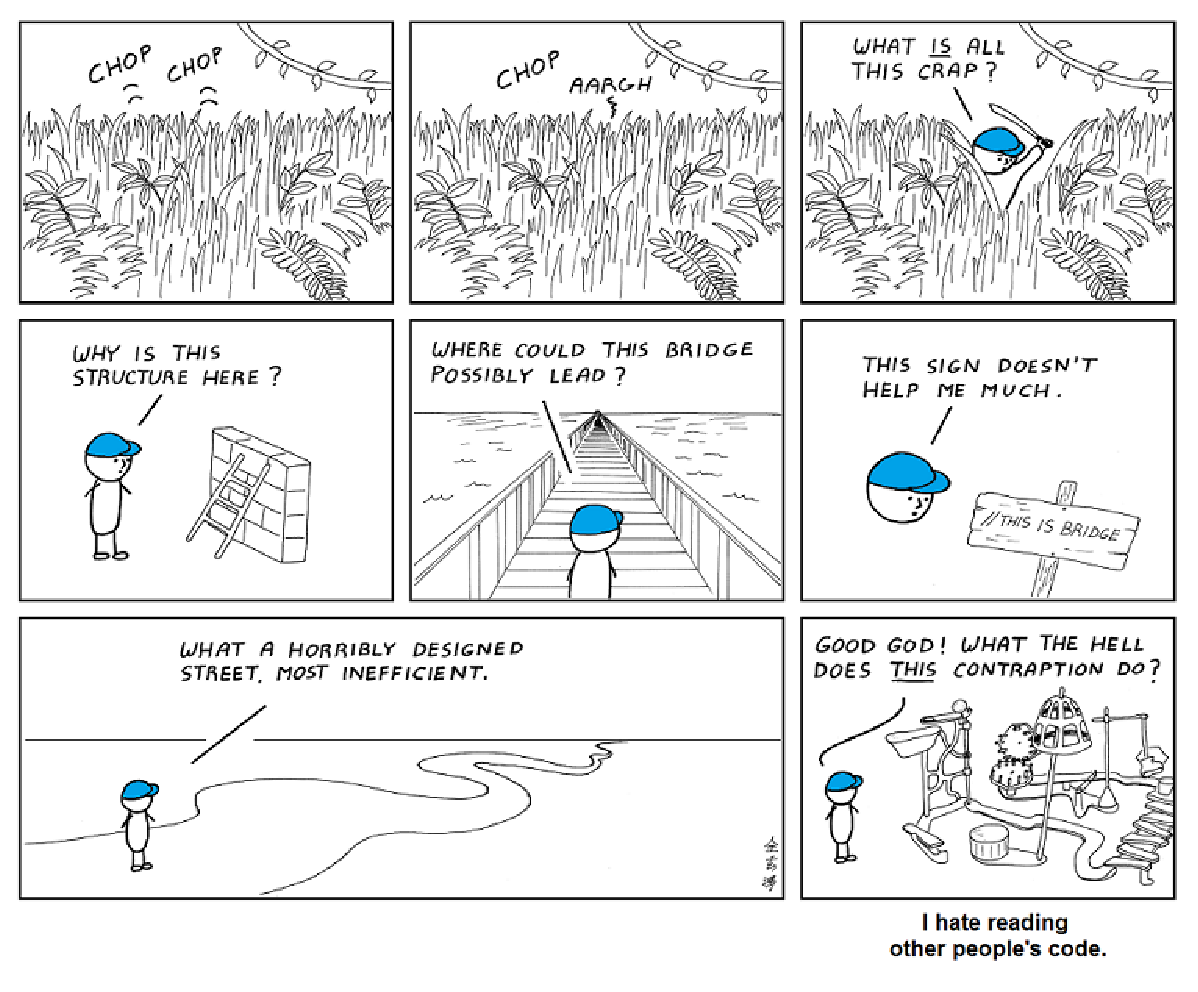
\includegraphics[scale=0.4]{comics/abstruse_goose_opc.eps}
\caption{Abstruse Goose \# ???: OPC}
\end{figure}

You could of course try to make this clear with
our variable names, say, by writing something like
\code{vector<int> stack}.
If you do this, it might convey your intention.
But of course, another interpretation would be that you had initially
written \code{Stack<int> stack}, and then later realized that you actually
needed extra functionality. But because you did not want to rename the
variable everywhere, you just changed its type to \code{vector<int>},
so even though the variable is called \code{stack}, it is not actually
used as one.

The upshot is that you should ideally declare your variables to be
of the type that you actually need, not giving yourself extra
functionality you do not intend to use. 
In particular, you may not find too many immediate uses for a
\code{Deque},
since most of the time, you will want either a \code{Stack} or \code{Queue}.


%%%%%%%%%%%%%%%%%%%%%%%%%%%%%%%%%%%%%%%%%%%%%%%%%%%%%%%%%%%%%%%%%%%
\chapter{Operator Overloading and Copy Constructors}
\label{chap:overloading}
[Note: this chapter covers material of about 1 lecture.]

%In this chapter, we will first learn about overloading and operators,
then see how to combine them to create easier-to-read code.
We will also see where and how copy constructors are used,
and learn about the difference between shallow and deep copying.

\section{Overloading and Operators}
Function overloading simply means having multiple functions of the
same name, but with different numbers or types of parameters.
For instance, when we write something like:
\begin{verbatim}
int minimum (int x, int y);
double minimum (double x, double y);
\end{verbatim}
we have overloaded the \code{minimum} function.
Doing this is perfectly acceptable:
when you write \code{cout << minimum (a, b)},
the compiler can tell from the arguments which of the two function to use.
It is only when you try to have two functions with the same exact
signature that you run into trouble:
\begin{verbatim}
bool foo (int x);
void foo (int y);
\end{verbatim}
Now, if you call \code{foo(a)} on an integer \code{a},
the compiler would not know which of the two functions you mean,
so it will not let you write this code in the first place. 
To summarize, \todef{overloading} is just having multiple functions of the same name.

\todef{Operators} are symbols such as 
\code{==}, \code{!=}, \code{=} (assignment), \code{<=}, \code{+},
\code{-}, \code{++}, \code{*} (multiplication, and dereferencing), \code{[]}, 
\code{<<}, \code{>>}, and many others.
Most operators are binary, that is, they take two arguments, such as
\code{x==y}, \code{x=y}, \code{a+b}, \code{a[i]}.
But there are also some unary ones (taking one argument),
such as \code{!b}, \code{*x}, \code{i++}.
For operators, C++ knows where the arguments go. For many operators
(\code{=}, \code{==}, \code{<=}, \code{+}, \code{<<}),
one argument goes before the operators, the other after.
But for instance, for \code{a[i]}, one argument goes ``in the middle''
of the operator.

Using operators is really just shorthand for calling a function.
When you write the following code:
\begin{verbatim}
    if ( a1 == a2 ) cout << "They are equal!";
\end{verbatim}
it actually gets translated to
\begin{verbatim}
    if (operator==(a1, a2)) operator<< (cout, "They are equal!");
\end{verbatim}
If you wanted, you could directly write the second version in your code.
The reason you should not do so is that it would be much harder to read.
In a sense, operator overloading is just what some people call
``syntactic sugar:'' parts of the programming language that do not
really add functionality,
or even necessarily good coding practices (like code reuse),
but just make your code look prettier. 
For instance, suppose that \code{x,y} are variables of some class you
have written yourself. Something like 
\begin{verbatim}
if (x > 0) y++;
   else if (x == 0) y = 0;
        else y --;
\end{verbatim}
is much easier to read than
\begin{verbatim}
if (isGreater(x,0)) addOne(y);
   else if (equals(x,0)) set(y,0);
        else subtractOne(y);
\end{verbatim}
or
\begin{verbatim}
if (x.isGreater(0)) y.addOne();
   else if (x.equals(0)) y.setEqual(0);
        else y.subtractOne();
\end{verbatim}

The ``long version'' of operator names
(such as \code{operator== (a1, a2)} in our earlier example)
does tell you how to overload operators in general:
all you need to do is to overload a function whose name is the word
\code{operator}, followed by the operator itself.
For instance, if you want to overload the \code{*} operator to allow
``multiplying'' a number by a string
(and define it to mean concatenating that many copies of the string),
you can do that as follows:
\begin{verbatim}
string operator* (int n, string x)
{
  string s;
  for (int i = 0; i < n; ++i) s.append (x);
  return s;
}
\end{verbatim}

You could now write something like
\code{cout << 5 * "Hello"} 
or \code{cout << operator* (5, "Hello")}.

\section{The \code{const} keyword}
The \code{const} keyword is not directly related to operator
overloading or copy constructors, but this is the context where it
makes a lot of sense and becomes important for the first time in this
class, so we have a discussion here.

When you initially learned about passing parameters to functions by
reference (with `\&`), the purpose was probably always so that the
function could modify the content of the variable,
and the modification would be seen by whichever other function had called it.
But there is another reason to pass parameters by reference: 
when you pass by value, a copy of your parameter is made,
which involves calling the copy constructor 
(see Section~\ref{sec:overloading:copy-constructors}).
There are some dangers to this:
if no copy constructor is implemented, the default is to make a shallow copy,
and in some cases, that is not what you want to happen. 
And if you do make a deep copy, that can be quite inefficient at times.
To avoid ambiguities like this,
when the types of your parameters are more complex
(like \code{vector} or our own \code{ArrayList}, or later on in
Chapter~\ref{chap:templates} generic/template types),
it is often easiest to just pass by reference.

But if you pass parameters by reference,
then someone using your function might suspect that you intend to
alter the object that is passed in, 
even when that is not your intention. 
The solution is to use the \code{const} keyword;
not only does it \emph{tell} the user of your class that the function
does not alter its argument,
but the compiler will \emph{ensure} that you cannot alter it. 
For instance, if you wanted to write a function \code{append} that
appends one \code{ArrayList} at the end of another,
its syntax would be as follows:

\begin{verbatim}
void ArrayList::append (const ArrayList & a2) {
    //code
}
\end{verbatim}
By adding \code{const}, you ensure that the code inside the function
can not alter the value of \code{a2} or any of its fields. 
If you tried to include code that alters \code{a2},
the compiler would return an error.%
\footnote{The exact meaning of ``altering'' \code{a2} is a bit subtle.
  To be precise, when you use the \code{const} keyword,
  you cannot make assignments to the member variables of \code{a2}.
  But if \code{a2} has a field that is a pointer
  (for instance, the internal array for the \code{ArrayList}),
  we \emph{are} allowed to change what is stored at the memory
  locations that the pointer points to.
  This may at first seem unintuitive.}
The main point of \code{const} is to make it clear to others using the
function(s) what can and cannot happen to the parameters.

Suppose that you are now implementing the \code{append} function,
and as part of your implementation,
you want to call some other member function on \code{a2}. 
How is the compiler supposed to know that this function call will not
suddenly result in changes to the member fields of \code{a2}?
This is where the second use of \code{const} comes in.
The syntax is like in the following example:

\begin{verbatim}
ArrayList::print () const {
    //code
}
\end{verbatim}
Say that we are defining a function to print the \code{ArrayList},
which should not need to alter any member fields of the object.
The \code{const} keyword now says that the function
\code{printlist} will not change the member variables of the object on
which it is called, that is, after it executes, the object will be in
the same state. 

There is a third use of the \code{const} keyword.
Sometimes, it is useful for a function to return its result by
reference.
This is typically for the same (or similar) reasons as those which
make you want to pass arguments by reference:
(1) you want to allow the code that calls the function to modify the
returned value, or
(2) the  returned value is a complex object, and you do not want a copy
constructor to be called for it.
In the second case, you again want to make it clear that the returned
object can/should not be altered.
You do this by returning a \code{const} reference.

All three uses are illustrated with the following example of the
\code{get} function of a \code{map} implementation:
% DK: the get function for maps has not really been defined here

\begin{verbatim}
const ValueType & Map::get(const KeyType & key) const;
\end{verbatim}

Because the key could be a complicated object,
you want to pass it in by reference, but the \code{get} function
should not modify it, so the key is passed in by \code{const} reference.
The \code{get} function should also not modify the state of the map,
so the whole function is declared \code{const}.
Finally, the value associated with the key could be a complex object,
so it is returned by reference;
but unless we want someone to be able to modify it
(and thus implicitly modify the map),
we should return it by \code{const} reference.
Notice that there are three objects around here:
the key, the value, and the map.
Each \code{const} refers to a different one among those three objects that
may not be altered.

Use the following as a guideline for when to mark things \code{const}
and when to pass by reference:
\begin{itemize}
\item If a member function does not need to alter the object on which
  it runs, then mark it \code{const}. It cannot hurt to do so,
  and might help you, because you can now call this function from within a
  context where the object is \code{const}.
\item If you are passing around complicated objects, unless you see a
  good reason to pass them by value, pass them by reference.
\item If you are passing an object by reference only for this reason,
  but not because the function you are writing is supposed to modify it,
  then pass it by \code{const} reference.
\item If you are returning an object by reference just because it is
  complicated, but not because you want to be able to alter it,
  then return it by \code{const} reference.
\end{itemize}

One more thing is worth mentioning about the \code{const} keyword,
because it often confuses students:
While the \code{const} keyword, applied to a member function,
prevents you from changing \emph{member} variables of the object
inside the function,
it of course does not prevent you from changing local variables of the
function, since they are not part of the object's state. 

\section{Operator Overloading and Classes}
By far the most frequent case for operator overloading is in the
context of defining new classes.
For instance, if you define your own class for complex numbers (as
we will do below), you would want to overload the arithmetic operations,
equality test, assignment, and a few others.
And for almost any class you define, you will likely want to overload
the assignment operator, the equality test \code{==}, and frequently
also \code{<<} so that you can easily print it to the screen or a file,
and do not have to write separate \code{print()} functions to
print to \code{cout, cerr} and files.

The syntax for operator overloading in classes is as follows.
Suppose that we have declared a class \code{IntArray},
which stores the size of the array and an array of integers internally.
We now want to add some operators:
\begin{verbatim}
class IntArray {
     // for binary operators
     // pattern: [RETURNTYPE] operator[OPERATOR] ([RHS DATA])
     // Example:
     bool operator== (const IntArray& otherArray) const {         
        if (this->size != otherArray.size) return false;
        else (for int i = 0; i < size; ++i)
             if (this->data[i] != otherArray.data[i]) return false;
        return true;
     }

     int & operator[] (int index) {
        return data[index];
     }

     // for unary operators
     // pattern: [RETURNTYPE] operator[OPERATOR]
     // Example:
     IntArray & operator++ () {
         // increment all entries in the data field.
         for (int i = 0; i < size; ++i) data[i] ++;
         return *this;
     }

     private:
       int size;
       int *data;
}
\end{verbatim}

We can now write things like
\begin{verbatim}
IntArray firstArray, secondArray;
// some computation to put data in the variables.
if (firstArray == secondArray) ++firstArray;
secondArray[0] = 0;
\end{verbatim}
as shorthand for
\begin{verbatim}
IntArray firstArray, secondArray;
// some computation to put data in the variables.
if (firstArray.operator==(secondArray)) firstArray.operator++;
secondArray.operator[](0) = 0;
\end{verbatim}

Two small notes: first, why do we have \code{++} return \code{*this}?
Could we have made the operator's return type void?
We could, but then we could not write things like \code{cout << ++a},
because the type of \code{++a} would be \code{void}.
Second, why did \code{operator[]} return its result by reference?
The reason is that we want to be able to overwrite it,
as we do in the example.
If we returned it by value, then overwriting would be impossible.

One type of operator we frequently overload is the assignment operator,
since we routinely want to write something like \code{x=y} for objects
of our own newly defined class.
A few interesting issues come up when you define assignment operators.
Let us try to write one for our \code{class IntArray} above:

\begin{verbatim}
IntArray & operator= (const IntArray & otherArray) {
    this->size = otherArray.size;
    this->data = new int[this->size];
    for (int i = 0; i < this->size; ++i)
        this->data[i] = otherArray.data[i];
    return *this;
}
\end{verbatim}

We just copied over all of the data from \code{otherArray}.
Why did we make the assignment operator's return type
\code{IntArray\&} instead of \code{void}?
The reason is the same as for the \code{++} operator earlier:
it allows us to write a statement such as \code{a = b = c},
which we routinely do with other types (like integers),
and would therefore like to do for \code{IntArray} as well.
For that reason, when we write \code{b=c},
what is returned must also be of the type that can be
assigned to \code{a}.

However, there is something else we should think about with the code
for the assignment operator.
Our class \code{IntArray} has dynamically allocated data
(here, an internal array), so when we write 
\code{this->data = new int[this->size]}, we create a memory leak.
We have to deallocate the old \code{data} object before making this
assignment.
So suppose that we added the statement \code{delete [] data}
as the first line of our operator. Are we good now?
Not quite. Think about what happens when we write the statement
\code{a = a}.
While this is not necessarily a very useful statement to write,
you would not want it to break someone else's code because
of \emph{your} wrong implementation of the operator. 
What happens now is that first, you delete all the data inside
\code{a}, then try to copy that (deleted) stuff into \code{a}.
So you will just copy garbage, and likely get a segfault
(if you are lucky) or really strange behavior.
So you must first check that you are not assigning an object to itself;
once you have ensured that, it is safe to deallocate the old data in
the object you are assigning to,
then copy over the data from the other object.
This means we should also add a first line
\code{if (this != \&otherArray)}.

\section{Friend Access}
Sticking with our integer array example, suppose that we wanted to
implement an operator that multiplies all entries of the array with
the same integer. We could do that as follows:
\begin{verbatim}
class IntArray { 
  // other stuff
  IntArray operator* const (int multiplier)
    { 
       IntArray newArray;
       newArray.size = size;
       newArray.data = new int[size];
       for (int i = 0; i < size; ++ i)
           newArray.data[i] = data[i] * multiplier;
       return newArray;
    }
}
\end{verbatim}
Now, we can write code like \code{a*7} to multiply the entire object
of type \code{IntArray} by 7. 
(Again, this is shorthand for \code{a.operator*(7)}.)
But what if we also wanted to write \code{7*a}?
That would be shorthand for \code{7.operator*(a)},
meaning that we would have to make our operator a member function of \code{int},
which we are not allowed to do.
So in this case, we will have to revert to the earlier method we saw
of defining the operator not as a member function of \code{IntArray}:

\begin{verbatim}
IntArray operator* (int multiplier, const IntArray & oldArray)
  { // same implementation }
\end{verbatim}

But now, we have another problem:
our implementation accessed private data fields,
and methods that are not member functions are not allowed to do that.
(For the purpose of this discussion, we ignore the fact that we could
instead use our assignment operator and the access to individual
elements using \code{[]}. We are trying to learn something new here.)
What can we do? We could just make the variables public,
but that would completely defeat the idea of hiding variables that
others do not need to see.
What we would really like to do is say that these variables are still
private, but we will make an exception just for this one particular
function \code{operator*}.
C++ has a mechanism for doing this:
you declare a function a \code{friend} of a class, as follows:

\begin{verbatim}
class IntArray {
   // other stuff
   friend IntArray operator* (int multiplier, const IntArray & oldArray);
}
\end{verbatim}

If we put this line in the definition of the class \code{IntArray},
we can then write the exact code as above outside the class,
and it does get access to private variables.
Notice that the \code{friend} declaration had to be inside the class
\code{IntArray}.
That makes sense: only the class itself should be allowed to provide
the privilege of accessing its private variables --- a function cannot
just get access to private variables by declaring itself a friend of
the class.


Multiplying an array by a number is nice, but it is not a
functionality that is often needed.
The most frequent use of \code{friend} functions is for implementing
the \code{<<} operator for output streams.
The way you do this is as follows:

\begin{verbatim}
class IntArray {
  // other stuff
  friend ostream & operator<< (ostream & o, const IntArray & a);
}

ostream & operator<< (ostream & o, const IntArray & a)
{ 
  for (int i = 0; i < a.size; ++ i)
      o << a.data[i] << " ";
  o << "\n";
  return o;
}
\end{verbatim}

Since we wanted to access private data fields of \code{a},
we declared \code{<<} a friend function of \code{IntArray}.
Also, by now you should have gotten used to the idea of why we return
an \code{ostream} here: it is so that we can write
\code{cout << a << "Hello World"}
with multiple \code{<<}.

\subsection{Friend Classes}
The following is not directly related to operator overloading,
but since we are talking about \code{friend} functions,
we should also talk about \code{friend} classes.
Sometimes, you want to allow not just one function,
but all functions of class X to access all private members of class A.
To do so, you can simply declare X a \code{friend} class of A. 
Just like with friend functions, the \code{friend} relationship must
of course be declared in class A, not in X. 
The code for declaring class X a friend of A is:

\begin{verbatim}
class A {
  public:
    friend class X;
  private:
    ...
}
\end{verbatim}

This piece of code would ensure that any object of type X would be
allowed to access all the private parts of any object of type A.

\section{An Illustration: Complex Numbers}
The following illustration shows in more detail how to actually code
with operator overloading 
(whereas the preceding discussion was perhaps a bit abstract). 

We want to implement a class for complex numbers.
Recall that complex numbers are of the form $a+\imath b$, where $a,b$ are
real numbers, and $\imath$ is such that $\imath^2 = -1$.
The addition of complex numbers is defined as expected:
$(a+\imath b) + (c+\imath d) = (a+c)+\imath (b+d)$.

We can use the following definition of a very basic \code{Complex}
class: 

\begin{verbatim}
class Complex {
  private:
    double re, im;	
  public:
    Complex (double re, double im) {
      this->re = re;
      this->im = im;
    }

    Complex (const Complex & toCopy) {
      // we add a copy constructor while we are at it.
      // See the next section to learn about copy constructors.
      this->re = toCopy->re;
      this->im = toCopy->im;
    }

    Complex add (Complex other) const {
      double reSum = re+other.re;
      double imSum = im+other.im;
      return Complex(reSum, imSum);
    }

    string toString() const {
      return (""+re+ "+" +im+"i");
    }
}
\end{verbatim}

Now, we could add two \code{Complex} numbers and print the sum using
the following code:
\begin{verbatim}
  Complex c1 = Complex(1.5,-3.2);
  Complex c2 = Complex(1.1,1.3);
  Complex sum = c1.add(c2);
  cout << sum.toString() << endl;
\end{verbatim}
	
While this works well, it is a little tedious to have to write
function calls like \code{add()} and \code{toString()}. 
This makes comprehending the code more difficult than it needs to be. 
To get around this, we can use the idea of operator overloading we
just saw.
Instead of (or in addition to) having a function \code{add()},
we overload the operator \code{+}, as follows:
\begin{verbatim}
  Complex operator+ (const Complex& other) const {
      return add(*this, other);
}
\end{verbatim}
		
Now, we can perform the third line of the code above using the
shortcut: 
\begin{verbatim}
   Complex sum = c1+c2;
\end{verbatim}

This is exactly equivalent to the previous segment,
but is much easier to interpret.
We overload a few more commonly used operators, to get a hang of it.

\begin{verbatim}
Complex operator- (const Complex & other) const {
   double reDiff = re - other.re;
   double imDiff = im - other.im;
   return Complex(reDiff, imDiff);
}

Complex operator* (const Complex & other) const {
   // look up multiplication of complex numbers if you do not remember it.
   double reProd = re*other.re - im*other.im;
   double imProd = re*other.im + im*other.re;
   return Complex(reProd, imProd);
}

bool operator==(const Complex & other) const {
   return (re==other.re && im== other.im);
}

bool operator!=(const Complex & other) const {
   return !(*this == other);
}

bool operator< (const Complex & other) const {
   double absSq = re*re+im*im;
   double otherAbsSq = other.re*other.re + other.im*other.im;
   return (absSq < otherAbsSq);
}

bool operator<= (const Complex & other) const {
   double absSq = re*re+im*im;
   double otherAbsSq = other.re*other.re + other.im*other.im;
   return (absSq <= otherAbsSq);
}

bool operator> (const Complex & other) const {
   return !(*this<=other);
}

bool operator>=(const Complex & other) const {
   return !(*this<other);
}
\end{verbatim}

With these definitions in place, we could now do arithmetic and
comparisons on our nice \code{Complex} class. 
In order to also be able to print them,
we will overload the operator \code{<<}.
Suppose that we did not already have the \code{toString()} function.
Then, to stream out the complex number,
we write the following simple function.

\begin{verbatim}
ostream & operator << (ostream &out, const Complex & c) {
    out << (c.re+ "+" +c.im+"i");
}
\end{verbatim}

Since we are accessing the private member variables,
we need to make this operator a \code{friend} function of the class
\code{Complex}, by putting the line

\begin{verbatim}
    friend otsream & operator<< (ostream &out, const Complex & c); 
\end{verbatim}

into the definition of \code{class Complex}.
We can now write code including multiple \code{<<} 
in one statement, as follows: 

\begin{verbatim}
  Complex c1 = Complex(1,2);
  Complex c2 = Complex(5,7);
  cout << c1 << " + " << c2 << " = " << c1+c2 << endl;
\end{verbatim}

\section{Copy Constructors}
\label{sec:overloading:copy-constructors}
When we started talking about classes and objects,
we also mentioned constructors briefly.
It is worth mentioning explicitly now that just like any other
functions, constructors can be overloaded; i.e.,
a single class can have many different constructors,
so long as their signatures (number/types of arguments) are different.

One type of constructor that is almost always very useful is a copy
constructor, which gets another object of the same type,
and ``copies'' its contents in some way.
Its signature will usually be:

\begin{verbatim}
class A {
   A (const A & otherA);
}
\end{verbatim}

With a copy constructor, we can ``copy'' objects as follows:

\begin{verbatim}
    A *a1;
    // some code to put stuff in a1.
    A *a2 = new A(a1);
    // a2 now contains a copy of a1.
\end{verbatim}

How much should a copy constructor copy?
That is quite an interesting question, and depends on context. 
One approach is to copy exactly the data fields of your object.
This is called a \todef{shallow copy} and is what C++ produces as a
default copy constructor if you do not write one yourself.
However, sometimes, that is not what you want.
For instance, in our example above of an integer array \code{IntArray},
a shallow constructor would copy the \code{size} and \code{data} variables.
Since \code{data} is a pointer, we would now have two objects whose
\code{data} pointers point to the same memory.
If we make an edit in one, it will edit the other.
Perhaps that is what we want, and perhaps not.
If it is not what we want, then what we wanted was likely to copy all
of the contents of the array to a new location as well.
In that case, we would be making a \todef{deep copy},
and we have to write a copy constructor to do it correctly.
Deep copies can involve a bit of work:
for instance, for a linked list, you would have to make a copy of
each element of the list, and link them all up correctly as you go along.
Often, that is exactly what you want from a copy.
So make sure you know exactly what you want to copy and why.
Otherwise, you may get surprising results.

To illustrate what can go wrong, suppose that for our \code{IntArray} above,
we make a shallow copy, with the following implementation:
\begin{verbatim}
class IntArray {
  // other stuff
  IntArray (const IntArray & otherArray)
    { size = otherArray.size; data = otherArray.data; }
  ~IntArray ()
    { delete [] data; data = NULL; }
}

int main (void)
{
  IntArray a1;
  IntArray a2 (a1);
  return 0;
}
\end{verbatim}

This program will segfault.
What happens is that \code{a2} will contain shallow copy of \code{a1}.
When the program terminates, the destructors of both objects are
called, to give them a chance to clean up their affairs before going
away (e.g., the objects may want to store some data on disk).
Suppose that \code{a1} gets destroyed first.
Then, its \code{data} gets deleted, and is deallocated. 
But the pointer \code{a2.data} still points to the location,
and when \code{a2} gets destroyed,
it tries to delete memory that has already been deallocated.
When you debug this program, you would wonder why it segfaults in the
line \code{return 0}, which seems rather innocuous.
This type of subtle errors can show up in unexpected parts of your
program, and is not infrequently caused by the wrong type of copy
constructor.  

Why are copy constructors so important?
To answer that question, let us return to our earlier discussion of
passing parameters by value vs.~passing them by reference.
You recall that in this class, we have been doing much of our passing
of parameters by reference,
and then declaring them \code{const} to avoid them getting altered.
So far, we have been a bit vague about ``passing around big objects,''
and ``it is not clear what happens when you pass a complicated object''
into a function as a parameter by value.
Actually, it \emph{is} clear what happens.
C++ generates code that initializes your local variable using a copy
constructor. So when you have the following code:
\begin{verbatim}
int foo (A myAObject)
  { ... }
\end{verbatim}
and you call \code{foo (b)}, what will happen is that \code{myAObject}
gets initialized via copy constructor from \code{b}.

Exactly the same thing applies when you have a function that returns
by value vs.~one that returns by reference.
When you return by value, the variable that you assign to
(or the place where the return value is used) gets initialized by copy 
constructor from what you return.

In both of the preceding cases, 
if the class \code{A} has a copy constructor that does exactly what
you want, passing complex objects by value is perfectly fine,
and your code should execute exactly as you expected
(except it may be a bit inefficient to copy so many objects). 
But if \code{A} makes a shallow copy when you needed a deep copy,
or makes a deep copy when you needed a shallow one,
then you could get very unexpected results.
In particular, because \code{myAObject} is a local variable,
it will be destroyed when \code{foo} ends.
If \code{myAObject} were a shallow copy of --- say --- an
\code{IntArray}, then the \code{data} of that \code{IntArray} would be
deallocated.
This would likely have terrible consequences elsewhere in the program.
And remember: when you have not explicitly defined a copy constructor,
C++ will generate a default one which performs a shallow copy.

This type of issue is even more pronounced when you write
templated/generic classes (as you will learn in Chapter~\ref{chap:templates}).
In that case, sticking with our previous example, you would not even
know what the class \code{A} is.
Some users may use your function \code{foo} with classes that have a
deep copy constructor,
others with classes that have a shallow copy constructor. 
Unless you are very sure that your function works equally well in both cases,
it is much safer to simply pass parameters by reference,
and side-step the use of a copy constructor altohgether.
And that is why we have been advocating passing complex parameters by reference.

\subsection{The Rule of Three}
Now that we have discussed in depth what a copy constructor does,
and when you should write one, we should ask:
what about the assignment operator?
Does it also need to be written?
The answer is typically that if you need to write your own copy
constructor (because you do not want the default shallow copy),
then you will virtually always also want your own assignment operator.
The reason is that when you need a deep copy from your copy constructor,
then a deep copy is probably the ``right'' way to copy objects of your
class. 
Then, an assignment such as \code{a = b} should probably also make a
deep copy, as it would be very surprising for a user that assignment
does not do the ``right'' thing.

And for that matter, if you need a deep copy, it is virtually always
because there is some dynamic memory allocated inside your object.
Then, you should also have a destructor which deallocates that memory.
The rule of thumb that we can derive is then the following (sometimes
called the ``Rule of Three''): If you implement one out of the
following three, then you almost always need to implement all three of
them:

\begin{itemize}
\item Copy constructor
\item Assignment operator
\item Destructor
\end{itemize}


% edited up to here


%%%%%%%%%%%%%%%%%%%%%%%%%%%%%%%%%%%%%%%%%%%%%%%%%%%%%%%%%%%%%%%%%%%
\chapter{Inheritance and Polymorphism}
\label{chap:inheritance}
[Note: this chapter covers material of about 1 lecture.]

%Suppose that a friend has coded an integer (or perhaps templated) \code{List}
class based on linked lists and you want to create a deluxe version of it. 
The deluxe class \code{DeluxeLinkedList} would do the same thing
except that it has an \code{isEmpty} function and an upgraded
version of your friend's \code{print} function.
There are two natural ways of accomplishing this. 
\begin{enumerate}
\item You could just change your friend's code everywhere. But your
  friend may not like this; perhaps, he/she needed the particular format
  of printing the list, and you just destroyed his/her code.
  In particular if you are working on a project together,
  both versions may be needed at the same time,
  so it is not just about choosing the ``better'' version.
\item You could just copy and paste your friend's code and write your own
  modifications into the copied version. But that also has problems:

\begin{itemize}
\item There are now two versions of the original code, so changes made
  to one have to be carefully copied over to the other.
  In particular, if your friend discovers a bug in his/her code,
  it now has to be fixed in two places (or more, if you made different versions).
\item Copying/pasting is very inelegant as a general programming
  technique.
\end{itemize}
\end{enumerate}

Both methods also require you to have access to your friend's complete source
code in the first place, and not just the compiled object files and headers.

The clean solution to this problem is called \todef{inheritance},
and it is one of the most central notions of object-oriented design/programming.
Given a class A, inheritance allows you to define a new class B that
``inherits'' (automatically copies) all data and functions from A. 
Further, it allows you to modify and add functions as necessary, and
overwrite existing functions. The basic syntax is as follows: 

\begin{verbatim}
class B : public A
{
  ...
}

\end{verbatim}
This code basically just copy-pastes everything from A into B
(except what you overwrite).
The difference is that as soon as something is changed in A,
the changed version is also used in B,
so you only need to fix things in one place, and
--- unless you use templates (which create some problems) ---
you do not even need access to the implementation of A, just the
header file and compiled version.

When you use inheritance, the class you are inheriting from (here, A) is
called the \todef{base class} or \todef{superclass}, while the class
that is doing the inheriting (here, B) is called the \todef{subclass}.

As far as our thinking is concerned, the code for A is copied into B.
Therefore, the same rules apply for overloading functions as are in
effect when you write your own class from scratch:
you may overload function names so long as the functions have
different signatures (numbers or types of arguments).
But, as we will see, you also get to \emph{replace} one function in A
with another function in B which has the same signature.

Now that you hopefully understand the basics of inheritance, 
let us build \code{DeluxeLinkedList} by inheriting from
\code{IntLinkedList}. 
First, we add a new function to test whether the list is empty:

\begin{verbatim}
bool DeluxeLinkedList::isEmpty () {
  return (this->head == nullptr);
}
\end{verbatim}

Then, we replace the \code{print} function (which had previously used
recursion to print the list in reverse order) with the following:

\begin{verbatim}
void DeluxeLinkedList::print() {
  for (Item *p = head; p != NULL; p = p->next)
     std::cout << p->value << " ";
  std::cout << std::endl;
}
\end{verbatim}

In addition, we put the two function headers inside 
\begin{verbatim}
class DeluxeLinkedList : public LinkedList
{
  public:
    void print ();
    bool isempty ();
}
\end{verbatim}

When we try to compile this, the compiler will note an error,
and claim that our \code{DeluxeLinkedList} does not have a variable
called \code{head}.
But we inherited from \code{LinkedList},
which does have a variable called \code{head}!

The problem is that \code{head} is declared as \code{private} in
\code{LinkedList}. The keyword \code{private} makes the variable
very restricted: not even an inheriting class gets to access the
variable (though of course the data item is stored in the class).
A version that resembles \code{private} but allows all inheriting
classes to access the variable directly is \code{protected}.
Here is a summary of who is and is not allowed to access variables or
functions of a class:

\begin{description}
\item[public:] everyone (other classes, this class) can access the field.
\item[private:] only objects of the same class can access the
  field. One object of class A may access the private fields of
  another object of class A.
\item[protected:] only objects of the same or inheriting classes can
  access the field.
\end{description}

When we replace the word \code{private} with \code{protected} in the
definition of \code{LinkedList}, everything works afterwards.

\section{Member Visibility, Multiple Inheritance, and calling Base Class Methods}

Inheritance raises a few interesting issues,
such as whether subclasses (the inheriting ones) can access methods
and variables from the superclasses,
how to inherit from multiple classes,
and how to explicitly call a member function of the base class when
you are also overwriting it in the inheriting class.
We will discuss those here.

\subsection{Inheritance and Visibility}
You were probably wondering why we were writing 
\code{class B : public A}; in particular, why we needed the word
\code{public} here.
When you have a class B inheriting from A, sometimes, you want to 
restrict access to variables that were \code{public} in A;
that is, you want to \emph{make} them \code{private} or
\code{protected} in B.
For instance, you may  want to inherit the functionality of a linked
list to use it, but show the world a different set of functions to
call, and keep the other ones only for internal use.
Then, you would want them to become private. 
To distinguish more precisely what should become private and what
should remain public, you can inherit in one of three ways:

\begin{description}
\item[public:] All elements in A have the same protection in B as
  they had in A, so everything stays as it was.
\item[protected:] Private elements of A remain private in B, but
  protected and public elements of A both become protected in B. In
  other words, the minimum protection level for elements of A is now
  \code{protected}.
\item[private:]	All elements of A become private in B.
\end{description}

So by writing \code{class B : private A} instead, we would ensure that
whatever B has inherited from A cannot be accessed from any other classes:
neither those inheriting from B, nor those using objects of type B.

Of course, it is important to remember that even when you inherit
privately, all variables and functions that were part of A are still
there in B --- they are just not accessible to the outside world.
But you may have some functions in B that use variables of A that are
now private
As a result, it is still possible to access those now-private
members indirectly, just not directly.

\subsection{Multiple inheritance}

C++ allows a single class to inherit from multiple classes.
We strongly advise you to not use this feature, as quite a few things
can go wrong. For instance, if the two classes you are inheriting from
have variables or functions of the same name, you get clashes.
For some discussion, look up ``C++ Diamond of Dread.''
If you find yourself inheriting from more than one class, it is often
a sign that you should rethink your program's class structure. 

The most frequent ``legitimate'' use of multiple inheritance is when
you want to genuinely inherit the functionality of one class, and add
functions to meet all the specs of a pure abstract class.
(We will talk about pure abstract classes momentarily.)
Then, from the second class, you really do not ``inherit'' per se,
but you just implement the functions that that class wants. 
Unfortunately, in C++, the only way to do that is multiple
inheritance. 

In other more naturally object-oriented languages (such as Java),
purely abstract classes which specify functions you would like to see
in your class are distinguished from actual classes;
in Java, they are called \todef{Interface}.
Then, you can say that your class \todef{inherits} one class,
and \todef{implements} another interface.
Unfortunately, C++ does not have a mechanism for this, so sometimes,
you are stuck with multiple inheritance.

\subsection{Calling Base Class Methods}
We overwrote the \code{print} function in our implementation of the
\code{DeluxeLinkedList} class. What happens if someone actually wanted
to call the \code{LinkedList} version of \code{print}?
For instance, suppose that instead of printing the elements in correct order,
we still wanted to stick with the reverse order of \code{LinkedList},
but we wanted to print a message before and after.
C++ allows you to do that, by explicitly putting the name of the class
in front of a call.
Generally, to call a function belonging to class A, you would write
\begin{verbatim}
  A::functionName(parameters);
\end{verbatim}

So specifically for the \code{print} function implementation, we would
write
\begin{verbatim}
DeluxeLinkedList::print () {
  std::cout << "This is the deluxe version of print\n";
  std::cout << "***********************************\n";
  LinkedList::print ();
  std::cout << "***********************************\n";
}
\end{verbatim}
Notice that the \code{print()} function does not recursively call
itself, as it calls the other version.
Of course, if we did not add a function of the same name
(as we did with \code{print} here),
we could leave out the \code{A::} part,
and just call it as \code{functionName(parameter)},
since the function is inherited, and part of our new class B.

\section{Class Relationships}
When you build a large project, you will often have objects of dozens,
or even hundreds, of different classes interacting in different ways.
While at first this may seem overwhelming, if you define your class
hierarchies and relationships carefully,
it actually helps you organize and understand the way your code works,
compared to just writing thousands of lines of code without much structure.
Forming high-level conceptual ideas about how your project is
organized can be really helpful.

The following three are very standard relationships between classes.%
\footnote{There is much more to learn along these lines:
  a topic called ``design patterns'' explores many different standard
  patterns in which classes interact.
  We will see several simple examples later in this class,
  including Iterators in Chapter~\ref{chap:iterators}.
  In the context of Qt and event-based programming, discussed in
  Chapter~\ref{chap:qt}, you also get interesting interaction patterns
  between classes.}

\begin{description}
\item[Is-A:] We say that B \todef{is a(n)} A if B is a more specific
version of A; B has all the functionality of A and then some more. 
For instance, every cat \emph{is a} mammal: it has all the abilities
of a generic mammal, plus many cat-specific ones.

When you write code, \emph{is a} relationships are typically
implemented by using public inheritance: you want all the
functionality of A to remain available,
while adding more functions or data to B.

\item[As-A:] B \todef{as a(n)} A refers to implementing a class B using
  the functionality of A. B will typically look like something
  completely different to the outside world, but internally, it is
  implemented by using just A's functionality.
For instance, when you sleep on someone's couch,
you are implementing the functionality of ``bed'' using a ``couch''.
(You implement ``bed'' \emph{as a} ``couch''
--- even though that is the opposite as you would refer
to it with the verb ``use''.)
If instead, you sit on the couch, you may be implementing the
functionality of ``chair'' using a ``couch''. 

When you write code, \emph{as a} relationships are typically
implemented by using protected or private inheritance:
you do not want other classes to see the underlying functionality;
instead, all you want to expose to whoever uses your class is the new
parts you are implementing.
In the examples above, that would be ``bed'' or ``chair;''
the fact that a ``couch'' was used internally should/will not be visible.

\item[Has-A] B \todef{has a(n)} A if one of the fields of B is of type A. 
For instance, your car probably \emph{has a} radio.
That does not mean that your car itself has a function ``switch station,''
but that it contains an object which itself has that function.

\emph{Has a} relationships require no inheritance;
they simply involve creating a member variable of type A in B. 
\end{description}

The boundaries between \emph{has a} and \emph{as a} can be pretty
fluid, and sometimes, it makes sense to think about solving a
particular design issue in either way. 
For instance, are we implementing a \code{Map} \emph{as a}
\code{List}, or does a Map \emph{contain} a List?
In implementing it, one can often use these two nearly
interchangably.
This distinction tends to give students a bit of trouble,
so make sure you understand it.

\section{Static vs.~Dynamic Binding}
We saw that when one class \code{B} inherits from another class \code{A},
it can overwrite/replace some of the functions that already existed in
\code{A}.
For instance, our \code{DeluxLinkedList} inherited from the more basic
\code{LinkedList},
and we changed the \code{print} function from one to the other.

One of the nice things that (public) inheritance does for us is that when
\code{B} inherits from \code{A},
then each object of type \code{B} has all the functionality of an
object of type \code{A}.
Therefore, we can assign objects of type \code{B} into variables of
type \code{A}.
In other words, for our example of \code{DeluxeLinkedList}
inheriting from \code{LinkedList},
the following would be valid code:

\begin{figure}[htb]
\begin{verbatim}
    LinkedList *p;
    DeluxeLinkedList *q = new DeluxeLinkedList ();
    p = q;
    p->print();
\end{verbatim}    
\caption{Which version of \code{print} is called? \label{code:InheritingLinkedList}}
\end{figure}

Because by our inheritance, every \code{DeluxeLinkedList} is-a
\code{LinkedList}, we can assign objects of type
\code{DeluxeLinkedList} into variables of type \code{LinkedList}.
And because objects of type \code{LinkedList} have a
\code{print} function, we can call it.

Notice that this assignment only works in this direction:
assigning a more specific object to a less specific variable.
This way, we can be sure that the actual object has all of the
required functionality.
It does not work the other way around.
Think about a real-world example:
we have one class ``human'' and one class ``student,''
which inherits from ``human.''
Every student has all the abilities of a generic human,
plus some extra ones.
When you need a human for a particular task (e.g., ``donate blood''),
you can just substitute a student if you want.
But when you need a student (e.g., for ``take exam''),
you cannot substitute just any human,
since they may not be of the right type to
know how to execute the necessary functions. 

What we just discussed works only for \todef[inheritance]{public} inheritance. 
If a class inherits from another privately or protectedly,
it does not have the same methods and variables visible,
so you may not be able to use it.
For instance, if you were planning to use your ``couch'' for sitting on it,
and you implemented ``bed'' as-a ``couch,'' then the bed is not
helpful:
by hiding the ``couch'' functionality,
it cannot be used as a couch any more.

Now that we know that we can use a \code{DeluxeLinkedList} anywhere
that a \code{LinkedList} has been called for,
the following question arises:
since \code{DeluxeLinkedList} and \code{LinkedList}  both
implement different versions of a \code{print} function,
which one is called in the last line?
We could try out two arguments:
\begin{enumerate}
\item The compiler knows that \code{p} points to an object of type
  \code{LinkedList}. It cannot really figure out by code
  analysis that it so happens that this time (not even always),
  \code{p} points to an object that is actually of type
  \code{DeluxeLinkedList}. 
  So the call must be to the version of \code{print} defined in \code{LinkedList}.
\item While the compiler does not know at compile time what exactly
  \code{p} points to, when it comes time to actually \emph{call} a
  function (during execution), it must know the precise object that is
  pointed to by \code{p},
  and it so happens to be of type \code{DeluxeLinkedList}. 
  Therefore, the call will be to the version of \code{print} defined in
  \code{DeluxeLinkedList}.
\end{enumerate}

It turns out that both are by themselves valid arguments.
The first version is the default.
If you do not put any additional instructions in the code,
C++ will call the version of the function corresponding
to the declared type of the variable you are using.
This is called \todef{static binding}.

But sometimes, you would really like the second option to happen
--- you will see some examples in a moment.
You can tell the compiler to do this,
by declaring the \code{print} function to be \todef[function]{virtual}.
You do this by just adding the word \code{virtual} in the definition of
the function (both in the parent and child class), as follows:
\begin{verbatim}
class LinkedList {
   ...
   virtual void print ();
   ...
}
\end{verbatim}

The keyword \code{virtual} tells the compiler to not try to figure out
at compile time which version of the function to call,
but leave that decision until runtime,
when it knows precisely the type of the object.
This process --- figuring out which version of the function to
call at runtime --- is called \todef{dynamic binding},
as opposed to \todef{static binding},
which is when the compiler figures out at
compile time which version to call.

\section{Pure virtual functions and abstract classes}
Sometimes, you want to declare a function in a class, but not implement
it at all; you will see in a moment why.
Such a function is called a \todef{pure virtual function}.
The declaration lives entirely in the base classes' header files,
and you do not need to care about it at all in the implementation files.
The syntax is 

\begin{verbatim}
class A {
  public:
  virtual void print() = 0;
}
\end{verbatim}

The \code{= 0} part tells the compiler that the class does not
implement this function.
Of course, if a class has one or more pure virtual functions in it,
the class cannot be instantiated.
Such a class is called an \todef{abstract class}.
No object can be created from an abstract class.
After all, if we could create objects,
then what would code like the following do?

\begin{verbatim}
A obj;
obj.print();
\end{verbatim}
What code should be executed when the execution gets to \code{obj->print()}?
There is no function to call.
But if you can never instantiate an abstract class,
why would there ever be any reason to even define one?

\subsection{Why and how to use pure virtual functions}
The main reason to create pure virtual functions is to force
inheriting classes to implement a function.
For instance, in the example above, if we later implement classes
\code{B} and \code{C} which inherit from \code{A},
we have forced both of them to provide a \code{print()} function.
So we can safely call the \code{print()} function on them.

Pure virtual functions and abstract classes are very useful in
structuring one's classes,
and in avoiding code (and error) duplication.
For a standard example, imagine that you are developing a graphics
program that lets you draw basic shapes.
Since all graphics objects (rectangles, circles, polygons, etc.)
share some properties (such as perhaps color, line width, line style,
and a few others)
and maybe also some functionality,
you may want to define a general class
\code{GraphicsObject} which captures those.
You also want each of these objects to provide some functions, such as
perhaps \code{draw} (drawing itself), \code{resize}, or others.
But absent a specific definition of an object type (e.g., circle), you
cannot implement these functions yet.
Yet, you want to force all \code{GraphicsObject} objects you later
define to provide these functions,
so that you can put them all in one big array and process them the
same way.
In other words, you would like to do something like the following:
\begin{verbatim}
  List<GraphicsObject> allMyObjects;
  // code that loads a bunch of different objects into the list.
  for (int i = 0; i < allMyObject.size(); i ++)
     allMyObjects[i].draw();
\end{verbatim}
Even though \code{allMyObjects} may contain many different types of
graphics objects, so long as all of them inherit from
\code{GraphicsObject}, and thus have to implement a \code{draw()}
function, the code shown above will work perfectly fine.

The way to achieve this is to declare pure virtual functions
\code{draw()}, \code{resize()}, and whatever other functions you want.
Now, all classes you define later (like \code{Circle},
\code{Rectangle}, \code{Polygon}, etc.) that inherit from 
\code{GraphicsObject} must implement this function in order to have
objects generated from them.

Abstract classes are also very useful to specify an abstract data
type, and separate its functionality from its implementation.
After all, we have said before that an abstract data type is
characterized by the functions it supports, and there may be many ways
to implement them.
For example, a while back, we specified the ADT \code{Set},
which looks as follows when written as an abstract class.
(Say we are interested in sets of integers.)

\begin{verbatim}
class Set {
  public :
     virtual void add (int item) = 0;
     virtual void remove (int item) = 0;
     virtual bool contains (int item) const = 0;
}
\end{verbatim}

The preceding piece of code only says that any class that wants to
implement a \code{Set} must provide these functions.
Another programmer can then create, say, a \code{LinkedListSet}, an
\code{ArraySet}, a \code{VectorSet}, etc.
All of these classes would inherit from \code{Set} and implement the
functions, though they could do so in very different ways.
By inheriting from the abstract class \code{Set}, these other classes
have made sure to be very easily interchanged, as follows:

\begin{verbatim}
   Set * p;
   p = new LinkedListSet();
   ... // some time later
   delete p;
   p = new ArraySet();
\end{verbatim}
Using dynamic binding here (indicated by the \code{virtual} keyword),
the code has no problem calling the right version of each function,
and we can use different implementations interchangeably.

What would happen if we tried to define something
like a non-virtual unimplemented function?
\begin{verbatim}
  void add (int n) = 0;
\end{verbatim}
This results in an error. There is no point in having a non-virtual
non-defined function. If it is not defined, it cannot be called.
And if it is not virtual, then when it is overwritten later, the compiler
cannot figure out to call the overwriting version, unless the object is
already of type \code{B}, in which case there is no need for inheriting.

\medskip

Another classic reason for using pure virtual functions is that we can 
often avoid rewriting very similar code.
For instance, imagine that we are implementing an abstract data type
(say, \code{List}),
and focus on variants of the \code{insert} function. 
In addition to the basic \code{insert} version, you want to provide
several special functions, like \code{pushback} (which inserts at the
end), \code{pushfront} (which inserts at the beginning), and maye also
others.

Since the additional functions like \code{pushback} can be described
in terms of \code{insert}, you could write code like the following: 

\begin{verbatim}
class IncompleteList {
    public:
       void pushback (int item);
       void pushfront (int item);
       void insert (int n, int item) = 0;
}
\end{verbatim}

You could then implement the \code{pushback} and \code{pushfront}
functions once and for all, and reuse the code in this way. 
Something like the following:

\begin{verbatim}
IncompleteList::pushback (int item) {
  insert (size(), item);
}

IncompleteList::pushfront (int item) {
  insert (0, item);
}
\end{verbatim}
Then, our \code{LinkedList} and \code{ArrayList} and
\code{VectorList} would not have to implement each of the functions
\code{pushback}, \code{pushfront}, from scratch, but would just
need to provide the missing piece \code{insert}.
Because the \code{insert} function is virtual,
whenever in the course of executing \code{pushfront},
the program runs into \code{insert},
it determines at runtime which version of \code{insert} to call. 

This concept --- determining which version of a class member function
to call at runtime --- is called \todef{polymorphism}, which literally
means ``many forms:'' the object stored in a variable could be of one of
many forms, and the execution will do ``the right thing'' for the
current object.

\section{Constructors and Destructors with Inheritance}

Suppose that you have a class B which is inheriting from A. What
happens when you write something like the following piece of code?

\begin{verbatim}
B *myB = new B ();
\end{verbatim}

First, appropriate space is reserved on the heap for the object of
type B. But then, a constructor needs to be called. You will clearly
want to call a constructor for B; in the given code, it will be the
default constructor.
But if A has some private variables (which B inherits),
how will they get initialized?
The answer is that \emph{before} the constructor of the class B is
called, C++ calls a constructor for the class A.
If you do not explicitly specify which constructor for A to call,
C++ will substitute the default constructor.
If you want to call another constructor, you have to say so explicitly.

Here is how you do this.
Suppose that A has a constructor that passes a \code{string} as a parameter.
For B, you want to implement a constructor that gets a \code{string}
and an \code{int}, and uses A's constructor with a string.
You would write code like the following:

\begin{verbatim}
class B : public A {
  public:
    B (string s, int n) : A (s)
     { rest of the code here }
}
\end{verbatim}

% edited up to here

After the name of the constructor, you put a colon and then the
constructor you want to call from the superclass.
Again: it is important to remember that C++ always calls constructors
for all superclasses before the constructor for the class itself.

How about destructors? The same argument suggests that in addition to
the destructor for B, we will also need to call the destructor for A
at some point. After all, A may have dynamically allocated memory for
a private variable, and the only way to safely deallocate it is to
have A's destructor take care of it.

Calls to destructors happen in the reverse order of constructors. That
is, first the destructor of B is called, and then the destructor of
A. This makes sense, since B's stuff is built ``on top of'' A: so we
need to cleanly remove B's stuff first before it is safe to remove the
stuff from A.

For destructors, since classes only have one (with no parameters), you
don't have to worry about explicitly calling one or the other. C++
takes care of the destructor call chain for you; all you need to do is
be aware of it, and not destroy in the destructor of B any data that
you will then again attempt to destroy in A. 

However, something that you should \emph{always} do whenever you have
classes that are inheriting or being inherited from is making the
destructors \code{virtual}. This is very important for the following
reason. Look back at our example in
Figure~\ref{code:InheritingLinkedList}. When we call
\code{delete p}, which destructor is supposed to be called?
Clearly, since we have an object of type \code{DeluxeLinkedList}, it
may have extra data, so it would be important to call its
destructor. But if the destructor is not virtual, then C++ can only go
by the ``official'' type of \code{p}, which is \code{LinkedList}. It
would call the wrong destructor, which may result in a memory leak or
worse. For that reason, any class that has any chance of being
inherited from, and any class that inherits from another, should make
the destructor virtual.

As a general rule for both constructors and destructors, the
constructor and destructor of inheriting classes should take care of
the additional issues for their own class, but leave the other parts
to the superclass.

Also notice that if you have an abstract class, you do not need to
implement any constructors or destructors for it --- in particular,
for a pure abstract class, it makes no sense to build constructors or
destructors.


%%%%%%%%%%%%%%%%%%%%%%%%%%%%%%%%%%%%%%%%%%%%%%%%%%%%%%%%%%%%%%%%%%%
\chapter{C++ Standard Template Library}
\label{chap:STL}
[Note: this chapter covers material of about 0.5 lectures.]

%The ADTs we have learned about and implemented so far, and
most of the ones we will learn about later, actually come
pre-implemented with C++, in the Standard Template Library (STL).
The STL also contains implementations of several frequently used
algorithms. 

While many students surely have been waiting eagerly to use STL
implementations instead of having to code data types from scratch,
some may wonder why one would use STL. The advantage of standard
libraries is that they save us some coding, and more importantly, a
lot of debugging, as they presumably have been much more carefully
debugged than our own code. When our own project is big enough, we'd
like to avoid having to debug the basic data structures \emph{in
  addition to} the high-level logic.
The contents of STL can be roughly categorized as follows:

\begin{description}
\item[Containers]: These are data structures; the name arises because
  they \emph{contain} items. They can be further divided as follows:
\begin{enumerate}
\item Sequence containers: These are data structures in which items
  are accessed by the position they are stored at, like arrays.
  Our example from class was called \code{List}.
\item Associative containers: Here, items are accessed via their
  ``identity'' or key. The user does not know which index an element
  is stored at --- in fact, there may not be a clear notion of an index.
  The associative data structures we have seen are \code{Set} and
  \code{Map}.
\item Adapters: these are restricted interfaces that give you specific
  functionality, such as \code{Stack}, \code{Queue}, or \code{Priority
    Queue} (we'll learn about that one soon). 
  They are often implemented on top of other classes, such 
    as \code{List}.
\end{enumerate}
		
\item[Algorithms]: To use pre-implemented algorithms, you should
\code{\#include<algorithm>}. The algorithms all live in the 
\code{namespace std}. They are roughly divided as follows:
\begin{enumerate}
\item Search and compare: these are mostly iterator-based. They allow
  you to run some algorithm (compare elements to a given one, count/add all
  elements, etc.) on all elements of a container.
  To use these algorithms, you need to pass in an iterator of the
  container. A brief introduction to iterators is given below, and we
  will discuss them in more detail later in the semester, and in
  Chapter~\ref{chap:iterators}. 
%  Referring back to the discussion of the Map-Reduce paradigm we
%  talked about in the context of iterators, these are typical
%  functions that would contribute the ``Reduce'' side.
\item Sequence modification: These will affect the entire container,
  such as filling an array with zeros, or performing a computation on
  all elements. They are also iterator-based. 
%  In the context of the Map-Reduce paradigm, these algorithms would
%  fit with the ``Map'' part.
\item Miscellaneous: These contain mostly sorting algorithms, and
  algorithms for manipulating heaps, but also computing moments of a
  distribution and partitioning items. 
\end{enumerate}
\end{description}

\section{More Details on Container Classes}

All containers implement at least the following functions:
\begin{verbatim}
bool empty();
unsigned int size();
operator= is overloaded
iterators
\end{verbatim}
	
The \code{size()} function doesn't tell you how many elements are in
the container, but rather how many elements it can hold (which we
typically call its \emph{capacity} in class). 
	
For all of the container classes described next, if you want to use
them, you need to \code{\#include<container-name>}, where
\code{container-name} is the name of the container you wish to use.
You also must either use \code{namespace std} or precede each
container name with \code{std::}. Remember that except in your main
file, using \code{namespace std} is generally a bad idea, as it forces
every program that includes your code to use that namespace, sometimes
causing clashes in variable or class names.
	
Also, as the name says, these classes are ``templated.'' 
This means that you can easily build stacks, queueues, maps, etc., with
any kinds of data stored in them (whereas earlier, we just built them
for integers). You will learn later, in Chapter~\ref{chap:templates},
how to build your own template classes. (It's not difficult, but can
cause compiler/linker errors if you're not careful.) For now, you need
to know how to use them. That's actually not hard. 
When STL has declarations such as

\begin{verbatim}
template <class T>
class stack { 
  ...
  void push (T item);
  ...
};

template <class keyType, class valueType>
class map { 
  ...
  void erase (keyType key);
  ...
}
\end{verbatim}

you can define your own versions as follows:
\begin{verbatim}
stack<string> myStringStack;
map<int,bool> myIntToBoolMap;
\end{verbatim}

You can substitute any types there, including ones you have defined
yourself, or other container types. (For instance, you could have a
map each of whose values is a stack.) To use the functions, you can
now write

\begin{verbatim}
string s = "Hello World";

myStringStack.push (s);
myIntToBoolMap.erase (5);
\end{verbatim}

In other words, C++ will automatically make sure that the right
functions exist for the types you specified.

\subsection{Sequence Containers}
As we mentioned above, sequence containers are
similar to \code{List<T>} from class, in that they implement access to
elements typically by index position.
They allow reading, overwriting, inserting, and removing. 
Also, most of them implement swapping, and several other functions.
There are several sequence container classes, with different tradeoffs
and implementations.

\begin{description}
\item[\code{vector<T>}]: This is basically our \code{List<T>} type,
implemented using an expanding (doubling) array internally.

\item[\code{array<T>}]: This implements a fixed-size array,
i.e., it does not grow and does not provide \code{insert} or \code{remove}. 
Its interface and functionality is basically the same as a standard array.
(It is available only starting with C++11.)

The main advantage over \code{T* a = new T[100]} is that it catches
array indices out of bounds and throws exceptions, instead of leading
to segfaults or other bad errors.
			
\item[\code{list<T>}]: This is a doubly-linked list. It does not allow
access by index. 
In C++11, there is also a singly linked list as \code{forwardlist<T>};
it saves a bit of memory.
The linked list contains some additional list-specific operations such
as combining and splicing lists.
			
\item[\code{deque<T>}]: This is \emph{not} a \code{deque} in the
sense that it combines a \code{stack} with a \code{queue}.
Rather, it is a data type similar to \code{vector<T>}, but implemented
with non-contiguous memory blocks. (Basically, it internally keeps a
lookup table which of multiple separate memory blocks to access when a
particular index is requested.)

Because it does not need to copy over all elements when the size
grows, inserting elements is faster.
On the other hand, some operations have more complex implementations
and are a bit slower. 
If you anticipate that you will be spending a lot of time growing your
arrays, consider using \code{deque<T>} instead of \code{vector<T>}.
\end{description}
		
\subsection{Adapter Containers}
The adapter containers are called this because they ``adapt'' the
interface of another class, and are not implemented from scratch.
They provide special and restricted functionality.
The three adapters in STL are \code{stack<T>}, \code{queue<T>}, and 
\code{priority-queue<T>}, implementing the data types we have learned
about in this class, or (in the case of \code{priority-queue<T>}) will
learn about soon.

\subsection{Associative Containers}
In sequence containers, we access elements by their position in the
container, so it matters \emph{where exactly} an element is stored.
In associative containers, we only know that we want to insert,
remove, and look up elements, but we don't care where or how they are
stored, so long as the data structure can find them for us (by their
identity or key) when we want to access them.

The two associative container types we have seen so far are
\code{Set<T>} and \code{Map<T1, T2>}. Recall that \code{Set<T>}
provides the following functions:
	
\begin{verbatim}
   insert(T item)
   remove(T item)
   bool contains(T item)
\end{verbatim}
			
A \emph{Map/Dictionary} is similar, but it creates an association between
a key (such as a word) and a value (such as the definition of the word).
The name used in STL and elsewhere is usually \code{map}.
The functions that a map should provide are:
			
\begin{verbatim}
   insert (keyType & key, valueType & value)
   remove (keyType & key)
   valueType & lookUp (keyType & key)
\end{verbatim}
			
While this is how we have been thinking about sets and maps, the
actual implementation and naming in STL is a little different, as
described below.

\subsubsection{Different Set/Map classes}
STL provides implementations of \code{set} and \code{map}, differing
in several parameters.
\begin{description}				
\item[\code{set<T>}]: implements a set that can contain at most one
  copy of each element, i.e., no two elements may have the same key.
\item[\code{multiset<T>}]: implements a multiset of elements, which
  means that it may contain multiple elements with the same key.
\item[\code{map<keyType, valueType>}]: implements a map from keys to values, ensuring
  that there is at most one copy of each key.
\item[\code{multimap<keyType, valueType}]: implements a map from keys to values that
  allows the data structure to contain more than one copy of a key.
\end{description}

All of these data types are implemented using balanced search trees
(which we will learn about in a month or so). 
What this means is that you will have to provide a comparison operator
(i.e., overload \code{<=}, \code{<} etc.)
for your type \code{T} if you want to use these types, or hope that
whatever default is implemented will work well enough.

There is an alternative implementation using hash tables (which we
will learn about right after balanced trees). 
To access those implementations instead, you put the word 
\code{unordered\_} in front of the type's name, e.g.,
\code{unordered\_{}map}.

The hash table implementation is often faster, but it depends on a
good implementation of a hash function, which you may have to write
and provide yourself to suit your type \code{T}.
On the other hand, the tree-based version is very fast at iterating
over all entries in sorted order, since that's how they are stored
internally anyway.

\subsubsection{Functions in STL Set/Map classes}
Here are the most relevant functions for set in STL:

\begin{description}
\item[\code{set::insert (T element)}]: inserts the element into the set. It
  returns an iterator to the element, but this is usually not so
  relevant for you.
\item[\code{void set::erase (T element)}]: removes the element from the set.
\item[\code{size\_type set::count (T element)}]: returns the number of times
  the element occurs in the set, which is 0 or 1 for a regular set
  (not multiset). Allows you to test if the set contains the element.
\item[\code{iterator set::find (T element)}]: returns an iterator to the
  element in the set. You can use this for removing the element. If
  the element is not in the set \code{s}, the iterator will be equal
  to \code{s.end()}; see the discussion of iterators below.
\end{description}

For maps, while we had written \code{add} as a function with two parameters,
the way it is actually implemented in STL is with just a single
parameter, which is of type \code{pair}; a \code{pair} is just a
\code{struct} of two individual types. It is essentially defined as follows:

\begin{verbatim}
template <class S, class T>
class pair {
  public:
  S first;
  T second;

  Pair (S s, T t) { first = s; second = t; }
}
\end{verbatim}

This type is used in a number of places, as we will see. Throughout
the following list, we assume that we have a \code{map<keyType, valueType>}.

\begin{description}
\item[\code{map::insert (pair<keyType,valueType>)}]: inserts the association
  between \code{p.first} and \code{p.second} into the map, and returns
  an iterator to that element. If the map already contained an
  association for the key \code{p.first}, \code{insert} does not
  change anything, and instead returns an iterator to the existing pair.
\item[\code{void map::erase (keyType key)}]: removes the association for
  \code{key} from the map. If there was no association for the key, it
  doesn't do anything.
\item[\code{size\_type map::count (keyType key)}]: returns the number of
  associations for the given \code{key}, which is 0 or 1 for a regular
  map (not multimap). Allows you to test if the map already has an
  assignment for the key.
\item[\code{iterator map::find (keyType key)}]: returns an iterator to the
  pair \code{(key, value)} associated with \code{key} in the map. 
  If the key has no association in the map \code{m}, the iterator will
  be equal to \code{m.end()}; see the discussion of iterators below.
  The iterator iterates over \emph{pairs}, so if you want to extract
  the value, you get it with \code{m.find(key)->second} (and the
  key itself should be \code{m.find(key)->first}). Make sure to test
  that there was actually a mapping for your \code{key} before you
  dereference the iterator.
\item[\code{valueType \& map::operator[] (keyType key)}]: allows you to
  treat your map essentially like an array, by writing things like
\begin{verbatim}
map<string, int> myMap;
myMap["Hello World"] = 101;
myMap["Hello World"] = 103;
myMap["Thanks for the fish!"] = 42;
cout << myMap["Hello World"];
\end{verbatim}
  Different from the \code{insert} function, this one allows you to
  overwrite the mapping for a given key, e.g., the code above would
  output \code{103}. When you try to read the value for a key that
  isn't in the map, this will \emph{insert} the key into the map, with
  some dummy value assigned to it. It will then return the dummy
  value. So be forewarned in using this!
\end{description}

\subsection{Iterators}
Iterators are a systematic and unified way of traversing arrays and
other data structures. You will learn much more about them (including
how to write your own) in Chapter~\ref{chap:iterators}. For now, just
a quick primer on how to use them.

When you go through an array with a loop, your code might look like
the following:

\begin{verbatim}
int a[10];
int *i;

for (i = a; i < a + 10; ++ i) 
   cout << (*i);
\end{verbatim}

Notice that instead of writing \code{a[i]}, we basically treated the
index itself as a pointer. Iterators try to resemble this code as much
as possible. When you have a data structure that implements/allows
iterators, it will give you two functions: \code{a.begin()} and
\code{a.end()}. The former gives you an iterator pointing to the
``first'' element, and the latter an iterator pointing to the element
just after you are done (which in the above loop is \code{a+10}). So
you would write code like this:

\begin{verbatim}
MyDataStructure a;
iterator i;

for (i = a.begin(); i != a.end(); ++ i)
   cout << (*i);
\end{verbatim}

Iterators typically overload \code{=}, \code{==}, \code{!=},
\code{++}, \code{*}, and \code{->} so that your code looks as similar
as possible to the loop over arrays. It is convention that
\code{a.end()} is used for ``We're done''.

Therefore, when \code{it = map::find(...)} returns an iterator, its value will
equal \code{m.end()} if the element was not found, and otherwise, it
can be treated almost like a pointer in an array. In particular, you
can use \code{*it} to get to the \emph{pair} that the iterators is
pointing to, and \code{(*it).second} or \code{it->second} to reference
its second component, which is the value you want.

You can also output all the values in a map with an iterator, as
follows:
\begin{verbatim}
map<string, int> m;
// put stuff into the map here first

for (iterator it = m.begin(); it != m.end(); ++it)
   cout << "Key: " << it->first << "  Value: " << it->second << "\n";
\end{verbatim}




%%%%%%%%%%%%%%%%%%%%%%%%%%%%%%%%%%%%%%%%%%%%%%%%%%%%%%%%%%%%%%%%%%%
\chapter{Error Handling and Exceptions}
\label{chap:exceptions}
[Note: this chapter covers material of about 0.5 lectures.]

%\section{Handling errors}
In previous lectures, we implemented a linked list.
Suppose that we had added a function 
\code{int get (int position)} which returns the element at the given
position. 
Now someone else who got hold of our code writes the following:

\begin{verbatim}
    LinkedList *LL = new LinkedList;
    for (int i = 0; i < 10; i ++) LL->append (i);
    cout << s->get(15) << endl;
\end{verbatim}

When \texttt{get(15)} is called, the List does not have 15 elements
yet. What should be returned?
If we ran a loop of 15 steps through the list, the result here will
likely be an attempt at dereferencing a \code{NULL} pointer,
triggering a segfault.
The program will quit, and the person using our Linked List will not
really know what went wrong (except after some debugging). 
Also, simply ending the program may not be the right thing to do here.
What's the right way to deal with this problem?

\begin{itemize}
\item The simplest way is to claim that this is not your problem, and hold
the user responsible for correct usage of your code.
This falls into the broader paradigm ``garbage in, garbage out''. 
This is not a completely unreasonable position to hold; 
the person wanting to use your class should make sure to test whether
the stack is empty before accessing it.
But as we all know, ``should'' does not mean ``will'', and your goal
when writing code is not necessarily to help others develop good
habits, but to develop good code yourself.

\item A second idea would be to return a `magic' value like -1.
This might work when the list is known to only contain positive
values; the programmer could then use the unexpected return to debug
their code. 
However, if the list can contain any integers, there is no ``safe''
magic value. And for a more general list (of a templated type), this
solution is untenable, as we wouldn't even know what to return. 
Further, the programmer might simply choose to ignore bad
returns, which would cause errors to trickle up.

\item A third, and somewhat better, approach is to use the \code{assert}
statement.
In general, \code{assert} statements are good debugging technique.
For instance, we could insert the statement
\code{assert (position < this->size())} as a first line of
\code{get()}. 
(To use \code{assert} statements, you need to \code{\#include<cassert>}.)

An \code{assert} statement simply causes the program to crash when the
asserted condition fails to hold. While this is still a crash, at
least, it gives more useful information, namely, printing in which
line the crash happened, and what condition failed. This helps
significantly in debugging.
However, the program still crashes, which means that it does not have
the option of dealing with the error themselves.
\end{itemize}

These solutions all still involve crashes, which may not be the best
way to handle mistakes, e.g., if you're running the backend database
for a major website, or the control software for a rocket or a nuclear
power plant.
Instead, it would be better to actually signal to the caller of our
function that something went wrong (and what), and give it a chance to
handle the mistake.

\section{Setting Flags}
The way errors are traditionally signaled in C is by making the
function return a \code{bool} instead of the actual value we're
interested in, and passing the actual value by reference in another
variable. The following example illustrates this:

\begin{verbatim}
bool LinkedList::get (int position, int & val) 
{
   if (position < this->size()) {
      Item *p = head;
      for (int i = 0; i < position; i ++)
        p = p->next;
      val = p->value;
      return true;
    } else return false;
}
\end{verbatim}

This is a significant improvement. A slight downside is that the
calling function may still ignore the \code{bool} value, and simply
use the undefined value in \code{val}. 

\section{Exceptions}
The C++ solution is to use exceptions. 
Exceptions allow us to provide feedback about the success of an
operation, in such a way that a caller \emph{must} deal with the
failure condition explicitly.
The basic use of an exception is as follows: 

\begin{enumerate}
\item Upon failure, the method notifies the calling code by
  ``throwing'' an exception.
\item This exception propagates ``up'' through the program stack until
  it reaches a piece of code designed to handle it; it continues
  there. 
\item If no such code is found, the program terminates. 
\end{enumerate}
	
As an illustration, a revised version of our \code{get()} function may
look as follows:
\begin{verbatim}
int LinkedList::get(int position) {
    if (position >= this->size()) throw logic_error ("position was too large!");
    else {
      Item *p = head;
      for (int i = 0; i < position; i ++)
        p = p->next;
      return p->value;
    }
}
\end{verbatim}

Whenever you want to write code that throws/handles exception, you
should \code{\#include<exception>}.
In principle, any kind of object (even an integer, or an
\code{Item}) can be ``thrown'' and treated as an exception.
However, typically, you would like to only use objects that inherit
from the class \code{exception}, since they contain some standard
methods that tell you about what caused the exception.
C++ also provides a few standard ``types'' of exceptions
pre-implemented in \code{\#include<stdexcept>}; for instance, the
class \code{logic\_error} we used above is included in that header
file. Throwing a type of exception whose name (and content) reflect
the type of error that happened helps in understanding what error
occurred.

At the point at which an exception can be reasonably handled, we use
the \code{try}-\code{catch} construct to deal with it.
\code{try} is used for a block that may throw an exception;
\code{catch} provides code to execute in case an exception actually
does happen. If a piece of code would not know what to do with an
exception, it should \emph{not} catch it, and instead let it percolate
up to a higher level, where it may be reasonably handled.
In our earlier list example, the \code{main} function may now look as
follows:

\begin{verbatim}
//main
try {
       cout << s->get(15) << endl;
       cout << "Printed successfully!" << endl;
    } catch (logic_error &e) {
       cout << "A logic error occurred!" << endl;
       cout << e.what();
    }
\end{verbatim}

Here, if/when an exception occurs, the execution of the \code{try}
block terminates (so we never get to the second line about printing
successfully); instead, the program jumps to the first \code{catch}
block that matches the exception. In our case, because a
\code{logic\_error} is thrown, the \code{catch} block matches, so the
program prints the message. It then also prints the string we had
passed into the constructor (i.e., ``head pointer was null!''), since
that's what it returned by the \code{what()} function in the class
\code{exception}. The existence of the \code{what()} function is one
of the reasons to use classes derived from \code{exception}.
If you write your own exception class, you should inherit from
\code{exception} and overload the virtual \code{what()} function to
report what your exception is about.\footnote{We will learn about
  inheritance and virtual functions soon.}

Notice in the above example that \code{e} is an exception object,
which is passed by reference. It has some data in it. 
For example, we just put a message string in it, but we could also
have put in the description of the variables that caused the
exception. 
We could write our own exception object to throw as well; 
for instance, we may decide that we want a specific
exception type to signal if the index is out of bounds.

\begin{verbatim}
class OutOfBoundsException : public exception {
    public:
       int pos;
       OutOfBoundsException (int d) {
              pos = d;
       }   
}
\end{verbatim}

Then, we would throw specifically an \code{OutOfBoundsException} rather
than a \code{logic\_error}.

A \code{try} block can have multiple \code{catch} blocks associated
with it, to deal with different types of exceptions. 
In this case, the program will execute the \emph{first} \code{catch}
block that matches the exception that is thrown.
This means that the more specific types of exceptions should precede
the more general ones.

\begin{verbatim}
LinkedList *L = new LinkedList ();

try {
      cout << L->get(3);
    }
catch (OutOfBoundsException &e)
      { cout << "Array Index was out of Bounds" << endl; 
        // specific treatment when index is out of bounds
      }
catch (exception &e)
      { cout << "General Type of exception" << endl; }
\end{verbatim}

Here, the first block may have some treatment for specifically the
case when the array index was out of bounds, while the second block
may have a less specific treatment (such as just an error message)
when some other, less specific, error occurred.
If we had put the two \code{catch} blocks in the opposite order, the
special treatment for \code{OutOfBoundsException} would never kick in,
as all those exceptions would already be caught in the more general block.


%%%%%%%%%%%%%%%%%%%%%%%%%%%%%%%%%%%%%%%%%%%%%%%%%%%%%%%%%%%%%%%%%%%
\chapter{Searching Lists and Keeping them Sorted}
\label{chap:searching}
[Note: this chapter covers material of about 0.5 lectures.]

%\section{Searching in a list}
Returning to the beginning of the semester, let's think in a bit more
detail about the problem of finding one particular element in a list.
Suppose that the list is stored in an object of our datatype
\code{List}. We wish to find whether a particular item is in the list,
and if so, where. Let's say that the \code{List} is implemented such that
access to any element just takes time $\Theta(1)$.

The first approach is simply a linear search with a \code{for}
loop. Start from the beginning of the list, run until the end (or
until you find the element), and try every index in the list.
The time for this is $O(n)$ for a list of length $n$, as we have to do
at most a constant amount of work for each element.
It is also $\Omega(n)$ in the worst case, as we may actually have to
go through all of the elements to realize the element is not in the
list. Even if the element we are looking for is just in the second
half, we still have to go through half of the list, which still gives
us $\Omega(n)$.  So in total, this algorithm is $\Theta(n)$.

That doesn't look particularly good, but if the items are unordered in
the list, there is not much else we can do. However, if the items in
the list (say, integers, or perhaps strings) are sorted, then we can
do much better with Binary Search.
The pseudo-code, which most students have probably seen before, is as
follows:

\begin{verbatim}
BinarySearch (Element x) {
   Check the median of remaining elements.
   If it equals x, we found it and are done.
   Otherwise:
        If x is smaller than the median element,
           Binary search in the left half.
        Else
           Binary search in the right half.
}
\end{verbatim}

Next, we want to analyze the running time of binary search somewhat
carefully. How many steps does it take?
Every time we check at the median, the remaining array is at most half
as big as the current array. (Sometimes, we may get lucky and find the
element right away, but we're looking for an upper bound on the
\emph{worst} case here.) 
If we're already quite experienced in analyzing running
times of algorithms, we can identify the fact that we have one
recursive call on an array half the size as a clear sign that the
running time will be $O(\log n)$. 

However, most of us are not that experienced yet, so we will try to
derive the exact formula more carefully. 
Let $T(n)$ be the worst-case running time of binary search on an array
of size $n$. 
Then, we can use what we learned a few weeks ago to express the
following recurrence relation for the running time of Binary Search: 
$T(n) \leq 1 + T(n/2), T(1) = 1$.
The explanation is that we always spend one step (or a constant number
of steps) for looking at the median element, and unless we are lucky
and found the element, we recursively have to check another array
whose size is at most $n/2$. That takes $T(n/2)$, by definition of $T$.

(To be more precise, we should really replace $T(n/2)$ by 
$\lceil T((n-1)/2) \rceil$ to make sure that all numbers are integers.
However, experience with running time analysis tells us that rounding
up or down virtually never is the crucial part of a running time
analysis, and if leaving out ceilings or floors makes the calculations
easier, it's usually worth it.)

At this point, we may wonder whether we could perhaps be better off by
not checking the middle, but, say, the $3/4$ point.
If we did that and lucked out into the case where the element is on
the smaller side, we would do better. But on the other hand, if the
element we look for is in the larger part, we would spend more
remaining time, namely $T(3n/4)$. As computer scientists, we are
trained to be pessimistic about this kind of thing, so we need to
analyze the worst case under the assumption that we will make the
recursive call on an array of size $3n/4$.

The inequality $T(n) \leq 1 + T(n/2), T(1) = 1$ captures the running
time of Binary Search quite precisely, but it does not actually give
us a formula that we can easily use to ``get a feel'' for the running
time. So we would like a closed-form solution, i.e., one without
recursion or sums. 

To arrive there, let's unroll the recursion a few steps:
$T(n) \leq 1 + T(n/2) \leq 1 + (1 + T(n/4)) \leq 1 + (1 + (1 + T(n/8)))$.
In doing the unrolling, we notice that we accrue a 1 for every time we
halve the array size.
After $k$ steps of this (which means adding $k$ times the number 1), 
the remaining array size is $\frac{n}{2^k}$.
The recursion stops when the array size is (at most) 1, which means
that we stop unrolling when $\frac{n}{2^k} \leq 1$.
Solving this for $k$ gives us that we are guaranteed to stop as soon
as $k > \log_2(n)$. (In fact, in this class, unless otherwise
specified, all logarithms are base 2, so we will leave out the base
from now on.)
Since each iteration does a constant amount of work, we come up with
our guess that $T(n) = \Theta(\log n)$. 

A guess is nice, in particular if corroborated by good reasoning. But
let's actually prove this formally. Any time you prove anything about
an algorithm that involves either (1) recursion, or (2) a loop
(\code{for} or \code{while}), it is a good bet that somewhere in your
proof, you will want to use induction.
This case is no exception: we will use induction on $n$, the array
size.

First, to make the proof of this guess work, we need to be a little more
careful: for instance, for $n=1$, the result would be $\Theta(0)$,
which says that it takes no time. So we amend our guess to
$T(n) \leq \log(n) + 1$.

Our base case is $n=1$: Here, $T(1)$ is constant (since our array has
size 1), which we'll just treat as 1. The right-hand side is
$\log(1) + 1 = 0+1 = 1$. So the base case works.

For the induction step, we normally do induction from $n$ to $n+1$. 
But notice that here, we are expressing $T(n)$ in terms of
$T(\frac{n-1}{2})$, rather than in terms of $T(n-1)$. 
So our ``regular'' induction approach doesn't work.
The simplest way around it is to use strong induction
instead.\footnote{For students sufficiently well-versed in induction
  proofs, it is worth noting that the ``clean'' way to do induction
  here would be to do induction on $\lfloor \log(n) \rfloor$ instead
  of $n$. We could write $k=\lfloor \log(n) \rfloor$. Then, our
  induction step would actually be from $k$ to $k+1$, and regular
  induction would suffice. But if we don't want to perform this
  variable substitution, strong induction is another correct way to do
  what we want, though perhaps a slightly bigger hammer.}

The strong Induction Hypothesis states that for all 
$m < n: T(m) \leq 1 + \log(m)$.
We have to prove that $T(n) \leq 1 + \log(n)$, and get to use the
strong induction hypothesis for any numbers $m < n$.
What do we know about $T(n)$? The one thing we know is the recurrence
relation $T(n) \leq 1 + T(\lceil \frac{n-1}{2} \rceil)$.
We can check that regardless of whether $n$ is even or odd, 
$\lceil \frac{n-1}{2} \rceil < n$. Therefore, we are actually allowed
to apply the induction hypothesis to $\lceil \frac{n-1}{2} \rceil$,
which gives us that
$T(\lceil \frac{n-1}{2} \rceil) \leq 1 + \log(\lceil \frac{n-1}{2} \rceil)$.
Using rules for logarithms, we can rewrite the right-hand side as
$\log(2 \cdot \lceil \frac{n-1}{2} \rceil) \leq \log(n)$.
Plugging that in gives us that $T(n) \leq 1 + \log(n)$, as we wanted.
This finishes the induction step and thus the proof. 

We could also use induction to prove that Binary Search is actually
correct, in particular, that it always finds any element that is
actually in the list. We didn't get to it in class because of time
constraints, but the interested student is encouraged to work through
it anyway.

\section{Interpolation Search}
If we go back to our initial example for searching in a phone book, we
might notice that as humans, we don't exactly perform Binary Search.
For instance, if we are looking for a Mr.~or Ms.~Algorithm, we will
probably not start in the middle of the phone book. Rather, we know
the range of entries to expect, and that suggests that the entry is
likely close to the beginning, so we look immediately close to the
start. If we don't find it on the page --- for instance because we
found Mr.~Boole instead, we will probably go about 1/3 of the way from
the beginning to the current page.

The algorithm we'd be executing is called \todef{Interpolation Search}. 
The way it works is as follows: we need to assume that there is some
sense in which the entries can be translated into integers, so we can
do basic arithmetic on them. Suppose that we are left with an array
$a[\ell \ldots r]$ with left and right endpoints $\ell, r$; and we are
looking for an entry $x$. The range of entries is
$a[\ell] \ldots a[r]$, so if things were evenly spaced, we would
expect $x$ to be about a fraction $\frac{x-a[\ell]}{a[r]-a[\ell]}$
into the array. Therefore, we would next search at position
$m = \ell + (r-\ell) \cdot \frac{x-a[\ell]}{a[r]-a[\ell]}$.
Then, we'd recurse just like for Binary Search.
In fact, Interpolation Search is exactly the same code as Binary
Search, with the exception of computing a different $m$ instead of the
median.

In a sense, Interpolation Search zooms in much faster on the part of
the array where $x$ is likely located. In fact, one can prove that if
the elements of the array are ``roughly evenly spread'' (in a precise
mathematical sense which is beyond this lecture, though not
particularly difficult), then Interpolation Search finds $x$ in
$O(\log (\log n))$ steps, which is much faster.
But notice that this only works when the elements are evenly spread. 
It is not very difficult to construct somewhat weird inputs in which
Interpolation Search does no better than Linear Search, in that it
will scan the array from left to right. Those instances contain
clusters of lots of people whose names start with the same letters.
We won't include it here, but it may amuse you to work out an input
like that by hand.

\section{Keeping a List sorted}
In order to reap all those nice benefits of a sorted \code{List}
(Binary Search, and maybe even Interpolation Search), we have to make
sure that it remains sorted all the time. 
Previously, our \code{List} type had functions
\begin{verbatim}
void set (int pos, int data);
int get (int pos) const;
void insert (int pos, int data);
void remove (int pos);
\end{verbatim}

Nothing needs to change for \code{get}, of course. 
And for \code{remove}, it also makes sense to just remove the item at
position \code{pos} --- that will not cause the List to become
unsorted.

The function \code{set} really does not make sense to have. If we
choose to overwrite an element, then how do we guarantee that the
result is sorted? We should just not be allowed to overwrite.

Similarly, it doesn't really make sense for us to be allowed to insert
an element at a position of our choice. Instead, we should have a
function \code{insert-sorted (int data)}, which will find the
right place to insert the element by itself.

Next, we want to see how long it takes to perform the sorted
insertions and subsequent lookups and searches.
\begin{enumerate}
\item If we use an array, then we can use Binary Search to find the place
where \code{data} should go --- this takes $O(\log n)$. But after
that, we have to shift/copy data to make room for the insertion, and
in the worst case, this will take $\Theta(n)$, for instance, every
time the element needs to be inserted in the first half of the array.
Thus, the time for inserting is $\Theta(n + \log n) = \Theta(n)$.

In return, the \code{get} function runs in $O(1)$, so we can now run
Binary Search in time $O(\log n)$ any time we are looking for an
element.
It's a tradeoff --- slower insertion vs.~faster searching --- but it
may be worth it to keep the array sorted. In particular, it is worth
it if we have many (fast) lookups of elements, and fewer (expensive)
insertions. Of course, soon enough, we'll learn about data structures
that are fast for both.

An alternative would be to insert a bunch of elements first (without
keeping the list sorted), and only later run a sorting algorithm on
the heretofore unsorted list. As we will learn very soon, an
array can be sorted in $\Theta(n \log n)$; we wouldn't want to do
that too often, but if there are stretches of time when we don't need
the array to be sorted, this may be a worthwhile alternative.

\item Using a Linked List, inserting an element in the right position
  only takes $\Theta(1)$, once we know the position.
But finding the right position takes $\Theta(n)$. 
The reason is that the \code{get} function is really slow on linked
lists because we need to scan linearly: to read position $i$ takes
$\Theta(i)$, as we learned a few lectures ago.
So linear search is actually the better choice to find the right
position, and sorted insertion takes $\Theta(n)$, just like for
arrays.

What do we get in return? Absolutely nothing! Because the \code{get}
function takes $\Theta(n)$, if we were to implement Binary Search on
top of a linked list implementation of a Sorted List, it would take 
$\Theta(n)$ for each step of the Binary Search, which would give a
total of $\Theta(n \log n)$. In other words, Binary Search is much
slower than Linear Search, and there is absolutely no point in
implementing it on liked lists.
For that reason, there is also pretty much no reason to keep a linked
list in sorted order (unless it's really important for printing it in
order). Of course, we will see in Chapter~\ref{chap:skip-lists} that a
more elaborate version of linked lists called Skips Lists actually
does justify a sorted linked list.
\end{enumerate}


%%%%%%%%%%%%%%%%%%%%%%%%%%%%%%%%%%%%%%%%%%%%%%%%%%%%%%%%%%%%%%%%%%%
\chapter{Sorting Algorithms}
\label{chap:sorting}
[Note: this chapter covers material of about 2 lectures.]

%Next, we will learn how to sort items.
In order to sort items, we need to be able to compare them, i.e., 
to determine whether some item $x$ is smaller, greater, or equal to
some other item $y$. 
The goal of sorting is to put an array/list/vector of such items
into non-decreasing or non-increasing order. 
Non-decreasing is basically the same as increasing, except that we
allow multiple equal numbers. 
For example, \code{2 3 3 5 7 9} is an array of integers in
non-decreasing order (but not increasing, because it repeats an item).

Formally, to say that an array or list is sorted means that
$\forall i \in S: a[i+1] \geq a[i]$, 
where $S = \{0, 1, 2, ..., \text{size}-2\}$ is the set of all indices
in the array.
Furthermore, in order to claim that an algorithm \emph{sorts} an
array, not only does the final array need to be sorted, it also has to
still contain the same elements as before. Otherwise, we could use the
following silly algorithm to obtain a sorted array:
\begin{verbatim}
for (int i = 0; i < n; i ++)
    a[i] = 0;
\end{verbatim}
Clearly, this is not what we intended.

\section{Applications of Sorting}
Sorting is useful for a number of reasons, including the following:

\begin{itemize}
\item Understanding sorting algorithms helps to illustrate central
  algorithm design and analysis concepts which will be covered in more
  depth in an algorithms class.
\item Humans usually prefer sorted data to read.
\item A sorted array is much easier to search in, e.g., using Binary Search.
\item Sorting makes it much easier to discover patterns or statistics
  of data items, such as the median or other moments.
\item Sorting often helps in comparing lists (or sets), and performing
  operations like intersection of sets, finding out if two lists
  contain the same elements, finding if there are duplicates in a list,
  etc.
\end{itemize}

As an illustration of the last type of problem, we solved in class the
following problem: given two lists of numbers, find if the two lists
contain the same numbers. 
Half of the class was asked to solve this problem with unsorted lists,
while the other half was using sorted lists. 
The ones with sorted lists were much faster than those with unsorted
lists.

If the lists are sorted, we can simply go through both lists in
parallel. If we ever discover a position where the lists differ,
that's all the evidence we need to conclude that the lists are not the
same. If we reach the end without finding such a position, the lists
are the same. The running time is $\Theta(n)$ when the lists have
size $n$.

When the lists are unsorted, we can't really do anything much better
than going through one list, and for each element, look for it in the
other list, which requires a linear search. 
Since we need to go through every element in the second list for every
element in the first list, the runtime is $\Theta (n^2)$.

Thus, sorting really speeds up the goal of computing whether two sets
are the same. This is true for many other similar problems on one or
two lists, where sorting improves the performance from $\Theta(n^2)$ to
$\Theta(n)$. These types of questions are also classic interview
questions, since they test both knowledge of sorting, and problem
solving skills. 

We will learn soon that there are algorithms sorting an
array of $n$ elements in $\Theta(n \log n)$ time. Thus, sorting both
lists first is actually faster in our set identity example than trying
to compute the intersection on unsorted lists.
In general, when an interviewer tells you to solve a problem in time
$O(n \log n)$, there is a good chance that his intended solution uses
sorting of an array. (Of course, there are other problems that can be
nicely solved in time $O(n \log n)$. But among the interview questions
for students early in their career, sorting is very prominent among
$O(n \log n)$ algorithms.)

\section{Stability of sorting algorithm}
We said above that two properties are absolutely essential for sorting
algorithms: (1) The output must be sorted, and (2) It must still
contain the same elements. A third property is not essential, but
often useful. It is called \todef{stability}: an algorithm is stable if
every two elements that have the same value have the same relative
order after sorting as before. As an example, consider the following
input: \code{3(red) 5 1 3(blue)}: we have two distinct elements, both
with the value 3.
The following would be the \todef{stably sorted} output: \code{1 3(red) 3(blue) 5}.
The following output is also sorted, but \emph{unstably}:
\code{1 3(blue) 3(red) 5}.

Stability of an algorithm can be very useful when we have multiple sorting
criteria, which happens routinely when implementing a Spreadsheet or
Database system. 
For example, suppose that you want to sort all USC students by GPA;
if two students have the same GPA, the two students should be ordered
alphabetically.

One solution of this problem would be to define the relationship of
\code{a} and \code{b} to be:
\code{a < b}  if \code{(a.GPA < b.GPA || (a.GPA == b.GPA \&\& a.name < b.name))}.
This would work, but doing things this way requires us to define more
and more sorting rules whenever we want another tie breaker.

An alternative, perhaps more convenient, solution would be to first
sort by name, then sort by GPA. 
If we are using a stable sorting algorithm, the alphabetical
order among students will still be in place, i.e., will be the tie
breaker among students with the same GPA.

\section{Bubble Sort}

The first sorting algorithm we came up with in class was \todef{Bubble
  Sort}. 
In Bubble Sort, we compare the first with the second entry and swap
them if they are out of order, then the second with the third,
swapping if necessary, etc. Once we reach the end of the array, we
know that the largest element is there --- it has ``bubbled up'' to
the top. Now, we start again with the first element, and so on,
terminating one spot earlier. This gets repeated at most $n-1$ times.
The code is as follows:

\begin{verbatim}
for (int i = n-1; i > 0; i--) {
    for (int j = 0; j < i; j++) {
        if (a[j] > a[j+1]) {
            a.swap(j, j+1);
        }
    }
}
\end{verbatim}

This algorithm is stable, since it only swaps two items if the latter one
is strictly greater, so equal-valued items will stay in their original
order.

To formally prove correctness of an algorithm based on \code{for}
loops, the typical technique is to use induction on the iterations.
The induction hypothesis for this type of proof is also called
the \todef{loop invariant}: it captures a property of the variables
that is true after each iteration of the loop when one runs the
algorithm. While we will not do a formal proof by induction here,
it is worth thinking about the loop invariant, since it also
sheds insight into how an algorithm works.
Here, the loop invariant is that after $k$ iterations, the following
are true:

\begin{itemize}
\item The last $k$ positions of the array contain the largest $k$
  elements, and are sorted.
  (The first $n-k$ positions are not necessarily sorted yet.) 
\item The entire array still contains the same elements as at the beginning.
\end{itemize}

We would prove this claim by induction on $k$. It holds trivially for
$k=0$, and when we establish it for $k=n$, it implies that the entire
array is sorted. A pictorial representation of the loop invariant of
BubbleSort is given in Figure~\ref{fig:bubblesort}.

\begin{figure}[htb]
\begin{center}
\psset{unit=0.05cm,arrowsize=0.1 3}
\pspicture(0,-10)(110,110)

\psline{->}(0,0)(110,0)
\psline{->}(0,0)(0,110)
\psline{-}(85,5)(85,-5)
\rput(85,-10){$n-k$}

\psdots*[dotstyle=*](0,75)(1,31)(2,54)(3,42)(4,62)(5,22)(6,77)(7,78)(8,45)(9,43)(10,24)(11,17)(12,24)(13,74)(14,76)(15,72)(16,80)(17,34)(18,30)(19,80)(20,74)(21,0)(22,37)(23,4)(24,28)(25,71)(26,5)(27,36)(28,61)(29,71)(30,44)(31,72)(32,45)(33,36)(34,55)(35,4)(36,44)(37,15)(38,59)(39,60)(40,72)(41,51)(42,78)(43,19)(44,4)(45,40)(46,79)(47,15)(48,21)(49,32)(50,42)(51,8)(52,10)(53,4)(54,79)(55,50)(56,70)(57,54)(58,27)(59,34)(60,67)(61,54)(62,66)(63,79)(64,46)(65,84)(66,18)(67,10)(68,7)(69,56)(70,34)(71,44)(72,57)(73,80)(74,63)(75,28)(76,41)(77,30)(78,60)(79,47)(80,70)(81,46)(82,28)(83,56)(84,72)(86,86)(87,87)(88,88)(89,89)(90,90)(91,91)(92,92)(93,93)(94,94)(95,95)(96,96)(97,97)(98,98)(99,99)

\endpspicture
\end{center}
\caption{A pictorial representation of the loop invariant of Bubble Sort. \label{fig:bubblesort}}
\end{figure}

To analyze the running time of the algorithm, we start --- as with any
other loop-based algorithm we analyze --- from the innermost loop.
The inner \code{for} loop contains one statement, and it is always
going to run in constant time regardless of size of input, giving us $\Theta(1)$
The \code{for} loop causes this statement to run $\Theta(i)$
times, so the inner loop has a total run time of 
$\Theta (i) \cdot \Theta (1) = \Theta (i)$.

Notice that \code{i} in the inner \code{for} loop runtime is really dependent
on which iteration the algorithm is currently on, and so is the time
that the inner loop takes. 
For example, the first time that the loop is run, \code{i} is $n-1$, so
the loop takes $n$ steps. The last time the loop is run, 
\code{i} is 1, meaning that the inner loop only runs over 1
or 2 steps. 
To analyze the running time of the entire algorithm, we need to take
the total time for the outer loop. That time is obtained by summing
the execution time of the inner loop over all iterations of the outer
loop. Thus --- as always --- when analyzing a loop, we get a sum in
our formula:

\begin{align*}
\sum_{i=1}^{n-1} \Theta (i) 
& = \Theta ( \sum_{i=1}^{n-1} i )
\;  = \; \Theta ( n (n - 1) / 2)
\;  = \; \Theta ( n^{2} ).
\end{align*}

Most of these steps are very simple manipulations, and the key step is
the applications of the arithmetic series (which you should have down
pat, along with the geometric one). 

So we have seen that Bubble Sort takes time $\Theta(n^2)$, i.e., it is
a quadratic algorithm. Notice that it also takes a quadratic number of
swaps, not just comparisons. Sometimes, people consider comparisons a
little cheaper and distinguish carefully between the two.
In practice, Bubble Sort is actually quite bad, and it is the worst of
the three quadratic algorithms we will see in this class.
In fact, as you saw from the link that was posted on the course
website, even President Obama knows not to use Bubble Sort for large
arrays.

\section{Selection Sort}

The basic idea of Selection Sort is to find the smallest element, and
bring it once and for all to its correct position (first place in the
array), then continue with the second position and second smallest
element, and continue this way until all elements are in their correct
position.\footnote{The textbook describes this algorithm as finding
  the largest element, then putting it in the last position, and
  continuing this way. Obviously, it is pretty easy to trade off
  between those two.}
So we can write Selection Sort as follows:

\begin{verbatim}
for (int i = 0; i < n - 1; i++) {
    int smallestNumIndex = i;
    for (j = i + 1; j < n; j++) {
        if (a[j] < a[smallestNumIndex]) { smallestNumIndex = j; }
    }
    a.swap(i, smallestNumIndex);
}
\end{verbatim}

Selection Sort as implemented is not stable.
Suppose that we have the number 5 occuring in positions 1 and 2, and
the number 3 in position 3. Then, we will swap positions 1 and 3, so
that the order of the two elements numbered 5 is now reversed.
To make Selection Sort stable, the easiest way would be to use a 
\code{List<T>} data structure, and replace
\code{a.swap(i, smallestNumIndex)} with
\begin{verbatim}
T temp = a[smallestNumIndex];
a.remove (smallestNumIndex);
a.insert (i, temp);
\end{verbatim}
Notice that this will now result in $\Theta(n^2)$ write steps total
(as the \code{insert} and \code{remove} operations of lists take
$\Theta(n)$ writes to shift the array), so it will slow down the
algorithm.

Again, we would like to think about the loop invariant we would need
to prove this algorithm correct. Here, it looks similar to Bubble
Sort, only for the beginning of the array instead of the end.
After any number $k$ of iterations, the following holds:
\begin{itemize}
\item The first $k$ positions of the array contain the smallest $k$
  elements, and are sorted.
  (The last $n-k$ positions are not necessarily sorted yet.) 
\item The entire array still contains the same elements as at the beginning.
\end{itemize}
Again, we would use induction on $k$ to prove this claim.
Pictorially, we can represent it as in Figure~\ref{fig:selectionsort}:

\begin{figure}[htb]
\begin{center}
\psset{unit=0.05cm,arrowsize=0.1 3}
\pspicture(0,-10)(110,110)

\psline{->}(0,0)(110,0)
\psline{->}(0,0)(0,110)
\psline{-}(15,5)(15,-5)
\rput(15,-10){$k$}

\psdots*[dotstyle=*](0,0)(1,1)(2,2)(3,3)(4,4)(5,5)(6,6)(7,7)(8,8)(9,9)(10,10)(11,11)(12,12)(13,13)(14,14)(15,37)(16,26)(17,88)(18,87)(19,21)(20,35)(21,70)(22,38)(23,16)(24,46)(25,19)(26,32)(27,84)(28,72)(29,50)(30,73)(31,31)(32,78)(33,47)(34,86)(35,67)(36,38)(37,99)(38,95)(39,60)(40,70)(41,43)(42,57)(43,99)(44,83)(45,82)(46,91)(47,70)(48,55)(49,22)(50,98)(51,61)(52,83)(53,82)(54,93)(55,38)(56,78)(57,93)(58,60)(59,18)(60,63)(61,50)(62,26)(63,66)(64,97)(65,85)(66,19)(67,92)(68,18)(69,33)(70,93)(71,60)(72,64)(73,15)(74,33)(75,67)(76,30)(77,62)(78,32)(79,80)(80,55)(81,85)(82,85)(83,36)(84,92)(85,20)(86,30)(87,37)(88,49)(89,16)(90,23)(91,41)(92,34)(93,75)(94,80)(95,70)(96,17)(97,49)(98,76)(99,51)

\endpspicture
\end{center}
\caption{A pictorial representation of the loop invariant of Selection
  Sort. \label{fig:selectionsort}}
\end{figure}

In the analysis, the innermost part takes time $\Theta(1)$, and the
inner loop therefore has running time $\Theta(n-i)$. 
So the total running time is $\sum_{i=0}^{n-2} \Theta(n-i)$.
In order to evaluate this sum, the bets way is to look a but by hand
what happens for different values of $i$. For $i=0$, we have 
$n-i=n$. For $i=1$, we get $n-i=n-1$, and so on.
Finally, for $i=n-3$, we have $n-i = 3$, and for $i=n-2$, we get
$n-i=2$.
So the sum is the same as $\sum_{i=2}^n \Theta(i)$. 
Now, we can add the $i=1$ term (because it only adds $\Theta(1)$ to
the sum), and get that the sum is $\Theta(\sum_{i=1}^n i) =
\Theta(n^2)$ (as we did for Bubble Sort).
In practice, Selection Sort is a little better than Bubbble Sort,
since it only has $O(n)$ swaps (though still $\Theta(n^2)$
comparisons).

\section{Insertion Sort}

When we analyzed Selection Sort, and thought about the loop invariant,
it was that after $k$ iterations:
\begin{itemize}
\item The first $k$ positions of the array contain the smallest $k$
  elements, and are sorted.
  (The last $n-k$ positions are not necessarily sorted yet.) 
\item The entire array still contains the same elements as at the beginning.
\end{itemize}
Let's think about what algorithm or invariant we would get if instead
we had just ``the first $k$ position are sorted,'' without thinking
about the fact that they also contain the smallest $k$ elements.
This would give us the following visualization:

\begin{figure}[htb]
\begin{center}
\psset{unit=0.05cm,arrowsize=0.1 3}
\pspicture(0,-10)(110,110)

\psline{->}(0,0)(110,0)
\psline{->}(0,0)(0,110)
\psline{-}(25,5)(25,-5)
\rput(25,-10){$k$}

\psdots*[dotstyle=*](0,2)(1,4)(2,8)(3,14)(4,20)(5,21)(6,27)(7,29)(8,36)(9,36)(10,40)(11,44)(12,50)(13,56)(14,57)(15,61)(16,66)(17,71)(18,72)(19,76)(20,83)(21,87)(22,92)(23,93)(24,100)(25,30)(26,55)(27,32)(28,93)(29,74)(30,95)(31,10)(32,73)(33,55)(34,30)(35,95)(36,45)(37,5)(38,94)(39,48)(40,73)(41,53)(42,74)(43,60)(44,41)(45,56)(46,44)(47,43)(48,40)(49,37)(50,79)(51,35)(52,49)(53,29)(54,10)(55,7)(56,17)(57,55)(58,87)(59,73)(60,26)(61,45)(62,12)(63,72)(64,95)(65,53)(66,53)(67,83)(68,17)(69,55)(70,17)(71,76)(72,77)(73,76)(74,99)(75,54)(76,28)(77,2)(78,61)(79,55)(80,70)(81,16)(82,94)(83,81)(84,30)(85,80)(86,4)(87,86)(88,59)(89,7)(90,54)(91,79)(92,2)(93,65)(94,53)(95,32)(96,36)(97,32)(98,63)(99,17)

\endpspicture
\end{center}
\caption{A pictorial representation of the loop invariant of Insertion
  Sort. \label{fig:insertionsort}}
\end{figure}

Notice the difference to the visualization of Selection Sort and
Bubble Sort. Here, the sorted area is sorted internally, but may
contain elements that are larger than some elements in the unsorted
area.
This is the loop invariant for an algorithm called
\todef{Insertion Sort}. Again, after $k$ iterations:
\begin{itemize}
\item The first $k$ positions of the array are sorted.
\item The entire array still contains the same elements as at the beginning.
\end{itemize}

The Insertion Sort Algorithm works as follows: for each
of the positions in order, pretend that you just ``discovered''
element $a[i]$, and put it in its correct position in the array
between positions $0$ and $i$. Keep doing that until the entire array
is sorted. In fact, this is how many people will sort a hand of cards,
picking them up one by one, and inserting them into the correct
position with the current cards in hand. In code, it looks as follows:

\begin{verbatim}
for (int i = 1; i < n; i++) {
    int j = i;
    while (j > 0 && a[j] < a[j-1])
         { 
            a.swap(j, j-1);
            j --;
         }   
}
\end{verbatim}

This algorithm is also stable. The reason is that it never swaps equal
elements. 

Next, let's analyze the running time of Insertion Sort. 
The commands inside the \code{while} loop take time $\Theta(1)$, so
the inner \code{while} loop, which runs from $i$ until $0$, takes time
$\Theta(i)$. Therefore, the entire algorithm takes time
$\sum_{i=1}^{n-1} \Theta(i) = \Theta(n^2)$, a calculation which by now
should be second nature.

While Insertion Sort is thus also a quadratic algorithm, it is
actually not so bad in practice, and is considered the fastest sorting
algorithm for $n \leq 10$. In fact, implementations of the faster
recursive algorithms we see next often switch to Insertion Sort for
smaller array sizes.

The implementation can also be optimized a bit. As you see, we have a
lot of \code{swap} operations in the inner loop. One can do a little
better by storing $a[i]$ in a separate variable $t$, then just copying
each of $a[j-1]$ to $a[j]$, and finally copying $t$ into its correct
position. This replaces each \code{swap} by just one assignment, which
should speed up the loop by about a factor of 3.

\section{Merge Sort}

Next, we learn about two classic $O(n \log n)$ algorithms: Merge Sort
and Quick Sort. Both use recursion and the Divide\&{}Conquer paradigm.
Both algorithms are quite fast, both theoretically and in practice,
and they also illustrate some very central algorithmic ideas. 

In general, the Divide\&{}Conquer paradigm for algorithm design
considers algorithms in three phases:
\begin{description}
\item{Divide}: Partition (split up) the input into one or more smaller
  inputs. These inputs may overlap, but in the simpler examples, they
  usually don't.
\item{Recurse}: Solve the problem on each of the smaller sets
  recursively.
\item{Combine}: Combine these solutions into one to solve the original
  problem. This is also called the ``Conquer'' step.
\end{description}

We have already seen one very simple example of Divide\&{}Conquer
earlier, namely, Binary Search. There, the Divide step consisted of
comparing the searched-for element $x$ to the median element of the
array $a$ (i.e., the element in position $n/2$). This divided the
array into one smaller input, namely the half of the array in which
$x$ was now known to lie (unless we were lucky and found the element
already). The Recurse step was the recursive call for just that one
half, and the Combine step was trivial: it just returned the result of
the Recurse step without any further work.

The Merge Sort algorithm fits into the Divide\&{}Conquer paradigm as
follows:
\begin{description}
\item{Divide}: Do nothing much, just divide the array into two
  (roughly) equal-sized halves.
\item{Recurse}: Recursively sort the two halves.
\item{Combine}: This is where all the work gets done: the two sorted
  halves get merged in one linear-time pass.
\end{description}

More formally, the code looks as follows:
\begin{figure}[htb]
\begin{verbatim}
void MergeSort(T a[], int l, int r)
{
    if (l<r) { // otherwise, just one element, which is sorted
        int m = floor((l+r)/2);
        MergeSort(a, l, m);
        MergeSort(a, m+1, r);
        Merge(a, l, r, m); // this is a separate function given below
    }
}
\end{verbatim}
\caption{The MergeSort Algorithm \label{alg:sorting:mergesort}}
\end{figure}

The \code{Merge} function is implemented as follows:
\begin{figure}[htb]
\begin{verbatim}
void Merge (T a[], int l, int r, int m)
{
  T temp[r+1-l];
  // trace through the two subarrays, copying into a temporary one
  int i = l, j = m+1, k = 0;
  while (i <= m || j <= r)  // at least one subarray contains another element
       {
         if (i <= m && (j > r || a[i] <= a[j]))  
            // next smallest element in left subarray
            { temp[k] = a[i]; i ++; k ++; }
         else { temp[k] = a[j]; j ++; k ++; }
            // next smallest element in right subarray
       }
  // now copy over the merged array into the original
  for (k = 0; k < r+1-l; k ++)
      a[k+l] = temp[k];
}
\end{verbatim}
\caption{The Merge Subroutine \label{alg:sorting:merge}}
\end{figure}

Like for many recursive algorithm, the invariant for
\code{MergeSort} is actually just the correctness condition of the
algorithm, and is expressed as follows:

\begin{quote}
After \code{MergeSort(a,l,r)} executes, \code{a} is sorted between
\code{l} and \code{r}, and contains the same elements as the original array. 
\end{quote}

The most interesting visualization explaining the progress of the
algorithm is now drawing the array right after the two recursive
calls, but before the \code{Merge} step.

\begin{figure}[htb]
\begin{center}
\psset{unit=0.05cm,arrowsize=0.1 3}
\pspicture(0,-10)(110,110)

\psline{->}(0,0)(110,0)
\psline{->}(0,0)(0,110)
\psline{-}(50,5)(50,-5)
\rput(50,-10){$m$}

\psdots*[dotstyle=*](0,0)(1,2)(2,5)(3,5)(4,7)(5,8)(6,9)(7,13)(8,16)(9,17)(10,19)(11,20)(12,20)(13,23)(14,26)(15,30)(16,30)(17,32)(18,35)(19,35)(20,39)(21,43)(22,43)(23,47)(24,47)(25,50)(26,51)(27,52)(28,56)(29,57)(30,59)(31,61)(32,63)(33,67)(34,67)(35,68)(36,71)(37,71)(38,74)(39,75)(40,77)(41,79)(42,82)(43,84)(44,86)(45,90)(46,93)(47,93)(48,97)(49,99)(50,0)(51,2)(52,4)(53,4)(54,7)(55,7)(56,10)(57,11)(58,12)(59,14)(60,16)(61,18)(62,21)(63,21)(64,25)(65,25)(66,25)(67,26)(68,27)(69,30)(70,34)(71,37)(72,40)(73,40)(74,44)(75,47)(76,51)(77,54)(78,55)(79,57)(80,58)(81,62)(82,66)(83,69)(84,69)(85,73)(86,73)(87,75)(88,78)(89,79)(90,82)(91,85)(92,89)(93,89)(94,93)(95,97)(96,100)(97,104)(98,107)(99,108)

\endpspicture
\end{center}
\caption{A pictorial representation of the state of Merge Sort before
  the actual \code{Merge} call. \label{fig:mergesort}}
\end{figure}

Of course, since all the actual work happens inside the \code{Merge}
function (the rest is just recursive calls, and no actual
computation), presumably all the hard work in proving the
invariant would come from analyzing the \code{Merge} function.
We capture the way it works with the following lemma.\footnote{A lemma
  is a theorem that you don't really prove for its own sake, but
  mostly so that it helps you prove a bigger goal.}

\begin{lemma}
If \code{Merge(a,l,r,m)} is called such that \code{a} is sorted between
\code{l} and \code{m}, and separately between \code{m+1} and \code{r},
then after \code{Merge} runs, the array is sorted between \code{l} and
\code{r} and contains the same elements. 
\end{lemma}

To prove this lemma, since \code{Merge} uses mostly one loop, we would
have to phrase a careful loop invariant, and then prove that by
induction on a suitable loop counter. 
Here, that would be $i+j$ in the \code{Merge} function. A detailed
proof would be somewhat tedious, though not really hard.

Once we have proved the lemma, the correctness proof for
Merge Sort is actually quite easy. We won't do it here in class,
but it really just consists of plugging in the induction hypothesis and
the lemma.

\subsection{Running Time of Merge Sort}
If we look at the Merge Sort algorithm more closely,
we notice that the running time on an array of size $n$ accrues as
follows:
\begin{enumerate}
\item First, we spend time $O(1)$ for computing $m$. 
\item Then, we make two recursive calls to Merge Sort, with arrays of 
sizes $\Floor{(n-1)/2}$ and $\Ceiling{(n-1)/2}$.
\item Finally, we call \code{Merge}. \code{Merge} goes through the two
  subarrays with one loop, always increasing one of $i$ and $j$. 
  Thus, it takes time $\Theta(n)$.
\end{enumerate}

Let's use $T(n)$ to denote the worst-case running time of Merge Sort
on an array of $n$. 
We don't know yet what $T(n)$ is --- after all, that's what
we're trying to work out right now. 
But we do know that it must satisfy the following recurrence relation:
\begin{eqnarray*}
T(n) & = & T(\Floor{(n-1)/2}) + T(\Ceiling{(n-1)/2}) + \Theta(n),\\
T(1) & = & \Theta(1).\\
T(0) & = & \Theta(1).
\end{eqnarray*}
The last two cases are just the base case where the recursion bottoms
out. The first equation is obtained as follows: We worked out that the
running time for an array of size $n$ is the time for \code{Merge}
(and the computation of $m$), which is $\Theta(n)$, plus the time for
the two recursive calls. We don't know how long those two take yet,
but we know that they must be the function $T$ applied to the
respective array sizes. 

Having worked out the recurrence, with a bit of experience, we
actually realize that in this type of recurrence, it doesn't really
matter whether one rounds up or down, and whether it is $(n-1)/2$ or
$n/2$. If you are worried about this, you can work out the details and
verify them. There are certainly cases where this would matter, but
until you start analyzing pretty intricate algorithms and data
structures (at which point you'll have learned the material so well
that you don't need these lecture notes), you can always disregard, for
the purpose of analysis, such small details.
So we get a simpler recurrence:
\begin{eqnarray*}
T(n) & = & 2T(n/2) + \Theta(n),\\
T(1) & = & \Theta(1).
\end{eqnarray*}

This type of recurrence pops up very frequently in the analysis of
Divide\&{}Conquer algorithms. The more general form is
$T(n) = a \cdot T(n/b) + f(n)$, for some constant numbers $a$ and $b$,
and some function $f$. You will learn in CSCI270 how to solve this
more general case, including by a theorem called the Master Theorem
(which really isn't very hard, the name notwithstanding).
But it's actually not too hard to do by hand. 
The typical way to solve such recurrences by hand is to draw a
recursion tree, work out the amount of work on each level and the
number of levels, and then add them up. This gives you a conjecture
for the formula for $T(n)$. 
This conjecture can then be verified using (strong) induction on $n$. 
After a bit of experience, one may omit the induction proof (since
it's always very similar), but for now, verifying by induction is
quite important.

The recursion tree is given in Figure~\ref{fig:recursiontree}:

\begin{figure}[htb]
\begin{center}
\psset{unit=0.7cm,arrowsize=0.1 3}
\pspicture(2,0)(18,10)

\psframe(0,9)(15,8)
\rput(7.5,8.5){$n$}

\rput[l](15.5,8.5){Total: $\Theta(n)$}

\psframe(0,7)(7,6)
\rput(3.5,6.5){$n/2$}
\psframe(8,7)(15,6)
\rput(11.5,6.5){$n/2$}

\rput[l](15.5,6.5){Total: $2 \cdot \Theta(n/2) = \Theta(n)$}

\psframe(0,5)(3,4)
\rput(1.5,4.5){$n/4$}
\psframe(4,5)(7,4)
\rput(5.5,4.5){$n/4$}
\psframe(8,5)(11,4)
\rput(9.5,4.5){$n/4$}
\psframe(12,5)(15,4)
\rput(13.5,4.5){$n/4$}

\rput[l](15.5,4.5){Total: $4 \cdot \Theta(n/4) = \Theta(n)$}

\rput[l](15.5,2.5){Total: $2^k \cdot \Theta(n/2^k) = \Theta(n)$}

\psframe(0,1)(0.7,0)
\rput(0.35,0.5){$1$}
\psframe(1,1)(1.7,0)
\rput(1.35,0.5){$1$}
\psframe(2,1)(2.7,0)
\rput(2.35,0.5){$1$}
\psdots*[dotstyle=*](5,0.5)(5.5,0.5)(6,0.5)(6.5,0.5)
\psframe(14.3,1)(15,0)
\rput(14.65,0.5){$1$}

\psdots*[dotstyle=*](7,2.5)(7.5,2.5)(8,2.5)(8.5,2.5)
\rput[l](15.5,0.5){Total: $n \cdot \Theta(1) = \Theta(n)$}

\psline{->}(3.5,8)(3.5,7)
\psline{->}(11.5,8)(11.5,7)

\psline{->}(1.5,6)(1.5,5)
\psline{->}(5.5,6)(5.5,5)
\psline{->}(9.5,6)(9.5,5)
\psline{->}(13.5,6)(13.5,5)

\psline{->}(0.75,4)(0.75,3)
\psline{->}(2.25,4)(2.25,3)
\psline{->}(4.75,4)(4.75,3)
\psline{->}(6.25,4)(6.25,3)
\psline{->}(8.75,4)(8.75,3)
\psline{->}(10.25,4)(10.25,3)
\psline{->}(12.75,4)(12.75,3)
\psline{->}(14.25,4)(14.25,3)

\psline{|-|}(-1,0)(-1,9)
\rput{90}(-1.5,5){$\log_2(n)$ layers}
%\rput(-2,4.5){layers}

\endpspicture
\end{center}
\caption{A recursion tree for Merge Sort. The numbers in the boxes are
  the array sizes, and we know that the work for \code{Merge} for an
  array of size $s$ is $\Theta(s)$. In layer $k$, there are $2^k$
  subarrays to process in the separate recursive calls, and each of
  them has size $n/2^k$. \label{fig:recursiontree}}
\end{figure}

Each level corresponds to one level of recursion. 
The top (root, level 0) is the call on an array of size $n$.
This causes two calls with arrays of size $n/2$, at the next lower
level (level 1).
Each of those causes two calls with arrays of size $n/4$, for a total
of $4$ such calls at level 2.
More generally, at level $k$, we have $2^k$ recursive calls, each on
an array of size $n/2^k$. 
This bottoms out at the level where the array sizes are 1.

Now, if we look at the total work done by the calls to \code{Merge} at
level $k$, we see that we call the function $2^k$ times, on arrays of
size $n/2^k$ each. Since the running time for \code{Merge} is linear
in the array size, we get $2^k \Theta(n/2^k) = \Theta(n)$. Thus, the
total work at each level is $\Theta(n)$.

Next, we calculate the number of levels. Since the array size halves
with each extra level, and it starts with $n$ and finishes with 1, the
number of levels is $\log_2(n)$. 
(Technically, it is $\Ceiling{\log_2(n)}$, but such details don't
affect the running time analysis.)
So the total work, summing up over all levels, is 
$\Theta(n \log_2(n))$. 
Remember that all logarithms are the same up to constant factors (base
conversion), so we can just write $\Theta(n \log n)$, and leave the
base unspecified.

So now, we have a pretty well-founded conjecture that
$T(n) = \Theta(n \log n)$. 
But we want to prove this conjecture very formally. 
Whenever we want to formally analyze the running time of a recursive
algorithm, the proof technique of choice is induction, because to
prove something for bigger arrays, we'll want to rely on the same
result for smaller arrays.
This requires us to write a formal induction hypothesis and
statement. 
First, to avoid mistakes we might make with $\Theta()$ notation (there
are some subtleties when combining recursion and $\Theta()$), let's
pretend that the recurrence is actually:
\begin{eqnarray*}
T(n) & = & 2T(n/2) + n,\\
T(1) & = & 1,
\end{eqnarray*}
getting rid of all $\Theta()$ notation.
Then, we also want to make the precise form of the conjecture
concrete, by saying that 
\begin{eqnarray*}
T(n) & = & n (1 + \log_2(n)).
\end{eqnarray*}
You may wonder where the ``1+'' came from suddenly. 
When looking at the base case $n=1$, we notice that $T(1)=1$ is what
we want, but if we just had $n \log(n)$, because $\log(1) = 0$
(regardless of base), we would have $0$. Adding ``1+'' is a bit of a
trial-and-error result.

We will now prove the conjecture by (strong) induction on $n$.
For the base case $n=1$, we get that $T(1) = 1$ by the recurrence, and
our formula gives us $1 \cdot (1 + \log_2(1)) = 1 \cdot (1+0) = 1$,
so the base case worked.

Next, we state the induction hypothesis. Because we are doing
\emph{strong} induction, we get to assume that \emph{for all} 
$k < n$, the statement $T(k) = k (1 + \log_2(k))$ is true. 
We want to prove that $T(n) = n (1 + \log_2(n))$. 
Notice here the difference between normal induction and strong
induction. In normal induction, we would only get to assume that the
hypothesis holds for $k=n-1$, whereas using strong induction, we can
assume it for \emph{all} $k < n$, including $k=n-1$. 
This is useful when, as here, the recurrence for $n$ is based on
values for parameters other than $n-1$; in our case, this is $n/2$.

To actually prove this, we begin by using the only thing we know for
sure about $T(n)$, namely that
\begin{eqnarray*}
T(n) & = & 2 T(n/2) + n.
\end{eqnarray*}
Now, we need to deal with those $T(n/2)$ terms. 
Here, we apply the induction hypothesis with $k=n/2$. 
We are allowed to do so, because $n \geq 2$ implies that $n/2 < n$.
Then, we get that
\[
T(n) \; = \; 2 T(n/2) + n
\; \stackrel{I.H.}{=} \; 2 \frac{n}{2} (1+\log_2(n/2)) + n
\; = \; n (1 + \log_2(n) - 1) + n
\; = \; n (1 + \log_2(n)).
\]
This is exactly what we wanted to show, so the induction step is
finished, and we have completed the induction proof.

\section{Quick Sort}
Merge Sort was our first illustration of a Divide\&Conquer sorting
algorithm. The other classic representative is Quick Sort. 
Merge Sort does practically no work in the Divide step --- it only
calculates $m$, the middle position of the array.
Instead, the Combine step is where all the work happens.
Quick Sort is at the other extreme: it does all its hard work in the
Divide step, then calls itself recursively, and literally does
nothing for the Combine step.

The Divide step in Quick Sort makes sure to move all of the smaller
numbers to the left side of the array (but not sort them there), all
of the larger numbers to the right side of the array (again, not
sorted further), and then call itself recursively on the two sides.
This division is accomplished with a \todef{pivot element} \code{p}.
The left side will contain only elements that are \emph{at most} as
large as \code{p}, while the right side contains only elements
\emph{at least} as large as \code{p}.
(Depending on the implementation, elements equal to \code{p} may end
up on either side, or the implementation may choose to put them all in
one side.)
Once we do this Divide step, we know that no elements of the left
will ever need to end up on the right side, or vice versa.
Thus, after we recursively sort the two sides, the entire array will
be sorted.

Note that the left and right sides of the array will not necessarily
be the same size, not even approximately. In Merge Sort, we carefully
ensured to divide the array into two equal halves.
In Quick Sort, we may also end up with two halves, but that would
require choosing the median of the array as the pivot.
More formally, the Quick Sort algorithm looks as follows. 

\begin{verbatim}
void QuickSort (T a[], int l, int r) {
    if (l < r) {
        int m = partition(a, l, r);
        QuickSort(a, l, m-1);
        QuickSort(a, m+1, r);
    }
}
\end{verbatim}

As you can see, basically all the work must be done in the
\code{partition} function, which is as follows:

\begin{verbatim}
int partition (T a[], int l, int r) {
    int i = l; // i will mark the position such that everything strictly to 
               // the left of i is less than or equal the pivot.
    T p = a[r];
    for (int j = l; j < r; j++) {
        if (a[j] <= p) {  // found an element that goes to the left
            a.swap(i, j); // put it on the left
            i++;
        }
    }
    a.swap (i, r); // put the pivot in its place
    return i;
}
\end{verbatim}

The \code{partition} function runs one loop through the array, and
moves to the left side any element that is smaller than the pivot,
keeping track of the boundary (\code{i}) between elements that are
smaller than the pivot, and elements that may be (or are) larger.
This is a perfectly adequate implementation of the \code{partition}
function, but it uses about twice as many swaps as necessary.
(In big-$O$ notation, that does not matter, of course, but in
practice, such a factor of 2 can be very important.)
The slightly more clever implementation is to have two counters
\code{i, j}, one starting at the left, the other at the right. 
Whenever \code{a[i] > p} and \code{a[j] < p}, the two elements at
\code{i} and \code{j} are swapped. Otherwise, \code{i} is incremented,
\code{j} is decremented, or both. When the counters cross each other,
the function is done. One has to be a little careful with the indices
\code{i} such that \code{a[i] = p}, which is why in class, we
present the simpler and slower version. But it's not too hard to
work out.

Again, because Quick Sort is a recursive algorithm, the correctness
statement is simply the overall correctness condition, and we don't
need a loop invariant:

\begin{quote}
After \code{QuickSort(a,l,r)} executes, \code{a} is sorted between
\code{l} and \code{r}, and contains the same elements as the original array. 
\end{quote}

To prove this condition, we would again use induction over the array
size $n=r+1-l$, just as with Merge Sort. Also, as with Merge Sort,
since all the actual work is done by a ``helper function'' --- here,
the \code{partition} function --- the correctness proof would mostly
rely on a lemma about the behavior of that helper function.

\begin{lemma}
When \code{partition(a,l,r)} returns the value \code{m}, the array
\code{a} still contains the same elements, and has the following
property: (1) Each position $l \leq i < m$ satisfies
$a[i] \leq a[m]$, and (2) Each position $m < i \leq r$ satisfies
$a[i] \geq a[m]$.
\end{lemma}

We can visualize this lemma as in Figure~\ref{fig:quicksort}, covering
the main insight of the Quick Sort algorithm visually (like we did
with the other sorting algorithms):

\begin{figure}[htb]
\begin{center}
\psset{unit=0.05cm,arrowsize=0.1 3}
\pspicture(0,-10)(110,110)

\psline{->}(0,0)(110,0)
\psline{->}(0,0)(0,110)
\psline{-}(35,5)(35,-5)
\rput(35,-10){$m$}

\psdots*[dotstyle=*](0,21)(1,4)(2,7)(3,7)(4,5)(5,21)(6,12)(7,32)(8,32)(9,3)(10,6)(11,34)(12,14)(13,22)(14,27)(15,4)(16,23)(17,31)(18,33)(19,25)(20,26)(21,14)(22,21)(23,31)(24,9)(25,33)(26,8)(27,17)(28,29)(29,32)(30,6)(31,13)(32,15)(33,29)(34,9)(35,99)(36,60)(37,63)(38,63)(39,74)(40,67)(41,92)(42,52)(43,61)(44,44)(45,42)(46,58)(47,49)(48,93)(49,38)(50,82)(51,49)(52,72)(53,68)(54,61)(55,81)(56,75)(57,87)(58,68)(59,43)(60,78)(61,73)(62,45)(63,74)(64,39)(65,93)(66,41)(67,89)(68,96)(69,41)(70,35)(71,42)(72,45)(73,94)(74,65)(75,66)(76,56)(77,54)(78,36)(79,95)(80,56)(81,73)(82,88)(83,70)(84,78)(85,41)(86,70)(87,74)(88,97)(89,52)(90,51)(91,72)(92,42)(93,62)(94,69)(95,36)(96,72)(97,84)(98,90)(99,41)

\endpspicture
\end{center}
\caption{A pictorial representation of the state of Quick Sort after
  calling \code{partition}. \label{fig:quicksort}}
\end{figure}

To prove the lemma, we would again need induction.
Since \code{partition} consists mostly of a loop, we would need a loop
invariant, capturing formally the outline of how \code{partition}
works. We won't do that here, but it isn't too hard.
Once we have the lemma, the correctness proof for Quick Sort is very
straightforward. It simply uses strong induction on the array size,
and applies the lemma and the induction hypothesis. This is one you
should be able to work out pretty easily on your own.

\subsection{Running Time}
To analyze the running time of Quick Sort, we use the same approach as
we did for Merge Sort (and is common for many recursive algorithms,
unless they are completely obvious).
We let $T(n)$ represent the worst-case running time of the Quick Sort
algorithm on an array of size $n$. 
To get a hold of $T(n)$, we look at the algorithm line by line.  
The call to \code{partition} takes time $\Theta(n)$, because it runs
one linear scan through the array, plus some constant time. 
Then, we have two recursive calls to Quick Sort.
We let $k = m-1-l$ denote the size of the left subarray.
Then, the first recursive call takes time $T(k)$, because it is a
call on an array of size $k$. 
The second recursive call will take time $T(n-1-k)$, because the size
of the right subarray is $n-1-k$. 
Therefore, the total running time of Quick Sort satisfies the
recurrence
\begin{eqnarray*}
T(n) & = & \Theta(n) + T(k) + T(n-1-k),\\
T(1)  & = & \Theta(1).
\end{eqnarray*}
This is quite a bit messier-looking than the recurrence for Merge
Sort, and if we know nothing about $k$, we cannot really solve this
recurrence. But in order to get a feel for it, we can play with it
a bit, and explore different possible values of $k$.

\begin{enumerate}
\item For $k = \frac{n}{2}$, the recurrence becomes much simpler:
$T(n) = \Theta(n) + T(n/2) + T(n/2-1)$, which --- as we discussed in
the context of Merge Sort --- we can simplify to
$T(n) = \Theta(n) + 2 T(n/2)$.
That's exactly the recurrence we have already solved for Merge Sort,
and thus the running time of Quick Sort would be 
$\Theta(n \log n)$.
\item At the other extreme is $k = 0$ (or, similarly, $k=n-1$).
Then, we get only that $T(n) = \Theta(n) + T(0) + T(n-1)$, and since
$T(0) = \Theta(1)$, this recurrence becomes $T(n) = \Theta(n) + T(n-1)$.
This recurrence unrolls as 
$T(n) = \Theta(n) + \Theta(n-1) + \Theta(n-2) + \ldots + \Theta(1)$,
so $T(n) = \Theta(\sum_{i=1}^n i) = \Theta(n^2)$.
\end{enumerate}
The running time for $k=0$ or $k=n-1$ is thus just as bad as for the
simple algorithms, and in fact, for $k=0$, Quick Sort is essentially
the same as Selection Sort.
Of course, this quadratic running time would not be a problem if only
the cases $k=0$ and $k=n-1$ did not appear in practice. 
But in fact, they do: with the pivot choice we implemented, these
cases will happen whenever the array is already sorted (increasingly
or decreasingly), which should actually be an easy case. They will
also happen if the array is nearly sorted. This is quite likely in
practice, for instance, because the array may have been sorted, and
then just messed up a little with some new insertions.

As we can see, the choice of pivot is extremely important for the
performance of Quick Sort. Our favorite pivot would be the median,
since it ensures that $k = \frac{n}{2}$, giving us the best solution
$T(n) = \Theta(n \log_2 n)$. 
There are in fact linear algorithms for finding the median; they are
not particularly difficult (in particular, the randomized one is quite
easy; the deterministic algorithm is a bit more clever), but belong
more in an algorithms class.

Of course, we don't have to find exactly the median.
As long as there exists some \emph{constant} $\alpha > 0$
with $\alpha n \leq k \leq (1- \alpha) n$ for all recursive calls, we
will get that $T(n) = \Theta (n \log n)$. 
However, the constant hidden inside the $\Theta$ gets worse as
$\alpha \to 0$, because the array sizes in Quick Sort become more 
and more imbalanced. 

So we would be quite happy if somehow, we could always pick a pivot
$p$ such that at least 25\% of the array's entries are less than $p$
and at least 25\% are more than $p$. Notice that half of all entries
in the array would actually satisfy this, namely, the entries which
(in the sorted version) sit in array positions $n/4 \ldots 3n/4$.
Unfortunately, right now, we don't really know how to find such a
pivot, either. (It can be done with basically the same idea as finding
a median.)

But one thing we can do is pick a \emph{random} element of the array
as a pivot. That will not \emph{always} guarantee that the pivot
satisfies this nice 25\% property, but it happens on average half the
time. So, half the time, the subarray sizes shrink at least by 25\%,
which is enough to ensure that we only have $O(\log n)$ levels of
recursive calls, and thus running time $O(n \log n)$.
The analysis of \todef{Randomized Quick Sort} is not particularly
difficult, but would take us about a lecture, so we'll skip it here
--- you will likely see it in CSCI270. But one can show that the
expected running time $E[T(n)] = \Theta(n \log n)$. Notice that when
the algorithm makes random choices, like Randomized Quick Sort does,
the running time becomes a random variable. One can show that not only
in expectation is it $\Theta(n \log n)$, but in fact, this happens
most of the time.

In practice, Randomized Quick Sort performs quite well. Another way to
achieve the same result is to scramble the array truly randomly first,
and then run the default Quick Sort algorithm from above on the
scrambled array. That is mathematically equivalent.

As an aside, here is how you randomly scramble an array:
\begin{verbatim}
for (int i = n-1; i > 0; i --)
     a.swap (i, rand()%(i+1));
\end{verbatim}
This ensures that each permutation of the array is equally likely in
the end. Don't try to scramble it by repeatedly swapping random pairs
of elements, like the following:
\begin{verbatim}
for (int i = 0; i < MAXSWAPS; i ++)
    a.swap (rand()%n, rand()%n);
\end{verbatim}
This does eventually give you a truly random array, but it takes way
more swaps than you would normally run. This is actually an
interesting area of mathematics (Analysis of Mixing Times of Markov
Chains and Random Walks, specifically for card shuffling), and the
main result is that you need $\mbox{MAXSWAPS} = \Omega(n \log n)$
pairwise swaps before the array actually looks random.


%%%%%%%%%%%%%%%%%%%%%%%%%%%%%%%%%%%%%%%%%%%%%%%%%%%%%%%%%%%%%%%%%%%
\chapter{Templates}
\label{chap:templates}
[Note: this chapter covers material of about 0.5 lectures.]

%Once we have carefully implemented a class like \code{List} or
\code{Stack} or \code{Queue}, we may discover that it is quite nice,
and we would like to also have a List or Stack or Queue of strings.
And one for users, and for web pages, and so many other types of objects. 
The obvious solution would be to copy the code we wrote for integers,
and then replace the word \code{int} with \code{string} everywhere.
This will cause a lot of code duplication.
In particular, imagine now that after making 20 different copies, we
discover that the original implementation of \code{List}
actually had a few bugs. Now we have to fix them in all copies.

What we'd really want is a mechanism for creating a ``generic''
\code{List} class, which allows us to substitute in any type of
data, rather than just \code{int}, or just \code{string}.
This way, we avoid code duplication and all the problems it creates
(in particular in terms of debugging and keeping versions in synch).

The C++ mechanism for doing this is called \todef{templates}. 
You've already used this when using the C++ STL (Standard Template
Library), and even earlier when using \code{Vector<...>}.
The syntax for creating your own template classes is a little clunky,
and because of the particular way in which C++ implements it, it
unfortunately also forces us to give up some of our good coding practices. 
(It was not originally part of the C++ design, but rather grafted on
top later, which explains why it does not fit very smoothly.)

The basic way of defining templates classes is explained first via an
implementation of a generic \code{struct Item}: 
\begin{verbatim}
template <class T>
struct Item
{
    T data;
    Item<T> *prev, *next;
}
\end{verbatim}

This tells C++ that we are defining a template class, which will be
generally based on another class. We call that class \code{T} for now.
By writing this, we can treat \code{T} as though it were an actual
name of an existing class.

What really happens is the following. 
Suppose that in some later code, we want to create an
\code{Item} for strings. We will now write:

\begin{verbatim}
Item<string> *it = new Item<string>;
\end{verbatim}

When the compiler sees this code, it will copy over the template code,
and wherever it sees \code{T}, it will instead substitute
\code{string}. In other words, it will exactly do the text replacement
that we wanted to avoid doing by hand. Of course, in this way, we only
maintain one piece of code, and the rest is generated only at compile
time, and automatically. That's how templates save us work.

We can now apply the same ideas to our LinkedList class:

\begin{verbatim}
template <class T>
class LinkedList {
  public:
    LinkedList ();
    ~LinkedList ();
    void append (T value);
    void remove (Item<T> *toRemove);
    void printlist ();
  
  private:
    Item<T> *head;
}
\end{verbatim}
   
When we implement class functions of template classes, the syntax is
as follows:

\begin{verbatim}
template <class T>
LinkedList<T>::add (T item) {
     //code
}
\end{verbatim}

Note the \code{template<class T>} line and the
\code{<T>} in the class name. 
You have to put these in front of \emph{each} member function
definition; otherwise, how is the compiler to know that you are
implementing a member function of the template class?
Usually, if you get a ``template undefined'' error, you might have
missed a \code{<T>}.
(Note that the identifier \code{T} is arbitrary ---
you can use \code{X} or \code{Type} or whatever). 

By the way, the keyword \code{template} cannot be used just with
classes, but also with other things, such as functions.
For instance, we could write the following:

\begin{verbatim}
template <class Y>
Y minimum (Y a, Y b)
{ if (a < b) return a; else return b; }
\end{verbatim}

Another thing worth noting about templates is that you can't just use
one type: you can use multiple types. For instance, remember
that a \code{map} has two types: one for the key, and one for the
value. We could specify that as follows:

\begin{verbatim}
template <class keyType, class valueType>
class map
{
  // prototypes of functions and data go here
}
\end{verbatim}

Templates were kind of grafted on top of C++, and not really part of
the initial design. That is why the syntax is rather unpleasant, and
the ``obvious'' way of doing things causes all kinds of compiler and
linker problems. In order to get things to work, you will sometimes
need to deviate from good coding practices, for instance by having 
\code{\#include} of a \code{.cpp} file.
Check the course coding guide for detailed information
on how to deal with some of the most common problems.
Seriously, read it very carefully before attempting to code anything
with templates. It will save you many hours of debugging - promised!

\section{Some other considerations}
Earlier on, in Chapter~\ref{chap:overloading}, we learned about friend
functions. Friend functions require some extra care when you combine
them with defining your own template classes.

When the function you want to declare as a friend takes a template
parameter (because your class is templated), you need to say so inside
the class definition, and give it a different symbolic name to avoid
ambiguity. 

For instance, suppose that you want to implement a generic
``multiplication'' of an integer with an array --- maybe it
concatenates the array with itself $n$ times.
So you'd need to overload the \code{*} operator and declare that
operator a friend of your \code{ArrayList} class.

\begin{verbatim}
template <class T>
class ArrayList { 
  // other stuff
  template <class TT>
    friend ArrayList<TT> operator* (int n, const ArrayList<TT> & oldArray);
}
\end{verbatim}

Notice that we named the other template parameter something other than
that \code{T}; here, we used \code{TT}.



%%%%%%%%%%%%%%%%%%%%%%%%%%%%%%%%%%%%%%%%%%%%%%%%%%%%%%%%%%%%%%%%%%%
\chapter{Graphs: An Introduction}
\label{chap:graph-basics}
[Note: this chapter covers material of about 2 lectures.]

%\section{The Basic Definitions and Examples}
A \todef{graph} is a set of ``individuals'' and their ``pairwise
relationships''. The individuals are called \todef{nodes} or
\todef{vertices} (singular: \todef{vertex}), and sometimes also
\todef{points} (mostly by mathematicians).
The relationships are called \todef{edges} (or also \todef{arcs} if they
are directed), and sometimes also \todef{lines}.

Many things in the real world can be very naturally represented by
graphs. Examples include: 
\begin{itemize}
\item Computer networks (including the Internet)
\item Social networks (such as friendship, enemies, job supervision,
  family ties, sexual contacts, crushes, $\ldots$).
Notice that some of these relationships (such as friendship, enemies,
or sexual contacts) are by definition undirected, i.e., automatically
reciprocated, while others (job supervision, crushes) are not
necessarily so. 
\item Road systems or other transportation networks (train routes,
  flights between cities, $\ldots$). Again, notice that some edges go
  both ways (2-way streets), while others don't.
\item Financial networks, such as investments between companies or
  financial obligations, overlap among boards of directors, and
  others.
\item Supervision between different branches/entities of government.
\item The WWW and other hypertext.
\item Many more, including physical proximity, matches played between
  sports teams, symbiotic or predator behavior between species,
  reactions in biological/chemical systems.
\end{itemize}

Before getting too carried away and wanting to model everything as
graphs, we should keep in mind that graphs only capture
\emph{pairwise} relationships. 
For example, suppose that you are trying to model a set of
students (nodes), and whether they take classes together.
There are three students, A, B, and C. If you have an edge between all
three pairs $(A,B), (B,C)$, and $(A,C)$, that could mean that all
three are in a class together, or that there are three different
classes, one which $A$ and $B$ are taking, one which $B$ and $C$ are
taking, and one which $A$ and $C$ are taking. A graph does not let you
distinguish between these two real-world scenarios.
If we really wanted to model the difference, there would be two
different approaches. 
\begin{enumerate}
\item One would be to move from graphs to
\todef{hypergraphs}: hypergraphs have \todef{hyperedges}, which may
contain more than two nodes. Then, a hyperedge of $\SET{A,B,C}$ could
capture that all three students are in the same class together.
In most of your standard college classes (including here at USC),
hypergraphs are not covered in depth; the main reason is that there are
a lot of very beautiful and useful results about graphs, and most
extensions to hypergraphs aren't nearly as useful or beautiful.
\item A different way would be to include in our graph two completely
  different types of nodes: students and classes. Then, we draw an
  edge between a student node and a class node if the student is
  enrolled in the class. We would not have any edges between students,
  or between classes. This would completely capture the scenario we
  are interested in. Such graphs (two different types of nodes, with
  edges only between nodes of different types) are called
  \todef[graph]{bipartite}. They are often very useful, and there are many
  really interesting results about them. You may see some of them in
  CS170, CS270, and possibly higher-level classes.
\end{enumerate}

In order to talk about graphs, we need to learn some terminology and
agree on some notation\footnote{This list is of course far from
  complete: also read up in the textbook for some more
  terminology. You'll also likely learn much more in CS170 and CS270.}:
\begin{itemize}
\item The set of all nodes is usually denoted by $V$, and the set of
  all edges by $E$. Their sizes are $n = \SetCard{V}$ and $m = \SetCard{E}$.
  In talking about graphs, the use of $n$ and $m$ in this sense is
  very standard, so you should avoid deviating from it.
  Graphs are often denoted as $G=(V,E)$.
\item Vertices are often named $u,v,w$, edges $e,e',f$.
\item Edges can be \todef[edge]{directed} or \todef[edge]{undirected}. 
  Undirected   edges model relationships that are automatically
  reciprocated (such as being friends, siblings, married, in the same
  class, or connected with a 2-way street). 
  Directed edges model relationships that are not necessarily
  reciprocated (such as having a crush on, being a parent of, being a
  supervisor of, or being connected with a one-way street).
  Directed edges are also frequently called \todef{arcs}.
\item A graph in which all edges are undirected is an \todef{undirected
    graph}. A graph in which all edges are directed is a
  \todef{directed graph}. A graph that contains both types is sometimes
  called a \todef{mixed graph}.
\item To visualize graphs, we will often draw the nodes as circles (or
  points or rectangles), and edges as lines (not necessarily
  straight). When edges are directed, we draw them as arrows.
\item When there is an undirected edge $(u,v)$ between nodes $u$ and
  $v$, we call $u$ and $v$ \todef{adjacent} (think: neighbors).
  When the edge is directed, people usually avoid the term
  ``adjacent'' to prevent confusion.
\item In an undirected graph, the \todef{degree} of a node $v$ (written
  as $\text{degree}(v)$, or $\text{deg}(v)$, or sometimes just
$d(v)$ or $d_v$) is the number of edges that $v$ is part of.
In directed graphs, we usually carefully distinguish between the
\todef{out-degree} (number of outgoing edges), denoted by
$\text{outdegree}(v)$ (or $d_{\text{out}}(v)$ or $d^+(v)$),
which is the number of outgoing edges,
and the \todef{in-degree} (number of incoming edges), denoted by
$\text{indegree}(v)$ (or $d_{\text{in}}(v)$ or $d^-(v)$).
\end{itemize}

When you do some basic calculations (counting), you see that a
graph with $n$ nodes can have at most $n^2$ (or $n(n-1)$ or
$n(n-1)/2$) edges, depending on whether we allow a node to have an
edge to itself, and whether edges are directed or undirected.
In any of these cases, the maximum number is $\Theta(n^2)$. 
We call a graph with $\Theta(n^2)$ edges \todef{dense}, and a graph
with much fewer than $n^2$ edges \todef{sparse}.\footnote{For this
    class, the ``intuitive'' description will have to suffice. The
    attentive student comfortable with big-$O$ notation will notice
    that it does not make sense to speak for a single graph about the
    number of edges being $\Theta(n^2)$, since the notation of
    $O,\Omega$ are only defined for functions. We'd really be talking
    about a \emph{family} of graphs, including arbitrarily large
    graphs, and whose edge sets grow as $\Theta(n^2)$.
    For ``sparse graphs'', we will keep it deliberately
    underspecified. In different contexts, different definitions come
    in handy. Sometimes, we may just mean that the number of edges is
    \emph{not} $\Omega(n^2)$ (which we denote by it being $o(n^2)$
    with a little $o$). In other contexts, we may actually want the
    number of edges to be $O(n)$ or $O(n \log n)$ or $O(n^{1.5})$.}

\section{Paths in Graphs}
One of the most useful and central concepts in modeling the world with
graphs is a \todef{path}: it captures one's ability to get from one
node to another not just with one direct edge, but by following a
\emph{sequence} of edges.
The formal definition of a \emph{path} is a sequence of $k \geq 1$ nodes
$v_1, v_2, \ldots, v_k$ such that for each $i$, there is an edge from
$v_i$ to $v_{i+1}$ (directed or undirected).
In this sense, a path exactly captures our ability to traverse
multiple edges in sequence.
Notice that we explicitly allow the case $k=1$, i.e., a node by itself
is also a path. Even though this path is often not particularly
interesting, it usually helps us avoid having to deal with special
cases in proofs. 
We will learn next lecture how to actually compute paths between
vertices.

As defined so far, a path may repeat the same node or edge multiple
times. If we want to rule this out, we can talk about \todef{simple
  paths}: a path is \emph{simple} if it does not contain the same node
more than once.
A \todef{cycle} (sometimes also called \todef{circuit}) is a path that
starts and ends at the same node. 
We say that two nodes $u$ and $v$ are \todef[nodes]{connected} if there is an
undirected path between them. (There are similar definitions for
directed graphs, but those terms are used less frequently.)
Thus, two nodes are connected if it is possible to get from one to the
other.

An undirected graph is called \todef[graph]{connected} if every pair of
vertices in the graph is connected.
A directed graph is called \todef[graph]{strongly connected} if for every pair
$u,v$ of vertices, there is a directed path from $u$ to $v$ and a
directed path from $v$ to $u$.

Paths between nodes are extremely useful in many settings.
In road networks, they are the main concept that we need for any kind
of route planning (MapQuest, Google Map driving recommendations, GPS).
In computer networks, they are where packets are routed from one
computer to another.
In social networks, they tell us whether you are connected to someone
else by a chain of friends. You'll probably find useful applications
in most other examples of graphs we talked about.

\section{The Abstract Data Type Graph}
In implementing graphs, we want to again think of them as an abstract
data type: the information that is stored (internally) as well as
functions to interact with the data.
Internally, we will need to store the nodes and the edges. 
In both cases, we may want to associate some data with them.
For nodes, this could be some information on a user of a social
network, or a computer in a network, or an intersection on a road map.
For edges, this may be the length or direction of a road, or the
strength of a friendship (measured in number of e-mails exchanged or
something else), or the amount of money one bank owes another, or the
cost of an airline flight.
When such data become more relevant later in the course, we will
return to them; for now, we'll just focus on the basic graph
structure, and keep in mind for the future that we'd often want to
store more information at nodes or edges.
The functions that the abstract data type should provide us are (at
least) the following:

\begin{itemize}
\item adding and deleting a node.
\item adding and deleting an edge.
\item testing if a particular edge $(u,v)$ exists.
\item for a node $u$, listing all of its outgoing/incoming edges or
  all adjacent nodes.
\end{itemize}

The latter functions are particularly useful in the context of finding
paths between nodes (as well as a few others, as we'll see later).
A good implementation for them would be via iterators, i.e., the
function returns an iterator that will eventually output all
outgoing edges. (A separate function would return an iterator over all
incoming edges; for undirected graphs, we may instead want an iterator
over all adjacent nodes.)

By using an iterator implementation, we can continue to hide from
other classes how the abstract data type stores information about the
graph internally, and will only reveal the minimum amount of
information necessary.

\subsection{How to Implement the ADT internally?}

There are two natural ways to store a graph internally.
In both cases, we would store nodes themselves in an array or perhaps
a linked list or List or Set.
\begin{enumerate}
\item Via \todef{adjacency lists:} for each node, store a list of all
  other nodes it is adjacent to. (This could be using the ADT Set, the
  ADT List, a Linked List, or a dynamically growing array.)
  If the graph is directed, we would store two separate lists: one for
  outgoing edges and another for incoming ones.

  The elements of the list would be either pointers to the other
  nodes, or --- if nodes themselves are stored in an array ---
  integers, i.e., the indices in the array where the other node is
  stored. 

\item Via an \todef{adjacency matrix:} Store an $n \times n$ matrix
  (two-dimensional array) $A$. In position $A[u,v]$, store whether
  there is an edge from $u$ to $v$. (This could be a boolean value, or
  perhaps an integer storing the length, cost, or other information.)

  What we store in position $A[u,u]$ depends on what our graph is
  modeling. In some cases, it makes sense to treat it as though there
  were an edge from $u$ to itself, in other cases not so much. There
  is no rule that forces us to choose one or the other, and we should
  use whatever makes our computational task easiest.
\end{enumerate}

In comparing the two approaches, we should always take into account
which operations we expect to be performed more frequently. Let us
compare which operations are more or less expensive in the two
implementations.

\begin{enumerate}
\item For adding or removing nodes, an adjacency matrix has a bit more
  overhead, since changing the size of a matrix involves a bunch of
  reallocation and copying. For many applications that a computer
  scientist is called upon to solve, changes in the set of nodes tend
  to be a bit rarer while other processing is happening.

\item Testing whether the edge $(u,v)$ exists in the graph is the
  specialty of adjacency matrices. It only involves one lookup in a
  known position of a 2-dimensional array, and thus takes $O(1)$
  time. 

  For an adjacency list, we don't have that information readily
  available. Instead, we need to go through the list of all outgoing
  edges of $u$, and see if $v$ is in that list. That will take
  $\Theta(\text{outdegree}(u))$, which can be much larger.
  (As we learn about better implementations of sets later, this
  becomes faster, but even then, the time will not go down to constant.)

\item Listing all outgoing/incoming edges of $u$ is the specialty of
  adjacency lists. Since they explicitly store this information, they
  just have to go through their Set/List, which takes time
  $\Theta (\text{outdegree}(u))$ or $\Theta (\text{indegree}(u))$.

  For an adjacency matrix, we don't have this information stored, so
  we have to loop through the entire row (or column) of the node $u$,
  and find all the entires that are 1 or \code{true}.
  This will take $\Theta(n)$, which can be much worse if the degrees
  are pretty small.

\item We can also compare the memory requirements of the two
  implementations. 
  For the adjacency matrix, we need to store an $n\times n$ array,
  which obviously requires $\Theta(n^2)$ memory.

  For adjacency lists, we store all incoming and all outgoing edges,
  which gives us a total memory requirement of
  $\Theta(\sum_v (\text{indegree}(v) + \text{outdegree}(v)))$.
  To evaluate this sum, notice that when we sum all in-degrees, we
  count each edge exactly once, since it contributes 1 to the indegree
  of exactly one node. So the sum of all indegrees is $m$, and
  similarly for the sum of all outdegrees. Thus, the sum above is
  equal to $2m$, which is $\Theta(m)$.
  Thus, the total storage requirement is $\Theta(n+m)$ (since we also
  need to store information for all nodes).

  Thus, for sparse graphs, adjacency list are much more economical
  with space than adjacency matrices, whereas for dense graphs, it
  doesn't really matter too much in terms of memory.
\end{enumerate}

We saw above that each way of storing a graph has its own advantages
and disadvantages. If memory isn't too big of a concern (it rarely is
--- computation time is the bottleneck much more often than memory
nowadays), one possible approach is to store the entire graph twice
internally. When a user queries whether an edge $(u,v)$ exists, we
answer it by using the adjacency matrix, while when the user queries
all neighbors of a node $u$, we use adjacency lists.

The downside of this approach (besides using twice as much memory) is
that it requires us to execute each update to the graph twice: once
on the adjacency matrix and once on the list.
Thus, update operations (such as adding or removing nodes or edges)
will take twice as long as before.
However, this may well be worth it: for many graphs, updates are much
less frequent than queries. For instance, when building a GPS, it is
much rarer to have roads or intersections added to a road network than
to look for routes between two locations.
Similarly, in a social network, users add/remove friends much less
frequently than reading their friends' updates.
In those cases, the extra investment in updates is well worth it to
have faster responses in queries.

As an aside for the interested student, this idea of doing more
``pre-processing'' during update time to speed up later operations at
``query time'' is an important and active direction in data
structures. Many papers are trying to find useful internal
representations to answer queries about connectivity or short routes
faster than with the ``default'' representations we considered above.

\section{Graph Search: BFS and DFS}
One of the questions most
frequently asked about graphs is some variant of the following:
\begin{itemize}
\item Is there a path from $u$ to $v$?
\item What is the shortest path from $u$ to $v$? (Either in terms of
  number of hops, or distances or costs which may be stored on edges.)
\item What is the distance from $u$ to every other node in the graph
  (or every node that can be reached from $u$)?
\end{itemize}

All of these problems fall under the broad area of \todef{graph search}
or computation of \todef{shortest paths} (or just paths). These
problems have many important applications:

\begin{enumerate}
\item Finding fast or cheap ways to go from one place to another, by
  utilizing road networks (optimizing distance or time), or airline or
  train networks (optimizing time or cost).
\item Finding social distance in a social network. One prominent
  example of this is the \todef{Kevin Bacon Game}, in which the players
  try to construct short sequences of movies that connect a given
  actor or actress to the actor Kevin Bacon. There is an edge between
  two actors iff they co-starred in at least one movie.\footnote{The
    mathematicians' version of this is the Erd\H{o}s Number, where two
    mathematicians are connected iff they co-authored at least one
    paper, and one is interested in the number of hops to the
    legendary Hungarian mathematician Paul Erd\H{o}s.}
\item In a game (usually a puzzle or logic game), is there a way to
  manipulate the game according to the rules (sliding boxes, squares,
  changing switches, moving around, etc.) to get from a given initial
  state to a given target state?
\item The idea of planning to get from one state to another is more
  pervasive, and extends beyond games. Robots need to plan sequences
  of moves to get them from one configuration to another. Many systems
  need to plan sequences of actions to execute.
\end{enumerate}

One can come up with many more examples: a huge number of real-world
problems are extremely naturally modeled as shortest path searches in
suitably defined graphs. Therefore, graph search algorithms are one of
the most central concepts for a computer scientist to be familiar
with.

As we briefly mentioned above, there are a few parameters along which
concrete instances can differ:
\begin{enumerate}
\item Do we just want to know \emph{whether} a path exists, or do we
  need to find it? 
\item If we need to find a path, do we want the shortest path, or will
  any path do?
\item If we don't need to find it, do we need the exact distance
  between nodes, or just whether a path exists?
\item Do edges have lengths/costs associated with them, or are we just
  interested in the number of hops.
\item If edges have costs associated with them, can they be negative?
\end{enumerate}
For the first three questions, it turns out that generally, the
problem doesn't get much easier by asking just \emph{whether} a path
exists, so the algorithms we will investigate will actually find a
path; and the most ``natural'' algorithm (BFS) actually finds a
\emph{shortest} path. On the other hand, edge lengths/costs make the
problem a bit more challenging, and we will see later in class how to
deal with them. Negative edge costs are not terribly difficult, but
are a little bit beyond this class --- you will likely learn about
them in CSCI 270.

\subsection{Breadth-First Search (BFS)}
\todef{Breadth-First Search (BFS)} is a fairly simple algorithm that
finds the shortest path (in terms of number of hops) from a given node
$u$ to all nodes $v$. 
The idea of BFS is to ``explore'' the graph in layers. 
\begin{itemize}
\item Layer 0 is the node $u$ itself.
\item Layer 1 consists of all nodes $v$ with a direct edge $(u,v) \in
  E$.
\item Layer 2 consists of all nodes $w$ with a direct edge $(v,w) \in
  E$ from some node $v$ in layer 1. However, it excludes nodes that
  were already in Layer 1 themselves.
\item More generally, Layer $k$ consists of all nodes $w$ with a
  direct edge from some node $v$ in Layer $k-1$, but such that $w$
  itself was not already in an earlier layer.
\end{itemize}

\begin{figure}[htb]
\begin{center}
\psset{unit=1cm,arrowsize=0.1 3}
\pspicture(-2,-2)(4,3)

\cnodeput[fillstyle=solid,fillcolor=lightgray](0,0){u}{$u$}
\cnodeput(-1,1){v1}{$v_1$}
\cnodeput(1,1){v2}{$v_2$}
\cnodeput(0,-1){v3}{$v_3$}
\cnodeput(0,3){w1}{$w_1$}
\cnodeput(-1,-2){w2}{$w_2$}
\cnodeput(1,-2){w3}{$w_3$}
\cnodeput(2,3){x}{$x$}
\cnodeput(4,3){y}{$y$}

\ncline{->}{u}{v1}
\ncline{->}{u}{v2}
\ncline{->}{u}{v3}
\ncline{->}{v1}{v2}
\ncline{->}{v1}{w1}
\ncline{->}{v2}{w1}
\ncline{->}{w1}{x}
\ncline{->}{y}{x}
\ncline{->}{v3}{w2}
\ncline{->}{v3}{w3}

\endpspicture
\end{center}
\caption{A directed graph. Here, layer 0 is just node $u$ (the source).
The nodes $v_1, v_2, v_3$ form layer 1. 
The nodes $w_1, w_2, w_3$ are layer 2.
Notice that node $v_2$ was already in layer 1, so it's not also in
layer 2.
Layer 3 contains just node $x$. Notice that node $y$ is not reachable
from $u$, and is thus at infinite distance. \label{fig:BFS}}
\end{figure}

The recursive definition of layers is quite nice. 
It's not too difficult to prove with this definition that the nodes in
layer $k$ are exactly at distance $k$ from $u$.
However, to implement this algorithm, we will have to process nodes
one by one, as processing an entire layer at once is not standard
programming functionality.

When we process nodes sequentially, we would like to make sure that
all nodes from layer $k$ have been processed before we get to the
nodes in layer $k+1$. Because we ``discovered'' (with the algorithm)
the nodes in layer $k$ before those in layer $k+1$, this means we
should process nodes in the order they were discovered. 
We have seen a data structure supporting exactly that: a FIFO queue.
Indeed, the FIFO queue is the central part of the Breadth-First Search
algorithm.

For the description and the analysis, we will let
$\hat{d}(v)$ denote the \emph{actual} distance from $u$ to $v$, and
\code{d[v]} the distance the algorithm computes. 
Of course, we hope that those will be the same, but we need to
actually prove that.
We will assume that nodes are numbered with integers 
$0, 1, \ldots, n-1$, so that we can simply store values associated
with nodes in arrays of size $n$.
In addition to the array of distances \code{d[v]}, the algorithm will
also compute an array of \emph{predecessors} \code{p[v]}: for each
node $v$ (other than $u$), this is a node in the previous layer which
has an edge to $v$. 
For instance, in Figure~\ref{fig:BFS}, $p[w_3] = v_3$, and $p[x] =
w_1$. On the other hand, $p[w_1]$ could be either $v_1$ or $v_2$,
depending on the order in which those two nodes were explored.
We will consider the arrays as global variables, just to keep notation
simple.

\begin{verbatim}
int d[n];  // will store distances from u
int p[n];  // will store predecessors of nodes on shortest paths from u

void BFS (int u) {
  bool visited[n] = {false};  // no node is visited yet.
  Queue<int> q ();  // empty queue to start.
  visited[u] = true; d[u] = 0;
  q.enqueue (u);
  while (!q.empty()) {
     int v = q.peekfront();
     q.dequeue ();
     for (all nodes w with an edge (v,w) in E)  // use some iterator
         if (!visited[w]) {
            visited[w] = true;
            d[w] = d[v] + 1;
            p[w] = v;
            q.enqueue(w);
         }
   }
}
\end{verbatim}
The idea of the algorithm is as follows: we start with just the seed
node $u$. Its distance from itself is obviously 0.
Then, the \code{for} loop adds all of $u$'s neighbors to the queue.

Whenever we process a node $v$ (dequeuing it), we look at all its
outgoing edges. 
The edge could lead to a node we have already seen, in which case we
should not process it again --- if we did, we might accidentally
increase the distance label.
If we have not seen the node $w$ before, then we mark it as ``visited''
(so it isn't processed again\footnote{Forgetting this part is a
  commonly made mistake when coding BFS.}), and set its distance and
predecessor correctly. 
The predecessor is the node $v$ from which the edge $(v,w)$
allowed us to discover $w$, and the fastest way to go from $u$ to $w$
is to first go to $v$, then take one more hop, so the distance is one
more than that of $v$. Finally, we add $w$ to the queue, so it's
processed later.

While we won't do a formal correctness proof of BFS in this
class, we want to roughly think about how BFS ensures correctness.
Clearly, the FIFO queue is essential, and we should think what exactly
it guarantees. A loop invariant that works would be the following.
At each point in the \code{while} loop, the following are true:
\begin{enumerate}
\item For all nodes $v$ with \code{visited[v] == true}, the values of
  \code{d[v]} and \code{p[v]} are correct. 
  That is, $d[v] = \hat{d}(v)$, and $p[v]$ is a last hop node on a
  shortest path from $u$ to $v$.
\item The distances of nodes in the queue are sorted.
  Let $v_1, v_2, \ldots, v_k$ be the nodes in the queue, sorted by
  when they were inserted. ($v_1$ has been in the queue longest, and
  $v_k$ was added most recently.) 
  Then, $d[v_1] \leq d[v_2] \leq \ldots \leq d[v_k]$.
\item The nodes in the queue are all from just two adjacent layers.
  That is, $d[v_k] \leq d[v_1] + 1$.
\end{enumerate}
While this may seem a little convoluted, if you think about it
carefully, you'll hopefully see how that captures exactly our
intuition that the FIFO queue gives a close emulation of processing
nodes in layers. A correctness proof would now establish the loop
invariant by induction over iterations of the \code{while} loop.

Next, let's analyze the running time of the BFS algorithm.
First, we notice that the initialization of the \code{visited} array,
while written as one line, actually takes $\Theta(n)$.
All other individual commands take time $\Theta(1)$.
So, as usual, we'll analyze loops inside out.
The \code{for} loop goes through all outgoing edges of node $v$.
If our iterator is implemented carefully (e.g., we used an adjacency
list for our graph), then this takes $\Theta(\text{out-degree}(v))$
for node $v$. All the rest of the code inside the \code{while} loop
takes time $\Theta(1)$, so the total time inside one iteration of the
loop is $\Theta(1+\text{out-degree}(v))$.
(Normally, we would drop the 1. The reason we are keeping it here for
the moment is that it is possible that $\text{out-degree}(v) = 0$, in
which case our analysis would claim that the iteration takes 0 time,
which is not true.)
Now, as usual, we notice that the \code{while} loop may run over all
nodes, so the running time is a sum
\[
\sum_v \Theta(1+\text{out-degree}(v))
\; = \; \Theta(\sum_v 1 + \sum_v \text{out-degree(v)})
\; = \; \Theta(n+m).
\]
Together with the $\Theta(n)$ for initialization, the total running
time of BFS is $\Theta(n+m)$, which is linear in the size of the graph
(the time it takes just to read the graph as input).
So BFS is a fast algorithm.

\subsection{Depth-First Search (DFS)}
Breadth-First Search processes the graph by layers of increasing
distances from the start node $u$. That is what FIFO queues are great
for. The downside is that the search algorithm jumps all around over
different areas of the graph. 
For instance, if you trace the execution on the graph in
Figure~\ref{fig:BFS}, you see that after processing
$u, v_1, v_2, v_3$, rather than staying with $v_3$ and its neighbors,
the algorithm next jumps to $w_1$. 
When you want just shortest paths, that's of course not a problem, but
sometimes, you want to explore a graph by staying local --- this is
sometimes needed as part of other algorithms. 
To explore a graph locally, we would want to first explore all the
nodes ``around $v$'' before switching to other parts of the graph.

We can accomplish this by replacing the FIFO Queue in the BFS
algorithm with a LIFO Stack instead. That way, the most recently added
node will be the one explored next, which ensures that the algorithm
stays in a neighborhood of a node. Apart from that one-word change,
the algorithm is exactly the same. This algorithm is called
Depth-First Search (DFS), because it first explores the neighborhood
of a node going deeper into that area, before going for other parts of
the graph.

Of course, DFS will \emph{not} find shortest paths any more
necessarily. For instance, in our Figure~\ref{fig:BFS}, it will
first reach $v_2$ from $v_1$, assigning it a distance of 2, and never
revisiting this choice. Notice that this is fine --- DFS is not used
when one wants \emph{shortest} paths. For that, you would use BFS.
But since the \code{d[v]} values don't really capture anything
particularly useful any more, we could simplify the algorithm a bit by
removing those arrays altogether.

The running time of DFS is obviously also $\Theta(n+m)$, since we just
plugged one data structure in for another, and all operations take the
same amount of time. 

There is an alternative (perhaps even simpler) implementation of DFS
using recursion instead of a stack.

\begin{verbatim}
bool visited[n] = {false};

void DFS (int u) {
  for (all nodes v with an edge (u,v) in E)   // again use an iterator
     if (!visited[v]) {
        visited[v] = true;
        p[v] = u;
        DFS(v);
     }
}
\end{verbatim}

In this implementation, we don't have to explicitly worry about stacks
--- the recursion automatically takes care of the stack for us.

\section{PageRank}
Students familiar with linear algebra (hopefully most of you) will
remember ``matrices'' as the central concept in that field. 
Is it a pure coincidence that we are interested in the adjacency
\emph{matrix} of graphs? Not really.

There are a lot of interesting things one can do with matrices, such
as adding, multiplying, finding eigenvectors and eigenvalues, and
more. It turns out that some of these have really 
useful meanings in computing properties of graphs, and some of the most
exciting research in graph theory these days is based on interesting
computations with adjacency matrices (and slight variations of them).
The area is known as \todef{spectral graph theory}, and some of the
results are quite complicated. But other cases are pretty directly
accessible, and we will look at one of the easier and more useful ones
now.

One of the many things naturally modeled by graphs is hyperlinked
text, such as the World Wide Web. If we think about the task of
writing a web search engine, one of the biggest problems is how to
identify not just pages containing a particular word, say, ``graph'',
but to find the best ones. (Google currently reports about 86 million
results, which is a bit too many for a user to check by hand.)
Of course, the ideal solution would be if the search engine could
actually \emph{understand} the text and find out what the page is
about, and whether it's useful. But understanding natural languages is
a notoriously difficult task, and even today, the mere task of
determining the \emph{topic} of a piece of text is quite difficult,
let alone finding out whether the text is \emph{useful} on that
topic.

In fact, in the early days of the web (mid-1990s), most search engines
were really quite bad, since they were exclusively text-based.
The key insight which gave Google a huge edge was to look at the link
structure of the web to determine which pages were good. Google
started as a research project by two grad students at Stanford, but
was so much better than the competitors that it quickly became a
serious product. The idea to use links is obvious in retrospect, but
wasn't at the time.

The idea behind using links is that if page A links to page B, then
this must to some extent express an endorsement from A of
B.\footnote{Sometimes, links are made to mock or otherwise disparage
  another page, but those are definitely in the minority.}
Thus, all things equal, if we are looking at two pages A and B both
containing the search term, and A has more inlinks than B, then we
would think that A is better than B. This would be our draft 1 of
using links.

Once we start thinking in those terms, we realize that not all links
are created equal. An inlink from the NY Times is probably a stronger
endorsement of a page than an inlink from a friend or relative. In other
words, links from pages which are themselves good should contribute
more to a page being considered good. Of course, now, our definition
has become self-referential: in order to know whether a page is good,
we need to know whether the pages linking to it are good. That seems
circular, but as we'll see in a moment, it actually admits a nice
solution.

The other way in which links are not created equal is in terms of the
number of outgoing links. If we have determined that A and B are
equally good pages, and A has just one outgoing link, to C, while B
has 10,000 outgoing links, one of them to D, then we would expect that
the link from A to C confers more support (because it was chosen
carefully) than the one from B to D (which is just one among many,
maybe part of a directory or ``phone book'').

Putting all of these together, we could say that each page $i$ has a
quality score $q_i$, and that these must satisfy the following
equation:
\[ 
q_i \; = \; \sum_{j: j \to i} \frac{1}{\text{out-degree}(j)} \cdot q_j.
\]
Thus, each page $j$ confers equal fractions of its own quality on all
the pages it links to. This captures all of the things we wanted to
capture earlier. Notice that in order to make this work out, i.e., for
the system of linear equations to have a solution, we need to assume
(or make sure) that each page links to itself.

We an also get this system of linear equations into more standard
matrix-vector system notation. Let $A$ be the adjacency matrix of the
directed graph, with $A=(a_{i,j})$ and $a_{i,j} = 1$ if $i$ links to
$j$, and 0 if not. (As we mentioned above, this works better if
$a_{i,i} = 1$ for all $i$.) Then, we can write 

\[ 
M \; = \; \left( \begin{array}{cccc}
\frac{1}{\text{out-degree}(1)} & 0 & \cdots & 0\\
0 & \frac{1}{\text{out-degree}(2)} & \cdots & 0\\
0 & 0 & \ddots & 0 \\
0 & 0 & \cdots & \frac{1}{\text{out-degree}(n)}
          \end{array} \right) \cdot A.
\]

Then, we can rewrite the previous system of linear equations as 
$\vec{q} = M^T \cdot \vec{q}$, where you may remember that the $T$
stands for taking the transpose of the matrix, i.e., mirroring it
along the main diagonal. This says that $\vec{q}$ is an eigenvector of
$M$ for the eigenvalue 1.

We can interpret the same system of linear equations in a different
way. Suppose that a person, whom we will call a random surfer, starts
at some node $i$. In each step, he clicks on a uniformly random
outgoing link from the current page, and follows that link. Then, he
continues from there. Because each outgoing link is taken with
probability $\frac{1}{\text{out-degree}(i)}$, he is at each of the
endpoints with that probability after 1 step. We then continue in this
way, and we see that the vector $(M^T)^k \cdot (0, 0, \ldots, 1, 0,
\ldots, 0)$ captures exactly the probability of being at each of the
nodes after $k$ steps. 

But this also reveals a flaw in our approach so far: Once the surfer
reaches a node $j$ with no outgoing links (except to itself), he will
never go anywhere else. Those are the only places to get stuck, and as
a result, in the long run, the only states that have non-zero
probability are those with no outgoing links. That's not exactly what
we wanted.

The solution is a small hack. Thinking still about our random surfer,
to get him unstuck, we also allow him to jump to a random location.
In each step, with some probability $\alpha$, the surfer jumps to a
uniformly random new node (i.e., any node, whether connected by an
edge or not); with the remaining probability $1-\alpha$, the surfer
follows a random outgoing link from the current page.
In practice, people typically choose $\alpha = 15\%$ or similar
values. The number $1-\alpha$ is also called the \emph{damping factor}.
We can now rewrite our linear system, as follows. Let 
\[ B = (1-\alpha) M + \alpha \cdot \frac{1}{n} \cdot \left(
  \begin{array}{cccc} 1 & 1 & \cdots & 1 \\ 1 & 1 & \cdots & 1\\
                      1 & 1 & \ddots & 1 \\ 1 & 1 & \cdots & 1
                    \end{array} \right).
\]
This is the new transition matrix describing the modified surfer
process. We can now write $\vec{p} = B^T \cdot \vec{p}$ as our system
of equations. In other words, the quality vector we want is an
eigenvector of $B$ with eigenvalue 1.

The vector $\vec{p}$ is called the \todef{PageRank} vector for the
graph $G$ whose adjacency matrix is $A$. 
To use it for web search, one can first compute the PageRank vector,
and then sort all eligible pages (e.g., all pages containing the
search term) by their PageRank values. The better ones will typically
end up on top.
PageRank was the key insight for Google at the time it got started. 
Of course, by now, Google has a lot of additional ideas built into it,
with many special case treatments, stuff it learned from billions of
searches, etc. 

Notice that one can apply PageRank in other settings, too. It can be
used any time we believe that links confer some kind of status or
importance. For instance, we could use it to identify important
individuals in a social network, or important servers in a computer
network.

In order to actually \emph{compute} the PageRank vector, we can use
pretty much any general-purpose linear system solving technique, such
as the Gauss elimination method you learned in middle school.
However, thanks to the relatively large value of $\alpha$, iterative
methods will converge quite fast, and are probably a superior
approach, at least in terms of computation speed.

You start with an arbitrary vector $\vec{p}_0$. In each iteration, you
compute $\vec{p}_{t+1} = B^T \vec{p}_t$. As $t \to \infty$, the
$\vec{p}_t$ will always converge to the eigenvector $\vec{p}$ we are
looking for. In fact, this works for almost any matrix --- basically,
any matrix $C$ for which the corresponding graph (with edges $(i,j)$
whenever $c_{i,j} \neq 0$) is connected. For general matrices $C$, the
convergence speed of this iterative method could be very slow.
However, for PageRank specifically, iterative methods will converge
fast, typically giving good approximations after 30--100 iterations
already (even for very large graphs).

%%%%%%%%%%%%%%%%%%%%%%%%%%%%%%%%%%%%%%%%%%%%%%%%%%%%%%%%%%%%%%%%%%%
\chapter{Trees and Tree Search}
\label{chap:trees}
[Note: this chapter covers material of about 1 lecture.]

%\section{The Basics}
Trees are a special type of graph. We can think of them in two
different ways, arriving at the same definition in the end.

\begin{itemize}
\item A tree is an undirected, connected graph without cycles.
\item A tree is ``like a'' linked list, with each node having at most
  one \code{prev} pointer (exactly one node having none), and being
  allowed to have \emph{multiple} \code{next} pointers.
\end{itemize}

An undirected graph without cycles that may or may not be connected is
called a \todef{forest}. In other words, a forest consists of one or
more trees.

In the real world, we can model quite a few things using trees:
family trees (either by going from one person to their parents,
grandparents, etc., or from one ancestor to his/her children,
grandchildren, and so forth), file system hierarchies, evolutionary
trees among species (sort of like family trees), parsing of human
language or formulas or programming languages, shortest paths in a
graph as computed by BFS, and a few others.

Even more importantly in this class, trees are very useful as the
basis of many more complex data structures, and often offer much
better tradeoffs between running times of different operations than
linear structures like arrays or linked lists. 
When using trees in the design of data structures, we usually think of
the trees as directed. There is a designated \todef{root node} of the
tree, and all edges point away from it.

The terminology for trees is a somewhat inconsistent mix of botany and
family trees.

\begin{itemize}
\item If node $u$ has a directed edge to node $v$, then we say that
  $u$ is a \todef{parent} of $v$, and $v$ is a \todef{child} of $u$.
  If $u$ has a directed edge to nodes $v_1, v_2$, then $v_1$ and $v_2$
  are \todef{siblings}.
\item The \emph{root node} is the one node that does not have a
  parent. Since every other node can be reached from the root, if we
  have all the edges, it's enough to have access to the root to find
  all other nodes.
\item Nodes that can be reached from $u$ with a path of length 1 or
  more are called \todef{descendants} of $u$. 
  Nodes that can reach $v$ with a path of length 1 or more are called
  \todef{ancestors} of $v$.
\item A \todef{leaf} is a node without children. A node with at least
  one child is called an \todef{internal node}. 
\item When talking about rooted trees, the \todef{degree} of $v$ refers
  to the number of edges out of a certain node. 
  For example, if a node has one edge from its parent, and two to its
  children, its degree is 2 (even though if we thought of it as an
  undirected tree, we would call the degree 3).
\item A \todef{subtree} of a tree is a subset of nodes and edges that
  are (by themselves) connected.
  The most frequently used subtrees are those consisting of a node $v$
  and all its descendants. 
  Those are called the \todef{subtree rooted at $v$}.
\item It is frequently useful to think about the \emph{levels} of nodes.
  For any node $v$, the level of $v$ is the number of nodes in the
  path from the root to $v$. Thus, the root itself is at level 1, its
  children are at level 2, its grandchildren at level 3, and so on.
  (Some sources may start with level 0 --- make sure you use the
  same notation as whoever you are talking with.)
\item The \todef[of tree]{height} of a tree is the largest level of any of its
  nodes.
\end{itemize}

Much like other structures in this class, we can use recursion to say
formally what a rooted tree is.
\begin{enumerate}
\item A root $r$ by itself is a rooted tree. 
(Depending on how we feel about calling an empty tree ``rooted'', we
could instead use the empty tree as our base case.)
\item If $T_1, T_2, \ldots, T_k$ are rooted trees, 
rooted at $u_1, u_2, \ldots, u_k$, 
then by adding a node $r$ and directed edges
$(r,u_1), (r,u_2), \ldots, (r,u_k)$, we obtain a rooted tree.
\end{enumerate}
This recursive definition of a tree often aligns very naturally with
recursive algorithms for processing data on trees, as we will see soon
enough.

There are specific subclasses of rooted trees that are frequently used
in designing data structures, so we emphasize them here:
\begin{enumerate}
\item A tree is \todef[tree]{$d$-ary} if each node has degree exactly 0 or $d$.
A \todef{binary tree} is a 2-ary tree.
We emphasize that we sometimes allow an exception for one node to have
only one child, as we will see below.
\item A $d$-ary tree is \todef[tree]{full} if all leaves are at the same
  level (so adding one more node would require a new level to be formed).
\item Being \todef[tree]{complete} is slightly less restrictive than being full.
 A complete $d$-ary tree has all its leaves at level $h$ or level
 $h-1$. 
 Usually, when talking about complete trees, we also assume that there
 is a natural ``left-to-right'' order among the subtrees, and we
 require that the leaves at level $h$ are as far to the left as possible.
\end{enumerate}

Many trees we will use for implementing data structures will be
binary, but there will be an important exception of so-called
2-3-trees, in which each internal node has degree either 2 or 3.

\section{Implementing trees}
Trees are special types of graphs, so we could just use our
general-purpose graph implementations (adjacency matrix or adjacency
list) to implement them.
Adjacency matrices are not very natural, for two reasons:
\begin{enumerate}
\item We rarely need to find out if two specific nodes are connected
  by an edge, but we frequently need to explore all children of a
  given node.
\item Trees are extremely sparse ($n-1$ edges for $n$ nodes), so
  adjacency matrices would be extremely wasteful with space.
\end{enumerate}

Adjacency lists are a more natural fit. But we can simplify them a
bit, since we know that each node has exactly one incoming edge
(except the root, which has 0). So we won't need a whole list of
incoming edges, and can just store one pointer to the parent (which is
\code{NULL} for the root).
This gives us the following as the structure for a node.

\begin{verbatim}
template <class T>
class Node {
   T data;
   Node<T>* parent;
   List<Node<T>*> children;   
};
\end{verbatim}

Depending on whether the order of the children matters, we may use a 
\code{Set<Node<T>*> children} instead of the \code{List}.
For a parse tree of an arithmetic expression, the order of children
clearly matters, as $5-2$ is not the same as $2-5$. 
For some other trees, it doesn't matter as much.

Many of our trees will be binary, in which case we don't need a list
of children, and can instead have two pointers.

\begin{verbatim}
template <class T>
class Node {
    T data;
    Node<T> *parent;
    Node<T> *leftChild, *rightChild;
};
\end{verbatim}

In both cases (binary or more general), notice that we are storing
pointers to other nodes, rather than something like
\code{Node<T> parent}. This is important: ideally, we'd like to
generate just one object for each node, and then have others point to
it. If instead, we stored nodes themselves (rather than pointers), we
would be creating a new copy of a node for each neighbor, and
following around the structure would be hard.

\smallskip

An alternative to generating dynamic objects for nodes is to store all
nodes in one array. Then, instead of storing pointers to the parent
and children, we can just store their indices as integers.
This would give us the following for a binary tree (and a similar idea
for general trees):

\begin{verbatim}
template <class T>
class Node {
    T data;
    int parent;
    int leftChild, rightChild;
};
\end{verbatim}

If the tree is a \emph{complete binary} tree, this can be simplified
even further. If we start numbering the nodes at 1 (for the root node), 
then by a little bit of experimentation, we find that the parent of
node $i$ is always node $\lfloor i/2 \rfloor$, 
and the two children are $2i$ and $2i+1$.
The formula looks a little different if we number the root with 0, but
it's not much more difficult.
It also generalizes to $d$-ary trees quite naturally.

\section{Traversing a tree}
\label{sec:trees.traversing}
Traversing a tree means visiting each node of the tree exactly once.
This is naturally done recursively, following the recursive definition
for a tree. Traversing a leaf is pretty easy --- we just do whatever we
want to do with it (such as print it or do some computation).
Traversing an internal node $v$ involves visiting the node itself, and
recursively visiting each of the subtrees rooted at its children
$u_1, u_2, \ldots, u_k$ (for $k \geq 1$). 
The main distinction is then the relative order: do we traverse the
subtrees first, or do we visit the node $v$ itself first? This is
exactly the difference between \todef[traversal]{post-order} traversal and
\todef[traversal]{pre-order} traversal. 
If the tree is binary, it also makes sense to traverse the left
subtree first, then visit the node $v$, and then traverse the right
subtree. This order is called \todef[traversal]{in-order}.
We will illustrate all three with a traversal of the following tree:

\begin{figure}[htb]
\begin{center}
\psset{xunit=0.5cm,yunit=0.5cm,arrowsize=0.1 3}
\pspicture(-7,-1)(6,7)

\psset{framesep=0.2,linecolor=black,fillstyle=none}

\cnodeput(0,6){r}{0}
\cnodeput(-3,4){u1}{1}
\cnodeput(3,4){u2}{2}
\cnodeput(-5,2){v1}{3}
\cnodeput(-1,2){v2}{4}
\cnodeput(1,2){v3}{5}
\cnodeput(5,2){v4}{6}
\cnodeput(-6,0){w1}{7}
\cnodeput(-4,0){w2}{8}
\cnodeput(-2,0){w3}{9}

\ncline{->}{r}{u1}
\ncline{->}{r}{u2}
\ncline{->}{u1}{v1}
\ncline{->}{u1}{v2}
\ncline{->}{u2}{v3}
\ncline{->}{u2}{v4}
\ncline{->}{v1}{w1}
\ncline{->}{v1}{w2}
\ncline{->}{v2}{w3}
\endpspicture
\end{center}
\caption{A tree $T$ on which to illustrate different traversal orders.
We would consider $T$ a complete binary tree, even though technically,
node 4 has only one child, violating the definition. But the concept
is useful enough that we'd like to not worry about this small detail.}
\end{figure}

In \emph{post-order traversal}, we visit all the subtrees first, then
process the root. Thus, the pseudo-code looks as follows:

\begin{verbatim}
void traverse (Node<T>* r) {
   for each child u of r
       traverse(u);
   process r's data, e.g., output it or something;
}
\end{verbatim}

If we apply it to our example tree, we get the following sequence:
7 8 3 9 4 1 5 6 2 0.

In \emph{pre-order traversal}, we process the root first, then visit
all of the subtrees. The code is obtained by just swapping the order
of the two parts in the post-order traversal pseudo-code.

\begin{verbatim}
void traverse (Node<T>* r) {
    process r's data, e.g., output it or something;
    for each child u of r
        traverse(u);
}
\end{verbatim}

For pre-order traversal, the visit order in our tree is:
0 1 3 7 8 4 9 2 5 6.

Finally, for binary trees, there is also \emph{in-order traversal}, in
which we visit all nodes of the left subtree, then the root, and then
all nodes of the right subtree. We get the following pseudo-code:

\begin{verbatim}
void traverse (Node<T>* r) {
    traverse (r->leftChild);
    process r's data, e.g., output it or something;
    traverse (r->rightChild);
}
\end{verbatim}

Here, the visit order for our example tree is:
7 3 8 1 9 4 0 5 2 6

In-order traversal is most natural for binary trees. If a node has
more than 2 children, one would have to make a decision what is the
right point to process its own data. If a node has $d$ children and
$d-1$ pieces of data (instead of just one), then it makes sense to
alternate between children and pieces of data, and indeed, we will see
that when talking about 2-3 trees later.

\section{Search Trees}
\label{sec:trees.search-trees}
The key property that makes a (binary) tree a \todef{search tree} is
that the following holds at \emph{every} node $v$:

\begin{quote}
Let $k$ be the key in node $v$, and $T_1$ and $T_2$ the left and right
subtrees at $v$.
Then, all keys in $T_1$ are less than (or equal) $k$, and all keys in
$T_2$ are greater than (or equal) $k$. 
\end{quote}

An example tree to illustrate this concept is given in
Figure~\ref{fig:search-tree}:

\begin{figure}[htb]
\begin{center}
\psset{unit=0.7cm,arrowsize=0.1 3}
\begin{pspicture}(-3,-5)(3,1)
\pstree[levelsep=7ex]
{\Tcircle{5}}
{
	\pstree
	{\Tcircle{4}}
	{
		\Tcircle{2}
		\Tn
	}
	\pstree
	{\Tcircle{10}}
    {
    	\pstree
		{\Tcircle{8}}
		{
			\Tcircle{7}
			\Tcircle[fillstyle=solid,fillcolor=lightgray]{12}
		}
		\Tcircle{11}
	}
}
\end{pspicture}
\caption{An illustration of the Search Tree property. The property is
  satisfied almost everywhere. The exception is the gray node labeled
  ``12''. It is in the left subtree of the node labeled ``10'', which
  violates the property that all keys in the left subtree of a given
  node are smaller than the key in the node itself.
\label{fig:search-tree}}
\end{center}
\end{figure}

Let's figure out how to search for a value in a tree
Suppose that we are looking for a key \code{k} in a tree rooted at
\code{v}. There are three cases:

\begin{enumerate}
\item If the tree is \code{null} (i.e., an empty tree), then \code{k}
  wasn't in the tree, which we report (e.g., with an exception).
\item If \code{v.data == k}, then the key is at the root node, and we
  can just return the root note in some form.
\item If \code{k < v.key}, then the search tree property guarantees
  that \code{k} is either in the left subtree of \code{v}, or not in
  the tree at all. So we recursively search in the left subtree.
\item In the final remaining case \code{k > v.key}, we recursively
  search for \code{k} in the right subtree $T_2$.
\end{enumerate}

Notice the similarity between this search and Binary Search. 
We repeatedly query a ``middle'' value, then decide to recurse in
one subpart or the other. Indeed, it is quite easy from a Search Tree
to obtain a sorted array of all entries: perform an in-order traversal
of the tree. The advantage of Search Trees over sorted arrays is that
we can rearrange trees just a little bit at a time, rather than having
to shift huge numbers of items around for every insertion.
Thus, search in a Search Tree is as fast as Binary Search
(which is very fast), but as we will see later, insertions and
removals are very fast, too.

So far, we have asserted that search in a Search tree is fast, and
based on our example in Figure~\ref{fig:search-tree}, it looks like
it is. As we do the analysis of the search algorithm above, we see that
each step takes constant time, and increases the level we are
searching by one. 
Thus, the time to search for an item is $\Theta(\mbox{height}(T))$.
Whenever the height is small, say, $O(\log n)$, Search Trees will
perform great. But will the height always be small?
Consider the example in Figure~\ref{fig:degenerate-tree}.

\begin{figure}[htb]
\begin{center}
\psset{unit=0.7cm,arrowsize=0.1 3}
\begin{pspicture}(-3,-11)(3,1)
\pstree[levelsep=7ex]
{\Tcircle{11}}
{
	\pstree
	{\Tcircle{10}}
	{
		\pstree
		{\Tcircle{9}}
		{
			\pstree
			{\Tcircle{8}}
			{
				\pstree
				{\Tcircle{7}}
				{
					\pstree
					{\Tcircle{5}}
					{
						\pstree
						{\Tcircle{4}}
						{
							\pstree
							{\Tcircle{2}}
							{
													
							}
							\Tn
						}
						\Tn
					}
					\Tn
				}
				\Tn
			}
			\Tn
		}
		\Tn
	}
	\Tn
}
\end{pspicture}
\caption{A degenerate search tree. 
Here, a search for the number ``1'' would take time linear in the
number of elements, as it would just become a linear search.
\label{fig:degenerate-tree}}
\end{center}
\end{figure}

This tree doesn't look like a tree at all --- it's basically a linked
list. But of course, technically speaking, it is a tree.
Its height is $n$, the number of elements, and so a search would be
really slow.

In order to keep the height small, ideally, our tree should be close
\todef[search tree]{balanced}: for any node, the difference in heights of its
subtrees should not be too big. 
That way, the tree will look almost like a complete binary tree, and
it is easy to see that a complete binary tree has height $O(\log n)$. 
But how do we make sure a search tree remains somewhat balanced?
We'll learn about it soon enough --- stay tuned.


%%%%%%%%%%%%%%%%%%%%%%%%%%%%%%%%%%%%%%%%%%%%%%%%%%%%%%%%%%%%%%%%%%%
\chapter{Priority Queues and Heaps}
\label{chap:priority-queues}
[Note: this chapter covers material of about 1 lecture.]

%Earlier in class, we have seen two simple structures that manage access
to shared resources: queues and stacks. Stacks access the data in a
LIFO (last-in-first-out) order, in contrast to the FIFO
(first-in-first-out) order in queues. 
In the real world, we often employ queues to achieve some notion of
fairness, because we feel it is right to first serve those who arrived
first. Examples include:
\begin{enumerate}
\item A line at a restaurant or grocery store. 
  When customers arrive, we want to be
  fair to them, so we serve them in the order in which they arrive. 
\item An operating system. Often, when the operating system is
running, there are different programs that need access to the same
resources (memory, processor, printer, $\ldots$). Perhaps, they should
receive access in the order in which they requested it.
\end{enumerate}

These queues process items in the exact arrival order, and do not
naturally include different priorities.
For instance, a restaurant may want to give priority to customers who
have made a reservation.
The operating system should grant higher priority to the code for
handling inputs from mouse and keyboard, as opposed to some
long-running scientific calculation.
Additional examples would include the following:
\begin{itemize}
\item Airport landing rights. Planes that are at risk of running out
  of fuel or are having emergencies should have high priority for
  landing. Planes that are ahead of their scheduled time might be
  given lower priority.
\item Emergency room access in a hospital. While in general, patients
  should perhaps be processed in order of arrival, patients in dire
  need of medical attention (gunshot victim? heart attack?) should be
  given priority over broken legs or high fever.
\end{itemize}

So we would like a data structure that supports more flexibility,
namely, assigning priorities to items, and processing in order of
priority, while adding and removing items.

\section{Abstract Data Type: Priority Queue}
The \todef{priority queue} is a data type supporting exactly these
types of operations. The key abilities are:
\begin{enumerate}
\item Adding an item (with a priority).
\item Returning the item of highest priority currently stored.
\item Deleting the item of highest priority from the queue.
(If there are ties for highest priority, then the returned and deleted
item should be the same.)
\end{enumerate}
Notice that there is deliberately no way to return or delete any item
other than the one of highest priority.
Priority queues serve a particular purpose, which is to process items
by priority; for this goal, access to other elements is not necessary.
This is just like for queues and stacks, where we could only access or
remove one particular item at a time.

In order to find the item of highest priority, we need to be able to
compare the priorities of two items, both of the type \code{T} stored
in the priority queue. 
There are (at least) two natural ways of implementing this comparison.

\begin{enumerate}
\item The data type \code{T} itself allows comparison of priorities of
  objects, e.g., by overloading the comparison operators. 
  Thus, for any two objects \code{T a, b}, we can directly test if
  \code{a < b}, which returns a comparison of their priorities. 
  Thus, priority is stored \emph{inside} the object.
\item Priorities are kept separately, for instance as integers. 
  Then, when we add a new item to the priority queue, we also need to
  tell the priority queue what the item's priority is.
  Then, the queue needs to store two things for each item: 
  \code{T data}, and \code{int priority}. 
  Through this approach, the priority is determined only when the item
  is inserted.
\end{enumerate}

The first method is perhaps easier to implement, but the second might be
more flexible. In particular, if you want to have the same items have
different priorities based on the context (imagine people who will
both visit an emergency room and go to a restaurant, with or without
reservation), the priority cannot be an inherent property of the item
itself.

For the purpose of these lecture notes, to keep notation simple and
focus on the essentials, we will present the abstract data type under
the first approach, i.e., we assume that \code{T} overloads the
comparison operators. In practice, the second approach is perhaps a
better choice.\footnote{Another approach, probably even better, is to
  implement a separate comparison function on 
  objects of type \code{T}, and pass that into your data structure at
  initialization. This can be done by passing either a pointer to your
  comparison function, or a Comaprator object.}
Now that we have discussed how objects are compared, we can formalize
the functions that the ADT Priority Queue should support:

\begin{verbatim}
template <class T>
class PriorityQueue {
    void add (const T & item); // adds an item to the priority queue
    T peek() const;            // returns the highest priority item
    void remove();             // removes the highest priority item
    bool isEmpty();            // determines if the priority queue is empty
    void changePriority (T & data); 
             // changes the priority of an item.
             // The textbook does not include this, but it can be very
             // useful in many applications, as we will see later
}
\end{verbatim}

Above, we discussed landing rights, hospital room emergencies, and
operating systems as some application areas of priority queues. 
Truth be told, computer scientists are rarely called upon to implement
hospital admissions systems; and even in operating systems, it is not
particularly important to have the best data structures for dealing
with the priorities of processes --- there just aren't that many of
them.

The true reason to study priority queues is for their role in search
algorithms, which are the key part of much of the work in Artificial
Intelligence and such applications as route planning.
Building an AI (for many games) often involves exploring a state
space (for a game, this could be the positions where all pieces or
characters are located, their individual status, etc.).
Some states are good, some are bad, and we we would like to find a way
to get from the current state to a good one. Since there is usually a
huge number of states, exploring them in an intelligent order is
crucial --- this is what algorithms like $A^*$ search and Dijkstra's
Algorithm do. They assign numerical values to states, and always next
explore the most promising one. From that state, several new states
may be discovered, and they need to be considered for exploration,
depending on their priority.

This application also suggests why a function \code{changePriority} could be
useful. For instance, suppose that during the exploration so far,
you've found a way to get your game character to a certain place, at
the cost of losing almost all energy. If that place is surrounded by
monsters, it may not be worth exploring for now.
But suppose that by exploring something else, we now discover a way to
get to the same place with almost all energy still in place. 
Now, exploring from that state should have higher priority, as it
looks more promising. In other words, we'd like to now change the
priority of this state.

As we discussed above, depending on how we think about our
application, we can think of priority as inherent in an item, or
determined only when the item is added to the data structure.
In the former case, the priority is assigned at creation of the item,
while in the latter case, it is assigned when \code{add} is called.

One natural question is whether we should allow items with the same
priority in the priority queue at the same time. 
If we do, then there is no guarantee which of them will be returned by
\code{peek} (and removed by \code{remove}, though usually, you would
want to guarantee that it's the same one). 
After all, if they have exactly the same priority, by definition, each
is equally important.
If that's not what you want, then you should change your definition of
priority to break ties in the way you want them to be broken.
For instance, if you want to break ties in FIFO order, then the
priority should be a pair \code{(originalPriority, additionTime)}, and
item \code{a} has higher priority than \code{b} if it has higher
\code{originalPriority}, or the same \code{originalPriority} and
earlier \code{additionTime}.

\section{Simple Implementations of a Priority Queue}
Notice that even though ``Priority Queue'' has the word ``Queue'' in
it (because there are some conceptual similarities), it is not a good
idea to implement it as a queue; in fact, it's not clear how you would
even do that.

The two na\"{\i}ve implementations would be using a (unsorted or sorted)
linked list or array. For a linked list or unsorted array (or
\code{List} type), the implementation would be as follows:
\begin{description}
\item[\code{Add}]: Add the item at the tail or the head of the linked
  list, or at the end of the array. This runs in $\Theta(1)$.
\item[\code{Peek}]: To return the highest-priority element, we now
  have to search the entire array or list, so it takes $\Theta(n)$.
\item[\code{Remove}]: To remove the highest-priority element, we first
  have to find it (linear search). In an array, we also have to shift
  array contents to fill the gap. So this takes $\Theta(n)$.
\end{description}

So a linked list or unsorted array are great for inserting elements,
but not good at finding high-priority elements (or removing them).
An alternative is to sort the array (or \code{List} or linked list) by
priority, with the highest priority at the end of the array. Then, the
implementations would work as follows:
\begin{description}
\item[\code{Add}]: Search for the correct position ($O(\log n)$ using
  binary search in an array or \code{List}, linear search in a linked list). 
  Once the correct position is found, insert the element there. 
  In an array, this involves shifting everything to the right of the inserted
  element over by one position.
  So in either case, the cost is $\Theta(n)$.
\item[\code{Peek}]: Returns the last element, so it runs in $\Theta(1)$.
\item[\code{Remove}]: Removes the last element, e.g., by decreasing
  the \code{size} counter, so it takes $\Theta(1)$.
\end{description}
Thus, a sorted array or linked list is fast at looking up and removing
high-priority elements, but pays with linear insertion cost. 

\section{Implementation using a Heap}
The ``sorted array'' implementation of a Priority Queue is going in
the right direction: it makes sure we can access the highest-priority
element easily, by putting it in a designated spot. 
But beyond that, it is somewhat overkill. Just to access the
highest-priority element, it is not necessary to keep the array
entirely sorted --- it would be enough for it to be ``kind of''
sorted, so that after removing the highest-priority element, the next
one can be found from among only few alternatives.

This is exactly the clever idea underlying a \todef{heap}.\footnote{The
  data structure \emph{heap} shares only the name with the heap memory
  used to allocate objects; don't confuse the two.}
A heap is a \emph{complete binary tree} with the following additional
key property on the contents of its nodes:

\begin{quote}
\textbf{Heap Property: }
For each node $u$, the priority of the content at $u$ is at least as
high as for all of $u$'s children.\footnote{If we build a heap using
  integer priorities, is is up to us to decide whether larger or
  smaller integers encode higher priority. A heap that puts the
  smallest number at the top is called a \todef{Min Heap}, while one
  that puts the largest number at the top is called a \todef{Max Heap}.
  Obviously, it is easy to change from one to the other by switching
  comparison operators, or multiplying all numbers with -1.}
\end{quote}

\begin{figure}[htb]
\begin{center}
\psset{xunit=0.5cm,yunit=0.5cm,arrowsize=0.1 3}
\pspicture(-7,-1)(6,7)

\psset{framesep=0.2,linecolor=black,fillstyle=none}

\cnodeput(0,6){r}{10}
\cnodeput(-3,4){u1}{3}
\cnodeput(3,4){u2}{8}
\cnodeput(-5,2){v1}{5}
\cnodeput(-1,2){v2}{2}
\cnodeput(1,2){v3}{6}
\cnodeput(5,2){v4}{4}
\cnodeput(-6,0){w1}{2}
\cnodeput(-4,0){w2}{1}
\cnodeput(-2,0){w3}{1}

\ncline{->}{r}{u1}
\ncline{->}{r}{u2}
\ncline{->}{u1}{v1}
\ncline{->}{u1}{v2}
\ncline{->}{u2}{v3}
\ncline{->}{u2}{v4}
\ncline{->}{v1}{w1}
\ncline{->}{v1}{w2}
\ncline{->}{v2}{w3}
\endpspicture
\end{center}
\caption{An illustration of the heap property, for a Max-Heap.
The given tree is a complete binary tree. It satisfies the heap
property at all nodes except one: the node with priority 3 has a child
(its left child) with priority 5, which is not supposed to happen.
Notice that for any node, it does not matter which of its children has
higher priority, so long as both have no higher priority than the node
itself.\label{fig:heap}}
\end{figure}

Notice that when we are implementing a Priority Queue using a heap, it
is our responsibility to ensure that the tree remains a complete
binary tree, and the Heap Property is maintained.

We mentioned above that a heap should be a complete binary tree. This
means that all leaves are within at most one level of each other, and
all leaves at the lowest level are as far left as possible.
As we discussed in previous lectures, this implies that the heap can
easily be stored in an array.
In order to put the root at 0, rather than at 1 (as we did before), we
now get that for any node $i$, the parent is then located at array index 
$\lfloor (i-1)/2 \rfloor$, while the children are at $2i+1$ and $2i+2$.
(When we started labels at 1, the parent was at 
$\lfloor i/2 \rfloor$, and the children were at $2i$ and $2i+1$.)

We can now proceed to implementing the functions for a priority queue.
We will assume that the binary tree is stored in an array \code{a},
and that the root is in \code{a[0]}. 
The variable \code{size} captures the number of
elements currently stored in the array, so it starts at 0.
We will not worry about exceeding the array size --- this can be taken
care of by using our \code{List<T>} data type instead of an actual array.

\begin{description}
\item[\code{Peek}]: This is particularly easy, since the
  highest-priority element will always be at the root node.

\begin{verbatim}
T peek() const { return a[0]; }
\end{verbatim}

\item[\code{Add}]: When we add an element, we first wonder where to
  add it. Since we want to maintain the ``complete binary tree''
  property, there is really only one place: as a new leaf as far to
  the left as possible. (In array positions, this translates to
  inserting it at \code{a[size]}. 

  But inserting it there may violate the heap property, if the newly
  added element has higher priority than its parent. So we need to fix
  the heap property after adding the element. We do so by swapping it
  with its parent, if necessary, and then continuing at that node,
  having the element ``trickle up'' until it actually has lower
  priority than its parent node, or reaches the root. This gives us
  the following:

\begin{verbatim}
void add (const T & data)
{
   size++;
   a[size-1] = data;
   trickleUp(size-1);
}

void trickleUp (int pos) 
{
   if (pos > 0 && a[pos] > a[(pos-1)/2])
      {
          swap (a, pos, (pos-1)/2);
          trickleUp((pos-1)/2);
      }
}
\end{verbatim}

\item[\code{Remove}]: In trying to remove the highest-priority
  element, our first thought would be to just delete that element from
  the array. But we can't have a tree without a root. This would
  perhaps suggest filling the root with the one of its children that
  has larger priority, then recursing on the child.
  The problem with that approach is that by the time we reach the
  lowest level of the tree, we may end up swapping up a leaf
  from the ``middle'', i.e., violating the part of the ``complete
  binary tree'' property requiring that the leaves are as far left as
  possible. 

  An improved way is to instead move the very last leaf's
  content into the root first. That way, we know which leaf is being
  moved. The rest of the way, we just do \code{swap} operations,
  trickling down this new root to where it actually belongs. This
  gives us the following solution.

\begin{verbatim}
void remove ()
{
   swap (a, 0, size-1); // swaps the highest priority element with the rightmost leaf
   size --;            // we want to consider the former root "deleted"
   trickleDown (0);    // trickles down, so the former leaf will go where it needs
}		

void trickleDown (int pos) 
{ 
   if (pos is not a leaf)    // implement test as 2*pos+1 < size
   {
       i = child of pos of highest priority;
               // If you only have one child, return that child.
               // Else, use comparisons to see which has highest priority
       if (a[i] > a[pos]) 
          {
             swap (a, i, pos);
             trickleDown (i);
          } 
    }
}
\end{verbatim}
\end{description}

\section{Running Time of Priority Queue Operations}
\label{sec:priority-queues:running-time}

Next, we analyze the running times of our Priority Queues operations.
Since \code{swap}, array access in known positions, \code{return} etc.,
are all constant time, we get that \code{peek ()} takes running time 
$\Theta(1)$ --- after all, the highest-priority element is known to be
at the root.
For both \code{add ()} and \code{remove ()}, everything except
\code{trickleUp()} and \code{trickleDown()} takes constant time, so we
really just need to analyze the running time of those two functions.

In both cases, a constant amount of work is done in the function
(\code{trickleUp()} or \code{trickleDown()}), and then, a recursive
call is made with a node at the next higher or lower level. 
Thus, the amount of work is $\Theta(\mbox{height}(\mbox{tree}))$.
So our goal is now to figure out the height of a complete binary tree
with $n$ nodes. We will do that by first solving the inverse problem:
what's the minimum number of nodes in a complete binary tree of height
$h$?

To make the tree have height $h$, we must have at least one node on
level $h-1$. Each node at levels $i=0, \ldots, h-3$ has at least two
children. Therefore, the number of nodes doubles from level to level,
and we have $2^i$ nodes at each level $i < h-1$, and at least one at
level $h-1$. Summing them up over all levels gives us
$1 + \sum_{i=0}^{h-2} 2^i = 1 + (2^{h-1}-1) = 2^{h-1}$.
The sum we evaluated was a geometric series, and is one of the series
that you really need to have down pat as a computer scientist.

So now, we know that a tree of $h$ levels has at least $2^{h-1}$
nodes, so when $n \geq 2^{h-1}$ (because the tree has $h$ levels),
we can solve for $h$ and get that $h \leq 1 + \log_2 (n) = \Theta(\log n)$.
So we have proved that a complete binary tree with $n$ nodes has 
height $\Theta(\log n)$.
					
Putting it all together, we get that both \code{add()} and
\code{remove()} take time $\Theta(\log n)$. 
We can now create a table of how long the different implementations
take.

\begin{table}[htb]
\begin{center}
\begin{tabular}{|l|l|l|l|}
\hline
& unsorted array & sorted array & heap \\
\hline
add    & $\Theta(1)$ & $\Theta(n)$ & $\Theta(\log n)$ \\[1ex]
peek   & $\Theta(n)$ & $\Theta(1)$ & $\Theta(1)$ \\[1ex]
remove & $\Theta(n)$ & $\Theta(1)$ & $\Theta(\log n)$\\
\hline
\end{tabular}
\end{center}
\caption{Comparison of Priority Queue implementations.}
\end{table}

For other tasks we have seen in this class, the usual answer to
``Which data structure is best?'' was ``It depends''.
Here, this is not the case. A heap is clearly the best data structure
to implement a priority queue. While it looks as if on individual
operations, one or the other of unsorted arrays and sorted arrays will
beat a heap, with a priority queue, each element is usually inserted
once, removed once, and looked at once (before being removed).
Thus, a sequence of $n$ insertions, peeks, and removals will take the
other data structures $\Theta(n^2)$, while it takes a heap 
$\Theta(n \log n)$, much faster.

\section{Heap Sort}
So now we have an ADT that implements \code{add}, \code{remove}, and
\code{peek} in time $O(\log n)$. Do we already know of any algorithms
where we want to repeatedly find the largest element and then remove
it?

Indeed, we do. If we look back at Selection Sort from a few weeks ago,
we can describe it as follows\footnote{At the time, we described it as
  repeatedly finding the smallest element and putting it at the
  beginning of the array. Equivalently, we can repeatedly find the
  largest element and put it at the end of the array.}:

\begin{verbatim}
for (int i = n-1; i > 0; i --)
   {
     Let j be largest element of a between 0 and i;
     a.swap (i,j);
   }
\end{verbatim}

Previously, we ran a loop to find $j$. 
But now, we have something better. We can put all of the elements of
the array in a Max-Heap first. Since there are $n$ elements, and each
takes at most $O(\log n)$ to add, this takes time $O(n \log n)$.
(The first few actually take less time, as the heap is almost empty;
but for most of them, it's still $\Theta(\log n)$, so we can't improve
the analysis.)
Then, we can repeatedly find the largest element and put it in its
final position. Finding it takes $O(1)$ and removing it takes $O(\log
n)$, and since we do that $n-1$ times, the whole thing takes 
$O(n \log n)$, too. The resulting algorithm is called HeapSort, and
it's a non-recursive $O(n \log n)$ algorithm, which is kind of cool.
(We implemented \code{trickleDown} and \code{trickleUp} recursively,
but they are pretty easy to implement iteratively, too.)

When you look at it, you realize that you can actually use the array
\code{a} itself as a heap. You can start by calling \code{trickleUp}
on each element $i$ from $n-1$ to $0$. After that, the array satisfies
the heap property. Then, we swap position $0$ with $n-1$, and
decrement \code{size} by one, then trickling down from 0. We repeat
this --- every time, we are putting one more element in its final
position, and telling the heap that it now ``owns'' one fewer element
of the array. So we don't even need any additional memory or data
structure.

As a side remark, HeapSort in the obvious implementation is not
stable, because array indices are given a very different
interpretation by heaps compared to the ``normal'' one.
Making it stable is quite an interesting research topic, and the
consensus appears to be that it requires at least a little bit more
memory $\Theta(n)$, i.e., basically another copy of the array. 

%%%%%%%%%%%%%%%%%%%%%%%%%%%%%%%%%%%%%%%%%%%%%%%%%%%%%%%%%%%%%%%%%%%
\chapter{Dijkstra's Algorithm and $A^*$ Search}
\label{chap:dijkstra}
[Note: this chapter covers material of about 1 lecture.]

%Earlier on, we looked at the problem of finding shortest paths in
graphs, and used Breadth First Search (BFS) to solve this problem.
At the time, our graphs did not have any edge costs or weights.
The task gets a little more interesting when there are edge costs:
then, the equivalent algorithm is called \todef{Dijkstra's
  Algorithm}\footnote{after Edsger Dijkstra, one of the key pioneers
  of the field of computer science}.

Dijkstra's algorithm is the right choice when all we are given is the
graph with its edge costs/weights. But often, there is more
information, such as geography, which can be used to guide a
shortest-path search to speed it up. The improved version of
Dijkstra's Algorithm taking advantage of extra information is called
$A^*$ search, and is particularly important in the field of Artificial
Intelligence.

\section{Dijkstra's Algorithm}

As we said, we now assume that each edge $e=(v,w)$ of our graph has a
cost (or length)  $c_e = c[v][w] \geq 0$.\footnote{When edges can have
  negative costs, things get a bit more complicated. Dijkstra's
  Algorithm doesn't work any more, but a somewhat slower algorithm due
  to Bellman and Ford does; you'll likely learn that one in CS270.}
First, we might just try to run BFS. But that's clearly not correct,
as we can see from Figure~\ref{fig:dijkstra}.

\begin{figure}[htb]
\begin{center}
\psset{unit=1cm,arrowsize=0.1 3}
\pspicture(0,0)(4,4)

\cnodeput[fillstyle=solid,fillcolor=lightgray](0,0){u}{$u$}
\cnodeput(1,1){v1}{$v_1$}
\cnodeput(2,2){v2}{$v_2$}
\cnodeput(3,3){v3}{$v_3$}
\cnodeput(4,0){w}{$w$}

\ncline{->}{u}{v1} \naput{1}
\ncline{->}{v1}{v2} \naput{1}
\ncline{->}{v2}{v3} \naput{1}
\ncline{->}{v3}{w} \naput{1}
\ncline{->}{u}{w} \naput{10}
\ncline{->}{v2}{w} \naput{6}

\endpspicture
\end{center}
\caption{An example with edge costs in which BFS does not find the
  shortest path from $u$ to $w$. \label{fig:dijkstra}}
\end{figure}

When we process $u$ (the start node), we add $v_1$ and $w$ to the
queue. We next process $v_1$, and add $v_2$. 
But when we process $w$, we are done with it, and never revisit its
distance label. So we think that it is at distance 10 from $u$, when
it really is at distance $4$.

The mistake we are making here is that processing $w$ is
premature. The node $v_2$ is a much better candidate to explore next,
because it is closer to $u$; the fact that it is closer means that it
may lie on an actual shortest path from $u$ to $w$ (as it does here),
so we shouldn't conclude anything about the distance from $u$ to $w$
until we've made sure that there isn't another, shorter, path.

What this suggests is that nodes shouldn't just be stored in a
queue. When a newly added node --- like $v_2$ in our example --- is
closer to $u$, then it should be allowed to jump ahead of other nodes
and be processed before them. But we've already seen a data structure
built exactly for this purpose: a Priority Queue. So Dijkstra's
Algorithm is obtained pretty much exactly by replacing the Queue in
the BFS algorithm with a Priority Queue. Beyond that change, we just
need some small modifications, mostly to take care of the fact that
the estimated distance of a node may be updated multiple times. 
For instance, in our example in Figure~\ref{fig:dijkstra}, when we
explore $v_2$, we update our distance estimate for $w$ to 8 instead of
10, but we later update it to 4, which is the final value.
The more formal algorithm we get is as follows:

\begin{verbatim}
int d[n];     // will store distances from u
int p[n];     // will store predecessors of nodes on shortest paths from u
int c[n][n];  // contains the costs of edges

void Dijkstra (int u) {
  bool visited[n] = {false};  // no node is visited yet.
  PriorityQueue<int> pq ();  
     /* empty priority queue to start. We assume that the priority queue
        always returns the element v with smallest d[v] value, 
        and can deal with updating the d[v] value for an element. */

  visited[u] = true; d[u] = 0;
  pq.add (u);
  while (!pq.isEmpty()) {
     int v = pq.peek();
     pq.remove ();
     for (all nodes w with an edge (v,w) in E) 
         if (!visited[w] || d[v] + c[v][w] < d[w]) { // found a shorter path to w
            d[w] = d[v] + c[v][w];
            p[w] = v;
            if (!visited[w]) 
               {
                 visited[w] = true;
                 pq.add(w);
               }
            else pq.update(w);
         }
   }
}
\end{verbatim}
Notice the strong similarity to the BFS algorithm.
The main change is the we use a priority queue instead of a queue, and
that we have an additional condition that allows us to process a node
$w$: not only when the node hasn't been visited at all, but also when
we found a strictly shorter distance to get to $w$.
In the latter case, the node will already be in the priority queue, so
instead of adding it, we need to update the associated value.

When we first learned about Priority Queues (in
Chapter~\ref{chap:priority-queues}), we didn't discuss how to update
an entry after its priority has changed. It's pretty clear that
when its priority gets higher (i.e., its distance gets smaller), we
should trickle the element up. And when the priority gets smaller, we
should trickle it down. The not-so-obvious thing is how we find it in
the heap in the first place, so we can trickle it up or down.
A linear search through all elements would take $\Omega(n)$, and thus
completely defeat the purpose of using a heap in the first place.
The most obvious way to solve this problem is to store somewhere
(e.g., in the \code{struct} for a node of the graph) an integer
index describing where in the heap the element is located. Then, any
time two elements swap positions in the heap, we can update their
entries, at an additional constant cost. 
If we don't like the idea of storing heap information in a node's
\code{struct} (since it's really not part of the node's description,
but part of the algorithm), we could instead have another array inside
the Priority Queue: that array tells us for each of the nodes (in
their original ordering in the graph) where it is located in the
heap. Either way, it is easy to implement a lookup operation so that
we only incur a constant times as much cost for each step.

The correctness proof for Dijkstra's Algorithm would use induction
over the iterations of the \code{while} loop. 
It requires a bit more care in the formulation
of a loop invariant, and you may see it in CSCI 270 (or CSCI 570 or
670, if you take it). We won't go over it here, even though it's not
all that difficult.

The running time analysis gets a little more interesting than for BFS. 
The \code{remove()} and \code{add()} operations now both take
$\Theta(\log n)$ time (while \code{peek()} is still $\Theta(1)$).
So the content of the \code{for} loop takes time $\Theta(\log n)$, and
since it executes $\Theta(\mbox{out-degree}(v))$ times, the total time
of the \code{for} loop is $\Theta(\mbox{out-degree}(v) \log n)$.
This in turn gives us that the stuff inside the \code{while} loop
takes time $\Theta((1+\mbox{out-degree}(v)) \cdot \log n)$, which we
now have to sum up over all nodes $v$, as usual:
\[
\sum_v \Theta((1+\mbox{out-degree}(v)) \cdot \log n)
\; = \; \Theta(\log n \cdot (\sum_v 1 + \sum_v \mbox{out-degree}(v)))
\; = \; \Theta(\log n \cdot (n+m)).
\]
For Dijkstra's Algorithm, even though in principle, we could have the
case $m < n$ just like we could for BFS, people usually ignore the $n$
part of $n+m$, and simply describe the running time as $\Theta(m \log n)$.
Not quite linear time, but it's still quite fast, and a pretty cool
application of priority queues. In fact, Dijkstra's Algorithm and
$A^*$ search are really the main reason computer scientists
need to care about priority queues.

\subsection{Fibonacci Heap Implementation}
We should also mention here that there is a data structure called
\todef{Fibonacci Heap} which allows for a faster implementation of
Dijkstra's Algorithm. It's based on heaps, but changes them up quite a
bit. We frequently teach it in CSCI 670. The upshot is that while the
\code{remove} operation still takes $\Theta(\log n)$, the
\code{insert} and \code{update} operations run in \emph{amortized}
time $O(1)$. We have alluded briefly to amortization before: it means
that while the \emph{actual} worst-case time of the operations could
be worse, whenever an operation takes longer, it is always preceded by
several cheaper operations, so that the average time is faster.
Here, the average is not taken over any randomness. 
Even if we have a worst-case sequence of operations, for instance, if
there is an $\Omega(\log n)$ update operation, that means it must have
been preceded by $\Omega(\log n)$ operations with time $O(1)$. Thus,
the average of those times will work out to $O(1)$.

An easier example we have seen earlier is the use of a \code{vector}
data structure for implementing a stack. 
When the size of a vector doubles, pushing an element on the stack
takes time $\Omega(n)$, even though it is normally constant. 
But since it only happens every $\Omega(n)$ operations, the
average time for pushing elements is 
$1/n \cdot (n \cdot O(1) + 1 \cdot \Theta(n)) = O(1)$.

Once you have \code{update} (and also \code{insert}) in $O(1)$ time,
the running time analysis can be improved. Each node is inserted and
removed from the priority queue once, which takes a total of $\Theta(n
\log n)$. Each node's value is updated at most once per incoming edge,
so the total number of \code{update} operations is $O(m)$, and they
each take time $O(1)$. Thus, the running time of Dijkstra's Algorithm
with a Fibonacci Heap is $O(m + n \log n)$, which is quite a bit
faster when the graph is not sparse (has more than a linear number of
edges). 

Implementing a Fibonacci Heap is quite a lot of work, and it takes
quite a lot of overhead. But for large enough graphs --- maybe beyond
100,000 or 1,000,000 nodes --- a Fibonacci Heap implementation will
actually speed up Dijkstra's Algorithm in practice as well.

\section{$A^*$ Search}

If no additional information is available to guide the search, then
Dijkstra's Algorithm is optimal. But often, there is more information
available, and a clever algorithm should use it.
For instance, imagine that you are planning the fastest route to drive
from USC to LAX. While there may be different paths that you would
need to explore, you'd likely not first try routes that go to downtown
LA and Pasadena. Maybe with enough traffic or constructions, that
would in the end turn out best, but it shouldn't be the first thing to
explore. Let's explore that with an example, shown in Figure~\ref{fig:a-star}:

\begin{figure}
\begin{center}
\psset{unit=2cm,arrowsize=0.1 3}
\pspicture(-2.5,-1.2)(7,2)

\cnodeput[fillstyle=solid,fillcolor=lightgray](0,0){s}{$s$}
\cnodeput[fillstyle=solid,fillcolor=lightgray](5,0){t}{$t$}
\cnodeput(1,0){a}{$a$}
\cnodeput(2,0){b}{$b$}
\cnodeput(1,1){c}{$c$}
\cnodeput(3,1){d}{$d$}
\cnodeput(3,2){e}{$e$}
\cnodeput(4,1){f}{$f$}
\cnodeput(-1,0){g}{$g$}
\cnodeput(0,-1){h}{$h$}
\cnodeput(-2,0){i}{$i$}

\ncline{-}{s}{a} \naput{1}
\ncline{-}{a}{b} \naput{1}
\ncline{-}{b}{c} \nbput{1.4}
\ncline{-}{s}{c} \naput{1.4}
\ncline{-}{c}{d} \naput{2}
\ncline{-}{c}{e} \naput{2.2}
\ncline{-}{d}{e} \naput{1}
\ncline{-}{e}{f} \naput{1.4}
\ncline{-}{f}{t} \naput{1.4}
\ncline{-}{s}{g} \nbput{1}
\ncline{-}{s}{h} \naput{1}
\ncline{-}{g}{i} \nbput{1}
\ncline{-}{i}{h} \nbput{2.2}

\endpspicture
\end{center}
\caption{An example to illustrate using $A^*$ search.\label{fig:a-star}}
\end{figure}

Suppose that in the example of Figure~\ref{fig:a-star}, we want to
find a path from $s$ to $t$. 
The distances are roughly the Euclidean distances of the nodes.

Dijkstra's Algorithm, starting from $s$, would begin by putting $a, c,
g, h$ in the priority queue. It would next process, say, $a$, and add
$b$. Next would be $g$ and $h$. This seems like a bit of a waste. It's
pretty clear to us looking at the figure that going to $g$ or $h$ is
very unlikely to help us get to $t$ fast. After all, they are further
from $t$ than $s$ itself. It may still be the right move, for
instance, if we added a long edge from $g$ to $t$, and removed the
edge from $f$ to $t$. But looking at things right now, exploring $b$
first looks much more promising, and probably also $c$. That's because
they are closer to the target (in terms of straight-line distance, not
graph distance), which suggests that we should try them first.

This idea --- estimate how far a node is from the target and use that
in deciding which node to explore next --- is the central idea of
$A^*$ search. More formally, $A^*$ needs an \todef{underestimating
  distance heuristic} $h(v)$ defined on nodes $v$. The important
property is that $h(v) \leq d(v,t)$, i.e., the estimated distance to
the target \emph{must always be no more than the real distance}.
In our example, if we assume that the numbers written on the edges are
Euclidean distances, then the straight-line distances are always no
more than the shortest-path distances, which have to take a sequence
of multiple edges.

The definition of the $A^*$ algorithm is now exactly the same as
Djkstra's algorithm, except the priority of each node $v$ in the
priority queue is $d[v] + h(v)$. Here, $d$ is the distance estimate,
as before. So notice that the distances are still updated to the same
value, and we only change the priorities for the priority queue, i.e.,
the order in which nodes are explored. Let's look at three natural
examples of distance heuristics if we search for paths for nodes
embedded in the Euclidean plane, as in our example:

\begin{enumerate}
\item $h \equiv 0$. This is clearly an underestimate. Unfortunately,
  it doesn't help us much. In fact, you will notice that we exactly
  get Dijkstra's Algorithm back in this case.
\item $h(v) = d(v,t)$, i.e., $h(v)$ is the actual shortest-path
  distance from $v$ to $t$. This would be an extremely accurate
  heuristic --- in fact, the $A^*$ search algorithm would find the
  shortest path directly, without any wrong turns ever. The downside
  is that computing $h(v)$ reduces back to the same problem we are
  trying to solve in the first place: finding a shortest path. So the
  problem with this heuristic is that it takes such a long time to
  compute that it is not useful.
\item $h(v) = \Norm[2]{v - t}$, i.e., the straight-line distance from
  $v$ to $t$. That is a pretty good heuristic, and fast to
  compute. For extra illustration, we will work through the example
  from Figure~\ref{fig:a-star} with this heuristic.
\end{enumerate}

The upshot to remember is that you want $h$ to be: (1)
underestimating, (2) fast to compute (much faster than the
shortest-path search), and (3) as close to the actual distance as you
can be.

Let's see what $A^*$ search will do on the example from
Figure~\ref{fig:a-star}. Let's estimate the distances to $t$ from the
different nodes as follows (for exact values, use Pythagoras): 

\begin{center}
\begin{tabular}{ l | l | l | l | l | l | l | l | l | l | l }
s & t & a & b & c & d & e & f & g & h & i \\ \hline
5 & 0 & 4 & 3 & 4.1 & 2.2 & 2.8 & 1.4 & 6 & 5.1 & 7\\ \hline
\end{tabular} 
\end{center}

\dkcomment{Note to self: the numbers in the graph and in the text
  below may not be quite consistent. Check!}

We start with just $s$. When we process it, we add to the priority
queue the nodes $a$ with priority $1+4=5$, $c$ with priority $1.4+4.1
= 5.5$, $g$ with priority $1 + 6 = 7$, and $h$ with priority $1 + 5.1
= 6.1$. So we next explore $a$ and add $b$ with priority $(1+1) + 3 =
5$. (We can see here that it is on the straight line from $s$ to $t$.)
So the next node to be explored is $b$, and we will not update the
priority of $c$, as the new path is longer.
The next node extracted from the priority queue is $c$, even though
its edge from $s$ is longer than those to $g$ and $h$: this is where
$A^*$ is noticeably different.
When processing $c$, we add $d$ with priority $(1.5+2)+2.2 = 5.7$ and $e$
with priority $(1.5+2.5)+2.8 = 6.8$. 
So we next explore $d$ --- notice that we are again trying to head
straight for $d$. Processing $d$ does not add any useful information.
Next will be $h$, because its priority is $6.1$. Processing $h$ adds
$i$ with priority $(1+2.2)+7 = 10.2$ to the priority queue.
So next we explore $e$, and add $f$ with priority $(4+1.4)+1.4 =
6.8$. Notice that this is the same as $e$'s priority, because we are
on a straight line to $t$. So we explore $f$ next, and find $t$ with
priority $6.8$, and have found the shortest path.

Looking back, we tried to take straight routes as much as possible,
but had to take some detours. But compared to Dijkstra's Algorithm, we
never processed $g$ or $i$, as they were in the wrong direction. 

\subsection{The 15-Puzzle}
The context in which the $A^*$ algorithm is used most often is in
planning in Artificial Intelligence. When planning a sequence of
actions to solve a puzzle (either a toy puzzle like Rubik's Cube, or a
real-world task that involves multiple moves), we can think of the
states of the world as a graph. The algorithm has actions available to
manipulate the world, and each action takes the world from one
``state'' to another. The goal is to find a sequence of actions of
minimum length or cost to get from a known start state to a desired
end state.

As an example, let us look at the well-known 15-puzzle. It is played
on a $4 \times 4$ grid, with 15 tiles (numbered $1, 2, \ldots, 15$, or
perhaps with drawings on them) that can slide horizontally or
vertically. Since there is at any given time just one free spot, only
the adjacent tiles can slide, into that open spot.
Figure~\ref{fig:15-puzzle} shows an example of a possible start (or
intermediate) state and the desired end state.

\begin{figure}[htb]
\begin{center}
\psset{unit=1cm,arrowsize=0.1 3}
\pspicture(-5,-1)(5,1)
\rput(-3,0){
\begin{tabular}{ | l | l | l | l | }
\hline
12 & 4 & 3 & 8 \\ \hline
9  &   & 1 & 14 \\ \hline
11 & 5 & 13 & 15 \\ \hline
2  & 6 & 10 & 7 \\ \hline
\end{tabular}}
\rput(3,0){
\begin{tabular}{ | l | l | l | l | }
\hline
1 & 2 & 3 & 4 \\ \hline
5  & 6 & 7 & 8 \\ \hline
9 & 10 & 11 & 12 \\ \hline
13  & 14 & 15 &  \\ \hline
\end{tabular}}
\endpspicture
\caption{An intermediate state and the desired final state of the
  15-puzzle.\label{fig:15-puzzle}}
\end{center}
\end{figure}

In order to model the 15-Puzzle to make it amenable to graph search,
we think of any state of the board as a node. So the graph has $16!$
nodes, which is a lot. We can't even generate the entire graph in
memory. There is an edge between two states if one can get from one to
the other by sliding just one tile. Edges are by nature undirected, as
one can revert a move by sliding the tile back to where it came from.
Since we are only counting the number of moves, the cost of each edge
is 1. Again, this technique --- find the right state space to build a
graph --- is very common in applying graph search.

Because all edges have cost 1, we could apply BFS. But that takes time
$\Theta(n+m)$, and we just realized that $n = 16!$, which is a
lot. Therefore, using $A^*$ search is pretty much a necessity here.
We want to guide the search towards states in which tiles are in their
final position, or close to it. The simplest heuristic $h$ for this is
to look at each tile in isolation, and count how far it is from its
destination, adding the number of rows and columns. (This is called
the Manhattan Distance between the two positions, or $L_1$ distance,
and written as $\Norm[1]{y-x}$.) Now, we add this over all tiles to
get $h$. The reason this is an underestimating heuristic is that each
move can only move one tile by one position, so it will take at least
this many moves to get to the final position. 
Better heuristics are known, and in fact, many research papers have
been written about good $A^*$ heuristics for the 15-Puzzle and other
puzzles. 

%%%%%%%%%%%%%%%%%%%%%%%%%%%%%%%%%%%%%%%%%%%%%%%%%%%%%%%%%%%%%%%%%%%
\chapter{2--3 Trees}
\label{chap:B-trees}
[Note: this chapter covers material of about 1 lecture.]

%\newcommand{\ProblemTree}{%
\pstree{\Tcircle[fillstyle=solid,fillcolor=black]{\phantom{5}}}
	{
   	   \Ttri{$T$}
	}
}

In the next few chapters, we will learn of the two typical ways of
implementing maps: Search Trees and Hashtables.
Remember that in a map, we store associations between keys and values.
We need to be able to insert and remove such associations, and to look
up the associated value for a given key.
We already saw a brief preview of Search Trees in Section~\ref{sec:trees.search-trees}.
There, we only showed the keys in our graphic depiction.
In this and the next chapter, we will do the same thing. 
However, even though we only show keys in our diagrams, it is implied
that for each key, there is also an associated value stored, and that
looking up this value is really the main reason for studying trees in
the first place.

Also, for maps, one typically assumes that there can only be one copy
of each key. If you explicitly want multiple copies of the same key,
you would call it a multi-map. It makes some implementation details
more messy, and we want to focus on the essentials here. So from now
on, in all of our examples, we will not have the possibility of
duplicates among the keys.

\section{The Basics}
While many search trees (including our introductory example in
Section~\ref{sec:trees.search-trees})
are binary, the ones we will analyze here in depth are not.
2-3 Trees differ from binary search trees in that each node contains 1
or 2 keys.
Unless it is a leaf, a node with 1 key has exactly 2 children, and a
node with 2 keys has exactly 3 children.
This can be generalized further: we can build trees with $m$ keys in
which each non-leaf node has $m+1$ children. We will see 2-3-4 trees
later (where nodes have 1--3 keys), and in practice, there are reasons
to use trees in which nodes have several hundred or thousand keys.

Also, we will see later that as a temporary step in adding a key to a
2-3 Tree, we sometimes have nodes with 3 keys and 4 subtrees;
similarly, as part of deleting a key, we sometimes end up with a node
with 0 keys and one subtree. 

We'll see those exceptions soon enough.
The defining properties of 2-3 Trees are the following:

\begin{itemize}
\item All leaves must be at the same level.
\item For nodes with 1 key $k$, the binary search tree property holds:
  all keys in the left subtree are smaller than $k$, 
  and all keys in the right subtree are greater than $k$.
\item For nodes with 2 keys $k_1 < k_2$, the three subtrees $T_1, T_2,
  T_3$ satisfy the following property:
  \begin{enumerate}
  \item All keys in $T_1$ are smaller than $k_1$.
  \item All keys in $T_2$ are strictly between $k_1$ and $k_2$.
  \item All keys in $T_3$ are greater than $k_2$.
  \end{enumerate}
\end{itemize}

It will be our job in building these trees to ensure that the defining
properties hold at all times. We will see later how to do that.
We will also see how to do search, and why the depth of the tree is
$O(\log n)$.

To implement a 2-3 Tree, we will need a slightly revised version of a
node, to accommodate multiple keys and values. The class would look as
follows:

\begin{verbatim}
template <class KeyType, class ValueType>
class Node {   // variables could be public, or could add getters/setters
  int numberKeys;
  KeyType key[2];      // space for up to 2 keys
  ValueType value[2];  // space for the corresponding values
  Node* subtree[3];    // pointers to the up to 3 subtrees
}
\end{verbatim}

Internally, the best way to store a 2-3 Tree is probably with a
dynamic memory structure and pointers, storing a pointer to the root
somewhere. Initially, when the tree is empty, we can set the root
pointer to \code{NULL}. The tree will grow both in number of nodes and
height as insertions happen, so obviously, we do not want to fix its
size ahead of time.

We could also try to store the tree in an array (like we did for
Priority Queues), but lose all of the advantages of doing so, as index
calculations are not possible any more. When the tree was complete and
binary, it was very easy to figure out which were the children of a
given node, but here, it would depend on the degrees of many other
nodes, which would take way too long to look up.

\section{Search and Traversal}
The first useful observation about 2-3 Trees is that --- like other
search trees --- they make it really easy to search for a key, and to 
output all keys in sorted order. 

To search for a key, we simply generalize the search procedure for
binary trees. 
When a particular \code{key} is requested, and we search in a subtree
with a given root \code{r}, we compare \code{key}
to \code{r->key[0]} (and \code{r->key[1]}, if \code{r} has two keys).
If we found the key, great. Otherwise, we can determine which of the
two (or three) subtrees to recursively search in.
The code would look as follows:

\begin{verbatim}
ValueType search (KeyType key, Node *r) const
{
  if (r == NULL) throw KeyNotFoundException;
  else {
     if (key < r->key[0]) return search (key, r->subtree[0]);
     else if (key == r->key[0]) return r->value[0];
     else if (numberKeys == 1 || key < r->key[1]) return search (key, r->subtree[1]);
     else if (key == r->key[1]) return r->value[1];
     else return search (key, r->subtree[2]);
  }
}
\end{verbatim}

To traverse all of the keys in sorted order, 
we simply use depth-first in-order traversal (see Section~\ref{sec:trees.traversing}).
That is, at any node, we first recursively visit the entire
left subtree, then the key (or left key, if there are two), then the
middle tree (if it exists), the right key (if it exists), and finally
the right subtree. This is the natural generalization of in-order
traversal from binary trees to 2-3 Trees.

This describes how to implement an ordered iterator over search
trees. This is one of the main advantages of search trees over
Hashtables as data structures for maps. For Hashtables, it's
much harder to implement an efficient Iterator. 
(Hashtables have other advantages to compensate.)

\section{Inserting and Removing Keys: Overview}
In implementing insertions and deletions on 2-3 Trees, we should keep
in mind the following:

\begin{itemize}
\item The 2-3 Tree properties must always hold after we are done with
  the operation, so that the tree remains balanced. 
  Thus, we must ensure that all leaves are at the same level,
  two-key nodes have three children, 
  one-key nodes have two children, 
  and we can't have any number other than 1 or 2 keys in one node. 
\item All insertions and removals in search trees typically (and
  definitely for 2-3 Trees) happen at a leaf; that's much easier to
  deal with than changing things at internal nodes.
\item Typically, pre-processing (for removals) and/or post-processing
  (to restore various properties) is required, in addition to just
  adding or removing keys.

  More concretely, we saw for priority queues that the way to insert
  or remove keys was to temporarily violate the heap property, and
  then fix it with a recursive function. 
  For 2-3 Trees, we will do the same thing.

  In doing this, we will \emph{never, ever} violate the first property
  (having all leaves at the same level); this property would be
  incredibly hard to restore. 
  Instead, we will temporarily generate nodes with 0 keys (for
  deletion) and with 3 keys (for addition), and then fix that systematically.
\end{itemize}


In explaining how insertions and removals work, our running example
will be the tree $T$ shown in Figure~\ref{fig:running-example}:

\begin{figure}[htb]
\begin{center}
\psset{unit=0.7cm,levelsep=7ex,arrowsize=0.1 3}
\begin{pspicture}(0,-4)(0,1)
\pstree{\Toval{6 14}}
        {
	 \pstree{\Tcircle{4}}
                {
		  \Toval{1 3}
		  \Tcircle{5}
                }
	 \pstree{\Toval{8 10}}
                {
		  \Tcircle{7}
		  \Tcircle{9}
		  \Toval{11 13}
                }
	 \pstree{\Tcircle{19}}
                {
		  \Tcircle{17}
		  \Tcircle{23}
                }
        }
\end{pspicture}
\caption{Our running example $T$ of a 2-3 Tree.\label{fig:running-example}}
\end{center}
\end{figure}

\section{Inserting Keys}
Whenever we insert a key (or, more precisely, a key-value pair) into a
tree, the first thing we do is search for it, unsuccessfully, of
course. (If we found it, that would be a duplicate, so we'd throw an
exception or otherwise signal that the key was already in the map.)
We then insert it into the leaf node where the search
terminated. If the leaf node only had one key before, it has two keys
now, and everything is good.
But if the leaf node already had two keys, then it now has three keys,
so we'll need to fix it.
We will see how to fix it by looking at the effects of inserting a
number of keys into our example tree $T$.

First, let's look at the case of inserting 21 into $T$.
To do so, we search for 21. When we do that, we will terminate at the
node that already contains the key 23.
This leaf node has only one key, so we can simply add 21.
The result will only be a local change, and our tree now looks as
in Figure~\ref{fig:insert-21}:

\begin{figure}[htb]
\begin{center}
\psset{unit=0.7cm,levelsep=7ex,arrowsize=0.1 3}
\begin{pspicture}(0,-4)(0,1)
\pstree{\Toval{6 14}}
       {
	  \pstree{\Tp}{\Ttri{\phantom{5}}}
	  \pstree{\Tp}{\Ttri{\phantom{5}}}
          \pstree{\Tcircle{19}}
		{
		  \Tcircle{17}
		  \Toval{21 23}
		}
       }
\end{pspicture}
\caption{$T$ after inserting the key 21.
In this and subsequent figures, we'll just write triangles to denote
parts that are unchanged or not particularly interesting.\label{fig:insert-21}}
\end{center}
\end{figure}
	
This was easy. Of course, we won't always be so lucky as to insert
into a node with only a single key. So next, let's look at what
happens when we insert 26 into the tree we got after inserting 21.
The key 26 also belongs in the node with 21 and 23, so when we add it
to the node, that leaf now contains three keys, as shown in Figure~\ref{fig:insert-26-1}:

\begin{figure}[htb]
\begin{center}
\psset{unit=0.7cm,levelsep=7ex,arrowsize=0.1 3}
\begin{pspicture}(0,-4)(0,1)
\pstree{\Toval{6 14}}
       {
	  \pstree{\Tp}{\Ttri{\phantom{5}}}
	  \pstree{\Tp}{\Ttri{\phantom{5}}}
          \pstree{\Tcircle{19}}
		{
		  \Tcircle{17}
		  \Toval{21 23 26}
		}
       }
\end{pspicture}
\caption{After inserting the key 26.
Having three keys in a node is illegal, so we need to fix this.\label{fig:insert-26-1}}
\end{center}
\end{figure}

To fix this, we can break up a node with 3 keys, by moving its middle
key up to the parent node, and making the two other keys into separate
nodes with one key each.
In our example, 23 gets moved into the node that currently contains
only the key 19, turning it into a node containing 19 and 23. 
The other two elements, 21 and 26, are split into two separate nodes
(since the  parent node is now a two-key node, it can support three
children), and these nodes become the children nodes for the node
containing 19 and 23.
The resulting tree looks as shown in Figure~\ref{fig:insert-26-2}.
	
\begin{figure}[htb]
\begin{center}
\psset{unit=0.7cm,levelsep=7ex,arrowsize=0.1 3}
\begin{pspicture}(0,-4)(0,1)
\pstree{\Toval{6 14}}
       {
	  \pstree{\Tp}{\Ttri{\phantom{5}}}
	  \pstree{\Tp}{\Ttri{\phantom{5}}}
	  \pstree{\Toval{19 23}}
		{
			\Tcircle{17}
			\Tcircle{21}
			\Tcircle{26}
		}
       }
\end{pspicture}
\caption{After fixing the problem from inserting the key 26.\label{fig:insert-26-2}}
\end{center}
\end{figure}

So in this case, with just one split operation, the problem was fixed.
Next, let's see what happens when we insert 12 into $T$.
(So we're thinking of inserting it into the \emph{original} tree, but
it makes no difference in this particular case if you want to think of
inserting it into the tree after we already inserted 21 and 26.)

Again, we first search for 12, ending up in the leaf that contains the
keys 11 and 13 already. Again, we add it to the leaf node, resulting
in 3 keys in that node. 
The resulting situation is shown in Figure~\ref{fig:insert-12-1}. 

\begin{figure}[htb]
\begin{center}
\psset{unit=0.7cm,levelsep=7ex,arrowsize=0.1 3}
\begin{pspicture}(0,-4)(0,1)
\pstree{\Toval{6 14}}
        {
	 \pstree{\Tp}{\Ttri{\phantom{5}}}
	 \pstree{\Toval{8 10}}
                {
		  \Tcircle{7}
		  \Tcircle{9}
		  \Toval{11 12 13}
                }
         \pstree{\Tp}{\Ttri{\phantom{5}}}
        }
\end{pspicture}
\caption{The result of inserting the key 12 into $T$.\label{fig:insert-12-1}}
\end{center}
\end{figure}

As before, we take the middle key --- here, 12 --- and move it up to
the parent's node, splitting the keys 11 and 13 into separate new
nodes. But now, the parent has 3 keys, and 4 subtrees, as shown in
Figure~\ref{fig:insert-12-2}. So we'll have to fix that.

\begin{figure}[htb]
\begin{center}
\psset{unit=0.7cm,levelsep=7ex,arrowsize=0.1 3}
\begin{pspicture}(0,-4)(0,1)
\pstree{\Toval{6 14}}
        {
	 \pstree{\Tp}{\Ttri{\phantom{5}}}
	 \pstree{\Toval{8 10 12}}
                {
		  \Tcircle{7}
		  \Tcircle{9}
		  \Tcircle{11}
                  \Tcircle{13}
                }
         \pstree{\Tp}{\Ttri{\phantom{5}}}
        }
\end{pspicture}
\caption{Moving the key 12 one level up.\label{fig:insert-12-2}}
\end{center}
\end{figure}

To fix this new problem of a node with 3 keys, we again take the
middle key --- in this case, 10 --- and move it up one level, into the
parent node with keys 6 and 14.
Now, the keys 8 and 12 get split and become their own nodes; the new
node containing 8 obtains the left two subtrees (here, nodes with keys
7 and 9), while the node with key 12 obtains the right two subtrees,
with keys 11 and 13. 
The resulting tree is shown in Figure~\ref{fig:insert-12-3}.

\begin{figure}[htb]
\begin{center}
\psset{unit=0.7cm,levelsep=7ex,arrowsize=0.1 3}
\begin{pspicture}(0,-4)(0,1)
\pstree{\Toval{6 10 14}}
        {
	 \pstree{\Tp}{\Ttri{\phantom{5}}}
	 \pstree{\Tcircle{8}}
                {
		  \Tcircle{7}
		  \Tcircle{9}
                }
         \pstree{\Tcircle{12}}
                {
		  \Tcircle{11}
                  \Tcircle{13}
                }
         \pstree{\Tp}{\Ttri{\phantom{5}}}
        }
\end{pspicture}
\caption{Moving the key 10 one level up.\label{fig:insert-12-3}}
\end{center}
\end{figure}
	
Now, we have moved the problem yet another level up. 
The root node now contains three keys 6, 10, and 14.
So we do the same thing: we push up the middle key (here, 10) one
layer, and split the other two keys into separate nodes, each
inheriting two of the subtrees. 
The result is shown in Figure~\ref{fig:insert-12-4}

\begin{figure}[htb]
\begin{center}
\psset{unit=0.7cm,levelsep=7ex,arrowsize=0.1 3}
\begin{pspicture}(0,-5)(0,1)
\pstree{\Tcircle{10}}
       {
        \pstree{\Tcircle{6}}
               {
                \pstree{\Tp}{\Ttri{\phantom{5}}}
                \pstree{\Tcircle{8}}
                        {
                        \Tcircle{7}
                        \Tcircle{9}
                        }
                }
         \pstree{\Tcircle{14}}
                {
                 \pstree{\Tcircle{12}}
                        {
                        \Tcircle{11}
                        \Tcircle{13}
                        }
                 \pstree{\Tp}{\Ttri{\phantom{5}}}
                }
        }
\end{pspicture}
\caption{Moving the key 10 one more level up.\label{fig:insert-12-4}}
\end{center}
\end{figure}

At this point, we finally have obtained a legal 2-3 tree again, and
the process terminates. Notice that we have now increased the height
of the tree by one. Some students were wondering in class how the tree
can ever grow in height if we always insert at leaves. Now we know. It
grows at the root, even though insertion happens at the leaves.

The important thing to keep in mind is that whenever a node has too
many keys, you move up the \emph{middle} key to the parent node, and
split the remaining two keys into two separate new nodes. The left
node inherits the two left subtrees, while the right node inherits the
two right subtrees.

Below is pseudocode to help you understand how to insert into 2-3
Trees in general.
\begin{verbatim}
Inserting a new key
	
1. Search for the key. If found, deal with duplicate.
   Otherwise, we have found the leaf where the key belongs.
2. Insert the key into the leaf.
      If the leaf only had one key before, we are done now.
3. Otherwise, we must now fix the leaf.

To fix a node with 3 keys (a b c):
1. Move b up into the parent node if there is one.
   (Otherwise, create a new root for the tree, containing just b.)
2. Create a node with just a as the key, and make it the left child of the b node.
3. Create a node with just c as the key, and make it the right child of the b node.
\end{verbatim}


Notice that insertion as we defined it maintains the properties of a
2-3 Tree: the number of levels on all subtrees is increased by one
simultaneously when creating a new root, and not increased for any node
otherwise. 

Let's try to analyze the running time. To find the right leaf node
takes $\Theta(h)$, where $h$ is the height of the tree.
To actually insert the key into the tree takes $\Theta(1)$.
Breaking any three-key node into new smaller nodes takes $\Theta(1)$,
and we have to do this at most once for each level of the tree, so it
takes $\Theta(h)$.

So next, we want to calculate the height of a 2-3 Tree. We do this the
way we have calculated tree heights before.
If the tree has height $h$, because all leaves are at the same level,
and each internal node has at least 2 children, it has at least as
many nodes as a complete binary tree of $h$ levels (plus one more),
giving us an upper bound of $\log_2(n)$ on the height, as we
calculated before in the context of heaps.
On the other hand, a tree of $h$ levels with maximum degree 3 has at
most 1 node on level 0, 3 nodes on level 1, 9 nodes on level 2, and
generally $3^k$ nodes on level $k$, for a total of at most
$\sum_{k=0}^{h-1} 3^k = \frac{3^h-1}{3-1} \leq \frac{3^h}{2}$ nodes.
Thus, $n \leq 3^h/2$, giving us that $h \geq \log_3(2n) \geq \log_3(n)$.
Thus, $h$ is between $\log_3(n)$ and $\log_2(n)$, and those two are
within small constant factors of each other.
Thus, the runtime for insertion is $\Theta(\log (n))$.
(We can ignore the base of the logarithm, as they are off only by
constant factors.)

\section{Removing Keys}
To delete a key (and its value) from a 2-3 tree, we of course first
have to find it. Once we have found the key, deleting it from an
internal node would be really complicated. Therefore, in 2-3 trees
(and pretty much all search trees), we always have a first step of
ensuring that we only delete keys from leaf nodes.

The way to do this is to search for the next-larger (or possibly
next-smaller, but for concreteness, we'll stick with next-larger)
key. This is accomplished by first going down the edge immediately to
the right of the key to delete. (That is, the middle edge if the key
was the left key, or the right edge if the key was the right key.)
Then, we always go down the leftmost edge of all nodes, until we hit a
leaf. At that point, the leftmost key in that leaf is the successor.

Once we have found the successor, we swap it with the key we wanted to
delete. This is safe to do, as no other element could now be out of
place --- everything in the right subtrees is larger than the
successor. Now, the key we want to delete is in a leaf, and we can
start from there.

The deletion algorithm will start with deleting a key at a leaf, but
then possibly propagate necessary ``fixes'' up the tree.
By far the easiest case is if the leaf contained two keys. 
Then, we simply delete the key, and we are done.

Otherwise, we now have a leaf with no keys in it. We can't just delete
the leaf, as this would violate the 2-3 tree property of all leaves
being at the same level. So we need to find ways to fix the tree.
The operations we perform will be the same at the leaf level as at the
higher levels, so we'll phrase the problem case more generally.

At the point when we need to fix something, we have an internal node
with 0 keys and one subtree hanging off. In the base case, this
subtree is just \code{NULL}, but as we propagate up (recursively or
iteratively), there will be other subtrees. Thus, the problem
situation looks as shown in Figure~\ref{fig:problem-tree}.
(The black node has no keys, and one subtree below it, which is empty
for a leaf.)

\begin{figure}[htb]
\begin{center}
\psset{unit=0.7cm,levelsep=7ex,arrowsize=0.1 3}
\begin{pspicture}(-3,-2)(3,1)
\ProblemTree
\end{pspicture}
\caption{The problem case in deletion. The black node has no keys. \label{fig:problem-tree}}
\end{center}
\end{figure}

In order to deal with this problem case, we distinguish a few cases,
based on how many neighbors the empty node has, and how many keys they
in turn have.

\begin{enumerate}
\item If the empty node has a sibling with two keys, then the node can
  borrow a key from a sibling. A typical version of this case would
  look as shown in Figure~\ref{fig:borrow-from-neighbor}:

\begin{figure}[htb]
\begin{center}
\psset{unit=0.7cm,levelsep=7ex,arrowsize=0.1 3}
\begin{pspicture}(-3,-5)(3,1)
\pstree{\Tcircle{9}}
       {
        \pstree{\Toval{4 7}}
               {
                 \pstree{\Tp}{\Ttri{$T_1$}}
                 \pstree{\Tp}{\Ttri{$T_2$}}
                 \pstree{\Tp}{\Ttri{$T_3$}}
               }
        \ProblemTree
       }

\pstree{\Tcircle{7}}
      {
        \pstree{\Tcircle{4}}
               {
                 \pstree{\Tp}{\Ttri{$T_1$}}
                 \pstree{\Tp}{\Ttri{$T_2$}}
               }
        \pstree{\Tcircle[fillstyle=solid,fillcolor=lightgray]{9}}
               {
                 \pstree{\Tp}{\Ttri{$T_3$}}
                 \pstree{\Tp}{\Ttri{$T$}}
               }
       }
\end{pspicture}
\caption{Borrowing from a sibling. The empty node borrows from its
  sibling (via its parent) and is shown in gray after. \label{fig:borrow-from-neighbor}}
\end{center}
\end{figure}

It works similarly if the empty node has two siblings.
When the immediately adjacent sibling has two keys, we can do the same
thing (by pushing one of the sibling's keys to the parent, and the
parent's key down to the empty node).
When it is the sibling two hops away that has two keys, we push one
key up, a key from the parent down to the middle child, and the key
from the middle child up to the parent.

\item If no sibling of the empty node has two keys, then the next case
  is that the empty node has two siblings (i.e., the parent has two
  keys). In that case, the empty node can borrow a key from the
  parent, with help from the siblings.
  A typical case is shown in Figure~\ref{fig:borrow-from-parent}.

\begin{figure}[htb]
\begin{center}
\psset{unit=0.7cm,levelsep=7ex,arrowsize=0.1 3}
\begin{pspicture}(0,-5)(3,1)
\pstree{\Toval{4 9}}
       {
        \pstree{\Tcircle{2}}
               {
                 \pstree{\Tp}{\Ttri{$T_1$}}
                 \pstree{\Tp}{\Ttri{$T_2$}}
               }
        \pstree{\Tcircle{6}}
               {
                 \pstree{\Tp}{\Ttri{$T_3$}}
                 \pstree{\Tp}{\Ttri{$T_4$}}
               }
        \ProblemTree
       }

\pstree{\Tcircle{4}}
       {
        \pstree{\Toval{2}}
               {
                 \pstree{\Tp}{\Ttri{$T_1$}}
                 \pstree{\Tp}{\Ttri{$T_2$}}
               }
        \pstree{\Tcircle[fillstyle=solid,fillcolor=lightgray]{6 9}}
               {
                 \pstree{\Tp}{\Ttri{$T_3$}}
                 \pstree{\Tp}{\Ttri{$T_4$}}
                 \pstree{\Tp}{\Ttri{$T$}}
               }
       }
\end{pspicture}
\caption{Borrowing from the parent. The empty node's sibling borrows from its
  parent and is shown in gray after. \label{fig:borrow-from-parent}}
\end{center}
\end{figure}

This works pretty much the same way if instead of the right child, it
is the middle or left child of the parent that was empty.

\item The final remaining case is when the empty node has only one
  sibling, and that sibling contains only one key.
  In that case, we cannot fix the problem immediately. 
  Instead, we merge the parent and the sibling into one node with two
  keys, and push up the empty node one level, where we will try to
  solve it instead. Thus, this is the one case where we need recursion
  (or an iterative approach), while all the others solve the problem
  right away.
  This case is shown in Figure~\ref{fig:propagate-up}.

\begin{figure}[htb]
\begin{center}
\psset{unit=0.7cm,levelsep=7ex,arrowsize=0.1 3}
\begin{pspicture}(-3,-5)(3,1)
\pstree{\Tcircle{7}}
       {
        \pstree{\Tcircle{4}}
               {
                 \pstree{\Tp}{\Ttri{$T_1$}}
                 \pstree{\Tp}{\Ttri{$T_2$}}
               }
        \ProblemTree
       }

\pstree{\Tcircle[fillstyle=solid,fillcolor=black]{\phantom{5}}}
      {
        \pstree{\Toval{4 7}}
               {
                 \pstree{\Tp}{\Ttri{$T_1$}}
                 \pstree{\Tp}{\Ttri{$T_2$}}
                 \pstree{\Tp}{\Ttri{$T$}}
              }
       }
\end{pspicture}
\caption{Merging two nodes and recursing. The sibling and parent are
  merged, and the empty node is pushed up one level, where it still
  needs to be dealt with. \label{fig:propagate-up}}
\end{center}
\end{figure}

\item There is one final case. If the empty node is the root now, then
  it can be safely deleted. Its one child (the root of $T$) becomes
  the new root of the tree, which is now one level smaller.
\end{enumerate}

This covers all the cases; each has a few subcases, depending on which
of the children is empty, but they all follow the same pattern.

Notice that these operations carefully maintain all the properties:
the leaves stay at the same level, each node has one or two children
once we are done fixing problems, and the tree is still a 2-3 search
tree. 

\subsection{A detailed illustration}

To illustrate how to apply the rules given above, let's delete a few
keys from our example tree $T$, but with another key 16 added to it.
The resulting tree is shown in Figure~\ref{fig:added-16}.

\begin{figure}[htb]
\begin{center}
\psset{unit=0.7cm,levelsep=7ex,arrowsize=0.1 3}
\begin{pspicture}(0,-4)(0,1)
\pstree{\Toval{6 14}}
        {
	 \pstree{\Tcircle{4}}
                {
		  \Toval{1 3}
		  \Tcircle{5}
                }
	 \pstree{\Toval{8 10}}
                {
		  \Tcircle{7}
		  \Tcircle{9}
		  \Toval{11 13}
                }
	 \pstree{\Tcircle{19}}
                {
		  \Toval{16 17}
		  \Tcircle{23}
                }
        }
\end{pspicture}
\caption{The tree $T$ with the key 16 added.\label{fig:added-16}}
\end{center}
\end{figure}

Now, let's see what happens when we want to remove the key 14.
As we mentioned earlier, removing keys from internal nodes is a
glorious mess, so we swap 14 with its successor, which is 16 (go right
once, then left after that).
The result of swapping 14 (key to delete) with its successor (16) is
shown in Figure~\ref{fig:swap}.

\begin{figure}[htb]
\begin{center}
\psset{unit=0.7cm,levelsep=7ex,arrowsize=0.1 3}
\begin{pspicture}(0,-4)(0,1)
\pstree{\Toval{6 16}}
        {
	 \pstree{\Tcircle{4}}
                {
		  \Toval{1 3}
		  \Tcircle{5}
                }
	 \pstree{\Toval{8 10}}
                {
		  \Tcircle{7}
		  \Tcircle{9}
		  \Toval{11 13}
                }
	 \pstree{\Tcircle{19}}
                {
		  \Toval{14 17}
		  \Tcircle{23}
                }
        }
\end{pspicture}
\caption{After 16 and 14 have been swapped.\label{fig:swap}}
\end{center}
\end{figure}

Now, the key can be safely deleted from the leaf.
Notice that this maintains the search tree property, as the successor
was safe to take the place of the key we want to delete.
The result of deleting 14 now is shown in Figure~\ref{fig:delete-14}.

\begin{figure}[htb]
\begin{center}
\psset{unit=0.7cm,levelsep=7ex,arrowsize=0.1 3}
\begin{pspicture}(0,-4)(0,1)
\pstree{\Toval{6 16}}
        {
	 \pstree{\Tcircle{4}}
                {
		  \Toval{1 3}
		  \Tcircle{5}
                }
	 \pstree{\Toval{8 10}}
                {
		  \Tcircle{7}
		  \Tcircle{9}
		  \Toval{11 13}
                }
	 \pstree{\Tcircle{19}}
                {
		  \Tcircle{17}
		  \Tcircle{23}
                }
        }
\end{pspicture}
\caption{After the deletion of the key 14.\label{fig:delete-14}}
\end{center}
\end{figure}


Deleting the key 14 was pretty easy: after the swap, its leaf node
contained two keys, which made it safe to just delete a key.
Next, let's see what happens if we remove the key 5.
That key is in a node all by itself, so after we remove it, we have an
empty leaf node. This situation is shown in Figure~\ref{fig:delete-5-1}.

\begin{figure}[htb]
\begin{center}
\psset{unit=0.7cm,levelsep=7ex,arrowsize=0.1 3}
\begin{pspicture}(0,-4)(0,1)
\pstree{\Toval{6 16}}
        {
	 \pstree{\Tcircle{4}}
                {
		  \Toval{1 3}
		  \Tcircle[fillstyle=solid,fillcolor=black]{\phantom{5}}
                }
	 \pstree{\Tp}{\Ttri{\phantom{5}}}
         \pstree{\Tp}{\Ttri{\phantom{5}}}
        }
\end{pspicture}
\caption{After the deletion of the key 5. The now-empty node is shown
  in black.\label{fig:delete-5-1}}
\end{center}
\end{figure}

Here, the empty node has a sibling with two keys 1 and 3, so we can
apply the first rule from our list above. 
In this case, we can move the key from the parent down to fill the
node, and move one of the keys from the sibling up to the parent.
The result is the tree in Figure~\ref{fig:delete-5-2}:

\begin{figure}[htb]
\begin{center}
\psset{unit=0.7cm,levelsep=7ex,arrowsize=0.1 3}
\begin{pspicture}(0,-4)(0,1)
\pstree{\Toval{6 16}}
        {
	 \pstree{\Tcircle{3}}
                {
		  \Tcircle{1}
		  \Tcircle{4}
                }
	 \pstree{\Toval{8 10}}
                {
		  \Tcircle{7}
		  \Tcircle{9}
		  \Toval{11 13}
                }
	 \pstree{\Tcircle{19}}
                {
		  \Tcircle{17}
		  \Tcircle{23}
                }
        }
\end{pspicture}
\caption{Borrowing a key from the sibling via the parent.\label{fig:delete-5-2}}
\end{center}
\end{figure}

Next, let's see how borrowing from a sibling works when a node has two
siblings, and the one with two keys is the furthest.
To see this, let's look at what happens if we next remove the key 7.
The intermediate stage will be as shown in Figure~\ref{fig:delete-7-1}.

\begin{figure}[htb]
\begin{center}
\psset{unit=0.7cm,levelsep=7ex,arrowsize=0.1 3}
\begin{pspicture}(0,-4)(0,1)
\pstree{\Toval{6 16}}
        {
	 \pstree{\Tp}{\Ttri{\phantom{5}}}
	 \pstree{\Toval{8 10}}
                {
		  \Tcircle[fillstyle=solid,fillcolor=black]{\phantom{5}}
		  \Tcircle{9}
		  \Toval{11 13}
                }
         \pstree{\Tp}{\Ttri{\phantom{5}}}
        }
\end{pspicture}
\caption{Deleting the key 7. The now-empty node is shown in black.\label{fig:delete-7-1}}
\end{center}
\end{figure}

This time, borrowing a key from the sibling still works, but takes a
few more intermediate steps. We're still in the first rule case, but
it works a little differently.
The key 11 from the sibling gets moved up to the parent node; the key
10 from the parent gets moved down to the other sibling, while the key
9 from the other sibling gets moved up to the parent. Finally, we can
move the key 8 down to the empty node. The result is only locally
rearranged, and shown in Figure~\ref{fig:delete-7-2}.

\begin{figure}[htb]
\begin{center}
\psset{unit=0.7cm,levelsep=7ex,arrowsize=0.1 3}
\begin{pspicture}(0,-4)(0,1)
\pstree{\Toval{6 16}}
        {
	 \pstree{\Tp}{\Ttri{\phantom{5}}}
	 \pstree{\Toval{9 11}}
                {
		  \Tcircle{8}
		  \Tcircle{10}
		  \Tcircle{13}
                }
         \pstree{\Tp}{\Ttri{\phantom{5}}}
        }
\end{pspicture}
\caption{Borrowing from a 2-step removed sibling via the parent. This
  requires some moving up and down of keys, but only between the
  siblings and the parent.\label{fig:delete-7-2}}
\end{center}
\end{figure}

Next, let's see what happens when there's no sibling to borrow from. 
To see this, we delete the key 8 next. 
The resulting tree is shown in Figure~\ref{fig:delete-8-1}.

\begin{figure}[htb]
\begin{center}
\psset{unit=0.7cm,levelsep=7ex,arrowsize=0.1 3}
\begin{pspicture}(0,-4)(0,1)
\pstree{\Toval{6 16}}
        {
	 \pstree{\Tp}{\Ttri{\phantom{5}}}
	 \pstree{\Toval{9 11}}
                {
		  \Tcircle[fillstyle=solid,fillcolor=black]{\phantom{5}}
		  \Tcircle{10}
		  \Tcircle{13}
                }
         \pstree{\Tp}{\Ttri{\phantom{5}}}
        }
\end{pspicture}
\caption{Deleting the key 8. The now-empty node is shown in black.\label{fig:delete-8-1}}
\end{center}
\end{figure}

Now, we cannot borrow from a sibling directly. But here, fortunately,
the empty node has a parent with two keys, so it's possible to apply
the second rule and borrow a key from the parent, and another one from
the immediately neighboring sibling. 
The resulting tree is shown in Figure~\ref{fig:delete-8-2}.

\begin{figure}[htb]
\begin{center}
\psset{unit=0.7cm,levelsep=7ex,arrowsize=0.1 3}
\begin{pspicture}(0,-4)(0,1)
\pstree{\Toval{6 16}}
        {
	 \pstree{\Tp}{\Ttri{\phantom{5}}}
	 \pstree{\Toval{11}}
                {
		  \Toval{9 10}
		  \Tcircle{13}
                }
         \pstree{\Tp}{\Ttri{\phantom{5}}}
        }
\end{pspicture}
\caption{Borrowing a key from the parent.\label{fig:delete-8-2}}
\end{center}
\end{figure}

Next, let's look at the effect of deleting the key 17
from the tree. The first step of deletion is shown in
Figure~\ref{fig:delete-17-1}.
\begin{figure}[htb]
\begin{center}
\psset{unit=0.7cm,levelsep=7ex,arrowsize=0.1 3}
\begin{pspicture}(0,-4)(0,1)
\pstree{\Toval{6 16}}
        {
	 \pstree{\Tcircle{3}}
                {
		  \Tcircle{1}
		  \Tcircle{4}
                }
	 \pstree{\Toval{11}}
                {
		  \Toval{9 10}
		  \Tcircle{13}
                }
	 \pstree{\Tcircle{19}}
                {
		  \Tcircle[fillstyle=solid,fillcolor=black]{\phantom{5}}
		  \Tcircle{23}
                }
        }
\end{pspicture}
\caption{Deleting the key 17. The now-empty node is shown in black.\label{fig:delete-17-1}}
\end{center}
\end{figure}

Now, there is no easy way to fix the problem at this level:
we have to apply the third rule and escalate the problem one level up. 
To do so, we combine the one key in the parent node with the one key
in the sibling node to form a node with two keys, and make the parent
empty. 
In other words, we produce the tree shown in Figure~\ref{fig:delete-17-2}:

\begin{figure}[htb]
\begin{center}
\psset{unit=0.7cm,levelsep=7ex,arrowsize=0.1 3}
\begin{pspicture}(0,-4)(0,1)
\pstree{\Toval{6 16}}
        {
	 \pstree{\Tcircle{3}}
                {
		  \Tcircle{1}
		  \Tcircle{4}
                }
	 \pstree{\Toval{11}}
                {
		  \Toval{9 10}
		  \Tcircle{13}
                }
	 \pstree{\Tcircle[fillstyle=solid,fillcolor=black]{\phantom{5}}}
                {
		  \Toval{19 23}
                }
        }
\end{pspicture}
\caption{Combining a parent key with a sibling key, and passing the
  problem of the empty node up one level.\label{fig:delete-17-2}}
\end{center}
\end{figure}

At the next higher level, we now have a parent with two keys, so we
can apply the second rule and borrow from the parent to fix the
problem, giving us the tree shown in Figure~\ref{fig:delete-17-3}.

\begin{figure}[htb]
\begin{center}
\psset{unit=0.7cm,levelsep=7ex,arrowsize=0.1 3}
\begin{pspicture}(0,-4)(0,1)
\pstree{\Tcircle{6}}
        {
	 \pstree{\Tcircle{3}}
                {
		  \Tcircle{1}
		  \Tcircle{4}
                }
	 \pstree{\Toval{11 16}}
                {
		  \Toval{9 10}
		  \Tcircle{13}
		  \Toval{19 23}
                }
        }
\end{pspicture}
\caption{Borrowing from the parent to resolve the empty node in the
  middle of the tree.\label{fig:delete-17-3}}
\end{center}
\end{figure}

Of course, we were a bit lucky --- if the parent had had only one key,
we may have had to pass the problem up yet another level, possibly all
the way up to the root. Once the root is empty, though, it is safe to
simply delete it (the fourth rule), thereby reducing the height of the
tree by 1.

\subsection{Running Time}
When we look at the running time, we see that rearranging the tree is
only moving a constant number of pointers and keys (and values)
between nodes. Thus, all of the operations above take time $O(1)$.
If we apply rules 1, 2, or 4, we are thus done in $O(1)$. In case 3, we may
continue iteratively or recursively, but we perform a rearrangement
operation at most once per level of the tree. Since we already worked
out that a 2-3 Tree has at most $\log_2(n)$ levels, the running time
is $O(\log n)$ for each of the operations.
Thus, in summary, we get that using a 2-3 tree, all operations take
time $\Theta(\log n)$. (It is not hard to construct trees on which you
do need to propagate up all levels for an insertion or a removal.)

For many data structures, we say that which one to choose depends on
the context. It is generally agreed that search trees (and Hashtables,
which we will get to next) are simply better implementations of
Dictionaries than those based on arrays, vectors, or lists. If you
need an associative structure, don't use a linear structure --- use a
tree or Hashtable.


%%%%%%%%%%%%%%%%%%%%%%%%%%%%%%%%%%%%%%%%%%%%%%%%%%%%%%%%%%%%%%%%%%%
\chapter{General B Trees and Red-Black Trees}
\label{chap:red-black-trees}
[Note: this chapter covers material of about 1 lecture.]

%\section{More General B Trees}
We've just seen 2-3 Trees as a special case of B Trees.
In principle, we could implement B Trees with almost any combinations
of lower and upper bounds on the number of keys per node. 
In general, we can make B trees with at least $b$ children (and hence
$b-1$ keys) per node and at most $b'$ children (and hence $b'-1$
keys), whenever $b' \geq 2b-1$.

Let's see why that is, and where the $b' \geq 2b-1$ restriction comes
from. First, of course, we need to allow some special cases. 
If we choose $b=5$, but our tree contains only 2 keys total, then we
cannot have each node contain at least $4$ keys. So we allow one node
to have fewer than the minimum number of keys.

Searching in a general B tree is the obvious generalization of the 2-3
Tree search. When looking for a \code{key} in a tree $T$ rooted at
$u$, we compare it to all keys in $u$ with a linear search.
If we found it, great. If not, we have at least identified two
consecutive keys $k_i < k_{i+1}$ such that $k_i < \mbox{key}$ and
$k_{i+1} > \mbox{key}$. Then, we know that we need to search in the
subtree $T_{i+1}$ recursively.

To insert, as before, we find where the \code{key} would belong, and
insert it into that leaf node. If the number of keys is still at most
$b'-1$, we are all done. But if the number of keys is now $b'$, which
is too large, we need to split the node. We break it into two nodes
with $\lfloor (b'-1)/2 \rfloor$ and $\lfloor b'/2 \rfloor$ keys each,
while passing the middle key up to the parent. Then, we recurse or
iterate on the parent, as for 2-3 Trees. Now, we can also see why we
need that $b' \geq 2b-1$. After all, the two newly created nodes from
splitting have to be legal, so we need that 
$b-1 \leq \lfloor (b'-1)/2 \rfloor$, which is ensured by $b' \geq 2b-1$.

To delete a key, we do the same initial steps as for 2-3 Trees, i.e.,
swapping keys if necessary, then removing a key from a node. 
The difficult case is again when a node has too few keys after
deletion. In that case, we look to borrow keys from siblings, from
parents, or merging a parent with a sibling and recursing.
There are more cases now, but it works the same way.
If you were to implement this for large $b$, instead of writing case
distinctions by hand, you'd have a \code{for} loop to do the key
swapping.

Ok, so now we know how general B trees work. But why would anyone want
to use them rather than the nice 2-3 Trees? They are more complicated
to implement, and generally less efficient, because you perform linear
search inside each node, which can get somewhat expensive for large
$b$.

The main reason to go to much larger $b,b'$ (in the hundreds or thousands)
is that sometimes the map cannot be entirely stored in main memory,
and is instead stored on disk. In particular in the old days when
memory was very scarce (think 4k of main memory), this meant a lot of
loading from disk, which is several orders of magnitute slower.
In particular, locating a record on disk is slow --- once you have
found it, reading a consecutive memory block is significantly faster.
So the goal is to make the tree as shallow as possible, by giving it a
larger branching factor. If you give each node an outdegree of 1000
instead of 2, the depth of the tree will be $\log_{1000} (n)$ rather
than $\log_2 (n)$, which is smaller by about a factor 10, so 10 times
fewer disk accesses.

The idea is that we'll bring in a node with 1000 keys. The linear
search in memory is still much faster, so we know where to go next,
and bring in another node with a lot of keys. That way, we can do
better when the tree is too large for main memory.
The textbook discusses data structures for external memory (hard disk)
in more detail, but we won't go into it more in this class.

One particular case of B trees we want to quickly look at is 2-3-4
Trees. So nodes can have 1, 2, or 3 keys, and correspondingly 2, 3, or
4 children. 
2-3-4 Trees do have some slight advantages over 2-3 Trees, in that one
can implement insertion a bit faster. 
(Basically, the idea is that as you search down the tree, when you see
a node with 3 keys already, it looks like you might need to split this
node later. So you just split it prophylactically right away, and
when you get to the leaves, you can insert a key without having to
propagate any insertions back up to the root.)
The slight downside of 2-3-4 Trees is with implementing them: there
are now more cases to consider for borrowing from siblings or
parents, and the code would become a little longer. 

However, for us, the actual main reason to introduce 2-3-4 Trees here
is to set the stage for Red-Black Trees.

\section{Red-Black Trees}
2-3 trees and 2-3-4 trees are perfectly fine data structures.
But some people prefer their trees to be binary, and there are some
classic binary search tree data structures that any computer science
student should have learned about. The two most common ones are AVL
Trees and Red-Black Trees. In this class, we see Red-Black Trees.

As we discussed when we got started on search trees, the important
thing is to keep the height bounded by $O(\log n)$, so that search
(and insertion and deletion) is fast. In order to do that, you want
the search trees to be ``balanced,'' in the sense that all the
subtrees of a given node are ``similar'' in height or number of nodes.
The goal of constructions such as Red-Black Trees or AVL Trees is to
impose certain rules on the trees that can be maintained easily (in
time $O(\log n)$ per insertion or deletion) and ensure that the height
does not grow too fast. For AVL trees, these rules involve comparing
the numbers of nodes in the two subtrees, and making sure they do not
get too different. For Red-Black Trees, these are rules for coloring
nodes, which will have a similar effect.

There are two ways to understand Red-Black Trees: one is to present
the coloring rules, which seem pretty arbitrary. The other is to
realize that Red-Black Trees are exactly a way to ``squeeze'' 2-3-4
Trees (or 2-3 Trees) into binary trees. We will start with the second
way of thinking about them, as it is more intuitive. We will then see
how the strange-looking rules for Red-Black Trees are simply the
consequence of this encoding.

In order to turn a 2-3-4 Tree into a binary tree, we need to figure
out what to do when a node has 3 or 4 children, since that's not
allowed in binary trees. The solution is quite simple: we replace the
one node with a little subtree of 2 or 3 nodes.
This is illustrated in Figure~\ref{fig:B-to-binary}.

\begin{figure}[htb]
\begin{center}
\psset{unit=0.7cm,levelsep=7ex,arrowsize=0.1 3}
\begin{pspicture}(-5,-7)(5,5)
\rput(-5,3){%
\pstree{\Toval{4 7}}
       {
         \pstree{\Tp}{\Ttri{$T_1$}}
         \pstree{\Tp}{\Ttri{$T_2$}}
         \pstree{\Tp}{\Ttri{$T_3$}}
       }
}
\rput(5,3){%
\pstree{\Toval{A B C}}
       {
         \pstree{\Tp}{\Ttri{$T_1$}}
         \pstree{\Tp}{\Ttri{$T_2$}}
         \pstree{\Tp}{\Ttri{$T_3$}}
         \pstree{\Tp}{\Ttri{$T_4$}}
       }
}

\psline[doubleline=true]{->}(-5,0.5)(-5,-0.5)
\psline[doubleline=true]{->}(5,0.5)(5,-0.5)

\rput(-5,-4){%
\pstree{\Tcircle[fillstyle=solid,fillcolor=lightgray]{4}}
       {
         \pstree{\Tp}{\Ttri{$T_1$}}
         \pstree{\Tcircle[fillstyle=solid,fillcolor=red]{7}}
                {
                  \pstree{\Tp}{\Ttri{$T_2$}}
                  \pstree{\Tp}{\Ttri{$T_3$}}
                }
       }
}

\rput(5,-4){%
\pstree{\Tcircle[fillstyle=solid,fillcolor=lightgray]{B}}
       {
         \pstree{\Tcircle[fillstyle=solid,fillcolor=red]{A}}
                {
                  \pstree{\Tp}{\Ttri{$T_1$}}
                  \pstree{\Tp}{\Ttri{$T_2$}}
                }
         \pstree{\Tcircle[fillstyle=solid,fillcolor=red]{C}}
                {
                  \pstree{\Tp}{\Ttri{$T_3$}}
                  \pstree{\Tp}{\Ttri{$T_4$}}
                }
       }
}
\end{pspicture}
\caption{Turning 2-3-4 Trees into binary trees. The figure shows nodes
  with 3 and 4 children, and the corresponding little binary trees we
  build.\label{fig:B-to-binary}}
\end{center}
\end{figure}

We can see that as a result of this operation, each level is split
into at most two new levels, so the height of the tree at most
doubles. In particular, it stays at $O(\log n)$.
Also, notice that as a result, not all leaf nodes will now be at the
same level, but they will be roughly at the same level (within a
factor 2 of each other).

In the figure, we have also already added color coding corresponding
to the way Red-Black Trees can be defined. When we split a node into 2
or 3 nodes as we did, we will color the top level \emph{black} (in the
figure, gray), and the lower level (1 or 2 nodes) \emph{red}.

One way of defining Red-Black Trees is exactly as the trees you can
get out of 2-3-4 Trees by performing the operations we just described.
This is the motivation that your textbook also gives.
The other definition captures the actual properties of trees you can
get in this way.

\begin{definition}
A \todef{Red-Black Tree} is a binary search tree with the following
additional properties:
\begin{itemize}
\item Each node is either red or black
\item All \code{NULL} pointers (empty subtrees) are black; these dummy
  trees are sometimes called sentinels.
\item A red node can only have black children.
      (However, a black node can have any colors among its children.)
\item For any path from the root to a leaf, the number of black nodes
  on the path must be the same.
\item The root is black.
\end{itemize}
\end{definition}
An implication of these properties is that every Red-Black Tree has
height at most $2 \log_2(n)$.

Of course, one way to get a Red-Black Tree is to start with a 2-3-4
Tree and convert it over the way we just showed. But in practice, you
don't want to just build one data structure in order to convert it to
another; you want your data structure to work by itself.
So we'll look at how to implement the operations (search, insert ---
we'll skip deletion in this class) directly on Red-Black Trees.

To search for a key, you can just ignore the colors. 
They matter only when inserting or removing items, as that is when the
tree is changing, and thus needs to be kept balanced.

\subsection{Inserting into a Red-Black Tree}
To insert a key, as always, you search for it (unsuccessfully) in the
tree. Then, it is inserted as a the only content of a red leaf.
If the parent of that leaf was black, all is good; we still have a
valid Red-Black Tree. (Notice that in 2-3-4 Trees, this corresponds to
inserting into a node that still had space for another key.)

However, the parent may actually be red, in which case we may violate
the rule that a red node can only have black children.
We can't just recolor the node or its parent black, because that would
increase the number of black nodes on one, but not every, root-leaf
path; just like for 2-3 Trees, it was important to keep all leaves at
the same level, for Red-Black Trees, it is important to not violate
the ``number of black nodes on root-leaf paths'' property, because it
would be very hard to restore.

So we want to solve the situation where the node $z$ we are currently
looking at is red and its parent $y$ is red. We will assume that $y$
itself is the left child of its parent $g$ (the grandparent of $z$).
Otherwise, swap ``left'' and ``right'' in everything that follows.
Notice that $g$ must be black, because we didn't have any color violations
in the tree prior to inserting the red leaf.
We distinguish two cases, based on the color of $z$'s uncle $u$ (i.e.,
the other child of $g$ besides $y$.

\begin{itemize}
\item If $u$ is also red, then we have the situation in
  Figure~\ref{fig:red-black-insert-recolor}.

\begin{figure}[htb]
\begin{center}
\psset{unit=0.7cm,levelsep=7ex,arrowsize=0.1 3}
\begin{pspicture}(-3,-3.5)(3,3)
\rput(0,0){%
\pstree{\Tcircle[fillstyle=solid,fillcolor=lightgray]{$g$}}
       {
         \pstree{\Tcircle[fillstyle=solid,fillcolor=red]{$y$}}
                {
                \pstree{\Tcircle[fillstyle=solid,fillcolor=red]{$z$}}
                        {
                        \pstree{\Tp}{\Ttri{$T_1$}}
                        \pstree{\Tp}{\Ttri{$T_2$}}
                        }
                  \pstree{\Tp}{\Ttri{$T_3$}}
                }
         \pstree{\Tcircle[fillstyle=solid,fillcolor=red]{$u$}}
                {
                  \pstree{\Tp}{\Ttri{$T_4$}}
                  \pstree{\Tp}{\Ttri{$T_4$}}
                }
       }
}

\end{pspicture}
\caption{Case 1 of insertion: $z$'s uncle $u$ is red.\label{fig:red-black-insert-recolor}}
\end{center}
\end{figure}

In this case, we can recolor $y$ and $u$ black, and $g$ red instead.
The number of black nodes on any root-leaf path stays the same, and
we've fixed the violation.
Of course, if $g$'s parent is also red, then we've created a new
violation, but we can solve that iteratively, as it is two levels
higher. If $g$ was the root, we are now safe; or rather, we can
recolor it black to restore that rule.

\item If $u$ is black, then the recoloring doesn't work: making $g$
  red would decrease the number of black nodes on the paths going
  through $u$. So we actually need to do some work. (So far, we've
  just recolored, but not changed the tree.)
  Let's look at the easier case first: when $z$ is the left child of
  $y$. Then, we are in the situation shown in
  Figure~\ref{fig:red-black-insert-rotate-right}, and we can fix it
  with the \todef{rotation} shown in the figure.

\begin{figure}[htb]
\begin{center}
\psset{unit=0.5cm,levelsep=7ex,arrowsize=0.1 3}
\begin{pspicture}(-7,-5)(7,5)
\rput(-8,0){%
\pstree{\Tcircle[fillstyle=solid,fillcolor=lightgray]{$g$}}
       {
         \pstree{\Tcircle[fillstyle=solid,fillcolor=red]{$y$}}
                {
                \pstree{\Tcircle[fillstyle=solid,fillcolor=red]{$z$}}
                        {
                        \pstree{\Tp}{\Ttri{$T_1$}}
                        \pstree{\Tp}{\Ttri{$T_2$}}
                        }
                  \pstree{\Tp}{\Ttri{$T_3$}}
                }
         \pstree{\Tcircle[fillstyle=solid,fillcolor=lightgray]{$u$}}
                {
                  \pstree{\Tp}{\Ttri{$T_4$}}
                  \pstree{\Tp}{\Ttri{$T_5$}}
                }
       }
}

\psline[doubleline=true]{->}(-1,3)(1,3) 
\rput(0,4){Right Rotation}

\rput(9,0){%
\pstree{\Tcircle[fillstyle=solid,fillcolor=lightgray]{$y$}}
       {
         \pstree{\Tcircle[fillstyle=solid,fillcolor=red]{$z$}}
                {
                  \pstree{\Tp}{\Ttri{$T_1$}}
                  \pstree{\Tp}{\Ttri{$T_2$}}
                }
         \pstree{\Tcircle[fillstyle=solid,fillcolor=red]{$g$}}
                {
                  \pstree{\Tp}{\Ttri{$T_3$}}
                  \pstree{\Tcircle[fillstyle=solid,fillcolor=lightgray]{$u$}}
                        {
                        \pstree{\Tp}{\Ttri{$T_4$}}
                        \pstree{\Tp}{\Ttri{$T_5$}}
                        }
                }
       }
}

\end{pspicture}
\caption{Case 2 of insertion: $z$'s uncle $u$ is black. We perform a right-rotation.\label{fig:red-black-insert-rotate-right}}
\end{center}
\end{figure}

Notice that as part of the rotation, $y$ became the parent of $g$, and
$g$ inherited (as its new left subtree) the tree $T_3$ that was the
right subtree of $y$ before. We also recolored $y$ and $g$. You can
check that the number of black nodes on all root-leaf paths has stayed
the same, and we fixed all the double-red violations. 
So there's no need to iterate in this case; the insertion algorithm
terminates here. 

So far, we assumed that $z$ was the left child of $y$. What happens
when $z$ is the right child of $y$? That is the situation depicted in 
Figure~\ref{fig:red-black-insert-rotate-left}. As you can see there,
we deal with this with a left-rotation of $z$ and $y$, i.e., one level
lower than the right rotation.

\begin{figure}[htb]
\begin{center}
\psset{unit=0.5cm,levelsep=7ex,arrowsize=0.1 3}
\begin{pspicture}(-7,-5)(7,5)
\rput(-8,0){%
\pstree{\Tcircle[fillstyle=solid,fillcolor=lightgray]{$g$}}
       {
         \pstree{\Tcircle[fillstyle=solid,fillcolor=red]{$y$}}
                {
                \pstree{\Tp}{\Ttri{$T_1$}}
                \pstree{\Tcircle[fillstyle=solid,fillcolor=red]{$z$}}
                        {
                        \pstree{\Tp}{\Ttri{$T_2$}}
                        \pstree{\Tp}{\Ttri{$T_3$}}
                        }
                }
         \pstree{\Tcircle[fillstyle=solid,fillcolor=lightgray]{$u$}}
                {
                  \pstree{\Tp}{\Ttri{$T_4$}}
                  \pstree{\Tp}{\Ttri{$T_5$}}
                }
       }
}

\psline[doubleline=true]{->}(-1,3)(1,3) 
\rput(0,4){Left Rotation}

\rput(9,0){%
\pstree{\Tcircle[fillstyle=solid,fillcolor=lightgray]{$g$}}
       {
         \pstree{\Tcircle[fillstyle=solid,fillcolor=red]{$z$}}
                {
                \pstree{\Tcircle[fillstyle=solid,fillcolor=red]{$y$}}
                        {
                        \pstree{\Tp}{\Ttri{$T_1$}}
                        \pstree{\Tp}{\Ttri{$T_2$}}
                        }
                \pstree{\Tp}{\Ttri{$T_3$}}
                }
         \pstree{\Tcircle[fillstyle=solid,fillcolor=lightgray]{$u$}}
                {
                  \pstree{\Tp}{\Ttri{$T_4$}}
                  \pstree{\Tp}{\Ttri{$T_5$}}
                }
       }
}
\end{pspicture}
\caption{Case 2(b) of insertion: $z$ is $y$'s right child. We perform a left-rotation.\label{fig:red-black-insert-rotate-left}}
\end{center}
\end{figure}

This does not really fix anything --- we still have the same two red
nodes, one of which is a child of the other. We only changed which one
is the child and which one is the parent. But notice that now, we can
think of $y$ (instead of $z$) as the problem node, and $y$ is now the
left child of its parent. So at this point, we can apply the
right-rotation from the previous case, and we're done.
\end{itemize}

What happens in Red-Black Trees during insertion is perhaps not quite
as intuitive as what goes on in 2-3 Trees when you insert. 
As we saw in the context of AVL trees (Chapter~\ref{chap:AVL-trees}), 
rotations are the natural way in which one fixes Binary Search Trees.
But if you have trouble remembering them, you can always rederive them
from 2-3-4 Trees, by asking yourself ``What would a 2-3-4 Tree do?''
That is, you reinterpret your Red-Black Tree as a 2-3-4 Tree, look at
the correct operation, and then ``translate'' that operation into the
Red-Black tree. 
That's of course not how you would implement it --- converting a
Red-Black Tree into a 2-3-4 Tree requires linear time, which
completely ruins your running time. But it's a useful way to help you
understand or remember how the operations work.

Notice that the first case (Red Uncle) corresponds to the case when
you inserted a key into a full node and need to split it --- that's
what recoloring does. The second case captures when the node was not
full, but you might need to rearrange your trees a bit locally to turn
them back into a correct ``translation'' of a 2-3-4 Tree.

We didn't cover key removal in class, and won't include it in these
notes. It contains a bunch more cases, and long case distinctions
aren't particularly intuitive.
As always, to remove a key, you first search for it,
and swap the element with the successor in a leaf if necessary.
Afterwards, there are a number of cases of rotations and recoloring,
and if you really want, you can look them up in various textbooks, or
derive them by asking yourself ``What would a 2-3-4 Tree do?''


%%%%%%%%%%%%%%%%%%%%%%%%%%%%%%%%%%%%%%%%%%%%%%%%%%%%%%%%%%%%%%%%%%%
\chapter{AVL Trees}
\label{chap:AVL-trees}
[Note: this chapter covers material of about 1 lecture.]

%\newcommand{\Leaf}{\Tcircle[fillstyle=solid,fillcolor=black]{\phantom{.}}}
%{\TC*}

In the next few chapters, we will learn of the two typical ways of
implementing maps: Search Trees and Hashtables.
Remember that in a map, we store associations between keys and values.
We need to be able to insert and remove such associations, and to look
up the associated value for a given key.
We already saw a brief preview of Search Trees in Section~\ref{sec:trees.search-trees}.
There, we only showed the keys in our graphic depiction.
In this and the next chapter, we will do the same thing. 
However, even though we only show keys in our diagrams, it is implied
that for each key, there is also an associated value stored, and that
looking up this value is really the main reason for studying trees in
the first place.

Also, for maps, one typically assumes that there can only be one copy
of each key. If you explicitly want multiple copies of the same key,
you would call it a multi-map. It makes some implementation details
more messy, and we want to focus on the essentials here. So from now
on, in all of our examples, we will not have the possibility of
duplicates among the keys.

\section{Balancing Trees and Rotations}
As we discussed when we got started on search trees, the important
thing is to keep the height bounded by $O(\log n)$, so that search
(and insertion and deletion) is fast. In order to do that, you want
the search trees to be ``balanced,'' in the sense that all the
subtrees of a given node are ``similar'' in height or number of nodes.
The goal of constructions such as AVL Trees (this chapter) and
Red-Black Trees (Chapter~\ref{chap:red-black-trees}) is to 
impose certain rules on the trees that will trigger small-scale
restructuring whenever trees get too unbalanced. 
``Small-scale'' means that we want to spend at most 
time $O(\log n)$ per insertion or deletion.
For AVL trees, these rules involve comparing the heights of the two
subtrees at each node, and making sure they do not differ by more than 1. 
For Red-Black Trees, we define rules for coloring nodes (motivated by
2-3 trees), which will have a similar effect.

To get a feeling for how to make this work, let's revisit the bad tree
from Figure~\ref{fig:degenerate-tree}. 
How could such a tree have been generated?
Quite easily: If we start by inserting 11, then 10 as its left child,
then 9 as 10's left child, etc., we'll get exactly that bad tree.
Perhaps along the way, we should have realized that things weren't
going so well, and started fixing them before they got too out of
whack. Specifically, the first time something seems awry is when we
insert 9 as the left child of 10. At the point, we have produced a
tree of height 3 when we could have produced one of height 2 by making
10 the root. So perhaps we should fix the tree right then.
What we'd be doing would be the following:

\begin{figure}[htb]
\begin{center}
\psset{unit=0.5cm,levelsep=7ex,arrowsize=0.1 3}
\begin{pspicture}(-7,-3)(7,3)
\rput(-8,0){%
\pstree{\Tcircle{11}}
       {
         \pstree{\Tcircle{10}}
                {
                \Tcircle{09}
                \Leaf
                }
         \Leaf
       }
} 

\psline[doubleline=true]{->}(-2,0)(2,0) 
\rput(0,1){Right Rotation}

\rput(8,0){%
\pstree{\Tcircle{10}}
       {
        \Tcircle{09}
        \Tcircle{11}
       }
}
\end{pspicture}
\caption{Fixing a 3-node tree.\label{fig:AVL-bad-fix}}
\end{center}
\end{figure}

What we did here is called a \todef{rotation}, or more specifically, a
\todef{right-rotation}. The node 10 rotated to the root, and 11,
previously its parent, became its right child.
Rotations can be performed for arbitrary trees, and they are our
primary (or really, only) tool in fixing imbalances in search trees.
More generally, they look as follows:

\begin{figure}[htb]
\begin{center}
\psset{unit=0.5cm,levelsep=7ex,arrowsize=0.1 3}
\begin{pspicture}(-7,-4)(7,4)
\rput(-8,0){%
\pstree{\Tcircle{$v$}}
       {
         \pstree{\Tcircle{$u$}}
                {
                 \pstree{\Tp}{\Ttri{$T_1$}}
                 \pstree{\Tp}{\Ttri{$T_2$}}
                }
         \pstree{\Tp}{\Ttri{$T_3$}}
       }
}

\psline[doubleline=true]{->}(-2,1)(2,1) 
\rput(0,2){Right Rotation at $v$}
\psline[doubleline=true]{<-}(-2,-1)(2,-1) 
\rput(0,-2){Left Rotation at $u$}

\rput(9,0){%
\pstree{\Tcircle{$u$}}
       {
         \pstree{\Tp}{\Ttri{$T_1$}}
         \pstree{\Tcircle{$v$}}
                {
                  \pstree{\Tp}{\Ttri{$T_2$}}
                  \pstree{\Tp}{\Ttri{$T_3$}}
                }
       }
}

\end{pspicture}
\caption{Right/Left Rotations.\label{fig:AVL-rotations}}
\end{center}
\end{figure}

Notice that the rotations generalize what we did for the 3-node tree. 
In the right rotation, $u$, which was a left child of $v$, becomes its
parent, and $v$ becomes the right child of $u$. 
In the left rotation, $v$, which used to be a right child of $u$,
becomes its parent, while $u$ becomes the left child of $u$.
Notice that all keys in $T_1$ are smaller than $u$, the keys in $T_2$
are between $u$ and $v$, and the keys in $T_3$ are larger than $v$. 
Thus, they are all in legal positions after the rotation.

\section{The AVL Tree Balance Property}
\label{sec:AVL:balance}
AVL trees (named after their inventors Adelson-Velskij and Landis)
were the first search tree construction to explicitly guarantee an
$O(\log n)$ height at all times. 
The approach is to explicitly keep them ``height-balanced.''
AVL trees are binary search trees with the property that each non-leaf
node has either 0 or 2 children. 
All the data are stored in the non-leaf nodes. 
In this sense, you can really think of leaves as just \code{null}
pointers, and the ``0 or 2'' requirement as there mostly to simplify
the way we talk about the trees. The key property is the following:

\begin{quote}
For every node $v$, let its left and right subtrees be $T^v_{\ell}$ and $T^v_r$.
Then, the heights of $T^v_{\ell}$ and $T^v_r$ must differ by at most 1.
\end{quote}

Just as a thought experiment, let's replace `1' with `0' in that
condition. 
Then, at every node, all subtrees have to have the same height. 
It is quite an easy proof (induction) that the only trees satisfying
this condition are full binary trees, which is much too restrictive.
So the condition is kind of the best one could hope for in terms of
height balance.

Intuitively, it feels like a binary tree with the AVL property should
be relatively shallow, i.e., have small height. 
Next, let's verify this intuition.
Just as we did when analyzing the height of a priority queue in
Section~\ref{sec:priority-queues:running-time}, the best way to answer
the question ``How high is an AVL tree with $n$ nodes?'' is to 
first answer the question ``How many nodes must an AVL tree
of height $h$ contain?''
It turns out that this analysis is most easily carried out if instead
of all nodes, we focus on just the number of leaves.\footnote{We could
  do it for all nodes, but the formulas would look a little less
  familiar; it's not really much harder, just not as obvious for
  someone early in their CS career.}
This really is not a problem, because for every tree, the number of
leaves is one more than the number of internal nodes, so we can easily
reconstruct the number of keys.

So let's denote the minimum number of leaves in an AVL tree of height
$h$ by $L_h$. 
(To be precise, we count the height without the leaves, so a single
internal node with two leaves will be counted as height 1.)
For height 1, the answer is $L_1=2$, and for height 2, it is $L_2=3$.
For height $h$, we have one root node $v$ with two subtrees
$T^v_{\ell}$ and $T^v_r$. 
One of them must have height $h-1$, and the other one must have height
$h-1$ or $h-2$, because the heights cannot differ by more than 1.
Because an AVL tree of height $h-1$ contains more nodes than a
smallest AVL tree of height $h-2$, and the leaves of the entire tree
are exactly those of one subtree plus those of the other, we get that
$L_{h} \geq  L_{h-1} + L_{h-2}$.
When aiming for the smallest number, we may as well write equality
instead of `$\geq$', and we get a recurrence relation.
So now, we want to solve
\begin{align*}
L_1 & = 2\\
L_2 & = 3\\
L_h & = L_{h-1} + L_{h-2} \quad \text{ for } h \geq 3
\end{align*}

Except for the initial values, this should look familiar to you: it's
exactly the Fibonacci series. And if we added $L_0 = L_{-1} = 1$, 
we would exactly get the Fibonaccy series definition.
So if $F_h$ is the \Kth{h} Fibonacci number, we have shown that
a smallest AVL tree with height $h$ has at least $F_{h+2}$ leaves.

Next, we need to figure out just how big $F_h$ is.
You probably already solved this at some point as a homework exercise.
It's not that difficult to show (induction) that
\begin{align*}
F_h & = \frac{1}{\sqrt{5}} \left( \left( \frac{1+\sqrt{5}}{2} \right)^{h+1}
- \left( \frac{1-\sqrt{5}}{2} \right)^{h+1} \right).
\end{align*}

This formula looks a bit ugly, but by looking closely, we can simplify
it. First, $-1 < \frac{1-\sqrt{5}}{2} < 1$, so the term
$\left( \frac{1-\sqrt{5}}{2} \right)^{h+1}$ will always be
between $-1$ and $+1$. (That means it really doesn't matter much.)
And because $\frac{1+\sqrt{5}}{2} = 1.618\ldots$ looks scary, let's
just call it $\phi$, which is its standard name. 
It's called the ``golden ratio.''
Then, we get that
$F_h \geq \frac{1}{\sqrt{5}} \cdot \phi^{h+1} - 1$.
And from this, we get that
\begin{align*}
L_h & \geq \frac{1}{\sqrt{5}} \cdot \phi^{h+3} - 1
\; \geq \; \frac{\phi^3}{\sqrt{5}} \cdot \phi^h - 1.
\end{align*}
So the number of internal nodes (and thus keys) in an AVL tree of
height $h$ is at least $\frac{\phi^3}{\sqrt{5}} \cdot \phi^h - 2$.
We can now solve this inequality for $h$, and obtain that
an AVL tree with $n$ keys has height at most
\begin{align*}
\log_{\phi} (\frac{\sqrt{5}}{\phi^3} \cdot (n+2))
& = \log_{\phi} (\sqrt{5}) - 3 + \log_{\phi} (n+2)
\; = \; 1.4404\ldots \cdot \log_2(n+2) - 1.327\ldots.
\end{align*}
In particular, the height is only about a factor $1.44$ larger than
the height of a complete binary tree, and it is $O(\log n)$.
This means that searching in an AVL tree with $n$ keys takes time
$O(\log n)$, as we would like it to.

So next, we need to see how to implement insertions and removals to
maintain this height difference property.

\section{Inserting into an AVL Tree}
In order to be able to keep the subtrees balanced, it appears that we
need to know the height of the subtree at each node.
It turns out that storing somewhat less information is sufficient:
we can store at each node $v$ just the height difference between the
two subtrees $T^v_{\ell}$ and $T^v_r$.
This difference can only be $-1, 0$ or $1$ in a legal AVL tree,
depending on whether the left subtree is higher (-1), the right
subtree is higher (1), or they have the same height (0).
We denote the difference by $b(v)$ (for \emph{balance}).
We will see as we go through the operations that the values $b(v)$ at
all nodes are enough information to implement insertion and removal.
When we draw tree structure, we will put $b(v)$ next to $v$,
to distinguish it from the key stored in the node. 
(We will often omit the key when it is not relevant.)

To insert a key, one always starts by searching for it.
If the key is found, then one throws an error, or updates the value
associated with it, or whatever else is the desired behavior.
The search will end at a leaf node $v$, and the new key is inserted into
this leaf node, turning it into an internal node with two leaf
children. The new node then has balance $b(v) = 0$.
However, the insertion might change the balance at nodes higher up in
the tree, and we might have to fix the tree (with rotations).
For instance, consider the following small tree, resulting from
inserting 5 into a tree with numbers 4 and 7.

\begin{figure}[htb]
\begin{center}
\psset{unit=0.7cm,levelsep=7ex,arrowsize=0.1 3}
\begin{pspicture}(-3,-3)(3,3)
\rput(0,0){%
\pstree{\Tcircle{7}}
       {
         \pstree{\Tcircle{4}}
                {
                \Leaf
                \pstree{\Tcircle{5}}
                       {
                        \Leaf
                        \Leaf
                       }                    
                }
        \Leaf
       }
}
\end{pspicture}
\caption{An imbalance (at node 7) is created by inserting 5.\label{fig:AVL-imbalance}}
\end{center}
\end{figure}

So we now explore whether an imbalance is (potentially) created, and
how to fix it if so. For the following discussion, let $p$ be the
parent of the newly inserted node $v$. There are three possible cases:

\begin{enumerate}
\item $b(p) = -1$ before the insertion. 
Because $v$ replaced a leaf, this means that the tree rooted at $p$
looked as shown in Figure~\ref{fig:AVL-insert-minus-1} and is fixed as
shown there, because $v$ must be inserted as the right child of $p$.

\begin{figure}[htb]
\begin{center}
\psset{unit=0.7cm,levelsep=7ex,arrowsize=0.1 3}
\begin{pspicture}(-3,-3)(3,3)
\rput(-4,0){%
\pstree{\Tcircle{$p$}~[tnpos=r]{-1}}
       {
         \pstree{\Tcircle{\phantom{p}}~[tnpos=r]{0}}
                {
                \Leaf
                \Leaf
                }
         \Leaf
       }
}

\psline[doubleline=true]{->}(-1,0)(1,0) 
\rput(0,1){Insertion of $v$}

\rput(4,0){%
\pstree{\Tcircle{$p$}~[tnpos=r]{0}}
       {
         \pstree{\Tcircle{\phantom{p}}~[tnpos=r]{0}}
                {
                \Leaf
                \Leaf
                }
         \pstree{\Tcircle{$v$}~[tnpos=r]{0}}
                {
                \Leaf
                \Leaf
                }
       }
}
\end{pspicture}
\caption{Inserting $v$ into a subtree with imbalance -1. No further
  action is needed.\label{fig:AVL-insert-minus-1}}
\end{center}
\end{figure}
Because the height of the tree rooted at $p$ did not change (only the
balance at $p$), no further action up the tree is needed, and we are done.
The total time here is $O(1)$.

\item $b(p) = 1$ before the insertion. 
This case is completely symmetric to the previous one. 
$v$ is inserted as the left child of $p$, resulting in a new balance
of 0 at $p$.

\item $b(p) = 0$ before the insertion. 
This is the case we saw in Figure~\ref{fig:AVL-imbalance}.
Depending on whether $v$ is inserted as the left or right child of
$p$, the balance of $p$ changes to -1 or 1. In either case, the
subtree rooted at $p$ has grown by 1 in height, which creates a risk
of a greater imbalance at an ancestor of $p$. 
In this case, we call a recursive function \code{insert-fix(p)} on the
parent; we derive and analyze this function next.
\end{enumerate}

\subsection{The Insert-Fix function}
We will ensure that whenever \code{insert-fix(v)} is called on a node
$v$, the (new) balance $b(v) \in \SET{-1, 1}$, and the tree rooted at $v$
has grown in height by 1.
The easiest case is when $v$ is the root of the tree; then, we're done.
Otherwise, let $p$ be the parent of $v$. 

For the following description, we will assume that $v$ is the left
child of $p$. The other case is completely symmetric; just look at
these notes in a mirror, or substitute `right' and `left' for each
other everywhere they occur. (Also, you need to substitute some `-1'
and `1' for each other.)

We distinguish three cases, based on the balance at $p$.
\begin{enumerate}
\item If $b(p) = 1$ before the insertion, then the right subtree of
  $p$ was one level higher than the left subtree, and the left subtree
  has grown by one level. 
  So now, the two subtrees have the same height, and we can just set
  $b(p) = 0$, and we're done. This is because the height of the
  subtree at $p$ has not grown (only its smaller tree has).

\item If $b(p) = 0$ before the insertion, then the subtrees had equal
  heights. This means that now, $b(p) = -1$, because the left subtree
  has grown in height. But this also means that the height of the
  entire subtree rooted at $p$ has grown by 1. 
  So the imbalance at $p$ is not too large, but there is still a
  chance that a problem exists further up in the tree.
  Hence, we recursively call \code{insert-fix(p)}. 
  Notice that the conditions for doing so are met: the new value of
  $b(p)$ is $-1$ or $1$, and the subtree rooted at $p$ has grown in
  height by 1.

\item If $b(p) = -1$ before the insertion, then the left subtree was
  already one level higher, and it has grown by one level. 
  Thus, the imabalance at $p$ is too large, and we have to actually fix
  something. How exactly we do the fixing depends on whether the
  balance at $v$ is $-1$ or $1$. 

\begin{enumerate}
\item The first case, when the balance at $v$ is $-1$, is slightly easier.
The situation is as shown on the left in Figure~\ref{fig:AVL-insert-one-rotation}.

\begin{figure}[htb]
\begin{center}
\psset{unit=0.5cm,levelsep=7ex,arrowsize=0.1 3}
\begin{pspicture}(-9,-4)(9,4)
\rput(-8,0){%
\pstree{\Tcircle{$p$}~[tnpos=r]{-1}}
       {
         \pstree{\Tcircle{$v$}~[tnpos=r]{-1}}
                {
                 \pstree{\Tp}{\Ttri{$T_1$}~{$h$}}
                 \pstree{\Tp}{\Ttri{$T_2$}~{$h-1$}}
                }
         \pstree{\Tp}{\Ttri{$T_3$}~{$h-1$}}
       }
}

\psline[doubleline=true]{->}(-2,0)(2,0) 
\rput(0,1){Right Rotation at $p$}

\rput(9,0){%
\pstree{\Tcircle{$v$}~[tnpos=r]{0}}
       {
         \pstree{\Tp}{\Ttri{$T_1$}~{$h$}}
         \pstree{\Tcircle{$p$}~[tnpos=r]{0}}
                {
                 \pstree{\Tp}{\Ttri{$T_2$}~{$h-1$}}
                 \pstree{\Tp}{\Ttri{$T_3$}~{$h-1$}}
                }
       }
}

\end{pspicture}
\caption{A right rotation fixes the imbalance when both $v$ and $p$
  have balance -1.\label{fig:AVL-insert-one-rotation}}
\end{center}
\end{figure}

Because the balance at $v$ is -1, we know that $T_1$ is one higher
than $T_2$; let's use $h$ to denote the height of $T_1$.
And because the balance at $p$ was -1 before the insertion, the height
of the subtree rooted at $v$, which is $h+1$ is two larger than the
height of $T_3$. In the figure, we have denoted the heights.

Now, we perform just a right rotation at $p$. This gives $p$ two
subtrees ($T_2$ and $T_3$) of height $h-1$, and $v$ two subtrees of
height $h$ each. As a result, the balance at both becomes 0.
Furthermore, the height of the entire tree (now rooted at $v$) is
$h+1$, which is exactly the height of this subtree before the
insertion. 
Hence, as far as the rest of the tree is concerned, this subtree
hasn't changed, and we need no further recursive calls.

\item When the balance at $v$ is 1, the situation is as shown on the
  left in Figure~\ref{fig:AVL-insert-two-rotations}.

\begin{figure}[htb]
\begin{center}
\psset{unit=0.3cm,levelsep=7ex,arrowsize=0.1 3}
\begin{pspicture}(-13,-8)(13,8)
\rput(-16,0){%
\pstree{\Tcircle{$p$}~[tnpos=r]{-1}}
       {
         \pstree{\Tcircle{$v$}~[tnpos=r]{1}}
                {
                 \pstree{\Tp}{\Ttri{$T_1$}~{$h-1$}}
                 \pstree{\Tcircle{$u$}}
                        {
                         \pstree{\Tp}{\Ttri{$T_2$}~{$h'$}}
                         \pstree{\Tp}{\Ttri{$T_3$}~{$h''$}}
                        }
                }
         \pstree{\Tp}{\Ttri{$T_4$}~{$h-1$}}
       }
}

\psline[doubleline=true]{->}(-2.5,0.5)(2.5,0.5) 
\rput(0,3.5){Left Rotation at $v$}
\rput(0,2){Then Right Rotation at $p$}

\rput(16,0){%
\pstree{\Tcircle{$u$}~[tnpos=r]{0}}
       {
         \pstree{\Tcircle{$v$}}
                {
                 \pstree{\Tp}{\Ttri{$T_1$}~{$h-1$}}
                 \pstree{\Tp}{\Ttri{$T_2$}~{$h'$}}
                }
         \pstree{\Tcircle{$p$}}
                {
                 \pstree{\Tp}{\Ttri{$T_3$}~{$h''$}}
                 \pstree{\Tp}{\Ttri{$T_4$}~{$h-1$}}
                }
       }
}
\end{pspicture}
\caption{A left rotation at $v$ followed by a right rotation at $p$
  fixes the imbalance when $v$ has balance 1 and $p$ 
  has balance -1.\label{fig:AVL-insert-two-rotations}}
\end{center}
\end{figure}
Here, the relationship between the heights needs a bit more thought.
Let $h$ be the height of the subtree rooted at $u$.
Because the balance at $v$ (after the insertion and any adjustments we
have made) is 1, the height of $T_1$ is $h-1$.
In order for the subtree at $u$ to have height $h$, at least one of
$T_2$ and $T_3$ has height $h-1$; so $h'$ or $h''$ is equal to $h-1$,
and the other is $h-1$ or $h-2$.\footnote{In fact, the other one of
  $h', h''$ must be $h-2$. For if it were $h-1$ as well, then why
  would we be fixing anything? As we are currently seeing, as soon as
  one rotation is made, the tree is all fixed. So we haven't performed
  any rotation yet. But then, never mind which of $T_1, T_2, T_3$ has
  grown by one level, the height of the tree rooted at $v$
  could not have increased by 1, because one of $T_2, T_3$ already had
  the same height earlier.}
Because the subtree rooted at $v$ had height $h$ before the insertion,
and the balance at $p$ is -1, $T_4$ must have height $h-1$. 

You can verify easily that in this situation, just a right rotation
won't do, because the subtree rooted at $u$ would be brought entirely
to the right, creating a balance of +2 at the new root $v$.
But instead, we can use a left rotation at $v$ to first bring about
the situation from the previous case
(Figure~\ref{fig:AVL-insert-one-rotation}) and then do one right
rotation to fix it. 
The resulting double rotation is shown in Figure~\ref{fig:AVL-insert-two-rotations}. 

Notice that the balance at $v$ could be 0 or -1, and the one at $p$
could be 0 or 1, but the balance at $u$ will always be 0, because the
height of both its subtrees is $h$. So the imabalance has been fixed.
Furthermore, the new height of the tree rooted at $u$ is again the
same as the old height of the tree rooted at $p$, meaning that no
balance at any ancestor node can have changed.
So again, no further recursive calls are needed.
\end{enumerate}
\end{enumerate}

\subsection{Running Time Analysis}
The initial step (creating a new node for the key) clearly takes
constant time, so the running time is dominated by \code{insert-fix}.
At each level, we just perform a constant number of comparisons
(inspecting the values of $b(p), b(v)$) and possibly a constant number
of rotations, which just means changing a constant number of pointers.
Thus, at each level, \code{insert-fix} takes constant time, and the
running time is just the height of the tree. 
And we already derived in Section~\ref{sec:AVL:balance} that the
height is $O(\log n)$. 
Hence, insertion into AVL trees takes time $O(\log n)$.

\subsection{An Example of some insertions}
Let's practice AVL insertions a little bit by starting from our
example in Figure~\ref{fig:AVL-imbalance}, fixing that imbalance, and
then inserting a couple more keys.

Figure~\ref{fig:AVL-insertion-sequence-1} shows the state of the tree
and all its balance counters right after 5 is inserted, but before we
have updated anything. Then, we see how \code{insert-fix} works its
way up. 
In each step, the gray node is the one which \code{insert-fix} is
currently working on. 
To make the figure more legible, we are omitting all leaf nodes.
For node 4, no structural change is needed; only the balance
information is updated, causing a recursive call to the root.
At the root, we are immediately in the most interesting case,
requiring a left rotation (at 4) followed by a right rotation at 7.

\begin{figure}[htb]
\begin{center}
\psset{unit=0.7cm,levelsep=7ex,arrowsize=0.1 3}
\begin{pspicture}(-12,-2)(14,2)
\rput(-8,0){%
\pstree{\Tcircle{7}~[tnpos=r]{-1}}
       {
         \pstree{\Tcircle[fillstyle=solid,fillcolor=lightgray]{4}~[tnpos=r]{0}}
                {
                \Tn
                \Tcircle{5}~[tnpos=r]{0}
                }
        \Tn
       }
}

\psline[doubleline=true]{->}(-6,0)(-4,0) 
\rput(-5,1){Relabel at 4}

\rput(0,0){%
\pstree{\Tcircle[fillstyle=solid,fillcolor=lightgray]{7}~[tnpos=r]{-1}}
       {
         \pstree{\Tcircle{4}~[tnpos=r]{1}}
                {
                \Tn
                \Tcircle{5}~[tnpos=r]{0}
                }
        \Tn
       }
}

\psline[doubleline=true]{->}(4,0)(6,0) 
\rput(5,1.75){Left Rotation at 4}
\rput(5,1){Then Right Rotation at 7}

\rput(10,0){%
\pstree{\Tcircle{5}~[tnpos=r]{0}}
       {
         \Tcircle{4}~[tnpos=r]{0}
         \Tcircle{7}~[tnpos=r]{0}
       }
}
\end{pspicture}
\caption{Fixing the result of inserting 5.\label{fig:AVL-insertion-sequence-1}}
\end{center}
\end{figure}

Next, we insert the key 8; Figure~\ref{fig:AVL-insertion-sequence-2}
shows how \code{insert-fix} relabels the tree.
This case is easier. As \code{insert-fix} works its way up the
tree, at each of the stages, it just needs to relabel the balance at
some node by 1. Eventually, it reaches the root, and is done.

\begin{figure}[htb]
\begin{center}
\psset{unit=0.7cm,levelsep=7ex,arrowsize=0.1 3}
\begin{pspicture}(-12,-2)(12,2)
\rput(-10,0){%
\pstree{\Tcircle{5}~[tnpos=r]{0}}
       {
         \Tcircle{4}~[tnpos=r]{0}
         \pstree{\Tcircle[fillstyle=solid,fillcolor=lightgray]{7}~[tnpos=r]{0}}
                {
                \Tn
                \Tcircle{8}~[tnpos=r]{0}
                }
       }
}

\psline[doubleline=true]{->}(-6,0)(-4,0) 
\rput(-5,1){Relabel at 7}

\rput(0,0){%
\pstree{\Tcircle[fillstyle=solid,fillcolor=lightgray]{5}~[tnpos=r]{0}}
       {
         \Tcircle{4}~[tnpos=r]{0}
         \pstree{\Tcircle{7}~[tnpos=r]{1}}
                {
                \Tn
                \Tcircle{8}~[tnpos=r]{0}
                }
       }
}

\psline[doubleline=true]{->}(4,0)(6,0) 
\rput(5,1){Relabel at 5}

\rput(10,0){%
\pstree{\Tcircle{5}~[tnpos=r]{1}}
       {
         \Tcircle{4}~[tnpos=r]{0}
         \pstree{\Tcircle{7}~[tnpos=r]{1}}
                {
                \Tn
                \Tcircle{8}~[tnpos=r]{0}
                }
       }
}
\end{pspicture}
\caption{Fixing the result of inserting 8.\label{fig:AVL-insertion-sequence-2}}
\end{center}
\end{figure}

Finally, in Figure~\ref{fig:AVL-insertion-sequence-3}, we look at what
happens when the key 9 is inserted.
Again, we begin with relabeling its parent.
Then, because the imbalance at node 7 has grown too big, we need to
rotate. In this case, a simple left rotation is enough. Because it
decreases the height of the subtree by 1, \code{insert-fix} can
terminate here without even looking at the root.

\begin{figure}[htb]
\begin{center}
\psset{unit=0.7cm,levelsep=7ex,arrowsize=0.1 3}
\begin{pspicture}(-12,-2.5)(12,2.5)
\rput(-10,0){%
\pstree{\Tcircle{5}~[tnpos=r]{1}}
       {
         \Tcircle{4}~[tnpos=r]{0}
         \pstree{\Tcircle{7}~[tnpos=r]{1}}
                {
                \Tn
                \pstree{\Tcircle[fillstyle=solid,fillcolor=lightgray]{8}~[tnpos=r]{0}}
                       {
                        \Tn
                        \Tcircle{9}~[tnpos=r]{0}
                       }
                }
       }
}

\psline[doubleline=true]{->}(-6,0)(-4,0) 
\rput(-5,1){Relabel at 8}

\rput(0,0){%
\pstree{\Tcircle{5}~[tnpos=r]{1}}
       {
         \Tcircle{4}~[tnpos=r]{0}
         \pstree{\Tcircle[fillstyle=solid,fillcolor=lightgray]{7}~[tnpos=r]{1}}
                {
                \Tn
                \pstree{\Tcircle{8}~[tnpos=r]{1}}
                       {
                        \Tn
                        \Tcircle{9}~[tnpos=r]{0}
                       }
                }
       }
}

\psline[doubleline=true]{->}(4,0)(6,0) 
\rput(5,1){Left Rotation at 7}

\rput(10,0){%
\pstree{\Tcircle{5}~[tnpos=r]{1}}
       {
         \Tcircle{4}~[tnpos=r]{0}
         \pstree{\Tcircle{8}~[tnpos=r]{0}}
                {
                \Tcircle{7}~[tnpos=r]{0}
                \Tcircle{9}~[tnpos=r]{0}
                }
       }
}

\end{pspicture}
\caption{Fixing the result of inserting 9.\label{fig:AVL-insertion-sequence-3}}
\end{center}
\end{figure}

\section{Removal from AVL Trees}
To remove a key $k$ from an AVL tree, we first search for it.
If $k$ is not in the tree, then we throw an error, or don't do
anything, or whatever else is the desired behavior. 
In any case, the tree is not changed.
Otherwise, let's say that the search terminated at some node $v$ which
contained the key $k$.

We distinguish three cases, depending on how many non-leaf children
$v$ has.

\begin{enumerate}
\item If $v$ has two leaves as children, then we can just delete the
  key from $v$, turning it into a leaf (and get rid of its two leaf
  children). As a result, $v$ will have new balance $b(v) = 0$, and
  its subtree has decreased in height by 1.
  Since this may cause problems further up in the tree, we 
  call $\code{remove-fix(v)}$. 
  In all (later recursive) calls of \code{remove-fix}, we will have
  the property that the new balance is $b(v) = 0$, and the tree rooted
  at $v$ has decreased in height by 1.
\item If $v$ has one leaf child and one non-leaf child $u$, then $u$
  must have two leaf children (otherwise, the AVL property would be
  violated at $v$). Then, we put $u$'s key into $v$, and delete the
  node $u$ from the tree, replacing it by a leaf.
  As a result, the new balance at $v$ is $b(v) = 0$, and the subtree
  rooted at $v$ has decreased in height by 1.
  As in the previous case, we now call $\code{remove-fix(v)}$.
\item If $v$ has two non-leaf children, then we do what one (almost)
  always does when trying to delete a key from an internal node.
  We search for the successor key $k'$, that is, the smallest key 
  $k' > k$ in the tree.  
  The successor key\footnote{We could just as well use the
  predecessor: the largest $k'$ smaller than $k$. 
  Finding it is symmetric to the successor, switching ``left''
  and ``right'' in the preceding description.} is easy to find: 
  we go to the right child of $v$ (which we assumed exists), 
  and then go to the left child at any
  subsequent node that has a left child. This will terminate at a node
  (call it $u$) with no left child, and its key $k'$ is the successor.

  As we discussed, once we find $k'$, we put it (and its value) into
  $v$ instead of $k$. 
  Then, we delete it from $u$. Because $u$ does not have a left child
  (the search terminated at a node with no left child), we must be in
  one of the previous two cases, so we can just follow the description
  there. 
\end{enumerate}

This idea of deleting the successor (or predecessor) is pervasive in
search trees. 
We will see it again in B trees, Red-Black Trees, and Splay Trees. 
Clearly, most of the actual work is done in \code{remove-fix}, which
we explore next.

\subsection{The remove-fix function}
As we mentioned above, we will ensure that whenever 
\code{remove-fix(v)} is called, $v$ is a node (possibly a leaf) whose
balance after the deletion is $b(v) = 0$, and whose subtree has
decreased by 1 in height. We will see how to ensure this for all
recursive calls.

When $v$ is the root of the tree, then we are done; everything is
sufficiently balanced. Otherwise, let $p$ be the parent of $v$.
As with \code{insert-fix}, in our description, we will assume that $v$
is the left child of $p$. For the other case, you can again look at
everything in a mirror.
We again distinguish three cases based on the value of $b(p)$.

\begin{enumerate}
\item $b(p) = -1$. In that case, the subtree rooted at $v$ used to be
  one level higher than the other subtree of $p$.
  The new balance at $p$ is then $b(p) = 0$, and because the higher
  one of $p$'s subtrees has shrunk in height by 1, so has $p$'s entire
  subtree. Therefore, we recursively call \code{remove-fix(p)}; notice
  that the conditions for calling it are indeed met.

\item $b(p) = 0$. Again, the balance of $p$ increases by 1, because its
  left subtree become one level smaller. So the new balance is 
  $b(p) = 1$. But because the other subtree rooted at $p$ had the same
  height as the one at $v$, the entire subtree rooted at $p$ has not
  changed in height, and we are done.

\item $b(p) = 1$. Because the balance of $p$ increases by 1, we would
  now violate the AVL balance property at $p$, so we need to do actual
  work to fix it. At a high level, the situation looks as shown in
  Figure~\ref{fig:AVL-remove-before}.

\begin{figure}[htb]
\begin{center}
\psset{unit=0.7cm,levelsep=7ex,arrowsize=0.1 3}
\begin{pspicture}(-3,-3)(3,3)
\rput(0,0){%
\pstree{\Tcircle{$p$}~[tnpos=r]{1}}
       {
         \pstree{\Tcircle{$v$}~[tnpos=r]{0}}{\Ttri{$T_1$}~{$h$}}
         \pstree{\Tcircle{$u$}}
                {
                 \pstree{\Tp}{\Ttri{$T_2$}~{$h'$}}
                 \pstree{\Tp}{\Ttri{$T_3$}~{$h''$}}
                }
       }
}
\end{pspicture}
\caption{The situation when $p$ already had balance 1.\label{fig:AVL-remove-before}}
\end{center}
\end{figure}
Here, the subtree rooted at node $v$ has height $h$.
We now distinguish three cases, based on the balance $b(u)$ at node
$u$ (and the corresponding values of $h'$ and $h''$).

\begin{enumerate}
\item \label{enum:AVL:brother-zero}
When $b(u) = 0$, then $h' = h'' = h+1$. 
In this case, as shown in Figure~\ref{fig:AVL-remove-rotate-0}, we can
just perform one left rotation at $v$.

\begin{figure}[htb]
\begin{center}
\psset{unit=0.7cm,levelsep=7ex,arrowsize=0.1 3}
\begin{pspicture}(-6,-3)(6,3)
\rput(-6,0){%
\pstree{\Tcircle{$p$}~[tnpos=r]{1}}
       {
         \pstree{\Tcircle{$v$}~[tnpos=r]{0}}{\Ttri{$T_1$}~{$h$}}
         \pstree{\Tcircle{$u$}~[tnpos=r]{0}}
                {
                 \pstree{\Tp}{\Ttri{$T_2$}~{$h+1$}}
                 \pstree{\Tp}{\Ttri{$T_3$}~{$h+1$}}
                }
       }
}

\psline[doubleline=true]{->}(-1.25,0)(1.25,0) 
\rput(0,1){Left Rotation at $p$}

\rput(6,0){%
\pstree{\Tcircle{$u$}~[tnpos=r]{-1}}
       {
         \pstree{\Tcircle{$p$}~[tnpos=r]{1}}
                {
                 \pstree{\Tcircle{$v$}~[tnpos=r]{0}}{\Ttri{$T_1$}~{$h$}}
                 \pstree{\Tp}{\Ttri{$T_2$}~{$h+1$}}
                }
         \pstree{\Tp}{\Ttri{$T_3$}~{$h+1$}}
       }
}
\end{pspicture}
\caption{A single left rotation at $p$ fixes the tree when $b(u) = 0$.
  \label{fig:AVL-remove-rotate-0}}
\end{center}
\end{figure}
The AVL balance property is restored at all nodes, and the overall
height of the subtree has stayed at $h+3$, meaning that no more
changes are needed at ancestor nodes, and we are done.

\item \label{enum:AVL:brother-one}
When $b(u) = 1$, we have $h'=h$ and $h''=h+1$.
We can again fix everything locally by performing just one left
rotation at $v$, as shown in Figure~\ref{fig:AVL-remove-rotate-1}.

\begin{figure}[htb]
\begin{center}
\psset{unit=0.7cm,levelsep=7ex,arrowsize=0.1 3}
\begin{pspicture}(-8,-3)(8,3)
\rput(-6,0){%
\pstree{\Tcircle{$p$}~[tnpos=r]{1}}
       {
         \pstree{\Tcircle{$v$}~[tnpos=r]{0}}{\Ttri{$T_1$}~{$h$}}
         \pstree{\Tcircle{$u$}~[tnpos=r]{1}}
                {
                 \pstree{\Tp}{\Ttri{$T_2$}~{$h$}}
                 \pstree{\Tp}{\Ttri{$T_3$}~{$h+1$}}
                }
       }
}

\psline[doubleline=true]{->}(-1.5,0)(1.5,0) 
\rput(0,1){Left Rotation at $p$}

\rput(6,0){%
\pstree{\Tcircle{$u$}~[tnpos=r]{0}}
       {
         \pstree{\Tcircle{$p$}~[tnpos=r]{0}}
                {
                 \pstree{\Tcircle{$v$}~[tnpos=r]{0}}{\Ttri{$T_1$}~{$h$}}
                 \pstree{\Tp}{\Ttri{$T_2$}~{$h$}}
                }
         \pstree{\Tp}{\Ttri{$T_3$}~{$h+1$}}
       }
}
\end{pspicture}
\caption{When $b(u) = 1$, a single left rotation at $p$ fixes the
  local problems, but the height of the subtree shrunk, so we need to
  recurse to higher levels.
  \label{fig:AVL-remove-rotate-1}}
\end{center}
\end{figure}
As we can see, the balance at all of the involved nodes becomes 0.
However, the overall height of the subtree has shrunk from $h+3$ to
$h+2$, so it is possible that problems occur at a higher level.
Hence, we need to recursively call \code{remove-fix(u)}.

\item \label{enum:AVL:brother-minus-one}
When $b(u) = -1$, we have $h'=h+1$ and $h''=h$, we cannot simply
  perform a left rotation at $p$, because the resulting subtree at $v$
  would have height $h+2$, while $T_3$ only has height $h$. 
  This would violate the AVL balance condition at the new root $u$.

Instead, we first perform a right rotation at $u$, giving us a higher
subtree on the right than on the left. Then, the situation resembles
the case $b(u) = 1$, and we can perform a left rotation.
The resulting transformation is shown in
Figure~\ref{fig:AVL-remove-rotate-minus-1}.

\begin{figure}[htb]
\begin{center}
\psset{unit=0.5cm,levelsep=7ex,arrowsize=0.1 3}
\begin{pspicture}(-11,-5)(11,5)
\rput(-8,0){%
\pstree{\Tcircle{$p$}~[tnpos=r]{1}}
       {
         \pstree{\Tcircle{$v$}~[tnpos=r]{0}}{\Ttri{$T_1$}~{$h$}}
         \pstree{\Tcircle{$u$}~[tnpos=r]{-1}}
                {
                 \pstree{\Tcircle{$w$}}
                        {
                         \pstree{\Tp}{\Ttri{$T_2$}}
                         \pstree{\Tp}{\Ttri{$T'_2$}}
                        }
                  \pstree{\Tp}{\Ttri{$T_3$}~{$h$}}
                }
       }
}

\psline[doubleline=true]{->}(-2,0)(2,0) 
\rput(0,2){Right Rotation at $u$}
\rput(0,1){Then Left Rotation at $p$}

\rput(10,0){%
\pstree{\Tcircle{$w$}~[tnpos=r]{0}}
       {
         \pstree{\Tcircle{$p$}}
                {
                 \pstree{\Tcircle{$v$}~[tnpos=r]{0}}{\Ttri{$T_1$}~{$h$}}
                 \pstree{\Tp}{\Ttri{$T_2$}}
                }
         \pstree{\Tcircle{$u$}}
                {
                 \pstree{\Tp}{\Ttri{$T'_2$}}
                 \pstree{\Tp}{\Ttri{$T_3$}~{$h$}}
                }
       }
}
\end{pspicture}
\caption{When $b(u) = -1$, a right rotation at $u$ followed by a left
  rotation at $p$ fixes the local problems, but the height of the
  subtree shrunk, so we need to recurse to higher levels.
  \label{fig:AVL-remove-rotate-minus-1}}
\end{center}
\end{figure}

Notice here that at least one of $T_2$ and $T'_2$ has height $h$,
while the other has height $h-1$ or $h$. As a result, both subtrees
rooted at the new root $w$ have height $h+1$, which is one smaller
than the previous height $h+2$. So while the local problems have been
fixed, we need to call \code{remove-fix(w)}. 
\end{enumerate}
\end{enumerate}

\subsection{Running Time Analysis}
While the number of cases is slightly larger (and the operations a bit
more complex) than for insertion, we still only perform a constant
number of comparisons and rotations per level in \code{remove-fix}, so
its running time is $O(\log n)$. The work done before in finding a key
and swapping if necessary also takes $O(\log n)$, so this
implementation of removal takes time $O(\log n)$.

\subsection{An Example of some Removals}
Let's also practice AVL removals a little bit.
We start with the tree on the left in
Figure~\ref{fig:AVL-removal-sequence-1}.
First, we remove the key 3 from this tree.
Because 3 is not in a leaf node, we can't just remove it.
Instead, we have to swap it with its successor (or predecessor, but
let's go with the successor here). So we move 4 to the node, and
instead delete the node that currently holds the key 4.
Subsequently, we have to call \code{remove-fix} on the deleted node to
see if anything needs to be fixed.
When we check the parent (4), we see that its label was 0 before, so
we don't need to rearrange the tree, just relabel the parent to -1.

\begin{figure}[htb]
\begin{center}
\psset{unit=0.7cm,levelsep=7ex,arrowsize=0.1 3}
\begin{pspicture}(-12,-10)(12,2)
\rput(-6,0){%
\pstree{\Tcircle{5}~[tnpos=r]{1}}
       {
        \pstree{\Tcircle[fillstyle=solid,fillcolor=lightgray]{3}~[tnpos=r]{0}}
               {
               \Tcircle{1}~[tnpos=r]{0}
               \Tcircle{4}~[tnpos=r]{0}
               }
        \pstree{\Tcircle{8}~[tnpos=r]{-1}}
               {
                \pstree{\Tcircle{6}~[tnpos=r]{1}}
                       {
                        \Tn
                        \Tcircle{7}~[tnpos=r]{0}
                       }
                \Tcircle{9}~[tnpos=r]{0}
               }
       }
}

\psline[doubleline=true]{->}(-1.5,0)(0.5,0) 
\rput(0,1){Swap 3, 4 and delete 3}

\rput(6,0){%
\pstree{\Tcircle{5}~[tnpos=r]{1}}
       {
        \pstree{\Tcircle{4}~[tnpos=r]{0}}
               {
               \Tcircle{1}~[tnpos=r]{0}
               \Tcircle[fillstyle=solid,fillcolor=lightgray]{$\perp$}~[tnpos=r]{0}
               }
        \pstree{\Tcircle{8}~[tnpos=r]{-1}}
               {
                \pstree{\Tcircle{6}~[tnpos=r]{1}}
                       {
                        \Tn
                        \Tcircle{7}~[tnpos=r]{0}
                       }
                \Tcircle{9}~[tnpos=r]{0}
               }
       }
}

\psline[doubleline=true]{->}(5,-2)(5,-4) 
\rput(6.5,-3){Relabel 4}

\rput(6,-7){%
\pstree{\Tcircle{5}~[tnpos=r]{1}}
       {
        \pstree{\Tcircle{4}~[tnpos=r]{-1}}
               {
               \Tcircle{1}~[tnpos=r]{0}
               \Tn
               }
        \pstree{\Tcircle{8}~[tnpos=r]{-1}}
               {
                \pstree{\Tcircle{6}~[tnpos=r]{1}}
                       {
                        \Tn
                        \Tcircle{7}~[tnpos=r]{0}
                       }
                \Tcircle{9}~[tnpos=r]{0}
               }
       }
}

\end{pspicture}
\caption{Removing 3.\label{fig:AVL-removal-sequence-1}}
\end{center}
\end{figure}

Next, in Figure~\ref{fig:AVL-removal-sequence-2}, we show the result
of removing the key 4 from the tree.
Again, 4 is located in an internal node, which only has a left child. 
So we swap it with its predecessor (1), then delete the leaf the used
to contain 1. Again, we have to call \code{remove-fix}.

In this case, we have a node with label 0 (the node with key 1) whose
parent has label 1 and whose right brother has label -1. This puts us
in case~\ref{enum:AVL:brother-minus-one} of the \code{remove-fix} function. 
As we saw there, we need to perform a right rotation at the sibling
node (here, the one with key 8), follows by a left rotation at the
parent node (here, the one with label 5).
At this point, we need to recurse with the parent;
here, that's the new root 6. 
Because it is the root, we can terminate now.

\begin{figure}[htb]
\begin{center}
\psset{unit=0.7cm,levelsep=7ex,arrowsize=0.1 3}
\begin{pspicture}(-12,-2)(14,3)
\rput(-8,0){%
\pstree{\Tcircle{5}~[tnpos=r]{1}}
       {
        \Tcircle[fillstyle=solid,fillcolor=lightgray]{1}~[tnpos=r]{0}
        \pstree{\Tcircle{8}~[tnpos=r]{-1}}
               {
                \pstree{\Tcircle{6}~[tnpos=r]{1}}
                       {
                        \Tn
                        \Tcircle{7}~[tnpos=r]{0}
                       }
                \Tcircle{9}~[tnpos=r]{0}
               }
       }
}

\psline[doubleline=true]{->}(-6,0.7)(-4,0.7) 
\rput(-5,2.5){Right Rotate at 8}
\rput(-5,1.7){Then Left Rotate at 5}

\rput(0,0){%
\pstree{\Tcircle[fillstyle=solid,fillcolor=lightgray]{6}~[tnpos=r]{0}}
       {
        \pstree{\Tcircle{5}~[tnpos=r]{-1}}
               {
                \Tcircle{1}~[tnpos=r]{0}
                \Tn
               }
        \pstree{\Tcircle{8}~[tnpos=r]{0}}
               {
                \Tcircle{7}~[tnpos=r]{0}
                \Tcircle{9}~[tnpos=r]{0}
               }
       }
}

\psline[doubleline=true]{->}(3,0)(5,0) 
\rput(4,1){At the root}

\rput(8,0){%
\pstree{\Tcircle{6}~[tnpos=r]{0}}
       {
        \pstree{\Tcircle{5}~[tnpos=r]{-1}}
               {
                \Tcircle{1}~[tnpos=r]{0}
                \Tn
               }
        \pstree{\Tcircle{8}~[tnpos=r]{0}}
               {
                \Tcircle{7}~[tnpos=r]{0}
                \Tcircle{9}~[tnpos=r]{0}
               }
       }
}

\end{pspicture}
\caption{Removing 4.\label{fig:AVL-removal-sequence-2}}
\end{center}
\end{figure}

Now, in Figure~\ref{fig:AVL-removal-sequence-3},
let's remove 1 (which is straightforward, just involving
relabeling and not shown), and then 5. 
Here, we again have a node with label 0 whose tree height shrunk by
one, and whose parent has label 1.
Because the sibling (the node with label 8) has balance 0, we are in
case \ref{enum:AVL:brother-zero}.
As we see there, a left rotation at the parent is enough to completely
fix the tree. Notice that in this case, even if we were not at the
root, we would not need to recursively change the tree.

\begin{figure}[htb]
\begin{center}
\psset{unit=0.7cm,levelsep=7ex,arrowsize=0.1 3}
\begin{pspicture}(-12,-2)(14,2)
\rput(-5,0){%
\pstree{\Tcircle{6}~[tnpos=r]{1}}
       {
        \Tcircle[fillstyle=solid,fillcolor=lightgray]{$\perp$}~[tnpos=r]{0}
        \pstree{\Tcircle{8}~[tnpos=r]{0}}
               {
                \Tcircle{7}~[tnpos=r]{0}
                \Tcircle{9}~[tnpos=r]{0}
               }
       }
}

\psline[doubleline=true]{->}(-1,0)(1,0) 
\rput(0,1){Left Rotate at 6}

\rput(5,0){%
\pstree{\Tcircle{8}~[tnpos=r]{-1}}
       {
        \pstree{\Tcircle{6}~[tnpos=r]{1}}
               {
                \Tn
                \Tcircle{7}~[tnpos=r]{0}
               }
        \Tcircle{9}~[tnpos=r]{0}
       }
}
\end{pspicture}
\caption{Removing 1, then 5.\label{fig:AVL-removal-sequence-3}}
\end{center}
\end{figure}

%%%%%%%%%%%%%%%%%%%%%%%%%%%%%%%%%%%%%%%%%%%%%%%%%%%%%%%%%%%%%%%%%%%
\chapter{Tries and Suffix Trees}
\label{chap:tries}
[Note: this chapter covers material of about 1 lecture.]

%We have now seen two good data structures for maps: Hashtables and
Balanced Search Trees. As a general purpose technique, these work
great. But in some cases, we know that our keys are of a specific
type, and by using this information, we can design even more efficient
maps. A case for which this has been explored in particular is when
the keys are strings.

String keys are very frequent, and often part of large data
sets. Consider the following applications:

\begin{description}
\item[Search Engines:] You have a large text corpus (all web pages),
  and are looking for the occurrence of certain substrings in
  it. While you are allowed to spend a bit of time pre-processing, the
  lookup should be fast.
\item[Text Editors:] People often write long text documents, and one
  of the functionalities that is needed is to find (and maybe replace)
  occurrences of certain words in the text. Again, the \code{find}
  function should run nearly instantaneously, while the pre-processing
  may take a while (and will typically happen as the user is writing
  the text).
\item[DNA and Protein Sequences:] A lot of the important work in
  biology, and computational biology specifically, is concerned with
  finding strings in long strings. The long string may be either a
  genome sequence (written as millions of characters from the set
  $\SET{A,C,G,T}$) or a protein sequence (written over a 20-letter
  alphabet). 

  Substrings in a genome sequence may be indicative of genomic
  predisposition for certain diseases. Common substrings between two
  genomes may tell us something about common ancestors of two species;
  or in the case of humans, if we look at several patients who
  developed the same type of cancer, and they have a substring that
  few other people have, we may investigate whether that subsequence
  codes for this particular cancer.
\end{description}

So the ability to find occurrences of a given key (in this context
often called \emph{pattern string}) in a given longer string is really
essential; there are also quite a few related problems that we discuss
later.

Let's start by thinking about balanced search trees as a solution. 
If we put $n$ strings in a search tree as keys, and each string has
length $\Theta(\ell)$, then in order to find a given key, we have to
search over $\Theta(\log n)$ levels of the tree. So far, we have
pretended that comparisons between keys take time $O(1)$, but when we
are thinking about strings of length $\ell$, we may have to revisit
this assumption. It's more realistic that comparing two strings will
take time $\Theta(\ell)$, so the total time for searching in a binary
search tree with strings is $\Theta(\ell \log n)$. Our hope is that we
can do better, and that's exactly what we'll explore in the next
sections.

\section{Tries}
The name \emph{trie} derives from the middle letters of the word
``retrieval,'' because it is a data structure designed for use in the
context of text retrieval. The inventor pronounced it like ``tree,''
but this led to sufficiently much confusion that the accepted
pronunciation nowadays is as in ``try.''

To explain how a trie works, let $S$ be a set of strings we wish to
store. The trie is organized as a tree, but not necessarily a binary
one. Each edge of the tree is labeled by a letter. 
First, consider the first letter of each word in $S$, i.e., the set
$L_0 = \Set{s[0]}{s \in S}$. 
We have exactly one edge out of the root for each letter in $L_0$.
Each endpoint of an edge is labeled with the same letter $x \in L_0$
used to label the edge.

Now, for each letter $x \in L_0$, let $L_1^x = \Set{s[1]}{s \in S,
  s[0] = x}$ be the set of all letters that appear in the second
position of some string in $S$ that starts with the letter $x$. 
The node labeled $x$ has one outgoing edge for each element of
$L_1^x$, labeled with the corresponding letter. For each such edge,
say, with label $y$, the endpoint is labeled $xy$.

More generally, suppose that we have a node labeled with a string
$s'$ which is a prefix of length $k$ of a string $s \in S$; that is,
$s'$ consists of the first $k$ characters of $s$. 
Then, for each character $x$ such that there is a string in $S$ whose
prefix is the concatenation $s' \circ x$, we have an edge out of
the node labeled $s'$ to a node labeled $s' \circ x$, and the edge is
labeled $x$. 

When a string $s$ in a node is actually in the set $S$, then we store
that information, along with the corresponding value, at the node
corresponding to $s$. 

If this sounded a bit strange and abstract, an example will likely
illustrate it. Figure~\ref{fig:trie-example} shows the trie for the
words ``heap'', ``hear'', ``hell'', ``help'', ``he'', ``in'',
``ink'', ``irk'', ``she''.

\begin{figure}[htb]
\begin{center}
\psset{unit=0.7cm,levelsep=7ex,tpos=0.4,arrowsize=0.1 3}
\begin{pspicture}(0,-7)(0,0.5)
\pstree{\Toval{\phantom{x}}}
        {
	 \pstree{\Toval{h} \tlput{h}}
                {
                  \pstree{\Tdia{he} \tlput{e}}
                        {
                        \pstree{\Toval{hea} \tlput{a}}
                                {
                                 \Tdia{heap} \tlput{p}
                                 \Tdia{hear} \trput{r}
                                }
                        \pstree{\Toval{hel} \trput{l}}
                                {
                                 \Tdia{hell} \tlput{l}
                                 \Tdia{help} \trput{p}
                                }
                        }
                }
	 \pstree{\Toval{i} \tlput{i}}
                {
                  \pstree{\Tdia{in} \tlput{n}}
                        {
                         \Tdia{ink} \tlput{k}
                        }
                  \pstree{\Toval{ir} \trput{r}}
                        {
                         \Tdia{irk} \trput{k}
                        }
                }
	 \pstree{\Toval{s} \trput{s}}
                {
                  \pstree{\Toval{sh} \trput{h}}
                        {
                         \Tdia{she} \trput{e}
                        }
                }
        }
\end{pspicture}
\caption{The trie for the given words. Oval nodes are just
  internal. Diamond-shaped nodes have key-value pairs associated with
  them. Reading the edge labels along any path gives you exactly the
  string for the node. \label{fig:trie-example}}
\end{center}
\end{figure}

How to search in a trie should be pretty obvious. You start at the
root. For the first step, you compare the first character of your key
string $t$ with the edges leaving the root. If there's no match, $t$
is not in the map. If there is, you follow that edge, and continue
(iteratively or recursively) from the new root node with the next
character from $t$. When you have followed edges for all characters of
$t$, you have reached the node corresponding to $t$.

Since each comparison of a single character takes only $\Theta(1)$ time,
the entire search will take $\Theta(|t|)$, which is pretty much
optimal, since surely, to search for a word, you must at least look at
the entire word once.

Building a trie should also be pretty clear: you insert the words one
by one, following existing edges for each word $s$ as long as you can,
and branching off when you have to.

Notice that a trie does not have to have edges for each possible
character in each position. It only needs edges for those that
actually occur in at least one string in that position, following
these specific letters. Thus, the size of the trie is at most the
sum of lengths of all the words in the string.

\subsection{An Application: Routing and IP Addresses}

When you contact another computer, such as a server for Google or
another web site, or the host machine for an online multi-player game
you are playing, how does your computer know where to send its
requests, and how does the server know where to send the relevant
data? The answer is that in order to communicate on the Internet, each
computer must have an \emph{IP address}, which is sort of its
ID.\footnote{``IP'' stands for ``Internet Protocol.''}

In IP v4, still in use a lot today, this address comprises 32
bits. (IP v6 has longer addresses.) These 32 bits are typically
written down as $x.y.z.w$, where each of the four numbers $x, y, z, w$
has 8 bits and is thus between 0 and 255. The first 8 bits  ($x$)
define a subnetwork, roughly corresponding to a major provider or
similar entity. Later numbers get more and more specific, and $w$ is
typically specific to your computer.

When you want to send a request to a host, say,
\code{google.com}, you first need an IP address. 
To do so, your computer knows (often via its own subnetwork) about a
domain name server (DNS), whose job it is to provide a mapping from
names to IP addresses. 
So your computer first contacts its DNS, who tells it that the IP
address is 64.233.180.175. 
(Google has a whole range of IP addresses, but this is one of them.)
Then, your computer will try to send a message to 64.233.180.175.

You do not typically have a direct connection to the host you are
trying to reach, so instead, your request is routed along a number of
routers on the Internet. You can think of each router as a specialized
piece of hardware whose job it is to figure out where to take the next
step on a (hopefully relatively short) path to the destination.

Since routers are usually connected to a large number of other routers
and machines, the router needs to know which of the many other routers
to pass on a message with destination 64.233.180.175.
This is where we need to implement a map: the key is the IP address,
and the value is the outgoing link along which to route the message.
This needs to run extremely fast, as routers have huge numbers of
messages to deal with; in fact, most of these operations are
implemented in hardware, rather than software, to make them faster.

The IP address of the destination can be considered a string of 4
characters, where each ``character'' is chosen among the 256 choices
$0, \ldots, 255$. This view suggests that the right data structure
(and the one used in practice) should be a trie. For instance, since
all addresses starting with 64.233.180 belong to Google, the router
doesn't need to look at the last character at all. In fact, it may be
able to decide where to route the message even just looking at the 64
at the beginning, perhaps because all addresses starting with 64 are
in the same area (of the Internet).

This idea of a tree structure in which some parts of the tree are much
more finely subdivided (because you need more specific information)
while others are not is actually very common all through computer
science. For instance, many of the most important data structures for
storing graphics objects (like quad-trees, oct-trees, KD-trees) are
based on this idea, in some form or other. Tries are a good and easy
way to learn about this idea first.

\subsection{Path Compression}
If you look back at our trie in Figure~\ref{fig:trie-example}, you
will notice that it is a little bit wasteful. We generate lots of
intermediate nodes even though they have only one outgoing edge. We
could save some memory, and perhaps also traversal time, by
compressing these paths into a single edge. Of course, the downside
will be that we may later have to split such an edge back up, when we
are trying to insert a new word whose path branches off the current
path at some point. But that may be worth it. In
Figure~\ref{fig:compressed-trie}, we have drawn the trie for the same
set of words, but now in compressed form.

\begin{figure}[htb]
\begin{center}
\psset{unit=0.7cm,levelsep=7ex,tpos=0.4,arrowsize=0.1 3}
\begin{pspicture}(0,-5.5)(0,0.5)
\pstree{\Toval{\phantom{x}}}
        {
         \pstree{\Tdia{he} \tlput{he}}
                {
                 \pstree{\Toval{hea} \tlput{a}}
                        {
                         \Tdia{heap} \tlput{p}
                         \Tdia{hear} \trput{r}
                        }
                 \pstree{\Toval{hel} \trput{l}}
                        {
                         \Tdia{hell} \tlput{l}
                         \Tdia{help} \trput{p}
                        }
                }
	 \pstree{\Toval{i} \tlput{i}}
                {
                  \pstree{\Tdia{in} \tlput{n}}
                        {
                         \Tdia{ink} \tlput{k}
                        }
                  \Tdia{irk} \trput{rk}
                }
	 \Tdia{she} \trput{she}
        }
\end{pspicture}
\caption{The compressed trie for the same words as above. \label{fig:compressed-trie}}
\end{center}
\end{figure}

Notice that by definition, each internal node either contains a key
itself, or it must have at least two outgoing edges; otherwise, we
would have pruned this node away.

\section{Suffix Trees}
Now that you have understood tries and compressed tries, \todef{suffix
  trees} will be pretty easy. Given a string $s$ of length $n$, a
suffix of $s$ starting at $i$ is the substring $s[i:n-1]$, i.e., it
consists of the last characters of $s$ from position $i$ until the
end. The suffix starting at 0 is simply the entire string $s$.
Now, the suffix tree of $s$ is simply the compressed trie for all
suffixes of $s$. In order to be a bit formal, we can also define it as
follows: a suffix tree for the $n$-character string $s$ is:

\begin{enumerate}
\item A tree with $n$ leaves, labeled $0, \ldots, n-1$ (or
  equivalently, the $n$ substrings $s[i:n-1]$ for all $i$).
\item Each non-leaf node has at least two children.
\item Each edge is labeled with a substring of $s$.
\item If $e, e'$ are edges out of the same node, then the labels of
  $e$ and $e'$ must start with different characters.
\item For any root-leaf path (ending in the leaf labeled $i$), the
  concatenation of the labels on the path is equal to $s[i:n-1]$.
\end{enumerate}

Before discussing in more detail why suffix trees are so useful, let's
see an example, by drawing the suffix tree for the string MISSISSIPPI.
It is a standard convention to always add a special character (for
instance, `\$') at the end of the string; this helps ensure that we
can draw the tree as described above. 
The outcome is shown in Figure~\ref{fig:suffix-tree}. 

\begin{figure}[htb]
\begin{center}
\psset{unit=0.7cm,levelsep=7ex,tpos=0.4,arrowsize=0.1 3}
\begin{pspicture}(0,-5)(0,5)
\pstree[treesep=1cm]{\pstree[treemode=R,levelsep=6cm]{\pstree[treemode=L,levelsep=4cm]{\pstree[treemode=U]{\Toval[fillstyle=solid,fillcolor=black]{\phantom{xy}}}
               {
                \pstree{\Toval{S} \trput{S}}
                {
                 \pstree{\Toval{SI} \tlput{I}}
                        {
                         \Tdia{SIPPI\$} \tlput{PPI\$}
                         \Tdia{SISSIPPI\$} \trput{SSIPPI\$}
                        }
                 \pstree{\Toval{SSI} \trput{SI}}
                        {
                         \Tdia{SSIPPI\$} \tlput{PPI\$}
                         \Tdia{SSISSIPPI\$} \trput{SSIPPI\$}
                        }
                }
               }}
               {\Tdia{\$} \taput{\$}}}
               {\Tdia{MISSISSIPPI\$} \taput{MISSISSIPPI\$}}}
        {
         \pstree{\pstree[treemode=L,levelsep=3cm]{\Toval{I} \tlput{I}}
                { \Tdia{I\$} \taput{\$}}}
                {
                  \Tdia{IPPI\$} \tlput{PPI\$}
                  \pstree{\Toval{ISSI} \trput{SSI}}
                         {
                           \Tdia{ISSIPPI\$} \tlput{PPI\$}
                           \Tdia{ISSISSIPPI\$} \tlput[tpos=0.6]{SSIPPI\$}
                         }
                }
	 \pstree{\Toval{P} \trput{P}}
                {
                  \Tdia{PI\$} \tlput{I\$}
                  \Tdia{PPI\$} \trput{PI\$}
                }
        }
\end{pspicture}
\caption{The suffix tree for MISSISSIPPI\$. The root is shown in
  black, and in the middle of the diagram to maintain legibility.\label{fig:suffix-tree}}
\end{center}
\end{figure}

To understand a bit better about how we constructed this suffix tree,
first think of inserting each leaf directly under the root. 
That would almost work, except it violates the fourth property.
So all suffixes starting with `I' must share the same first step.
Since the `I' is followed by different letters, we have to have an
edge labeled just `I'. From there, the next character could be a `P',
an `S', or a `\$'. If the next character is a `P', we actually know
all the next characters (there is only a single suffix starting with
`IP'), so we can just put the leaf right there. Similarly for the
`\$'. If the next letter is an `S', then there are two options, but
they share the `SSI' next, so we can label the edge with that entire
substring. We can continue in this way.

We constructed the tree by hand here, and if you take the algorithm we
probably would have used, it will likely be $\Theta(n^2)$.
The really cool thing is that there is an algorithm --- Ukkonen's
algorithm --- which constructs a suffix tree of $s$ in time
$\Theta(n)$.
Also, notice that because we are compressing paths, the suffix tree
always has $O(n)$ nodes: it has $n$ leaves, and each internal node has
degree at least 2. If we didn't do path compression, then you can see
that the string ``abcde$\ldots$xyz'' would have $\Omega(n^2)$ nodes,
which means we can't construct it in time $O(n)$.

Ok, so why are suffix trees so useful that textbooks on strings devote
hundreds of pages to them? Let's look at a few applications, and how
to solve them easily:

\begin{itemize}
\item Find a pattern string $t$ in $s$: Here, we can simply modify our
  original search algorithm for tries to use the multiple characters
  in tries. It therefore takes $O(m)$, and the total time ---
  including building the suffix tree --- is $O(n+m)$, i.e., just the
  time to look at each string once.

  Compare this to the ``obvious'' (brute force) algorithm for string
  search. You'd try each of $(n-m)$ positions as a start position, and
  then compare the $m$ characters of $t$ one by one with the
  corresponding characters of $s$. This would take $\Theta(m (n-m)) =
  \Theta(mn)$, i.e., the product of the string lengths.
  Going to $\Theta(n+m)$ is a huge improvement.

  There are two classic algorithm for this string matching problem
  that run in time $O(n+m)$: Boyer-Moore and Knuth-Morris-Pratt. 
  Traditionally, algorithms classes would devote significant time to
  these two algorithms, which are not exactly trivial (though not very
  hard, either). Once you know that you can build a suffix tree in
  linear time (which is not trivial, either), you don't need the
  specialized algorithms any more.

  And of course, string matching is a really important task, as
  evidenced by the examples we looked at in the introduction to this
  chapter. 

\item Count the number of times that $t$ occurs in $s$: This is very
  similar to the previous problem, but we would normally have to
  modify the Boyer-Moore or Knuth-Morris-Pratt algorithms in
  significant ways. Now, instead, we can find another very simple
  algorithm. Follow the suffix tree path for $t$ to reach some node
  $v$. Now simply count the number of leaves in the subtree rooted at
  $v$. That's the number of times $t$ occurs in $s$.

\item Find the longest common substring of $s$ and $t$, i.e., the
  longest string $w$ that occurs both in $s$ and in $t$. Again, this
  problem has applications in computational biology, where you may
  want to look for the longest genetic overlap between two species or
  individuals. (Typically, you'd be happy with approximate matches,
  i.e., a few mismatched characters would be ok. But this example
  still illustrates the importance of these types of problems.)

  There are several solutions based on suffix trees. One of the
  easiest ones is to build a suffix tree for the string $s\#t\$$,
  where both `\#' and `\$' are new special characters.
  For each node of the suffix tree, mark whether it corresponds to a
  string that occurs in $s$, in $t$, or in both. (This can be done
  with Ukkonen's algorithm.) Now, just look for the deepest node that
  is labeled with both $s$ and $t$ --- this can be done easily in
  linear time by searching through all the nodes of the tree.

  So we get a linear time algorithm for this problem, which initially
  looks like even $O(nm)$ would be quite ambitious.
\end{itemize}

There are quite a few more similar applications of suffix trees. 
The nice thing is how they unify so many different string matching
algorithms: practically all of the fastest algorithms can instead be
implemented by building a suffix tree, then doing something really
quite easy. So knowing about suffix trees can be an incredibly helpful
tool for designing efficient algorithms.

%%%%%%%%%%%%%%%%%%%%%%%%%%%%%%%%%%%%%%%%%%%%%%%%%%%%%%%%%%%%%%%%%%%
\chapter{Hashtables}
\label{chap:hashing}
[Note: this chapter covers material of about 2.5 lectures.]

%\newcommand{\BasicSetup}{%
\multirput*{0}(-1,0)(1,0){13}{\psframe(0,0)(1,1)}
\rput(-0.75,1.25){\small 0}
\rput(0.25,1.25){\small 1}
\rput(1.25,1.25){\small 2}
\rput(2.25,1.25){\small 3}
\rput(3.25,1.25){\small 4}
\rput(4.25,1.25){\small 5}
\rput(5.25,1.25){\small 6}
\rput(6.25,1.25){\small 7}
\rput(7.25,1.25){\small 8}
\rput(8.25,1.25){\small 9}
\rput(9.25,1.25){\small 10}
\rput(10.25,1.25){\small 11}
\rput(11.25,1.25){\small 12}

\rput(2.5,2.5){$h(42)=3$}
\rput(3.5,3){$h(17)=4$}
\rput(7.5,2.5){$h(8)=8$}
\rput(8.5,3){$h(48)=9$}
\rput(11.5,2.5){$h(25)=12$}
\rput(11.5,3){$h(38)=12$}
\rput(11.5,3.5){$h(64)=12$}

\psline{->}(2.5,2)(2.5,1)
\psline{->}(3.5,2.5)(3.5,1)
\psline{->}(7.5,2)(7.5,1)
\psline{->}(8.5,2.5)(8.5,1)
\psline{->}(11.5,2)(11.5,1)
}

\section{Introduction and Motivation}
We have started looking at efficient implementations of the \code{map}
ADT. Balanced Search Trees (such as 2-3 trees or Red-Black
trees) work quite well. But the choice most often used in practice is
Hash Tables. Their analysis isn't as ``beautiful'' or ``clean'', but
on the other hand, they tend to work better in practice.
And understanding them fully raises a lot of interesting questions
about the nature of computing.

To motivate the definition of Hash Tables, let's think about how we
would implement a map if we \emph{knew for certain} that all
keys would be integers between 0 and 999999.
In that case, there wouldn't be any need for all the work with
balanced trees just to get $O(\log n)$ time. 
Instead, we could just define an array \code{ValueType a[1000000]}.
All elements are initialized to some specific value $\perp$ to mean
``unused.''
Whenever we are to add a pair \code(key, value), we simply set
\code{a[key] = value}, which works because we assumed that 
\code{key} is always an integer between 0 and 999999.
Looking things up is just as easy, as is removing elements.
All of these operations take $O(1)$, so it's pretty much the perfect
implementation of maps, when it works.

Of course, the problem with this is that it only works when the set of
possible keys is small --- here, there were just 1000000 possible keys.
If the keys are 10 digit numbers (think USC IDs), then this
would take an array of size $10^{10}$, which would push what can be
done with a normal computer. And if we move to a few more digits, or
have the key be a string of length up to 80, the array we would need
would be way too large.

If we follow the train of thought of the USC student IDs for a while,
we notice the following: true, there are $10^{10}$ different IDs, but
of those, only about 50000 or so are in use at any given time, between
all the current students, faculty, and staff. 
So if we declared an array of size $10^{10}$ (even assuming we had the
space), we would actually have almost all of it empty, using only very
few positions. Instead, it feels like 50000 items should fit
nicely into an array of size 100000.
The only problem? We don't know which element should go into which
array position. After all, that's exactly what our ADT map is
supposed to do in the first place.

But what this suggests is the following approach. We define an array
\code{a} that's reasonably large, say, 300000 in our USC ID example.
Then, we have a function $h: \text{key} \mapsto \SET{0, 1, \ldots, 299999}$
that maps keys to integers in the array's range. 
When we add/remove/query a key $k$, we look in the position $h(k)$ in
the array, i.e., we read/write the position \code{a[h(k)]}.
This is exactly the idea of a Hash Table.

\section{Hash Tables Defined}
To speak about any kind of map, we need to have a space of
keys and values. Let's denote the space of all possible keys by $K$
(think all 10-digit IDs in our USC ID example, or the set of all
strings of at most 80 characters), and the space of all values by $V$
(think all USC student/employee records).
The possible number of distinct keys is an important quantity --- we
will denote it by $n = |K|$.

At its most basic (we will see some more elaborate variations later),
a Hash Table is an array $a$ of a chosen size $m$, with each entry
$a[i]$ containing a pair $(k, v)$ of a key $k \in K$ and value $v \in V$.
The most important thing about hashing is how to map a given key to a
location in the hash table. 
This is done by the \todef{hash function} $h: K \to \SET{0, \ldots, m-1}$. 
Theoretically, any such function $h$ can be used as a hash functions;
however, we will see very soon that some hash functions are better
than others. 
Figure~\ref{fig:hashtable} illustrates the very basics of hashing
pictorially, for the hash function $h(k) = k \text{ mod } 13$ and a
hash table of size $m=13$.

\begin{figure}[htb]
\begin{center}
\psset{unit=1cm,arrowsize=0.1 3}
\pspicture(-1,0)(14,4)

\BasicSetup

\rput(2.5,0.5){42}
\rput(3.5,0.5){17}
\rput(7.5,0.5){8}
\rput(8.5,0.5){48}
\rput(11.5,0.5){25}
\endpspicture
\end{center}
\caption{Basic hashing illustrated with the hash function $h(k) = k
  \text{ mod } 13$, for a hash table of size $m=13$. 
  For readability, the figure omits the values stored along with the
  keys, even though they would of course be in the hash table. 
  More illustrative figures can be found in the textbook.
\label{fig:hashtable}}
\end{figure}

In our most basic version of a Hash Table, we would implement the
three map operations as follows:
\begin{description}
\item[\code{add(k,v)}]: Write the pair $(k,v)$ into the array location
  $h(k)$, i.e., set \code{a[h(k)] = (k,v)}.
\item[\code{remove(k)}]: Overwrite the position $h(k)$ with some
  element indicating that the position is unused, i.e., set
  \code{a[h(k)] = $\perp$}.
\item[\code{get(k)}]: Return the value stored in position $h(k)$ (and
  thus associated with $k$), i.e., \code{return a[h(k)].v}.
\end{description}

Of course, we can see an immediate problem with this basic
implementation: if two keys $k,k'$ map to the same array position
$h(k)=h(k')$, then whenever $k'$ is added after $k$, it will overwrite
the entry for $k$, and our basic implementation loses everything it
had stored about $k$. 
When $h(k)=h(k')$, that's called a \todef{collision} in the hash
function. In our basic implementation, a collision would be completely
devastating.
In Figure~\ref{fig:hashtable}, notice that we have a collision of
three keys (25, 38, and 64) in position $i=12$.

Collisions are really the central aspect of hash tables, in that all
of our work will go into (1) how to avoid them as much as possible,
and (2) dealing with them when they do appear.
We will talk more about those in Sections~\ref{sec:functions} and
\ref{sec:resolution}.

One other important concept about hash tables is what's called the
\todef{load factor}. Our hash table has size $m$, which means that
there is room for up to $m$ items in it. 
But we also care about how many elements we are \emph{actually}
storing in the array right now --- we denote this number by $s$.
The ratio $\alpha = \frac{s}{m}$ is called the \todef{load factor} of
the hash table. 
When it is small, there is a lot of room in the table. If it ever
exceeds 1, we are guaranteed that a collision must have occurred.
Going back to Figure~\ref{fig:hashtable}, assuming we found a way
around overwriting elements in the case of collisions and placed the
elements elsewhere, the load factor would be $7/13$.

\section{Avoiding Collisions, and Choices of Hash Functions}
\label{sec:functions}
Our first hope in dealing with collisions would be to avoid them
altogether. Then, we could use our nice and simple implementation.
Alas, there is no hope for that. 
If $n > m$, i.e., there are more keys than positions in the hash
table, then by the Pigeonhole Principle\footnote{Students taking CS170
  should have learned about this by now. If not, check out the textbook on
  Discrete Mathematics, or Google the term.}, there must be at least two
keys $k,k'$ with $h(k) = h(k')$, so we are guaranteed that there is a
possible collision. Any data set that contains $k$ and $k'$ will then
have a collision.
Thus, avoiding a collision is possible only when $n \leq m$, and that
case is much less interesting in practice.
The textbook and other sources call a completely collision-free hash
function a \todef[hash function]{perfect} hash function; while it would be nice to
have one, and the idea of a perfect hash function is appealing and
illuminating, a perfect hash function is unattainable for all
practical purposes.

Now we know that collisions cannot be avoided in the \emph{worst case}
if $n > m$. But how soon do we expect collisions to actually occur?
If we do worst-case analysis, i.e., analyze things as though the world
is out to get us, then of course we need to assume that the world
``deliberately'' picked out $k,k'$ to create a collision as the first
two keys we see.
But for reasons that we will see in a moment, for hash tables, we
often like to perform the analysis under an assumption of \emph{random} keys.
So how many random keys do we need to draw until we expect to see our
first collision?
There are $m$ possible indices of $h(k)$ we can draw, and if any two
draws have the same index, then we have a collision. This is exactly
an instance of the Birthday Paradox\footnote{This is another standard
  concept from CS170. The basic version says that if you have 365 days
  in the year, then around the time when you have 23 people in the
  room, there is a reasonable probability (more than \half) that some
  pair of them have the same birthday. More generally, when you have
  $n$ items, and you select repeatedly uniformly randomly from them
  (such as choosing a birthday among $n$ days of the year), around
  $\Theta(\sqrt{n})$ is when you expect to see the first selected pair
  with the same selected item. Again, more information can be found in
  textbooks on Discrete Math or on probability, or by Googling.}, 
so we would expect our first
collision to occur around key number $\Theta(\sqrt{m})$.
In other words, even if we think that the keys are drawn randomly
(which should be pretty friendly to the hash table), the first
collisions should occur around load factor $\alpha = \Theta(1/\sqrt{m})$.
This is all the more reason why we will need to deal with collisions
below.

\subsection{Theory behind Choices of Hash Functions}
So what makes a good hash function? 
Well, first of all, $h$ itself should be easy enough to compute fast.
Also, it should spread out keys as much as possible, in order to avoid
collisions. 
So clearly, the following, while fast to compute,
is the absolute worst hash function: $\forall k: h(k) = 0$.

\subsubsection{Modulo Arithmetic}
Assuming that the keys are integers, a function that \emph{does}
nicely spread out keys would be the function $h(k) = k \text{ mod } m$, 
which wraps keys around the array. 

Is this a good hash function? For starters, it's easy to compute.
As far as using it in practice, it's not too bad, but there are some
potential problems with it. Let's return to our USC ID example to see
what problems may occur. Suppose that for each USC student and employee, the
last 4 digits always captured the year that the person joined USC.
And suppose also that our hash table has size $m=10000$. 
Then, taking $k \text{ mod } m$ will exactly shave off the last 4
digits. But now, all the values of $h(k)$ will be between 1920--2013.
So only 94 entries in our large array will be used, leading to lots of
(unnecessary) collisions. 

It is quite common for keys to have similar patterns, where particular
bits of a string encode particular information, and that information
will be the same for many of the items. Then, we get very clustered
key items in particular digits, and if the hash function does not
break up these clusters, they will end up leading to lots of
collisions in the hash table. This is definitely true for the function
$h(k) = k \text{ mod } m$ when $m$ is a power of 2 or 10.
The best choice of $m$ is a number that will not have such patterns,
and for that, prime numbers are the best choice.

The reason is that a prime
number is, by definition, relatively prime to any other number. 
In particular, suppose that your keys had a pattern where many keys
have the same trailing sequence of digits (base 2, 10, or
other). That means that there are many keys $k \in K$ with the same
value of $(k \text{ mod } 2^d)$ or $(k \text{ mod } 10^d)$.
Let $S$ be the set of all those keys, having the same value.
(For concreteness, let's say we are doing this in binary, so all
future references will be to $2^d$ instead of $10^d$.)
If we take two such keys $k, k' \in S$, their difference $k-k'$ will
be a multiple of $2^d$. 
This means that the difference will only be divisible by $m$ if it is
a multiple of $m \cdot 2^d$. (This is where we use primality of $m$.)
But if the difference is not divisible by $m$, then 
$(k \text{ mod } m) \neq (k' \text{ mod } m)$, so $k$ and $k'$ cannot be
mapped to the same location unless $k - k'$ is a multiple of 
$m \cdot 2^d$. This in turn means that each key $k \in S$ can collide 
only with a $1/m$ fraction of the other keys in $S$, meaning that the
hash function spreads around the keys in $S$ as much as possible.

So the advantage of using a prime number for the array size $m$ is
that it spreads a certain set $S$ (or multiple sets) of keys around
the array. But why should we focus only on those specific sets $S$?
In other words, why is it more important to spread out keys that share
some postfix in whatever natural representation (base 2 or base 10)?
In practice, those patterns are probably more likely to occur than
other, more abstruse, patterns. But if we want to explore the
underlying math a little more, we should dig deeper.

\subsubsection{Mapping Randomly}
What would be the best way to break up \emph{all} patterns?
One way to make sure to break up all patterns would be to map 
each key $k$ to an independently and uniformly random index 
$i \in \SET{0, \ldots, m-1}$.  
This would be great in that it would certainly break up all patterns.
It would nicely spread out keys. The only problem? It would make it
completely impossible to find an item again, since we put it in a
random location. Apart from this (unfortunately fatal) problem, a
random mapping would be a fantastic hash function.

So mapping items to random locations obviously does not make sense.
But the intuition does help out with our analysis. 
In a sense, random mapping sets the ``gold standard'' that we should
strive for, minus the randomness. 
When analyzing how well hashing will do in practice, we rarely look at
all the specifics of the hash function anyway.
Therefore, when we have a good hash function, we will normally pretend
that it creates something close enough to an actual random mapping
that we can pretend it is actually random (for the purpose of analysis).
Then, we can pretend that keys are actually drawn randomly from $K$,
which will drastically simplify our analysis.
Remember how earlier, in talking about the Birthday Paradox, we said
that we can analyze hashing as though the keys are random? 
Retroactively, this is the justification.

Actually, there is one way in which we can map items randomly, and
it's a standard technique, at least in terms of theory.
We have a whole bunch of hash functions. When we initialize our hash
table, we choose one at random from the set. Because it's a fixed
function, we know how to compute it and find stuff. But because it was
chosen randomly, it shares many of the nice properties of random
mapping. This technique is called \todef{universal hashing}.

What we haven't said yet is why \emph{any} non-random function $h$
should be allowed to be analyzed as though it were random. If we are
not flipping coins or rolling dice or measuring radioactive decay
(which is a great source of randomness in practice), what makes
something non-random ``random-like?''
There is a huge and active research area within CS complexity theory
on \todef{pseudo-randomness}, and it connects quite closely with
hashing. Let's explore this a little more.

\subsubsection{The Complexity Theory Lens}
\label{sec:complexity}
Which keys exactly should we spread out, and why?
Going back to the Pigeonhole Principle, the stronger version
of it says that if you map $n$ pigeons to $m$ pigeonholes, then there
must be at least one pigeonhole with at least $\Ceiling{n/m}$ pigeons.
So if $n$ is much larger than $m$ (think $n = 10^{20}$ and $m=10^8$),
then there is some array entry $i$ such that at least $10^{12}$ keys
$k$ all have $h(k) = i$. Let's call this set of keys $S$.
Those keys in $S$ sure aren't spread out, since they were designed
specifically with the goal of being terrible for our chosen hash
function $h$.
If nature were really nasty to us, it would only give us keys from
$S$, and never mind how we deal with collisions, the hash table would
get really inefficient.

%Could nature really be this nasty? Could our data sets really look
%like this? Well, this is in part a philosophical question, and as such
%not really amenable to a computer science answer.
%But there is also a very beautiful computational way of thinking about
%this. In some sense, we can think of nature (which includes humans
%entering stuff into computers) as one giant computer. All those atoms
%and electrons forming and dissolving bonds and creating plants and
%animals and minerals can be viewed as a big computational system
%following some rules, and they aren't even all that complex.
%As humans, our problem is that we are even less complex, so we can't
%really simulate this massive computer. But in the end, it has fewer
%than $10^{100}$ computing pieces in the whole universe, and has been
%running only for about $10^{10}$ years, which isn't all that long.
%So whatever nasty input it came up with cannot be all that hard to
%compute.

So here is the key insight: while the Pigeonhole Principle guarantees
the \emph{existence} of a set $S$ of keys that all collide in the same
place, the proof of the Pigeonhole Principle is inherently
non-constructive, so it doesn't tell us how to \emph{find} such a set,
short of exhaustively searching through all $n$ keys.
If finding the set $S$ were actually very difficult, then we could
put some faith in the fact that nature would not have been able to
perform all the computations necessary to feed us a nasty input.
Or at the very least, humans won't accidentally perform those
computations in their choice of what data items to enter into our
map (such as their choice of USC ID numbers).

Let's formalize this a little more. 
For any array index $i$, let $h^{-1}(i) = \Set{k \in K}{h(k) = i}$
denote the set of all keys $k$ with $h(k) = i$, i.e., all keys mapped
to array position $i$.
We say that $h$ is a \todef{one-way hash function} if given $i$, it is
hard to compute $h^{-1}(i)$. Or, stated differently, given a target
location $i$, it is hard to find at least one hash key $k$ that is
mapped to $i$.
(Of course, remember that given the key $k$, computing $h(k)$ should
always be easy --- the important thing is that inverting the
computation is supposed to be difficult.)
If it is hard to compute on purpose a key to map to $i$, then we would
expect that we wouldn't \emph{accidentally compute a whole bunch} of
keys all mapping to the same location.

If this was a little difficult to understand and wrap your head
around, then go back and read it a couple more times. 
This concept of defining \emph{patterns} as ``something that is easy to
compute'' is quite powerful, and lies at the heart of a lot of CS
theory, and fully understanding it will probably expand your view of
computing quite a bit.

Now, if you understand the idea, you may ask: what does it mean for
something to be ``hard to compute?''
It turns out that there is a lot of work in computational complexity
theory on different notions for this question.
At the center is a notion called NP-hardness, which you will learn
about in CS270. It would be really nice if there were natural
hash functions $h$ for which in a provable sense, the problem of
computing $h^{-1}(i)$ were NP-hard. 
The unfortunate truth is that this is an open question. 
The existence (or lack thereof) of one-way hash functions is an
incredibly important research topic, and would have profound
implications for computational complexity theory and even more for
cryptography and security.\footnote{If you would like to learn more
  about this topic, check out the undergraduate cryptography class.}

Returning to the connection with randomness, if nature cannot
(efficiently) tell apart whether our hash function $h$ is
\emph{actually} random, or just a one-way hash function, then this
makes our hash function ``almost as good'' as random, which is a
natural definition of \todef{pseudo-randomness}: if no patterns can be
discovered \emph{fast}, then a function is pseudo-random.

Again, Section~\ref{sec:complexity} is probably a little more
complicated to understand during a first and second reading, so make
sure to spend enough time digesting it. 

\subsection{Practice of Hash Functions}
As we said above, in practice, a hash function $h$ should be fast to
compute, and it should spread out items well across the table.

The first part of computing a hash function is to map items to
integers, since that's where they should eventually end up.
Perhaps the simplest way would be to write down the sequence of
characters describing the item (e.g., a string, or something more
complicated translated into a string), then look at it written in
binary. In practice, if we only use certain characters (e.g., only
lowercase letters), we may choose another translation (e.g., 
`a': 1, `b': 2, $\ldots$, `z': 26). This would avoid some extra
zeroes.

Once we have obtained a number $k$, one way or another, we can do a
number of things to it. In the end, we definitely want to take the
number modulo $m$, so that it stays within array bounds.
Some other standard methods are to \emph{fold} the number, by adding
all digits (this makes sense mostly when your hash table is very
small), or adding a weighted combination of digits.
For instance, the hash function implemented in Java basically reads
the number/string in base 31, in order to break up patterns. (Having
weights as powers of primes is also a good idea.) If you look around
on Google and Wikipedia, you'll find a large number of hash functions,
most of them not too difficult to compute.

\subsection{Another Application of Hash Functions}
Returning a bit to our complexity-theoretic view of hashing and
randomness, you may have noticed a completely different application.
Consider the issue of storing a user's password. 
If you store it in plaintext in a file, then your users are in serious
trouble if a person breaks into the central computer --- the attacker
can now read all of your users' passwords, and since they are probably
reusing passwords on other sites, also break into their accounts there. 
Believe it or not, some big companies had exactly this problem, having
stored passwords in plain text.

What you should do instead is store the passwords as a hash. In other
words, when the user signs up with a password $p$, you store $h(p)$ in
your file instead. 
When the user tries to log in and enters a password $p'$, you compute
$h(p')$ and test whether $h(p') = h(p)$. If so, you let the user log
in; otherwise, the password was clearly wrong. Notice that you didn't
need to store $p$ itself.
True, there is a chance that the user entered a password $p'$ that
collided with $p$. But if you had a good hash function, and $m$ is
large enough, then this is very unlikely.
And the advantage is that even someone with access to your database
cannot figure out $p$, so they cannot log in to the user's account,
because the hash function is hard to invert.

In order to make this work, a simple heuristic for a hash function
(something like modulo arithmetic and weighted combinations of digits)
will not work any more. We now need functions that actually come close
to being hard to invert. Such hash functions are called
\todef{cryptographic hash functions}.
Two of the most well-known (and widely used) ones are MD5 and SHA.
We will not go into their definition in this class, but you can
readily find them by Googling. They are not all that difficult to
implement, though a bit slower than the simple heuristics. So you
probably wouldn't want to use them to implement hash tables.

If you ever implement a user database for your own company, please do
remember to follow this practice --- passwords should never be stored
unencrypted anywhere. (There are also other ways to make them more
secure, including a technique called ``salting.'')

\section{Dealing with Collisions: Chaining and Probing}
\label{sec:resolution}

We have now explored in quite some depth the question of what makes a
good hash function. But as we said from the beginning, never mind how
great the hash function, you will run into collisions, most likely
when the load factor reaches $\alpha = \Theta(1/\sqrt{m})$, i.e.,
quite early. For instance, if you have a hash table with 1000000
elements, you will get your first collision around element 1500, with
998500 elements of the hash table unused. So we need to deal with
collisions.

\subsection{Chaining}
While most textbooks start with probing, chaining is really the easier
to understand and implement method of dealing with collisions.
The core idea is to replace each array entry $i$ of \code{a} with an array
or linked list in which to store all elements that are mapped to $a[i]$.
So instead of overwriting $a[i]$ when another key $k'$ maps to $i$, we
append the entry $(k',v')$ to the list at $a[i]$. 
When we are looking for a key $k$, we do a linear search of the list
at $a[h(k)]$, and similarly when we remove $k$.
A linked list (or possibly expanding array) is probably a better
choice here than a fixed-size array.\footnote{In principle, we could
  get fancy and actually have little sub-hashtables, or balanced
  search trees, for each entry $a[i]$. This may actually work
  reasonably well in practice, but it's not clear whether it'll do
  much better than just using a larger array in the first place and
  picking a good hash function.}
Chaining is illustrated in Figure~\ref{fig:chaining} below, for our
initial example:

\begin{figure}[htb]
\begin{center}
\psset{unit=1cm,arrowsize=0.1 3,framesep=0.15}
\pspicture(-1,-4)(14,4)

\BasicSetup

\rput(2.5,-1){\rnode{a1}{\psframebox{42}}}
\rput(3.5,-1){\rnode{b1}{\psframebox{17}}}
\rput(7.5,-1){\rnode{c1}{\psframebox{8}}}
\rput(8.5,-1){\rnode{d1}{\psframebox{48}}}
\rput(11.5,-1){\rnode{e1}{\psframebox{25}}}
\rput(11.5,-2.5){\rnode{e2}{\psframebox{38}}}
\rput(11.5,-4){\rnode{e3}{\psframebox{64}}}

\psset{fillstyle=solid,fillcolor=black,framesep=0.1}
\cnodeput(2.5,0.5){a}{}
\cnodeput(3.5,0.5){b}{}
\cnodeput(7.5,0.5){c}{}
\cnodeput(8.5,0.5){d}{}
\cnodeput(11.5,0.5){e}{}

\ncline{->}{a}{a1}
\ncline{->}{b}{b1}
\ncline{->}{c}{c1}
\ncline{->}{d}{d1}
\ncline{->}{e}{e1}
\ncline{->}{e1}{e2}
\ncline{->}{e2}{e3}

\endpspicture
\end{center}
\caption{Illustration of chaining, still with the hash function $f(k) = k
  \text{ mod } 13$, for a hash table of size $m=13$.
  All \code{null} pointers are omitted. Notice that all the colliding
  elements in bucket 12 are chained as a linked list.
\label{fig:chaining}}
\end{figure}

\subsubsection{Runtime Analysis}
The efficiency will depend on how long the lists in
particular positions $i$ are. 
If they are short (constant length), then all operations will be
really fast. As they get longer, the running time will get dominated
by the linear searches through the lists at $a[i]$.

So we would like to figure out how long the lists will be.
If the load factor is $\alpha$, then the \emph{average} list length
will be exactly $\alpha$. But of course, that doesn't mean that the
longest list would have length $\alpha$, even if the hash function were
perfectly random. 
And if the list lengths are very uneven, then most of the queries will
probably be for elements that are in long lists. 
If we write $\ell_0, \ell_1, \ldots, \ell_{m-1}$ for the list lengths
at indices $0, 1, \ldots, m-1$ (remember that $s=\sum_i \ell_i$ is the
total number of elements in the hash table), then the average query time is
$\Theta(\frac{1}{s} \sum_{i} \ell_i^2)$: the reason is that with probability 
$\ell_i/s$, we pick an element from $a[i]$ to look for, and it will
take $\Theta(\ell_i)$ to find it. So large lists will have a large
impact on the average query time.

(This example is a bit similar to a ``mistake'' often made by colleges
in reporting average class size. If you offer 10 classes, and class 1
has 910 students in it, while the other classes have 10 students each,
the ``average'' class size is 100, namely $\frac{1}{10} \cdot (910 +
9\cdot 10)$. On the other hand, most students really experience a
massive class size, so the average experienced class size is 
$\frac{1}{1000} \cdot (910^2 + 9 \cdot 10^2) = 829$.)

So how large do we think the largest list in a hash table will be?
To analyze this, we'll assume a random distribution of keys. 
Then, we are looking at distributing $s$ keys randomly into $n$ hash
buckets. This type of analysis is typically called ``balls in bins,''
since we can think of the items as ``balls,'' which are thrown
randomly into ``bins;'' we then want to know facts about statistics of
the bins. Using standard probability calculations you should have seen
in CS170 (Binomials and Union Bounds), it is not hard to analyze this.
The most interesting regime is when $s = \Theta(m)$, i.e., when the
number of items is a constant fraction of the number of hash buckets. 
Then, the largest hash bucket will have size at most $O(\log m)$ with
high probability. On the other hand, one can also show that it will
end up being $\Omega(\log m)$ with high probability.\footnote{When $s
  \geq m \log(m)$, i.e., the hash table is overloaded by a factor
  $\alpha = \Omega(\log m)$, the same type of analysis shows that
  the largest load in any bucket will become $\Theta(\alpha)$ with
  high probability. In other words, the law of large numbers kicks in,
  and the buckets will be more evenly (over-)loaded.}
So we should expect to spend about time $\Theta(\log s)$ in the worst
case when searching for one of $s$ items in a moderately loaded hash
table. So, interestingly, while many searches in hash tables take only
constant time (if the lists are short), the logarithmic time we saw in
search trees does make a comeback.

The thought of overloaded hash buckets we talked about just now brings
up another important idea: when your hash table gets too overloaded
(and thus too inefficient), it's usually a good idea to make the array
larger. When expanding the array, of course, it will become necessary
to rehash all the items to their new positions, as in general their
current position (let's say $k \text{ mod } m$) will not be the same
as their new position ($k \text{ mod } m'$), for the new array size $m'$.
As we will see, this applies even more strongly for probing.
As a rule of thumb, the load factor of your hash table should usually
be kept under $1/2$.

\subsection{Probing}
An alternative to the ``chaining'' idea is called \todef{probing} or
\todef{open addressing}. Here, we only have our one array \code{a} of
pairs, and no lists or buckets or subarrays. So when a collision
occurs, we need to find a new location to place the key.
Say that we are trying to insert a key $k$ into location $i = h(k)$,
but $a[i]$ is already occupied by some other pair.
So $k$ needs to go somewhere else, into some position $i'$, where we
can find it later.
The difference between different probing rules is in how they search
for $i'$.

\subsubsection{Linear Probing}
Probably the simplest probing rule is \todef{linear probing}: if
position $i$ is occupied, next try $i+1, i+2, i+3, \ldots$, until
there is a free position. 
Linear probing is a very bad idea in practice, and in theory.
Suppose that we have reached a state in which half the items are
in positions $0, \ldots, m/2$, while the remaining positions are
empty. Now, under our useful randomness assumption, the probability
that the next key $k$ belongs in a position $i \in \SET{0, \ldots, m/2}$
is \half. 
For all such position $i$, linear probing will put $k$ in position
$m/2+1$. In other words, with probability \half, the next item will be
placed at $m/2+1$, usually after a long linear probing search. So large
clusters have a tendency to grow even larger.

More formally, if you look at the current clusters (sequences of 1 or
more consecutive occupied array positions), and $c_j$ is the size of
cluster $j$, then the probability that cluster $j$ will grow by 1 is
$c_j/m$. Whenever you have quantities whose rate of growth (or
probability of growth) is proportional to their current size (as is
the case here), you have a ``rich-get-richer'' dynamic, which will
lead to a heavy tail in the size distribution. In other words, we
would expect --- mathematically --- some very large clusters, and this
is indeed borne out in practice.\footnote{If it amuses you, you can
  try to write a quick simulator and verify this yourself, by putting
  300000 elements into a hash table of 1000000 elements, then drawing
  the occupied array positions.}
So linear probing is a bad idea.

\subsubsection{Quadratic Probing and Double Hashing}
\todef{Quadratic probing} works as follows:
When the key $k$ is supposed to be mapped to $i=h(k)$, but position
$i$ is already occupied, you check the array positions
$i+1, i+4, i+9, \ldots, i+j^2, \ldots$ in order. The advantage is that
the sequences starting from $i$ and $i-1$ are very different looking,
so you won't get all that clustering from lots of keys mapped to
different locations, but in the same block. For instance, suppose that
key $k$ is eventually stored at $i+9$, because $i+1$ and $i+4$ were
also already in use.
Now, key $k'$ comes along, which belongs in $h(k') = i+1$. Position
$i+1$ is already taken, but fortunately, $k'$ now tries positions
$i+2, i+5, i+10, \ldots$, so it won't run through the unsuccessful
sequence $i+4, i+9$. The only clustering we could get will be from
actual collisions, i.e., item pairs $k,k'$ with $h(k)=h(k')$, and
there will be a lot fewer of those. Quadratic probing is illustrated
in Figure~\ref{fig:quadratic} below.

To deal with those types of collisions as well, we can use
\todef{Double Hashing}. Here, the sequence of positions explored for
a key $k$ depends not only on the position $i$ where it originally
belonged, but also on the actual key $k$ itself, so that different
keys, even if colliding under $h$, will be probing different
sequences. More formally, in addition to $h$, we have a secondary hash
function $h'$. Then, if $i=h(k)$ is taken, $k$ next probes the
positions $i+h'(k), i+2h'(k), i+3h'(k), \ldots$. This way, we spread
out the probe positions much better across elements.
If you do intend to implement hashing with probing, this would be the
way to go.

\begin{figure}[htb]
\begin{center}
\psset{unit=1cm,arrowsize=0.1 3}
\pspicture(-1,-1)(14,4)

\BasicSetup

\rput(2.5,0.5){42}
\rput(3.5,0.5){17}
\rput(7.5,0.5){8}
\rput(8.5,0.5){48}
\rput(11.5,0.5){25}

\rput(-0.5,0.5){38}
\rput(1.5,0.5){64}

\rput(11.5,0){\rnode{a}{}}
\rput(-0.5,0){\rnode{b}{}}
\rput(2.5,0){\rnode{c}{}}
\rput(7.5,0){\rnode{d}{}}
\rput(1.5,0){\rnode{e}{}}

\ncarc[arcangle=30]{->}{a}{b}
\ncarc[arcangle=-20]{->}{b}{c}
\ncarc[arcangle=-20]{->}{c}{d}
\ncarc[arcangle=25]{->}{d}{e}

\endpspicture
\end{center}
\caption{Quadratic probing illustrated with the hash function $h(k) = k
  \text{ mod } 13$, for a hash table of size $m=13$. 
  When 38 is inserted, because $h(38)=12$ is full, the next position
  that is probed is $12+1\equiv 0\; (\text{mod } 13)$, which is
  available, so 38 is placed there.
  When 64 is inserted, because $h(38)=12$ is full, the next position
  probed is $12+1 \equiv 0\; (\text{mod } 13)$, which is also full. 
  After that, $12+4\equiv 3\; (\text{mod } 13)$ is probed, but also full. 
  Next is $12+9\equiv 8\; (\text{mod } 13)$, which is also full. 
  Finally, $12+16\equiv 2\; (\text{mod } 13)$ is available, so 64 is placed there.
\label{fig:quadratic}}
\end{figure}

\subsection{Implementing Hash Tables with Probing}
We just talked in depth about how to implement the \code{add}
function: we compute $i=h(k)$. If $a[i]$ is unused, we place $k$
there. Otherwise, we probe a sequence of positions, and place $k$ (and
the corresponding value) in the first empty position among them.

Of course, with probing, it is absolutely crucial to expand the hash
table sufficiently proactively. For chaining, when the load factor
gets high, we end up having to search through many longer lists.
For probing, if we reach $\alpha \geq 1$, the table is full, and we
simply cannot add any new elements.

To search for a key $k$ (i.e., to implement \code{get}), we do basically
the same thing. We start at $i=h(k)$. If the key $k$ is stored at
position $i$, we found it, and return the corresponding value. 
Otherwise, we follow the same probing sequence. As soon as we probe a
position containing $k$, we have found it, and return the value.
If in the probing sequence, we hit an empty position, that's a sign
that $k$ is not in the array, and we can terminate.

That leaves removing a key $k$. Of course, to remove $k$, we need to
first find its position, the same way we just described for
\code{get}. Then, we mark the position as unused, so it becomes
available again. So far so good.

But there is now a big problem. Suppose that we remove a key $k$ that
was stored at $i$. There is another key $k'$ with $h(k') = h(k)$
that was added at some point when position $i$ was occupied.
Let's say we stored it in $i+1$. 
After we delete $k$ from position $i$, we receive a \code{get}
request for $k'$. We look in position $i$, and see that it's empty.
So we infer that $k'$ is not in the array. In other words, we have
removed the link that let us continue probing for $k'$, and $k'$
cannot be found any more.

This is a serious problem, and in fact, removing items from a hash
table is quite non-trivial when probing is used. One solution is to
completely rearrange the hash table (e.g., rehash everything) after
each removal, but this is clearly inefficient. Most textbooks (ours
included) usually just ignore the question altogether, or write
something like ``Removal of items is quite challenging.'' 
One solution which is at least correct is to have a special marker
``Deleted'' for table cells that were once occupied, and then
deleted. This is different from the $\perp$ marker used to denote
entirely empty cells. This way, when we later do probing, we know to
continue probing when hitting a ``Deleted'' cell.

The downside of this approach is that after a while, most cells in the
table may be marked ``Deleted'', making search very slow (in
particular, when the key searched for is not in the table).
It's probably best to keep track how many elements have been deleted,
and rehash the entire hash table every now and then when there have
been enough deletions.
But frankly, in practice, if you really implement hash tables, it's
probably a better idea to just use chaining.

\section{Bloom Filters}
\label{sec:bloom-filters}
We have mentioned before that maps and sets are quite similar in
nature. Remember that sets implement the following three functions on
a set $K$ of keys:
\begin{itemize}
\item \code{add (KeyType k)}: adds the key to the set.
\item \code{remove (KeyType k)}: removes the key from the set.
\item \code{bool contains (KeyType k)}: returns whether the set
  contains the particular key.
\end{itemize}

Sets can be considered a special case of maps, when
we don't store any value (or a dummy value).
When we use a hashtable to store a set, we still have to store the
full key $k$ in position $h(k)$; otherwise, when there is a collision,
we wouldn't be able to answer correctly whether the set contains the
particular key, because we wouldn't know whether the position $h(k)$
is occupied by $k$, or by another key $k'$ with $h(k') = h(k)$.
Storing the keys could take quite a lot of space. For instance, if
keys are 100-character strings, each key will take up about 200 bytes
of storage in our hashtable. In this section, we will develop a data
structure called \todef{Bloom Filters} which will store sets
``approximately,'' in the sense that some queries will be answered
incorrectly. In return, it will be much more space efficient.

In Bloom Filters, removal of keys is typically not implemented, so we
will ignore it, too. Let's return to our reason for storing the key:
to avoid disastrous effects of collisions. 
Suppose, though, that we were willing to put up with that risk.
Then, we could make our hashtable an array of individual bits $a$.
When we add the key $k$, we set $a[h(k)]$ to true. 
To check whether the key $k$ is in the set, we return $a[h(k)]$.

\begin{remark}
As an aside, when you want to store an array of bits, an array of
\code{bool} is not ideal. While a \code{bool} only encodes a single
bit, it takes up more memory in your computer.
The way to store a bit array is to declare an array of \code{int} and
access the bits individually. You can do this by \emph{masking}: to
get the \Kth{j} bit of the number $x$, you compute \code{x \& (1 << j)}
(bitwise ``and'' with a string that has zeroes except in position
$j$).
To access the \Kth{j} bit overall, you access 
\code{a[j / 32] \& (1 << (j \% 32))}.
\end{remark}

What's the problem with that? When there is a collision between $k$
and $k'$, and key $k'$ has been put in the table (so $a[h(k')]$ has
been set to \code{true}), we will return \code{true} also for the
question of whether $k$ is in the table.
This is called a \emph{false positive}: the data structure says
``Yes,'' even though the correct answer is ``No.''
Notice, however, that this approach gives no false negatives: when the
data structure answers ``No,'' the key really isn't in the set.

The way we defined it so far, the likelihood of false positives is
quite high. To bring the likelihood of false positives down, what
Bloom Filters do is mark not one but multiple positions for each key,
and check those same positions.
Specifically, Bloom Filters have $j$ different hash functions $h_1,
h_2, \ldots, h_j$. The two functions are now implemented as follows:
\begin{itemize}
\item To add a key $k$, we set $a[h_i(k)] = \text{true}$ for $i=1, 2,
  \ldots, j$.
\item To check whether key $k$ is present, we check whether each of
  $a[h_i(k)]$ is true, for $i=1, 2, \ldots, j$.
\end{itemize}

First, it's clear that we still don't get false negatives. Since we
set all positions to \code{true} when adding a key, if one of them is
\code{false}, then we cannot have added the key, so it's not there.
But it's still possible that we have false positives: the different
positions may have been set to \code{true} by multiple different keys,
so when we check, they are all \code{true}.

Let's analyze how likely this is. To do so, as we discussed earlier,
we'll assume that we have good hash functions, so that we can treat
them as essentially random. Suppose that we are checking the position
$x$. What's the probability that bit $x$ has been set to \code{true}?

Let's first look at just one key $k$ and one hash function $h_i$.
The probability that $h_i(k) = x$ is $1/m$, so the probability that
$h_i(k) \neq x$ is $1-1/m$. Therefore, the probability that all of the
$h_i(k)$ are different from $x$ is $(1-1/m)^j$.\footnote{%
Here, we are treating the hash functions as independent. 
That's a somewhat more subtle issue  that researchers have been
studying, but for our purposes, independence is a reasonable
assumption, and dealing with how to generate independent random hash
functions would be a bit too far afield for an intro class.}

Now, if we have inserted $s$ keys into our hash table, the probability
that all $s$ of them have completely missed position $x$ (i.e., that
$h_i(k) \neq x$ for all $i$ and all $k$) is $((1-1/m)^j)^s = (1-1/m)^{js}$.
Therefore, the probability that at least one key has already set
position $x$ to true is $1-(1-1/m)^{js}$.
To make this expression a bit easier to deal with, we can use the fact
that for small values $y$, we have that $e^y \approx 1+y$, and apply
that with $y= -1/m$. Then, the previous probability is roughly
$1-e^{-js/m}$.

Therefore, the probability that all $j$ positions that we are checking
for a key $k$ are set to \code{true} (even though we haven't added $k$
to the set) is $(1-e^{-js/m})^j$.

Let's assume that the load factor is $\alpha = s/m$. What's the
optimum number of hash functions now? With a bit of calculus, we can
arrive at $j = \frac{1}{\alpha} \cdot \ln(2)$, which we can plug into
our expression to get a probability of 

\[
(1-e^{-js/m})^j
\; = \; (1-e^{-j \alpha})^j
\; = \; (1-e^{- \ln(2)})^j
\; = \; 2^{-\frac{1}{\alpha} \cdot \ln(2)}.
\]

Next, we want to figure out how large we need to make our Bloom Filter
in order to get a false positive probability of at most $p$, while
accommodating at least $s$ elements in our set. So we want to solve
$2^{-\frac{m}{s} \cdot \ln(2)} \leq p$ for $m$. We first change this
to $2^{\frac{m}{s} \cdot \ln(2)} \geq 1/p$, and then take logs on both
sides and solve for $m$, which gives us that
$m \geq \frac{s \ln(1/p)}{(\ln 2)^2} \approx 2s \ln(1/p)$ (because
$(\ln 2)^2 \approx 0.48 \approx \half$).

What does this mean? Suppose that you want a false positive rate of at
most 0.1\%, so $p = 1/1000$. Because $\ln(1000) \approx 7$, you get
that your table needs to have size about $14s$. In other words, to get
a false positive rate of $1/1000$, you need to store about 14 bits per
key. If you wanted a false positive rate of 1\%, then about 9.2 bits
per key would be enough. The number of hash functions you should be
using is about $\ln(2) \approx 0.7$ divided by the load factor, so it
would be about 10 hash functions for false positive rate 0.1\%, and
about 7 hash functions for false positive rate 1\%. Both of these are
values commonly used in practice --- generally, the range is between
2--20 hash functions for practical Bloom Filters.

Bloom Filters have become quite a hot topic the last few years, in
particular in the context of ``Big Data'' (e.g., Google's Big Table,
some parts of Chrome, as well as in Bitcoin). Typically, you wouldn't
use them to store a set in a critical application. Instead, you would
use them as a simple pre-filter. If the Bloom Filter says ``No,'' then
you can also respond ``No.'' When it says ``Yes,'' you start a more
expensive post-processing step to make sure you don't mess up. This
works well when you have somewhat smaller sets, and most answers are
actually ``No.''


%%%%%%%%%%%%%%%%%%%%%%%%%%%%%%%%%%%%%%%%%%%%%%%%%%%%%%%%%%%%%%%%%%%
\chapter{Log-Structured Merge Trees}
\label{chap:LSM}
[Note: this chapter covers material of about 0.5 lectures.]

%In this chapter, we will look at another implementation of maps called
\todef{Log-Structured Merge Trees (LSMs)}.\footnote{For once in this class,
  the word ``log'' does not refer to a logarithm, but to a list of
  items written down in order.}
They were introduced in Google's now-famous ``Big Table'' paper,
laying out an architecture for massive maps that are optimized for
sequential interaction with hard disks. They are now implemented in a
number of real-world database systems. The exact architecture
motivations for this data structure are beyond what we can cover in
this class, but you are welcome to search for more information online
and read up on why certain design choices are made.

For our purposes, they serve the twin purposes of (1) showing you a
neat, easy-to-implement, and perhaps unexpected implementation of maps
with somewhat different running times for the operations, and (2)
giving a good illustration of amortized analysis.
The simple LSM implementation we consider here will implement \code{add}
in amortized $O(\log n)$ per operation, and \code{get} in amortized
$O((\log n)^2)$ per operation. (We will not implement \code{remove}, as
that would break our nice amortized analysis.)
Notice the somewhat counterintuitive fact that insertion is
\emph{faster} than lookups.

In our simple LSMs, we have a linked list of sorted arrays of sizes
$1, 2, 4, 8, \ldots$.
To be more precise, for each $k$, we will either have one sorted array
of size exactly $2^k$, or no sorted array of that size (and, say, a
\code{NULL} pointer instead). 
These arrays are chained together in a linked list. 
Each array is sorted individually, but there is no sorting across
arrays. Figure~\ref{fig:lists-of-arrays-example} shows an example of
what you might get.

\begin{figure}[htb]
\begin{center}
\psset{unit=1cm,arrowsize=0.1 3,framesep=0.15}
\pspicture(-1.5,-5)(13,0.5)

\cnodeput(0,0){b0}{\phantom{5}}
\cnodeput(3,0){b1}{\phantom{5}}
\cnodeput(6,0){b2}{\phantom{5}}
\cnodeput(9,0){b3}{\phantom{5}}

\cnodeput[fillstyle=solid,fillcolor=black](12,0){b4}{}
\rput(-2,0){\pnode{h}}

\ncline{->}{h}{b0} \naput{head}
\ncline{->}{b0}{b1}
\ncline{->}{b1}{b2}
\ncline{->}{b2}{b3}
\ncline{->}{b3}{b4}

\rput(0,-1){\rnode{a0}{\multirput*{0}(-0.25,-0.5)(0,-0.5){1}{\psframe(0,0)(0.5,0.5)}
\rput(0,-0.25){\small 5}
}}

\rput(3,-1){\rnode{a1}{\multirput*{0}(-0.25,-0.5)(0,-0.5){2}{\psframe(0,0)(0.5,0.5)}
\rput(0,-0.25){\small 2}
\rput(0,-0.75){\small 4}
}}

\cnodeput[fillstyle=solid,fillcolor=black](6,-1){a2}{}

\rput(9,-1){\rnode{a3}{\multirput*{0}(-0.25,-0.5)(0,-0.5){8}{\psframe(0,0)(0.5,0.5)}
\rput(0,-0.25){\small 0}
\rput(0,-0.75){\small 1}
\rput(0,-1.25){\small 6}
\rput(0,-1.75){\small 9}
\rput(0,-2.25){\small 12}
\rput(0,-2.75){\small 14}
\rput(0,-3.25){\small 18}
\rput(0,-3.75){\small 20}
}}

\ncline[doubleline=true,arrowsize=0.1 1]{->}{b0}{a0}
\ncline[doubleline=true,arrowsize=0.1 1]{->}{b1}{a1}
\ncline[doubleline=true,arrowsize=0.1 1]{->}{b2}{a2}
\ncline[doubleline=true,arrowsize=0.1 1]{->}{b3}{a3}

\endpspicture
\end{center}
\caption{An LSM with 11 elements. Little black circles
  denote \code{NULL} pointers. Double lines denote pointers to
  arrays, while single lines are the overall linked list of arrays.
  We currently have arrays of sizes 1, 2, 8, but no array of size 4.
\label{fig:lists-of-arrays-example}}
\end{figure}

Because each array is sorted, we can perform Binary Search in
it, which takes at most $\Theta(\log (2^k)) = \Theta(k)$ in the
\Kth{k} array. 
Since we don't know which array to search in for a given key, in the
worst case, we have to try each of the arrays (for $k$ ranging from
$0$ to $\log_2 n$), giving us a time of
$\sum_{k=0}^{\log n} \Theta(k) = \Theta((\log n)^2)$ for the
\code{get} operation.

To add a new key, we create a new array of size 1 for it, and try to
insert it as the first array ($k=0$). Of course, this does not work if
there is already an array of size 1. In that case, we merge those two
arrays into a sorted array of size 2, and try to insert that at $k=1$.
If there is already an array of size 2, we again merge the two arrays
of size 2 each into a new array of size 4, and try to insert that. 
And so on. In each step, if the \Kth{k} position is already taken, 
we merge the two current arrays of size $2^k$ (using the \code{merge}
function (Algorithm~\ref{alg:sorting:merge}) from MergeSort --- see
Chapter~\ref{chap:sorting}) into an array of size $2^{k+1}$ and
continue with that one, replacing the array of size $2^k$ with \code{NULL}. 
For example, if we insert the key 3 into the structure of
Figure~\ref{fig:lists-of-arrays-example}, we will first produce the
array $[3]$, and merge it with $[5]$, to produce $[3,5]$. This is
merged with $[2,4]$, to produce $[2,3,4,5]$, which is then put in
position $k=2$. The final state will look as shown in
Figure~\ref{fig:lists-of-arrays-after}: 

\begin{figure}[htb]
\begin{center}
\psset{unit=1cm,arrowsize=0.1 3,framesep=0.15}
\pspicture(-1.5,-5)(13,0.5)

\cnodeput(0,0){b0}{\phantom{5}}
\cnodeput(3,0){b1}{\phantom{5}}
\cnodeput(6,0){b2}{\phantom{5}}
\cnodeput(9,0){b3}{\phantom{5}}

\cnodeput[fillstyle=solid,fillcolor=black](12,0){b4}{}
\rput(-2,0){\pnode{h}}

\ncline{->}{h}{b0} \naput{head}
\ncline{->}{b0}{b1}
\ncline{->}{b1}{b2}
\ncline{->}{b2}{b3}
\ncline{->}{b3}{b4}

\cnodeput[fillstyle=solid,fillcolor=black](0,-1){a0}{}

\cnodeput[fillstyle=solid,fillcolor=black](3,-1){a1}{}

\rput(6,-1){\rnode{a2}{\multirput*{0}(-0.25,-0.5)(0,-0.5){4}{\psframe(0,0)(0.5,0.5)}
\rput(0,-0.25){\small 2}
\rput(0,-0.75){\small 3}
\rput(0,-1.25){\small 4}
\rput(0,-1.75){\small 5}
}}

\rput(9,-1){\rnode{a3}{\multirput*{0}(-0.25,-0.5)(0,-0.5){8}{\psframe(0,0)(0.5,0.5)}
\rput(0,-0.25){\small 0}
\rput(0,-0.75){\small 1}
\rput(0,-1.25){\small 6}
\rput(0,-1.75){\small 9}
\rput(0,-2.25){\small 12}
\rput(0,-2.75){\small 14}
\rput(0,-3.25){\small 18}
\rput(0,-3.75){\small 20}
}}

\ncline[doubleline=true,arrowsize=0.1 1]{->}{b0}{a0}
\ncline[doubleline=true,arrowsize=0.1 1]{->}{b1}{a1}
\ncline[doubleline=true,arrowsize=0.1 1]{->}{b2}{a2}
\ncline[doubleline=true,arrowsize=0.1 1]{->}{b3}{a3}

\endpspicture
\end{center}
\caption{The list of arrays after inserting the key 3.
\label{fig:lists-of-arrays-after}}
\end{figure}

\section{Amortized Analysis of Insertion}

First, notice that in the worst case (when all the positions in the
linked list are already taken by arrays), we will be performing a
sequence of merges ending with an array of size $n$. 
We recall from our analysis of MergeSort that the \code{merge}
function takes linear time. Thus, the time to get an array of size $n$
was $\Theta(1+2+4+\ldots+n) = \Theta(n)$.
Thus, the worst-case time of the \code{add} function is $\Theta(n)$.
But we also see that this worst case should not happen often.
In fact, half the time, when we insert an element, the array in
position 0 is empty, so we can just insert the element.
Of the remaining cases, half the time (so a quarter total), the next
position (the array of size 2) is empty.
More generally, in a $2^{-k}$ fraction of the cases, the first $k-1$
arrays were taken, but the \Kth{k} array is available.
(In this way, this data structure resembles the binary counter from
Chapter~\ref{chap:amortized}.)

When the merging stops in the \Kth{k} array, we have an array of size
$2^k$, and have spent time $O(1)+O(2)+O(4)+\ldots+O(2^k) = O(2^k)$ to
produce it. (Notice that this is where the data structure differs from
the binary counter --- there, when we finish in digit $k$, we only
spent $k$ time total.) 
So the total time for a sequence of $n$ insertions (resulting in a
data structure with $n$ items in it) is
\[ \sum_{k=0}^{\log_2 n} \frac{n}{2^k} \cdot O(2^k)
\; = \; O(\sum_{k=0}^{\log_2 n} n) \; = \; O(n \log n). \]
Hence, the amortized cost per insertion is $O(\log n)$.

\smallskip

Now, to practice credit schemes, let's try that approach.
Here, the idea is that costs are incurred any time an array is merged. 
We will give each element its own little credit account, so
that it can pay for its share of the merge.
When does an element need to pay? 
Every time it moves from some array $k$ to the next one $k+1$.
If each element that is being merged can chip in one dollar then, we
get a linear number of dollars for a linear merge cost, so the merge
is all paid for. 
So when we first put a new element into the structure, we should give
it enough credit to pay for all its future moves.

But how many times will it move in the future? We don't know that at
the time of insertion, so how much credit do we give the element?
At this point, it is useful to remember that the whole ``credit'' idea
is only a part of the analysis; the implementation of the data
structure knows nothing about credits given to any elements.
And at the point we are analyzing a sequence of insertions, we know
how long the sequence is (say, $n$ insertions, for a final size of $n$), 
and hence, we know how many times the element will be moved ($\log n$
times). So we endow the element with $\log n$ credits initially.
Then, we maintain the invariant that each element sitting in the array
at level $k$ has $\log n - k$ credits left. Elements then use one of
their credits for each merge, which maintains the invariant.

So in summary, we have shown in a second way that insertions into the
list of arrays structure take $O(\log n)$ steps amortized in the worst
case.

\section{Some Remarks on Efficient Implementation}
Here are a few thoughts on the implementation in real ``big data''
systems, which also motivate the name ``Log-Structured Merge Trees''.
Each individual array is like a ``log'' of some sorted data.
Typically, the smallest array (which in practical implementations will
not have size 1, but a ``small'' size like $10^{8}$ that fits in main
memory easily) will be kept in main memory, and all the larger ones on
disk. In fact, the small array in main memory is not kept in an array,
but in an efficient data structure like a balanced search tree.

When the ``small array'' (or search tree) gets too big, it is written
out into its own sorted file on disk. Thus, over time, more and more
files accumulate. Every now and then, the system cleans up those files
by merging files of the same size repeatedly, just as we discussed.
This doesn't necessarily have to happen as soon as there are two files
of the same size; as you saw in the analysis, the \code{get} function
gets slower as there are more arrays/files, so we need to merge them
before the number of files becomes too large, but the exact time does
not matter too much.

The important thing is that the files on disk can be merged (and the
new file written) with linear scans through them, making access much
more effecient. On the other hand, searching in any one array/file
only takes logarithmically many steps, and thus is also still fairly
efficient.

\smallskip

At this point, let us also briefly revisit that funky $\log^2 n$ cost
for the \code{get} operation. It arose basically because we have 
$\Theta(\log n)$ arrays, and in each of them, we perform a binary search
costing essentially $\Theta(\log n)$. (In some of them, the cost is
less, but there are enough arrays for which the cost is $\Theta(\log n)$.)
If only there were a way to diagnose without binary search whether an
element is in the array; then, we could just skip the arrays known not
to contain the element, and binary search only in the right one.
Do we know of any data structure that answers the query 
``Is this element present?''

In fact, we do. Sets are designed exactly for this purpose. Of course,
since we are trying to build a map in the first place, assuming that
we have a set implementation feels a bit like cheating.
But notice that our set implementation does not have to be perfect.
It's o.k.~if it sometimes claims that an element is in an array when
it really isn't. The only result will be that we do an unnecessary
binary search, slowing us down a bit. But nothing breaks.
So an approximate set implementation will be just fine.
And we just saw how to do that: In Section~\ref{sec:bloom-filters}, we
learned about Bloom Filters, which are a lightweight use of hash
functions to build an approximate set implementation.
So we can use a Bloom Filter for each of the arrays/logs to save
ourselves 99\% of the binary searches, and drastically speed up the
\code{get} operation. And this is one of the main reasons why Bloom
Filters have seen so much interest recently.


%%%%%%%%%%%%%%%%%%%%%%%%%%%%%%%%%%%%%%%%%%%%%%%%%%%%%%%%%%%%%%%%%%%
\chapter{Splay Trees}
\label{chap:splay-trees}
[Note: this chapter covers material of about 1 lecture.]

%Returning to Search Trees, we will now learn about a different way to
keep them balanced, sort of. Splay Trees are interesting, in that they
do not explicitly balance the tree or limit its height (like B trees,
Red-Black Trees, or AVL Trees). Instead, they perform an operation called
``splaying'' (``to splay'' means ``to spread'') with each \code{add},
\code{remove}, or \code{get} 
operation. The goal of splaying is to move the most recently accessed
key to the root of the tree, by performing a sequence of rotations.
In the process, almost as a side effect, the tree ``tends to'' get
more balanced. This is not always guaranteed, but instead, what
happens is that when one operation is really expensive, it tends to
improve the tree a lot, and must have been preceded by a lot of
cheaper operations. In other words, we will be able to establish a
good \emph{amortized} time of $O(\log n)$ per operation, even though
the \emph{worst-case} time is actually $\Theta(n)$.

\section{Self-organizing Data Structures}
Why would we set an explicit goal of moving the most recently accessed
key to the root? It's so that if we search for the same key again in
the near future, it will still be at (or near) the root, and thus
found much faster than the ``typical'' time. The justification for
doing this is that memory accesses are often ``local:'' if a
particular item was recently accessed, it is much more likely that the
same item will be accessed again in the near future. 
Similarly, if a memory location was recently accessed, it is much more
likely that a \emph{nearby} memory location will be accessed next.
Why is this? Think about pieces of code like the following:

\begin{verbatim}
mymap[key].field1 = value1;
mymap[key].field2 = value2;
mymap[key].field3 = value3;

for (i = 0; i < n; i ++) a[i] = a[i]*2;
\end{verbatim}

In the first three lines, we update three fields of the value stored
in \code{mymap} associated with \code{key}. This is perfectly normal
code, and it will access the same \code{key} three times. 
In the final line, we do what we do very often: go through an array
one by one. So we will access consecutive memory locations.

Researchers have done extensive studies and found that normal programs
have a lot of such locality. Thus, it makes sense to design data
structures that make use of this locality to give better access times
in practice than in the worst case. Data structures that get
reorganized in response to \emph{queries} (as opposed to just
insertions or deletions) are called \todef{self-organizing data
  structures}. There are a number of examples, and Splay Trees are
among the most important.

Another classic example is a linked list in which the most recently
accessed element is always brought to the head of the list next. 
One can show (the proof is not completely trivial, and often covered
in graduate algorithms classes) that for any sequence of operations,
following this procedure uses at most twice as many computation steps
as the best one could do with a linked list if one were given the whole
future sequence of element accesses in advance.\footnote{Of course,
  you are still much better off using a better \code{map} data
  structure than linked lists.} As such, this is a
classic example of the analysis of \todef{online algorithms}. 

Perhaps the most important and prominent ``data structure'' for
dealing with locality is the cache. The motivation for using a cache
(which all computers nowadays do) is that really fast memory is
expensive, while slower memory is much cheaper. So we would like to
keep in that fast memory the data items that we need to access
frequently, or in the near future. Of course, we don't know which
items will be accessed in the future. But locality tells us that items
that were accessed recently, and items that are close to ones that
were accessed recently, are more likely to be accessed in the near
future. There are a number of cache replacement strategies to exploit
this general idea, and you can learn more about them in computer
architecture classes.

\section{The Splay Tree Operations}

The implementations of the standard operations \code{add},
\code{remove} and \code{get} are exactly the standard implementations
of Binary Search Trees. The only difference is that after the standard
operation is executed, the \code{splay} operation (defined below) is
called. Spelled out in more detail, they are as follows:

\begin{description}
\item[\code{get(key):}] Find the key by comparing it to the key in
  the current node, and going left or right (or finding it right
  there), depending on whether it was smaller, larger, or equal to the
  node's key. If they search terminates at a \code{NULL} pointer, the
  key was not in the tree. Let $x$ be the last non-\code{NULL} node
  visited by the search (i.e., either the node containing the key, or
  the parent of the \code{NULL} node). After the search terminates,
  call \code{splay(x)}.
\item[\code{insert(key,value):}] Search for the key, inserting it in
  the place where the (unsuccessful) search terminated. (Or update the
  value associated with the key in the existing node.) Either way, let
  $x$ be the node now containing the given key. Call \code{splay(x)}.
\item[\code{remove(key):}] Search for the key. If the key was found,
  swap it with the successor key in the tree. Let $x$ be the leaf node
  that contains the key (after the swap), and $p$ its parent. Delete
  $x$ from the tree, and call \code{splay(p)}.
  \dkcomment{Note to self: the successor is not always a leaf. Need to
    fix this!}
\end{description}

The \code{splay} operation aims to move the given node $x$ to the root
of the tree by a sequence of rotations. There are three cases which
are slightly different based on which child of its parent $x$ is (and
whether there is a grandparent). In the following, we let $x$ be the
node to be moved to the root, $p$ its parent, and $g$ its grandparent,
if any.

\begin{enumerate}
\item $x$ is the left child of $p$, and $p$ is the left child of
  $g$. (Similarly if they are both right children.)

In this case, the way to get $x$ into $g$'s position is to first make
a right rotation of $p$ and $g$, and then a right rotation of $x$ and
$p$. This looks as shown in Figure~\ref{fig:splay-left-left}.

\begin{figure}[htb]
\begin{center}
\psset{unit=0.7cm,levelsep=7ex,arrowsize=0.1 3}
\begin{pspicture}(-9,-3.5)(9,3.5)
\rput(-7,0){%
\pstree{\Tcircle{g}}
       {
         \pstree{\Tcircle{p}}
                {
                  \pstree{\Tcircle{x}}
                        {
                        \pstree{\Tp}{\Ttri{$T_1$}}
                        \pstree{\Tp}{\Ttri{$T_2$}}
                        }
                  \pstree{\Tp}{\Ttri{$T_3$}}
                }
         \pstree{\Tp}{\Ttri{$T_4$}}
       }
}

\psline[doubleline=true]{->}(-1,1)(1,1) 
\rput(0,2.5){Right Rotation($p$,$g$)}
\rput(0,1.75){Right Rotation($x$,$p$)}

\rput(7,0){%
\pstree{\Tcircle{x}}
       {
          \pstree{\Tp}{\Ttri{$T_1$}}
          \pstree{\Tcircle{p}}
                {
                  \pstree{\Tp}{\Ttri{$T_2$}}
                  \pstree{\Tcircle{g}}
                        {
                        \pstree{\Tp}{\Ttri{$T_3$}}
                        \pstree{\Tp}{\Ttri{$T_4$}}
                        }
                }
       }
}

\end{pspicture}
\caption{Case 1 of splaying: both $x$ and $p$ are left children.\label{fig:splay-left-left}}
\end{center}
\end{figure}

After the two rotations, $p$ will have moved up two levels in the
tree. We now recursively (or iteratively) continue with
$\code{splay(x)}$, moving $x$ further up.

Notice the perhaps mildly counter-intuitive fact that we first 
rotated $x$'s parent and grandparent, rather than $x$ itself. 
We could have done the rotation differently, rotating $x$ and $p$
first. In that case, we would end up with $x$ at the root, with $g$ as
its right child, and then $p$ as the left child of $g$. The way we
described it is the way things are typically done for Splay Trees.

\item $x$ is the right child of $p$, and $p$ is the left child of
  $g$. (Similarly if $x$ is the left child of $p$ and $p$ is the right
  child of $g$.)

In this case, the way to get $x$ into $g$'s position is to first make
a left rotation of $x$ and $p$, and then a right rotation of $x$ and
$g$. This looks as shown in Figure~\ref{fig:splay-right-left}.

\begin{figure}[htb]
\begin{center}
\psset{unit=0.7cm,levelsep=7ex,arrowsize=0.1 3}
\begin{pspicture}(-9,-3.5)(9,3.5)
\rput(-7,0){%
\pstree{\Tcircle{g}}
       {
         \pstree{\Tcircle{p}}
                {
                  \pstree{\Tp}{\Ttri{$T_1$}}
                  \pstree{\Tcircle{x}}
                        {
                        \pstree{\Tp}{\Ttri{$T_2$}}
                        \pstree{\Tp}{\Ttri{$T_3$}}
                        }
                }
         \pstree{\Tp}{\Ttri{$T_4$}}
       }
}

\psline[doubleline=true]{->}(-1,1)(1,1) 
\rput(0,2.5){Left Rotation($x$,$p$)}
\rput(0,1.75){Right Rotation($p$,$g$)}

\rput(7,0){%
\pstree{\Tcircle{x}}
       {
        \pstree{\Tcircle{p}}
              {
               \pstree{\Tp}{\Ttri{$T_1$}}
               \pstree{\Tp}{\Ttri{$T_2$}}
              }
        \pstree{\Tcircle{g}}
              {
               \pstree{\Tp}{\Ttri{$T_3$}}
               \pstree{\Tp}{\Ttri{$T_4$}}
              }
       }
}

\end{pspicture}
\caption{Case 2 of splaying: $x$ is a right child of $p$, and $p$ is a
  left child of $g$.\label{fig:splay-right-left}}
\end{center}
\end{figure}

As before, after the two rotations, $p$ will have moved up two levels
in the tree. We now recursively (or iteratively) continue with
$\code{splay(x)}$, moving $x$ further up.

\item $x$'s parent is the root of the tree.

This is the easiest case: we simply rotate $x$ with its parent, as
follows: 

\begin{figure}[htb]
\begin{center}
\psset{unit=0.7cm,levelsep=7ex,arrowsize=0.1 3}
\begin{pspicture}(-9,-3.5)(9,3.5)
\rput(-7,0){%
\pstree{\Tcircle{p}}
       {
        \pstree{\Tcircle{x}}
             {
              \pstree{\Tp}{\Ttri{$T_1$}}
              \pstree{\Tp}{\Ttri{$T_2$}}
             }
        \pstree{\Tp}{\Ttri{$T_3$}}
       }
}

\psline[doubleline=true]{->}(-1,1)(1,1) 
\rput(0,1.75){Right Rotation($x$,$p$)}

\rput(7,0){%
\pstree{\Tcircle{x}}
       {
          \pstree{\Tp}{\Ttri{$T_1$}}
          \pstree{\Tcircle{p}}
                {
                  \pstree{\Tp}{\Ttri{$T_2$}}
                  \pstree{\Tp}{\Ttri{$T_3$}}
                }
       }
}

\end{pspicture}
\caption{Case 3 of splaying: $x$'s parent is the root.\label{fig:splay-root}}
\end{center}
\end{figure}

In this case, no recursive or iterative calls are needed, as $x$ has
made it the root at the end.
\end{enumerate}

Before moving on to an analysis of the amortized worst-case time per
operation, let's think a bit about how we could make a Splay Tree
really unbalanced and deep, ideally turning it into just a linked
list. Consider inserting the keys in the order $1, 2, 3, \ldots, n$.
Whenever key $k$ is inserted, it is inserted as the right child of the
root (which at that point contains the key $k-1$), and then rotated
into the root. 
This will eventually produce a linear structure with $n$ at the root,
a left child of $n-1$, and so on, all the way down to 1. 
Then, searching for the key $1$ will take
$n$ steps. However, notice that to get to this point, we had to
perform $n$ operations, each of which cost only $O(1)$, namely,
insertions that were the right child of the root. We could have been a
bit more careful in designing a bad case, so that the insertions were
a bit more expensive. But as a general idea, producing an expensive
operation requires a lot of preceding cheap operations.

\section{An Example}
To illustrate the splaying operation, consider the initial
splay tree shown in Figure~\ref{fig:splay-example-initial}, and a
\code{get(1)} operation:

\begin{figure}[htb]
\begin{center}
\psset{unit=0.5cm,levelsep=7ex,arrowsize=0.1 3}
\begin{pspicture}(-11,-7)(11,7)
\rput(0,0){%
\pstree{\Tcircle{7}}
   {
    \pstree{\Tcircle{6}}
       {
        \pstree{\Tcircle{5}}
           {
            \pstree{\Tcircle{4}}
               {
                \pstree{\Tcircle{3}}
                   {
                    \pstree{\Tcircle{2}}
                        {
                         \Tcircle{1}
                         \Tn
                        }
                    \Tn
                   }
                 \Tn
               }
             \Tn
          }
         \Tn
       }
      \Tn
   }
}
\end{pspicture}
\caption{A degenerate example splay tree in which to look up key 1.\label{fig:splay-example-initial}}
\end{center}
\end{figure}

As we perform splay operations to move the key 1 up to the root, the
tree will gradually look as shown in Figure~\ref{fig:splay-example-one-up}.
\begin{figure}[htb]
\begin{center}
\psset{unit=0.5cm,levelsep=7ex,arrowsize=0.1 3}
\begin{pspicture}(-11,-7)(11,7)
\rput(-11,0){%
\pstree{\Tcircle{7}}
   {
    \pstree{\Tcircle{6}}
       {
        \pstree{\Tcircle{5}}
           {
            \pstree{\Tcircle{4}}
               {
                \pstree{\Tcircle{3}}
                   {
                    \pstree{\Tcircle{2}}
                        {
                         \Tcircle[fillstyle=solid,fillcolor=lightgray]{1}
                         \Tn
                        }
                    \Tn
                   }
                 \Tn
               }
             \Tn
          }
         \Tn
       }
      \Tn
   }
}

\psline[doubleline=true]{->}(-8.5,1)(-6.5,1) 

\rput(-4,0){%
\pstree{\Tcircle{7}}
   {
    \pstree{\Tcircle{6}}
       {
        \pstree{\Tcircle{5}}
           {
            \pstree{\Tcircle{4}}
               {
                \pstree{\Tcircle[fillstyle=solid,fillcolor=lightgray]{1}}
                   {
                    \Tn
                    \pstree{\Tcircle{2}}
                        {
                         \Tn
                         \Tcircle{3}
                        }
                   }
                 \Tn
               }
             \Tn
          }
         \Tn
       }
      \Tn
   }
}

\psline[doubleline=true]{->}(-1,1)(1,1) 

\rput(4,0){%
\pstree{\Tcircle{7}}
   {
    \pstree{\Tcircle{6}}
       {
        \pstree{\Tcircle[fillstyle=solid,fillcolor=lightgray]{1}}
           {
            \Tn
            \pstree{\Tcircle{4}}
               {
                \pstree{\Tcircle{2}}
                   {
                    \Tn
                    \Tcircle{3}
                   }
                \Tcircle{5}
               }
          }
         \Tn
       }
      \Tn
   }
}

\psline[doubleline=true]{->}(6.5,1)(8.5,1) 

\rput(11,0){%
\pstree{\Tcircle[fillstyle=solid,fillcolor=lightgray]{1}}
    {
     \Tn
     \pstree{\Tcircle{6}}
        {
         \pstree{\Tcircle{4}}
            {
             \pstree{\Tcircle{2}}
                {
                 \Tn
                 \Tcircle{3}
                }
             \Tcircle{5}
            }
          \Tcircle{7}
       }
   }
}

\end{pspicture}
\caption{The tree after three splay steps, following a lookup of `1'.\label{fig:splay-example-one-up}}
\end{center}
\end{figure}

Notice that while not perfectly balanced, this tree already looks much
better than it did before. Next, in the resulting tree, we perform a
\code{get(3)} operation, trying again to access the most
expensive-to-access element. 
Then, the splay operations result in the sequence shown in
Figure~\ref{fig:splay-example-three-up}.

\begin{figure}[htb]
\begin{center}
\psset{unit=0.5cm,levelsep=7ex,arrowsize=0.1 3}
\begin{pspicture}(-11,-7)(11,7)
\rput(-10,0){%
\pstree{\Tcircle{1}}
   {
     \Tn
     \pstree{\Tcircle{6}}
        {
         \pstree{\Tcircle{4}}
            {
             \pstree{\Tcircle{2}}
                {
                 \Tn
                 \Tcircle[fillstyle=solid,fillcolor=lightgray]{3}
                }
             \Tcircle{5}
            }
          \Tcircle{7}
       }
   }
}

\psline[doubleline=true]{->}(-5,1)(-3,1) 

\rput(0,0){%
\pstree{\Tcircle{1}}
    {
     \Tn
     \pstree{\Tcircle{6}}
        {
         \pstree{\Tcircle[fillstyle=solid,fillcolor=lightgray]{3}}
            {
             \Tcircle{2}
             \pstree{\Tcircle{4}}
                {
                 \Tn
                 \Tcircle{5}
                }
            }
          \Tcircle{7}
       }
   }
}

\psline[doubleline=true]{->}(3,1)(5,1) 

\rput(10,0){%
\pstree{\Tcircle[fillstyle=solid,fillcolor=lightgray]{3}}
    {
     \pstree{\Tcircle{1}}
        {
          \Tn
          \Tcircle{2}
        }
     \pstree{\Tcircle{6}}
        {
          \pstree{\Tcircle{4}}
             {
              \Tn
              \Tcircle{5}
             }
          \Tcircle{7}
       }
   }
}
\end{pspicture}
\caption{The tree after looking up the key `3', and splaying it up.\label{fig:splay-example-three-up}}
\end{center}
\end{figure}

So after just two operations chosen to be as expensive as possible
each, we arrive at a fairly nicely balanced search tree. 

\section{Analysis of the Amortized Running Time}
For Splay Trees, the ``simpler'' type of analysis of just counting how
many operations take how long will not work. We really do need the
credit scheme here. To motivate the credit scheme we will use, we
think a bit about what the really bad instances look like. They are
characterized by being ``mostly path-like,'' meaning that many nodes
have almost as many nodes below them in the tree as their parents. 
In a nice and balanced binary tree, each node has roughly half as many
descendants as its parent. In a pure path, each node has just one
fewer descendant than its parent.

When the tree has become very path-like, this is a sign that in the
future, there may be potentially very expensive $\Theta(n)$ operations
coming. So in that case, we would like to have a lot of credits stored
up in the tree to pay for those operations. On the other hand, if the
tree is already very balanced, we don't so much mind having few
credits, as there are no expensive operations to be feared for a while
(until bad inputs have made the tree degenerate again).

There are of course many potential candidates of specific credit
schemes that might capture this, and finding the right one that will
work for a particular analysis is often an art form. 
For Splay Trees, here is one that works well.
For each node $v$ of the Splay Tree, let $n_v$ be the total number of
descendants that $v$ has (i.e., children, grandchildren, and so on),
including itself. We will maintain the invariant that at any time,
each node $v$ has exactly $c_v = \Floor{\log_2 n_v}$ credits.\footnote{Why
  $\log_2 n_v$, and not $n_v$, or $\sqrt{n_v}$, or something else?
  Because when the inventors tried it, the $\log$ worked, and the
  others didn't. As we said before, the invention of credit schemes is
  a bit of an art form, or trial-and-error process. Though you will
  see a bit of evidence for this choice later in the analysis.}
(If at any point, a node has too many credits, we just throw them away.)
So we need to think about what this means in terms of the cost of the
operations, in terms of inserting credits into the system (where we
have to pay extra), and in terms of using credits to pay for expensive
operations.

First, let's think about the searching part. When the node $v$ we
terminate at is at height $h$ in the tree, the cost of the searching
is $\Theta(h)$, and then the splaying costs another $\Theta(h)$. 
This is true for each of \code{add}, \code{remove}, and \code{get}.
We can lump the extra $\Theta(h)$ in with the cost for \code{splay},
which we analyze in detail below. This just shows that we can ignore
the other costs.

The next thing we need to worry about is the fact that \code{add} and
\code{remove} change the structure of the tree, and thus the values of
$n_v$. This may change how many credits nodes need to have, and to
maintain the credit invariant, we may have to pay extra with these
operations. So let's look at these operations:

\begin{description}
\item[\code{remove:}] When we remove a key, the only way the tree
  changes (until \code{splay} is called) is by taking away a node. 
  Thus, for some nodes $v$, the value $n_v$ decreases by one, while
  for the others, it stays exactly the same. Because the $n_v$ values
  only decrease or stay the same, and all nodes had enough credits
  before, they certainly still have enough credits now. (In other
  words, \code{remove} operations really cannot hurt us.) We might
  have to throw away some credits, but that does not cost anything.
\item[\code{add:}] The situation is a bit more interesting when we add
  a key. Now, for some nodes $v$ (all the ones on the path from the
  root to the new leaf), the number of descendants $n_v$ has increased
  by one. For some of these nodes, this may also lead to an increase
  in the credit target $c_v = \Floor{\log_2 n_v}$, which means that we
  have to insert one more credit for each of those nodes $v$.

  How many such nodes $v$ could there be? First, notice that if you
  look at the sequence of $n_v$ values as we traverse from the root to
  a leaf, this sequence will be strictly decreasing, starting from
  $n$, and ending at 1. An increase in $\Floor{\log_2 n_v}$ happens
  exactly for nodes $v$ for which $n_v = 2^k-1$ for some $k$. 
  But there can be at most $\log n$ possible values of $k$ 
  (namely, $0, 1, \ldots, \Floor{\log_2 n}$) for which this is true,
  and for each such $k$, there is at most one node on the path having
  $n_v = 2^k-1$, because the $n_v$ decrease strictly. Thus, we have to
  insert at most a total of $\log_2 n$ credits, and can ascribe a cost
  of $O(\log n)$ to the \code{add} operation.

  Looking at this argument, you can see a little bit why we chose
  $\log n_v$ rather than $n_v$ or $\sqrt{n_v}$ as our credit target
  function. Otherwise, we might have to insert too many credits in the
  \code{add} step.
\end{description}

This leaves us with the \code{splay} operation, which is the most
interesting/challenging part of the analysis. 
We will consider any one of the \code{splay} steps, where a node $x$
gets moved to the position formerly occupied by its grandparent $g$.
Let $c_v$ be the credits of the nodes before this \code{splay}
operation, and $c'_v$ the credits after the operation.
What we will show is that the cost of one splay step, together with
necessary credit rearrangements, can be paid for by spending some
credits, with an additional cost of at most $3(c'_x-c_x)$ to be paid on
top. (Here, $c'_x$ is the credit after just one double-rotation.)

Now, when we sum up all of those extra costs, the $-c_x$ term in the
next step always cancels out the $c'_x$ from the previous step. (This
is called  ``telescoping series.'')
Thus, we are left with an extra payment of $c^{\text{final}}_x - c_x$.
At the end, the credit of the root is $\Floor{\log_2 n}$, while initially,
$c_x = 0$. Thus, the total extra payment (beyond credit usage) is at
most $O (\log n)$. Taking all of this together, once we have shown the
claimed accounting for just one double-rotation, we have shown an
upper bound of amortized $O(\log n)$ for all operations.

\subsection{The Left-Left Case}
So now, let's analyze what happens in the double-rotation steps. 
First, let's look at Figure~\ref{fig:splay-left-left}. 
Let $n_x, n_p, n_g$ be the number of descendants of the three nodes
before the double-rotation, and $n'_x, n'_p, n'_g$ after the double
rotation. 
Similarly, let $c_x = \Floor{\log_2 n_x}, c'_x = \Floor{\log_2 n'_x}$,
and the same for $p,g$.

What do we know about the new values?
Because $x$ becomes the root, we know that $n'_x = n_g$, so $c'_x = c_g$. 
The total number of credits we have available before the
double-rotation is 
$c_x + c_p + c_g$, and after the double-rotation, we need to have
$c'_x + c'_p + c'_g$ credits.
So we need to add
\begin{align}
(c'_x + c'_p + c'_g) - (c_x + c_p + c_g)
\; = \; c'_p + c'_g - (c_x + c_p)
\; \leq \; 2 \cdot (c'_x - c_x), \label{eqn:splay:basic-credit}
\end{align}
because of the three nodes, $x$ is at the root after the
double-rotation, and at the bottom before.
We now distinguish two cases:

\begin{enumerate}
\item If $c'_x > c_x$, then as discussed above, we are willing to
  incur an extra cost of $3(c'_x - c_x)$, of which $2(c'_x - c_x)$
  pays for the credit insertion (and rearrangement), while the
  remaining $c'_x - c_x \geq 1$ is enough to pay for the constant cost
  of the actual double-rotation.

  This is the case in which we cannot say too much about whether the
  tree gets better or worse.
\item The more interesting case is that $c'_x = c_x$. 
  In that case, because $c'_x = c_g \geq c_p \geq c_x$, we get that
  $c_x = c_p = c_g = c'_x$, while $c'_g, c'_p \leq c'_x$.

  In fact, we will see next that $c'_g < c'_x$. 
  The reason is that $x$ and its entire subtree ($T_1, T_2$) in the
  original tree, and $g$ and its entire subtree in the final tree
  ($T_3, T_4$) are disjoint 
  (as you can see in Figure~\ref{fig:splay-left-left}).
  Thus, $n_x + n'_g \leq n'_x$. 
  But because $\Floor{\log_2 n_x} = \Floor{\log_2 n'_x}$, we get that
  $n_x > \half n'_x$, so $n'_g < \half n'_x$, meaning that $c'_g < c'_x$.
  Thus, we get that 
\[ 
(c'_p + c'_g) - (c_x + c_p)
\; = \; (c'_p + c'_g) - (c'_x + c'_x)
\; < \; (c'_x + c'_x) - (c'_x + c'_x)
\; \leq \; 0.
\]

  Thus, by performing the double-rotation, we actually free up at
  least one credit (without having to pay anything extra), which is
  enough to pay for the double-rotation right there. 
  This is the case where the tree structurally becomes better: 
  when $c'_x = c_x$, that tends to 
  imply that most of $g$'s initial subtree was actually below $x$, so the tree
  was unbalanced before, leaning heavily to $x$'s side. The
  double-rotation fixes this partially, moving $g$ further down and
  $x$ further up.
\end{enumerate}

\subsection{The Right-Left Case}
Next, we consider the case of Figure~\ref{fig:splay-right-left}. 
We use the same notation as before. The calculation is exactly the
same as before up to Equation~\eqref{eqn:splay:basic-credit}, and the
first case of the subsequent case distinction (where $c'_x > c_x$) is
also exactly the same. 

The only slightly different argument happens in the case when $c'_x = c_x$.
We still have $c'_x = c_g \geq c_p \geq c_x$ and 
$c'_g, c'_p \leq c'_x$ in that case.
Now, because $p$ and $g$ are the roots of disjoint subtrees of $x$
(after the rotations), we get that $n'_x = 1 + n'_g + n'_p$, which
means that at least one of $n'_p, n'_g$ must be strictly smaller than
$n'_x/2$.
For that node (let's say $p$), $c'_p \leq c'_x - 1$. 
Then, we again get that

\[ 
(c'_p + c'_g) - (c_x + c_p)
\; < \; (c'_x + c'_x) - (c'_x + c'_x)
\; \leq \; 0,
\]

so the double-rotation again frees up at least one credit to pay for
the operations. Again, this is the case where the tree structure
improves. 

\subsection{Child of the Root}
Finally, we are left with the easiest case: when $x$'s parent was the
root (see Figure~\ref{fig:splay-root}). 
Now, the credits before the rotation are $c_x + c_p$, and after the
rotation, they are $c'_x + c'_p$, where $c'_x = c_p$. 
The difference is
\[ (c'_x + c'_p) - (c_x + c_p)
\; = \; c'_p - c_x
\; \leq c'_x - c_x.
\]

So, similar to in the first case of each of the double-rotations
discussed above, by inserting $3(c'_x - c_x)+1$ credits, we can cover
all the required credit changes, and still have at least 1 credit left
for the actual constant-time rotation operation. 
(This applies even in the case $c'_x = c_x$, because of the added
1.\footnote{Why didn't we do this ``add 1'' trick for the other cases?
  Because there, we might have to add 1 for each step of the
  \code{splay} operation, which would have cost too much. Here, we are
  at the root, so the 1 only needs to be added once, which we can
  afford for the analysis.})


%%%%%%%%%%%%%%%%%%%%%%%%%%%%%%%%%%%%%%%%%%%%%%%%%%%%%%%%%%%%%%%%%%%
\chapter{Skip Lists (*)}
\label{chap:skip-lists}
[Note: this chapter covers material of about 1 lecture.]

%For another implementation of maps, we return to some of our early
days, where we simply used an array or linked list to store the
key-value pairs. At the time, we said that there was no reason to keep
a linked list sorted, because to find the right position, we couldn't
take shortcuts like jumping to the middle of the list, which is what
we need to do for Binary Search. Once we have found the right
position, insertion and removal are constant time, which is an
advantage of linked lists over arrays.

While standard linked lists don't have any shortcuts to jump to the
middle of the list or other places, there is no reason why we
shouldn't be able to introduce such shortcuts. For instance, from the
first position, maybe we want a shortcut to the middle, and to the
elements roughly $1/4, 1/8, \ldots$ of the way. From the middle, maybe
we'd want shortcuts to the elements $3/4, 5/8, 9/16, \ldots$ of the
way. And so on. 
That way, we could basically simulate Binary Search in a linked list,
reaping the benefits of the fast insertion and removal of linked lists
while also getting $O(\log n)$ lookup time. This is the basic idea
behind Skip Lists.

\section{The Basics of a Skip List}
In reality, to keep the structure a bit simpler, we don't have the
shortcuts from 1 to $n/2^k$, but rather to multiples of $2^k$, for
each $k$. We can think of building $\log n$ linked lists, each
representing a faster and faster lane of the ``linked list highway.''
The slowest ``lane'' is the original sorted linked list.
The next faster ``lane'' skips every other element.
The next faster one then skips every other element of that lane. And
so forth, until we get to the superhighway, which only contains the
first and last element.

To simplify the presentation and implementation a bit, one typically
inserts at the beginning of the list an element with key $-\infty$
(which is used as the head), and at the end an element with key
$\infty$, used as the tail.
This avoids having to deal with a number of checks for \code{NULL},
but otherwise does not really affect the implementation.

First, notice that in terms of implementation, to have all these
shortcut links, each node now has an array of \code{next} pointers,
rather than a single one. So the \code{Node} data structure changes as
follows:

\begin{verbatim}
template <class KeyType, class ValueType>
struct Node {
  KeyType key;
  ValueType value;
  Node **next;  // array of next pointers
}
\end{verbatim}

A diagram of what a Skip List would look like is given in
Figure~\ref{fig:skip-list-example}.

\begin{figure}[htb]
\begin{center}
\psset{xunit=0.7cm,yunit=1cm,arrowsize=0.1 3,framesep=0.15}
\small
\pspicture(-1,-0.5)(23,2.5)

\rput(0,0){\rnode{a0}{\psframebox{$-\infty$}}}
\rput(2,0){\rnode{a1}{\psframebox{\phantom{0}1}}}
\rput(4,0){\rnode{a2}{\psframebox{\phantom{0}3}}}
\rput(6,0){\rnode{a3}{\psframebox{\phantom{0}4}}}
\rput(8,0){\rnode{a4}{\psframebox{\phantom{0}8}}}
\rput(10,0){\rnode{a5}{\psframebox{10}}}
\rput(12,0){\rnode{a6}{\psframebox{13}}}
\rput(14,0){\rnode{a7}{\psframebox{17}}}
\rput(16,0){\rnode{a8}{\psframebox{21}}}
\rput(18,0){\rnode{a9}{\psframebox{22}}}
\rput(20,0){\rnode{a10}{\psframebox{27}}}
\rput(22,0){\rnode{a11}{\psframebox{$\infty$}}}
 
\ncline{->}{a0}{a1} 
\ncline{->}{a1}{a2}
\ncline{->}{a2}{a3}
\ncline{->}{a3}{a4}
\ncline{->}{a4}{a5}
\ncline{->}{a5}{a6}
\ncline{->}{a6}{a7}
\ncline{->}{a7}{a8}
\ncline{->}{a8}{a9}
\ncline{->}{a9}{a10}
\ncline{->}{a10}{a11}

\rput(0,0.5){\rnode{b0}{\psframebox{\phantom{$-\infty$}}}}
\rput(4,0.5){\rnode{b2}{\psframebox{\phantom{03}}}}
\rput(8,0.5){\rnode{b4}{\psframebox{\phantom{08}}}}
\rput(12,0.5){\rnode{b6}{\psframebox{\phantom{13}}}}
\rput(16,0.5){\rnode{b8}{\psframebox{\phantom{21}}}}
\rput(20,0.5){\rnode{b10}{\psframebox{\phantom{27}}}}
\rput(22,0.5){\rnode{b11}{\psframebox{\phantom{$\infty$}}}}

\ncline{->}{b0}{b2}
\ncline{->}{b2}{b4}
\ncline{->}{b4}{b6}
\ncline{->}{b6}{b8}
\ncline{->}{b8}{b10}
\ncline{->}{b10}{b11}

\rput(0,1){\rnode{c0}{\psframebox{\phantom{$-\infty$}}}}
\rput(8,1){\rnode{c4}{\psframebox{\phantom{08}}}}
\rput(16,1){\rnode{c8}{\psframebox{\phantom{21}}}}
\rput(22,1){\rnode{c11}{\psframebox{\phantom{$\infty$}}}}

\ncline{->}{c0}{c4}
\ncline{->}{c4}{c8}
\ncline{->}{c8}{c11}

\rput(0,1.5){\rnode{d0}{\psframebox{\phantom{$-\infty$}}}}
\rput(16,1.5){\rnode{d8}{\psframebox{\phantom{21}}}}
\rput(22,1.5){\rnode{d11}{\psframebox{\phantom{$\infty$}}}}

\ncline{->}{d0}{d8}
\ncline{->}{d8}{d11}

\rput(0,2){\rnode{e0}{\psframebox{\phantom{$-\infty$}}}}
\rput(22,2){\rnode{e11}{\psframebox{\phantom{$\infty$}}}}

\ncline{->}{e0}{e11}

\endpspicture
\caption{A skip list with 10 ``real'' keys and $-\infty, \infty$ keys.
\label{fig:skip-list-example}}
\end{center}
\end{figure}

Now let's look for the key `17'. We start at the list element with
$-\infty$, and see if the ``fastest'' link gets us somewhere
useful. Because $\infty > 17$, it takes us too far, so we try the next
lower link. That gets us to 21, which is still greater than 17, so we
try the next lower one. That gets us to 8, which is less than 17, so
we follow it. From 8, we try the next link at the same level, but that
again takes us too far (21), so we go one level lower, and get to 13,
which is less than 17, so we take it. Its next link at this level
again takes us to 21, so we go down a level, and find 17.
Generally, the search procedure looks as follows:

\begin{verbatim}
int level = maxlevel; // maxlevel is the number of links per node
curr[level] = head;
while (level > 0) {
   curr[level-1] = curr[level];
   level --;
   while (curr[level]->next[level]->key <= key)
         curr[level] = curr[level]->next[level];
}
\end{verbatim}

We didn't really have to maintain a whole array of \code{curr}
pointers, but it is not really extra work, and useful for insertions
or deletions. The idea of the search procedure is to start with the
``fastest'' link, and follow it for as long as we can while staying
smaller than (or equal to) the key. Then, we go down a level, and
continue from there. When this procedure terminates, we have the
useful property that for all levels, 
\code{curr[level]->key <= key < curr[level]->next[level]->key}.
This means that we have found the element in \code{curr[0]}, or if we
failed to find it, we know exactly where to insert it.

\section{Analysis of Basic Skip Lists}
Let's analyze how long the search procedure takes, and also how much
extra memory we spend on all these extra pointers. 
(Remember that for Search Trees and Hash Tables, we used only a linear
amount of space in the number of items in the map.)

First, the total number of levels traversed is equal to
\code{maxlevel}. Typically, we will set \code{maxlevel} to $\log n$,
or a reasonable upper bound on that value. At each level, we take at
most one step. Why is that? Each step at level $k$ moves $2^k$
positions forward in the list. If we took two steps, we would move
forward $2 \cdot 2^k = 2^{k+1}$ steps. But that amount would have been
available at level $k+1$. We switched down to level $k$, which means
that stepping forward $2^{k+1}$ positions would have gotten us to a
key that is too large. So the procedure performs at most one step (and
thus constant work) at each level, for a total of $\Theta(\log n)$.

How much memory is used? It depends a bit on how careful we are. 
If we reserve room for $\log n$ links for every one of the $n$ nodes,
then the total memory is $\Theta(n \log n)$.  
But if we vary the amount of memory allocated in each node to reflect
the actual number of links it has, we see that half the nodes have
only one link, and a quarter of the nodes have two links, and $1/8$ of
the nodes have three links, and so on. Generally, a $2^{-k}$ fraction
has $k$ links. So the total number of links is
$\sum_{k=1}^{\log n} k \cdot n/2^{k}$. We have computed this sum
before, in Section~\ref{sec:amortized:binary-counter}, where we found
out that it was $\Theta(n)$. So if we are careful with our
implementation, the memory is in fact linear.

You may have noticed that so far, we have said very little about how
to implement \code{add} or \code{remove}, besides saying that having
all of the \code{curr[level]} is quite useful to implement them.
If you look at Figure~\ref{fig:skip-list-example}, you might get a
little worried. What happens if we insert the key `2'?
We would be able to do this quickly, but what happens to all of our
nice pointers? The key `3' is now supposed to have an extra pointer,
whereas `4' is not supposed to have one, and so on. We would need to
update the pointer structure of \emph{every} element of the linked
list, meaning that the running time is $\Theta(n)$ for insertions, and
similarly for removals.

For the ``perfectly clean'' version of Skip Lists we have seen so far,
that is unavoidable: we couldn't hope to maintain all those perfectly
arranged links without doing significant updating each time. 
Thus, as presented so far, Skip Lists would really only be useful if
insertions and removals are exceedingly rare (say, they only happen
during initialization), while we spend a lot of time searching for
keys. If instead, we also want fast insertions and removals, we have
to give up on the perfection of the Skip List structure, and settle
for something that only closely resembles it. There are different ways
to implement such Skip Lists, but the easiest is to use randomization,
and we will discuss it next.

\section{Randomized Skip Lists}
If you squint at Figure~\ref{fig:skip-list-example} (rather than
looking carefully), you may notice that the key property is really
that the fraction of nodes that have $k$ pointers be roughly $2^{-k}$. 
We don't need them to be perfectly spaced, so long as there are no
massive gaps, and they don't completely ``bunch up'' (e.g., all
long-range pointers are in the left half of the linked list).
In order to maintain such a property without a lot of effort,
randomization is a very useful tool.

To illustrate, imagine that you are organizing an event, for which you
give out blue wristbands. You would like to have roughly half of
the visitors wear blue wristbands, and the other half no wristbands.
The problem is that people arrive and depart as they please.
If you were a control freak, you could constantly check all the exits,
and as soon as you see two people with blue wristbands leave, you go
into the room and ask someone else to put on a blue wristband to
balance this out. That would be a lot of work.

If you only need to get it roughly right, then you could just flip a
coin at the time of arrival for each person, to decide if they will
get a wristband.
This will not get the proportions perfectly right, but approximately.
Of course, if the departures were correlated with whether a person has
a wristband (e.g., people with wristbands are somehow unhappy and leave
early), then this would not work. But if the wristband is
uncorrelated with departure time, you would expect that the two groups
would leave at roughly the same rate, so your populations would not
deviate too far from half and half.

We can extend this idea further. If you want half of the blue
wristband people to also have a green wristband, you can just flip a
second coin for every blue wristband wearer. And if you want half of
the blue-green people to also have a yellow wristband, you flip
another coin. More generally, what we can do is keep flipping coins
until we see the first tails. The number of flips that this took will
be the number of wristbands that the person gets. Notice that the
probability of seeing exactly $k$ heads in a row, followed by tails,
is $2^{-(k+1)}$. So that's the fraction of people with $k$
wristbands. (This distribution of how many flips it took until we got
tails is called the \emph{geometric distribution}.)

We can directly apply this idea to Skip Lists. Whenever a new key is
inserted, we generate its number of links according to the geometric
distribution.\footnote{We could cap this distribution at some value we
  never want to exceed.} 
So far, we have described the geometric distribution with parameter
\half, but we could instead use any fixed parameter $p \in (0,1)$: in
our wristband example, we could give a $p$ fraction of the guests a
blue wristband, and a $p$ fraction of those also a green wristband,
and so on. That would correspond to the geometric distribution with
parameter $1-p$.  
(The parameter of a geometric distribution is the probability of
\emph{stopping} in each step, not of continuing.)

We call the number $k$ (the number of heads we saw, i.e., the number
of edges a node gets minus one) its \emph{level}. 
Thus, in Figure~\ref{fig:skip-list-example}, the keys 1 and 4 are at
level 0 (having one edge), the key 3 is at level 1, and 21 is at level 3. 
Because our search procedure produces a whole array \code{curr} of
predecessors, we can insert the new key as a new 
\code{next[i]} pointer for the right nodes at the right levels, and
similarly give it the correct \code{next[i]} pointers. These are just
standard insertions into a linked list.

Any time an algorithm or data structure uses randomness, there is a
chance that things will go wrong, e.g., we may end up putting all the
nodes at the same level, thus producing just a standard linked list.
While it is \emph{possible} for this to happen, it is also exceedingly
unlikely. We will show that, assuming that removals of keys happen
independently of the number of links that a key has, finding a key
still takes $O(\log n)$ steps in expectation. (In fact, one can show
that this happens with high probability, not just on average, but we
won't do that here.)

To analyze how many steps it takes to find the correct location for a
key (to look up, remove, or insert), we consider the sequence of steps
taken. 
Starting at the highest level $L$, 
at each point, we take the highest level step that is applicable.
The level we can take will decrease over time, until we find the
target key. To analyze the number of steps, we will look at the
sequence \emph{in reverse}. 
That is, we start at the target key, and gradually walk to the left
until we hit the head of the Skip List. Whenever we reach a node at
level $k$, we continue by using level-$k$ edges until we reach a node
of even higher level $k'$, at which point we switch to those edges,
and so on. Notice that this monotone increase of levels is possible:
if we have a node at level $k$, and follow its level-$k$ edge to the
left, it must reach --- by definition --- another node at level $k$ or
higher.

Before analyzing the number of steps this takes, let's verify that the
search path we produce backwards in this way is the same as what we
produce searching for the key from the head in the standard search.
Whenever we switch to level $k$ for the first time in the backwards
path, that means that this particular node is the rightmost level-$k$
node to the left of the target. Why? Because otherwise, an earlier
level-$k$ node would have been available, and we would have used that
node's level-$k$ edge. So the points at which we switch up to level
$k$ are exactly the level-$k$ predecessors of the target.
But we saw earlier that those are exactly the nodes at which the real
search switches \emph{down} to the next level. So all those nodes are
the same. In between level switches, in both searches, we follow the
edges at the corresponding level, so overall, the search path is the
same for both.

Next, let's figure out how many steps the search spends at each level,
going from 0 to the maximum level $L$. Whenever the search reaches a node
$v$ in the list via a level-$k$ edge, $v$ must be at level at least
$k$. The probability that its next coin flip came up heads, promoting
it to level $k+1$ or higher, is $p$. Hence, in each step, the
probability of going up a level is $p$.
The expected number of steps to go up one level is therefore
the expectation of a geometric random variable with parameter $p$.
(Here, $p$ is indeed the parameter that our quest to make it up a
level ends; earlier, the $1-p$ was the parameter that a given node
stops adding more links.)
The expectation of a geometric random variable with parameter $p$ is
$1/p$. You might either just remember this fact, or we can quickly
derive it here.
Let $T$ be the expected number of steps until we see heads.
With probability $p$, this is equal to 1, and with probability $1-p$,
the first coin flip was tails, so we have spent one flip and now have
to start from scratch. 
This gives us that $T = p \cdot 1 + (1-p) \cdot (1+T)$. We can solve
this as $pT = p + (1-p)$, which gives us $T = 1/p$.

Now, the total number of steps is the sum of steps to go from each
level to the next. Because expectations are linear, we get that the
expected number of steps in a search is 
$\sum_{k=0}^L \frac{1}{1-p} = \frac{L}{1-p}$. 
Then, once we are at the highest level, what's the maximum number of
steps we have to take? Because in expectation, only $n/2^L$ nodes have
made it to level $L$, this is the number of steps we have to take in
addition. In particular, if we choose $L \geq \log_2 n$ (which we
should), this extra number of steps is constant.
Then, the total amount of time for the search is
$O(\frac{L}{1-p} + 1) = O(\log n)$, so long as $p$ is a constant.
($p=\half$ is a perfectly fine choice here.)

So in summary, we get that the expected time for \code{get} is 
$O(\log n)$ in expectation. Importantly, notice that the expectation
here is taken over the random choices that the data structure makes
(which level to put nodes at), not over random inputs. 
That is, we do not need to assume anything about keys being random.
Randomness is a very important part of computing. It often allows us
to come up with much simpler and more elegant algorithms and data
structures than if we had to make all structures deterministic. You
will encounter some more examples in later classes, and most likely in
the rest of your career as a computer scientist.

%%%%%%%%%%%%%%%%%%%%%%%%%%%%%%%%%%%%%%%%%%%%%%%%%%%%%%%%%%%%%%%%%%%
\section{Comparison of Map Implementations}
\label{sec:map-comparison}

%By now, we have seen four general-purpose implementations of maps:
Balanced Search Trees (Red-Black or 2-3), Hash Tables, Splay Trees,
and Skip Lists. (We've also seen Lists of Arrays, but those were
mostly for illustrating concepts of amortized analysis. 
And Tries are specific to keys that are strings.)
Let's compare a bit the guarantees that these different
implementations give you, and where they have their advantages or
disadvantages.

\begin{description}
\item[Balanced Trees:] Gives you an ironclad worst-case guarantee of
  $O(\log n)$ for all operations. In addition, makes it very easy in
  linear time to iterate over all the elements in sorted order.
\item[Hash Tables:] Typical works in $O(1)$ time per
  operation. However, this depends on assuming that keys are mapped to
  random locations, or that the hash function ensures pseudo-random
  destinations. By Pigeon Hole Principle, there are inputs on which
  Hash Tables take $\Omega(n)$ per operation.
\item[Splay Trees:] Guarantees a worst-case amortized time of $O(\log
  n)$ per operation. Individual operations may take time
  $\Omega(n)$. Like Balanced Trees, allow easy iterating over all
  elements in sorted order. In addition, exploit locality, meaning
  that repeat accesses to recently accessed elements are $O(1)$.
\item[Skip Lists:] In expectation, all operations take $O(\log n)$,
  though with unlucky (very unlikely) choices of levels, they could take
  $\Omega(n)$. Fairly simple to implement, and allows iterating in
  sorted order in $O(n)$.
\end{description}

So which one should you use? It obviously depends. Do you need
ironclad per-operation guarantees, or are a few slower operations
acceptable? How worried are you about worst cases? Do you need the
ability to iterate over all keys in order? How much locality do you
expect?

In practice, most people use Hash Tables, as the $O(1)$ is really
fast. But as you can see from the comparison, there are reasons to
prefer the others in certain situations. If you can articulate the
pros and cons for your \emph{specific} application, that will be half
the battle. 

%%%%%%%%%%%%%%%%%%%%%%%%%%%%%%%%%%%%%%%%%%%%%%%%%%%%%%%%%%%%%%%%%%%
\chapter{Iterators (*)}
\label{chap:iterators}
[Note: this chapter covers material of about 1 lecture.]

%When we store a set of items in a data structure, one of the things
that we often want to do is be able to output all of them.
For instance, in the case of a set, while our main focus was on adding
and removing items (and test membership), we want to be able to
output all items as well. Ideally, we would also like the process to
be fast. How should we do that?

\section{Some first attempts}
One solution would be to give the programmer (who wants to output
things) access to the internals of our data structure. 
For instance, if it is known that we used a linked list, and we return
the head of the linked list, then starting from the head, it is
possible to go through all items of the linked list.
But of course, this is a terrible solution: it violates everything we
are trying to do by hiding the implementation; the user of our data
structure should only interact with specified functions, and not know
what goes on internally. His/her code would not work any more if we
change the internal implementation to an array-based one.

At the other extreme would be to simply include in our implementation
of the data structure another function \code{print()}, which prints
all items to \code{cout}. But what if we want to print them to a file
instead? Well, we could print them into a string, which could then be
written to either \code{cout} or a file. 
But now what if someone would like them output in a different format?
Or someone only wants to output all the entries that satisfy certain
criteria? We might end up writing a huge number of different output
functions. And then additional functions that might actually process
the items. Clearly, that solution does not work, either.

Another solution would be to essentially provide the interface
of the \code{List} class on top of any data structure: 
allow access to all elements by index, via a function \code{get(int i)}. 
This works better, but it is not very efficient: if the underlying
implementation is via a linked list, then this takes time $\Theta(i)$
for element number $i$, for a total of $\Theta(\sum_{i=1}^n i) = \Theta(n^2)$.
Whereas if we had just traversed the linked list, it would have been 
just $\Theta(n)$. It's also overkill: we don't need to be able to
access elements by index; we just want to be able to go through all of
them.

After thinking about this for a while, the solution one hopefully
arrives at is to have some kind of a ``marker''
that gets pushed through the data, and remembers where it was before.
If the elements of the data structure were in some particular
meaningful order (such as for a \code{List} data structure), then our
marker would traverse them in that order. 
If the order of the elements was not meaningful (for instance, for a
\code{Set} data structure), then they could be output in any order.

The ``marker'' may be implemented differently, depending on how the
data structure itself is implemented. If the data are stored in an
array, then the marker may just be an integer, the index in the array
that we're currently at.
If the data are stored in a linked list, then the marker may be a
pointer to the current element.
Ideally, the implementation of the marker should hide these kinds of
detail, and just expose an interface whereby another function can
retrieve the actual stored elements one by one, without ever having to
know about the marker.

The next question we asked ourselves was where the marker should be
stored. The first ``obvious'' choice was that it may be stored inside
the data structure itself. (That's what we did on Homework 4.)
So things may look something like the
following for our new modified \code{Set} class:

\begin{verbatim}
class Set<T> {
  ... // prior Bag functionality.
  T start(); // starts the traversal, returns first element
             // could be T or T& or T*, depending on how we want to
             // implement it.
  T next(); // advances the marker internally, returns next element
}

Set<T> set; // contains some element already, somehow

for(T elt = set.start(); end not reached; elt = set.next())
   { // process elt, e.g., by printing it; 
   }
\end{verbatim}

We'd have to add a way to test if the end is reached, which is not
very difficult (e.g., return a \code{NULL} pointer or throw an
exception). 
The first problem with the implementation so far is that we might want
to have multiple markers in use at once. 
Then, we couldn't just use \code{start()} and \code{next()}, but would
have to somehow index them.
So the data structure would have to internally store a set of markers
(e.g., as a set/map or something). 
It's doable, but gets a bit cumbersome.

The other issue is that because the state is stored internally in the
\code{Set}, the \code{first()} and \code{next()} functions couldn't be
\code{const}. Thus, we couldn't print any data structure that was
passed as \code{const}, even though in actuality, printing doesn't
change the contents of a data structure.

For both reasons, the more ``standard'' solution is to define a
separate class, whose objects have the ability of traversing 
the elements of the data structure. 

\section{Iterators}
Such a class is traditionally called an \todef{iterator}, so we will
use that term instead of ``marker'' from now on. 
Since an iterator is a class/object encompassing one marker, it must
provide functionality to advance, to dereference (i.e., read the
data), and compare for equality or inequality, in order to terminate a
loop.
For readability (by analogy with traditional \code{for} loops), these
functions are usually implemented with operator overloading.

The class which is being iterated over must have the following
functionality:
\begin{itemize}
\item Return an iterator initialized to the beginning.
  This method is usually called \code{begin()}, and returns an iterator.
\item Return an iterator initialized to the end, so that we can test
  when we are done. This method is usually called \code{end()}, and
  returns an iterator.
\end{itemize}

Suppose that for our \code{Set<T>} class, implemented, say, using a
linked list internally, we want to define an iterator
\code{Set<T>::Iteratator} (we'll see momentarily how to do that).
Then, in the \code{main()} function, our use of an iterator may look
as follows:

\begin{verbatim}
int main()
{
    Set<int> LLS;
    for (int i=2; i<10; i++)
        LLS.add(i*i);
    LLS.remove(49);

    for (Set<int>::Iterator si = LLS.begin(); si != LLB.end(); ++si)
    { 
        cout << *si << " ";
    }
    return 0; 
}
\end{verbatim}

Here, as you can see, we use comparison to the \code{end()} iterator
to test whether we have passed the last element. 
To advance the iterator \code{si}, we use operator overloading, so
that it looks as much as possible like a typical loop in which we would
increment an integer. Similarly, we use \code{*si} to dereference the
current value of the iterator, just like we do with pointers.
So we're trying to make the code look as much as possible like the
following:

\begin{verbatim}
   int a[100];
   for (int *x = a; x < a + 100; ++x)
      cout << (*x) << " ";
\end{verbatim}

One important thing to keep in mind about iterators is that in
general, we want to avoid modifying the underlying data structure
while iterating over it. Most data structures do not guarantee what
will happen if you try that, and it's always a bad idea to execute
operations whose results are unpredictable.
For instance, some implementations of an iterator may have copied all
of the data from the data structure over (so they won't be affected by
any change), while others may look at the data structure in real time
(and will be affected).

\section{Implementing an Iterator}
Let us first see how we would implement an \code{Iterator} class for a
\code{Set<T>}.
First, we want to think about what data need to be stored internally.
We need to have the marker; and since we are implementing the
\code{Set<T>} using a linked list, that marker will be a pointer to an
\code{Item<T>}.
But we also need another field: we need to remember which data
structure the marker is traversing. For instance, two markers both of
which point to element 7 may not be the same if they are pointing to
element 7 of \emph{different arrays} (for implementations using
arrays instead of linked lists). So we also need to store a
pointer to the data structure being traversed.
The signature thus has two private fields for data, and a few methods
discussed below:
\begin{verbatim}
template<class T>

class Set { 
  public:

  class Iterator {
    private:
      const Set<T> *whoIBelongTo;
      Item<T> *current;

      Iterator(const Set<T> *s, Item<T> *p)
       {
          whoIBelongTo = s; current = p;
       }

    public: // functions listed below
       friend class Set<T>;

       T & operator* () const
          {  return current->value; }

       bool operator== (const Set<T>::Iterator &other) const
       {    return (current == other.current && whoIBelongTo == other.whoIBelongTo); }

       bool operator!= (const Set<T>::Iterator &other) const
       {    return (!this->operator== (other)); }

       Set<T>::Iterator operator++ () const
       { 
           current = current->next;
           return *this; 
       }
   }
}
\end{verbatim}

A few notes are in order about the implementation:
\begin{itemize}
\item Notice that we implemented the class as a nested class inside
  \code{Set<T>}, which means it will be referenced by
  \code{Set<T>::Iterator}. There's really nothing difficult about
  nested classes, and they make sense particularly for things such as
  iterators, where one class only is useful for another.
\item Why did we make the constructor \code{private}? The reason is
  that we don't want just anybody to generate iterators for a given
  set and pass weird pointers. The only class to be allowed to
  generate a new iterator should be the set itself. By making the
  \code{Set<T>} a \code{friend}, we've made it possible for the
  \code{begin()} and \code{end()} functions of \code{Set<T>} to call
  the constructor.
\item For the \code{==} operator, we compare the pointers
  (\code{current} vs.~\code{other.current}), rather than their data
  (\code{current->data} vs.~\code{other.current->data}).
  This makes sense because we might have a list that contains the same
  number multiple times; just because it does does not make a marker
  on the 5th element equal to a marker on the 8th.
  Also notice that we are comparing to make sure that both iterators
  are traversing the same data structure.
\item For the \code{!=} operator, we took the easy way out. 
  Instead, we could have implemented it from scratch (using DeMorgan's Theorem).
\item For the increment operator, we not only want to move the marker,
  but also have to declare it of type \code{Set<T>::Iterator} (rather than,
  say \code{void}). The reason is that people may want to write
  something like \code{cout << *(++bi)}, where the iterator is moved
  and immediately dereferenced. While some people
  think that this is not good coding style, you should still support
  it.
\end{itemize}

Now that we have implemented the \code{Set<T>::Iterator} class, we can
augment our \code{Set<T>} with two functions to return a start and
end iterator:

\begin{verbatim}
Set<T>::Iterator Set<T>::begin()
{    return Set<T>::Iterator(this, head); }

Set<T>::Iterator Set<T>::end()
{    return Set<T>::Iterator(this, NULL); }
\end{verbatim}

Again, a few notes on what we did here:
\begin{itemize}
\item Remember that the C++ keyword \code{this} is determined at
  runtime and always contains a pointer to the object from which it is
  called. In other words, an object can use the word \code{this} to
  find out where in memory it resides.
  
  In our case, \code{this} is used to tell the iterator the identity
  of the object it is traversing. The other argument is just the head,
  i.e., where the traversal should start.
\item For the \code{end()} function, we give the \code{NULL} pointer
  as the \code{current} element of the iterator.
  The reason is that the \code{end()} iterator should encode the case
  when the \code{for} loop has reached the end of the linked list,
  which happens when the pointer is a \code{NULL} pointer. 
  If instead, we wrote \code{return Set<T>::Iterator(this, tail);},
  then by looking at what happens in our \code{main()} function above,
  you'll notice that the last element of the set wouldn't be processed.
\end{itemize}

Again, notice how iterators let us go through all elements of a
container without knowing any internal details about it. 
Only the \code{Set<T>} and the \code{Set<T>::Iterator} need to know
how \code{Set} is actually implemented.

The implementation of an iterator for a \code{Set<T>} based on a linked
list was pretty straightforward. If we think about how we would
implement an iterator for a \code{Set<T>} built using an internal array,
we would quickly discover that the iterator will store internally a
pointer to the set, as well as an integer to be used as an array
index. 
Let's say that internally, our \code{ArraySet<T>} stores its data in a
private array \code{T *a}.
Now, the dereferencing would have to be of the form
\begin{verbatim}
T operator* () const
{    return whoIBelongTo->a[current]; }
\end{verbatim}

This means that at the moment we want to return an item, we need
access to a private variable in the data structure.
Typically, we need to use \code{friend} access to ensure this, but
when a class is defined within another (such as here
\code{Set<T>::Iterator} inside \code{Set<T>}), it automatically is
considered part of the parent class, and has full access to all the
private and protected fields.

\smallskip

In our implementation, we only wrote a pre-increment operator. You may
wonder how one would overload the post-increment one? After all, by
writing 
\begin{verbatim}
Iterator operator++ () { ... }
\end{verbatim}
we'd be overloading the pre-increment one. How does C++ tell them
apart? The answer is basically a hack. To implement the post-increment
operator, you write
\begin{verbatim}
Iterator operator++ (int dummy) { ... }
\end{verbatim}
\code{dummy} is just a placeholder variable. You don't actually pass
any integers into your \code{operator++}. It's just a way you tell C++
\emph{which} operator you are overloading.

Also, notice that if \code{T} were a struct, we may want to access its
fields, so we may end up writing \code{(*it).field1} when
dereferencing the iterator. Typically, we'd like to write instead
\code{it->field1}. You can in fact do that if you overload the
\code{->} iterator. What we gave here is the minimum functionality you
should implement for your iterator, but if you at all think that
you'll use it again later, or that other people may use it, you should
implement a few more operators to make it look as much as possible as
an actual pointer as you can.

\section{The Bigger Picture}
\subsection{Design Patterns}
So far in this class, we had seen pretty standard ways for objects of
different types to interact: inheritance, one class containing fields
of another class's type, one class throwing a member of an
\code{exception} class and that's about it.
This is our first example of classes interacting in more complex ways:
we have one class whose ``job'' it is to traverse another class and
provide some functionality (access to elements) that is not naturally
handled within the original class. In other words, we have abstracted
one particular functionality out of one class into another.

Once we absorb the ideas of object-oriented programming more fully, it
becomes really fun to think about objects as each having their own
identity, filling a role in a larger system of components, and
interacting with each other in particular ways.
Since the idea of an Iterator is fairly useful generally, it has been
identified as one of many \todef{Design Patterns}.
Design patterns are an important way of identifying frequently
occurring ways in which objects interact, and they help in designing
well-structured larger software systems that can be extended easily
later. As such, they are an important part of the field of
\todef{Software Engineering}.
We will discuss them in a bit more detail in
Chapter~\ref{chap:design-patterns}. 

\subsection{Foreach, Map, Functional Programming, and Parallelization}
We have seen that for essentially all data structures (e.g., ones in
STL), we will now want to use iterators and write loops of the
following form:

\begin{verbatim}
for (Iterator it = structure.begin(); it != structure.end(); ++it)
   { 
      // process *it
   }
\end{verbatim}

Since the code will always have the exact same form, except for
different ways of processing the elements, we could try to shortcut it
even more. By implementing the processing of \code{*it} into a
function \code{f}, we could implement a function:
\begin{verbatim}
void for_each (Iterator start, Iterator end, Function f)
{
  for (Iterator current = start; current != end; ++current)
     f(*current);
}
\end{verbatim}

In fact, C++ implements an almost identical function that has only a
few small differences. To use C++'s function, your iterator has to
inherit from the abstract class \code{iterator} (for which you 
\code{\#include<iterator>}). You'll have to implement your function,
and pass it in. You have already seen this basic idea of passing a
function pointer in an earlier homework --- this is the first time we
see it as a more general idea.

While using the \code{for\_each} function would only save us a little bit of
typing, it has a conceptual advantage: it clarifies what is going
on in your code. For instance, by using this function, you are making
it clear that you are simply applying the same function to each
element, and there is no state transferred from one iteration to the
next. In fact, this (and a few similar) types of structure appears so
often that it comes pre-implemented like this in STL.

This kind of construction, where you pass a function as a parameter to
another function and then apply it inside, is one of the key
constructs of \todef{functional programming}. 
The particular case in which one function is applied to each element
of a collection is called the \todef{map} paradigm. In other words,
\code{for\_each} implements the map paradigm in C++.

Thinking a little further, the map paradigm is half of the
\todef{map-reduce} paradigm of parallel processing. This is one of the
really popular techniques for massively parallelizing Big Data
computations over large numbers (hundreds of thousands) of machines,
at the heart of what Google and other companies do.
The idea is to farm out a lot of parallel computation on individual
elements to machines (via map), and then combine the results into the
final output (called \todef{reduce}).
If you use constructs such as \code{for\_each}, then you make it much
easier for your code to be transferred into map-reduce code, and
thus parallelized later. 
Notice that this is where it comes in handy that the different
iterations of the loop do not interact with each other, and we instead
have each element processed by itself; by doing this, we ensure that
the different parallel machines do not need to communicate with each
other. (Network usage is slow.)

In addition to the \code{for\_each} loop, if you use iterators, you
also have some other standard functionality available: you can add up
all elements, find the maximum, and a few others, simply by passing
iterators into some pre-programmed functions. Check the textbook for
some examples, in the context of the discussions of iterators and STL.


%%%%%%%%%%%%%%%%%%%%%%%%%%%%%%%%%%%%%%%%%%%%%%%%%%%%%%%%%%%%%%%%%%%
\chapter{Design Patterns (*)}
\label{chap:design-patterns}
[Note: this chapter covers material of about 0.5 lectures.]

%Throughout the semester, as you have learned about object-oriented
design, we have emphasized that its main benefit is the ability to
cleanly reuse code later, by separating out functionalities and
putting them where they belong, and by isolating interfaces
(\emph{what} functions a class provides) from implementations
(\emph{how} they are performed). Along the way, in addition to
inheritance as a natural extension mechanism, we have also seen more
interesting ways in which objects from different classes can interact,
each taking specific roles and responsibilities within a larger task,
and interacting with each other in pre-specified ways.

Perhaps the two most non-trivial ones were the \todef{Iterator}
paradigm (discussed in Chapter~\ref{chap:iterators}) and the
interaction between slots and signals in Qt in Chapter~\ref{chap:qt}.
These are examples of \todef{design patterns}: ways in which objects
can interact with each other that occur with at least some regularity,
and which --- when considered in the design of your class structure
--- will make it easier later to extend and reuse your code.
Design patterns are one of many important aspects of the broad field
of Software Engineering, and you will learn about them a little more,
and Software Engineering a lot more, whenever you take CSCI 201 and,
more importantly, the Software Engineering class CSCI 310.
For now, to show you a little more how to think about classes and
their interactions, we will discuss a few common design patterns.
Some of them are obvious, some are pretty clever, some are just
workarounds for weaknesses in the C++ or Java programming
languages. There are many more than we discuss here --- this is just
to give you a little taste.
For the student interested in learning more, we recommend the classic
book on ``Design Patterns'' by Gamma, Helm, Johnson, and Vlissides, as
well as many online sources.

\section{Observer}
The \todef{observer} paradigm is something that we already saw in
action when we talked about Qt, and how slots in one class correspond
to signals in another. More generally, the observer design pattern
applies when you have one object that has some state (which may
change, e.g., because the user enters values), and other objects which
need to be kept informed about any changes in the first object, e.g.,
because they display the content of the object.

The classic example is something like a table of data as the first
object, and several ways of displaying it. For instance, you may have
a table of student grades, and display it as a histogram, pie chart,
and in table format. How many and which kinds of displays are open
will depend on the user's actions, so you can't predict ahead of time
how many observers the object will have. In fact, you shouldn't
hardwire too much what possible displays there are: perhaps in version
3 of your software, you'll also want to introduce 3-D charts and a
display with a function plot. At that point, you'd like to simply say
that there are now additional ways of displaying the data, without
having to change the class for the actual table.

The way to separate out the functionality of storing the data and
displaying it, and allow the easy creation of new ways of displaying,
is by providing particular interfaces:

\begin{enumerate}
\item The class for your data table has a way for observers to
  register themselves, such as \code{void Table::register (Observer *obs)}.
  When this is called, the table adds \code{obs} to a list of
  registered observers.
\item The class for the displays has a way to be notified of changes,
  such as \code{void Observer::notify (Table *tab)}.
  Whenever anything changes in the table, it calls the \code{notify}
  function for all its observers, passing itself as an argument.
  Then, the observers will know how to update the way they display (or
  otherwise interact with) the data from the table.
  Of course, the \code{Table} class will have to provide an interface
  for the observer to actually get the data.
\end{enumerate}

When this design pattern is followed, you can later add different ways
to display the data, without ever changing a line of code in the
\code{Table} class. You simply write a new class inheriting from
\code{Observer}, and implementing the \code{notify} function
accurately.

This paradigm is also called \todef{publish-subscribe}: one object
provides an interface for subscribing to updates, and the other has an
interface for being notified of updates. When you subscribe to a
mailing list that informs you of the upcoming concerts of your
favorite band, you follow the same paradigm: the band doesn't need
to know ahead of time who will be the subscribers: all it does is provide a
way to put yourself on the mailing list. In turn, you provide an
interface by giving an e-mail address, which is a standardized way for
the band to update you on its status changes. The way you process
those status updates (buy concert tickets, visit the web site, tell
your friends, be disappointed because you can't go, etc.) is then up to you.

\section{Visitor}
Suppose that you have written a parser for mathematical formulas (as
you did, for instance, on a homework). The best way to represent a
parsed formula is via its \todef{parse tree}. For instance, the parse
tree for the formula ``$2*(x+4)$'' would be represented as in
Figure~\ref{fig:parse-tree}. 

\begin{figure}[htb]
\begin{center}
\psset{unit=0.7cm,levelsep=7ex,tpos=0.4,arrowsize=0.1 3}
\begin{pspicture}(0,-4)(0,0.5)
\pstree{\Tcircle{*}}
        {
	 \Tcircle{2}
         \pstree{\Tcircle{+}}
                {
                 \Tcircle{x}
                 \Tcircle{4}
                }
        }
\end{pspicture}
\caption{The parse tree for ``$2*(x+4)$''. \label{fig:parse-tree}}
\end{center}
\end{figure}

Once you have this tree representation, a lot of things can be done
quite easily using DFS tree traversal (pre-order, in-order, or
post-order), such as:
\begin{itemize}
\item Printing the expression in a nicely formatted way.
\item Evaluating the expression at a particular value of $x$ (which in
  turn could be used to plot the function).
\item Substituting a different expression for $x$, e.g., $x=y^2+3$.
\end{itemize}
You can likely come up with quite a few others. 

The question is where the functions \code{string prettyPrint ()},
\code{double evaluate (double x)} or \code{ParseTree *substitute (char
  variableName, ParseTree *expressionToSubstitute)} should reside.
Clearly, the most natural fit is as member function of the class
\code{ParseTree}. But that doesn't feel quite right. 
For starters, the tree should mostly store the data, but it's not
really its job to print it. More severely, what if another user wants
to print the tree in a different format? By now, you know that you
wouldn't want that person to have to go in and change your code for
printing. 

The only other apparent solution is to give global access of all
relevant internals in your \code{ParseTree} to the outside world,
i.e., make almost everything global. But that is bad coding style, as
it reveals too much about the implementation, and doesn't allow you to
later rename variables or similar things.

Upon some reflection, this conundrum looks quite similar to what we
solved by using the \todef{Iterator} design pattern for container
classes (Chapter~\ref{chap:iterators}). 
It allowed us to access the elements of the container in a
structured and limited fashion. But upon further reflection, an
iterator is not quite enough here. 
Iterators simply spit out the elements of the container in some
pre-defined order. When we want to pretty-print the expression, we
need to see elements in an in-order traversal. When we want to
evaluate it, we need to traverse the tree post-order, and more
importantly, know about the structure.
And when substituting an expression, we actually need to change the
tree structure.

So whatever we come up with needs to allow more access than an
iterator. The \todef{Visitor} paradigm provides a particular interface
with which other objects can access the contents of nodes of the tree,
such as following the left/right subtrees, or learning (and possibly
replacing) what is stored at a node. This is like a compromise: the
contents aren't really global, but rather, the way in which other
objects can see what's in the tree and interact with it is carefully
planned out. 

One can conform to these interfaces and at the same time write a large
number of different visitors which perform different functions.
Importantly, one can later change what exactly visitors do, or write
new ones, without changing the underlying \code{ParseTree} class.

\section{Factory}
Suppose that you are writing an office suite, which will comprise a
text editor, spread sheet, database, graphics program, and a few
others. You will want many of the user interface components to be the
same, both because you want the look-and-feel to be integrated for
your users, and because you want to reuse code and save some work.
One of the dialogs that you'll surely want is to create a new
document. Since this may entail quite a bit (asking the user,
generating a default file, opening it, etc.), you may intend to put
all of this into an object in charge of creating the document.
The problem is that the \code{generateDocument} function may have to
return different types of documents, based on what you are currently
creating: a new \code{TextDocument}, \code{SpreadsheetDocument},
\code{DatabaseDocument} or \code{GraphicsDocument}. So there will
definitely be differences between the classes you use for generating a
document, yet perhaps 90\% will be the same.

The solution is to use the \todef{Factory} design pattern. You define
an abstract class \code{Document}, from which all your types of
document will inherit. You also define an abstract class
\code{Factory}, which implements all of the common functions, and has
a virtual function \code{Document *generateDocument ()}.
Then, you can inherit from \code{Factory} to produce new classes
\code{TextFactory}, \code{SpreadsheetFactory}, \code{DatabaseFactory},
and \code{GraphicsFactory}. Each overwrites the virtual function
\code{generateDocument ()} to return the specific type of document you
want in this instance. For instance, you can now write the following
code:

\begin{verbatim}
Factory *factory = new TextFactory ();
Document *doc = factory->generateDocument ();
\end{verbatim}

This will ensure that \code{doc} contains (or rather, points to) a
\code{TextDocument} object afterwards. As you can see, you will need
to change very little in order to make this generate
\code{SpreadsheetDocument} objects instead.

So to summarize, the idea of the \todef{Factory} design pattern is that
you have an abstract \code{Factory} class, whose job it is to produce
objects that your program needs. By inheriting from this abstract
class, you produce different concrete factories, each of which produce
the objects of the specific type you need. All of the specific types
are subtypes of the abstract type that your abstract factory
produces. This way, the factories can reuse a lot of code, even though
they produce different types of objects. It also makes the code very
extensible: if later on, you decide that your office suite will have a
sound processing component, you can just define one new class of
\code{Factory}, and leave almost everything else the same.

\section{Adapter/Wrapper}
Suppose that you were working on a project with a friend, and needed a
Hashtable programmed from scratch. You asked your friend to have a
function \code{insert(const KeyType \& key, const ValueType \& value)},
but unfortunately, he wasn't paying attention, and instead called the
function \code{add (const Pair<KeyType, ValueType> \& toAdd)}.
In your code, you have a lot of references to \code{insert}, but your
friend has also used his class extensively already, and has a lot of
references to \code{add}. What to do?

Because there are many references to \code{add} in your friend's code,
you can't just change the name of the function. And if you've written
enough code (or there are other people on the team who were also
relying on this specification), you shouldn't just replace all
occurrences. A simple and obvious solution is to use an
\todef{adapter}: a class that provides the user interface you wanted,
and internally just translates it to what you have. Here is how you
could do that:

\begin{verbatim}
class HashtableAdapter : private FriendsHashtable { 
   // use private/protected inheritance or member element of type FriendsHashtable

  void insert (const KeyType & key, const ValueType & value)
     { this->add (Pair (key, value)); }

  // identical copies of other functions
};
\end{verbatim}

By doing this, you avoid having to rewrite everything, and can reuse
your friend's code as though it were using the interface you actually
need.

Remember that you saw the word \emph{adapter} before? When we talked
about C++ STL classes implementing standard data structures
(Chapter~\ref{chap:STL}), we mentioned that it has a few adapter
classes, \code{Queue} and \code{Stack}. They are called that because
they just put a different interface on the \code{vector} class. 
Instead of writing \code{v.insert (v.size(),item)}, you can
write \code{v.push (item)}. So in that sense, STL considers
\code{queue} and \code{stack} simply adapters put on top of the
\code{vector} class. Of course, from a data structures viewpoint, they
are very different, but in terms of implementation, they follow the
\todef{Adapter} design pattern.

%%%%%%%%%%%%%%%%%%%%%%%%%%%%%%%%%%%%%%%%%%%%%%%%%%%%%%%%%%%%%%%%%%%

\end{document}
